% Options for packages loaded elsewhere
\PassOptionsToPackage{unicode}{hyperref}
\PassOptionsToPackage{hyphens}{url}
\PassOptionsToPackage{dvipsnames,svgnames,x11names}{xcolor}
%
\documentclass[
  letterpaper,
  DIV=11,
  numbers=noendperiod]{scrreprt}

\usepackage{amsmath,amssymb}
\usepackage{iftex}
\ifPDFTeX
  \usepackage[T1]{fontenc}
  \usepackage[utf8]{inputenc}
  \usepackage{textcomp} % provide euro and other symbols
\else % if luatex or xetex
  \usepackage{unicode-math}
  \defaultfontfeatures{Scale=MatchLowercase}
  \defaultfontfeatures[\rmfamily]{Ligatures=TeX,Scale=1}
\fi
\usepackage{lmodern}
\ifPDFTeX\else  
    % xetex/luatex font selection
\fi
% Use upquote if available, for straight quotes in verbatim environments
\IfFileExists{upquote.sty}{\usepackage{upquote}}{}
\IfFileExists{microtype.sty}{% use microtype if available
  \usepackage[]{microtype}
  \UseMicrotypeSet[protrusion]{basicmath} % disable protrusion for tt fonts
}{}
\makeatletter
\@ifundefined{KOMAClassName}{% if non-KOMA class
  \IfFileExists{parskip.sty}{%
    \usepackage{parskip}
  }{% else
    \setlength{\parindent}{0pt}
    \setlength{\parskip}{6pt plus 2pt minus 1pt}}
}{% if KOMA class
  \KOMAoptions{parskip=half}}
\makeatother
\usepackage{xcolor}
\setlength{\emergencystretch}{3em} % prevent overfull lines
\setcounter{secnumdepth}{5}
% Make \paragraph and \subparagraph free-standing
\ifx\paragraph\undefined\else
  \let\oldparagraph\paragraph
  \renewcommand{\paragraph}[1]{\oldparagraph{#1}\mbox{}}
\fi
\ifx\subparagraph\undefined\else
  \let\oldsubparagraph\subparagraph
  \renewcommand{\subparagraph}[1]{\oldsubparagraph{#1}\mbox{}}
\fi

\usepackage{color}
\usepackage{fancyvrb}
\newcommand{\VerbBar}{|}
\newcommand{\VERB}{\Verb[commandchars=\\\{\}]}
\DefineVerbatimEnvironment{Highlighting}{Verbatim}{commandchars=\\\{\}}
% Add ',fontsize=\small' for more characters per line
\usepackage{framed}
\definecolor{shadecolor}{RGB}{241,243,245}
\newenvironment{Shaded}{\begin{snugshade}}{\end{snugshade}}
\newcommand{\AlertTok}[1]{\textcolor[rgb]{0.68,0.00,0.00}{#1}}
\newcommand{\AnnotationTok}[1]{\textcolor[rgb]{0.37,0.37,0.37}{#1}}
\newcommand{\AttributeTok}[1]{\textcolor[rgb]{0.40,0.45,0.13}{#1}}
\newcommand{\BaseNTok}[1]{\textcolor[rgb]{0.68,0.00,0.00}{#1}}
\newcommand{\BuiltInTok}[1]{\textcolor[rgb]{0.00,0.23,0.31}{#1}}
\newcommand{\CharTok}[1]{\textcolor[rgb]{0.13,0.47,0.30}{#1}}
\newcommand{\CommentTok}[1]{\textcolor[rgb]{0.37,0.37,0.37}{#1}}
\newcommand{\CommentVarTok}[1]{\textcolor[rgb]{0.37,0.37,0.37}{\textit{#1}}}
\newcommand{\ConstantTok}[1]{\textcolor[rgb]{0.56,0.35,0.01}{#1}}
\newcommand{\ControlFlowTok}[1]{\textcolor[rgb]{0.00,0.23,0.31}{#1}}
\newcommand{\DataTypeTok}[1]{\textcolor[rgb]{0.68,0.00,0.00}{#1}}
\newcommand{\DecValTok}[1]{\textcolor[rgb]{0.68,0.00,0.00}{#1}}
\newcommand{\DocumentationTok}[1]{\textcolor[rgb]{0.37,0.37,0.37}{\textit{#1}}}
\newcommand{\ErrorTok}[1]{\textcolor[rgb]{0.68,0.00,0.00}{#1}}
\newcommand{\ExtensionTok}[1]{\textcolor[rgb]{0.00,0.23,0.31}{#1}}
\newcommand{\FloatTok}[1]{\textcolor[rgb]{0.68,0.00,0.00}{#1}}
\newcommand{\FunctionTok}[1]{\textcolor[rgb]{0.28,0.35,0.67}{#1}}
\newcommand{\ImportTok}[1]{\textcolor[rgb]{0.00,0.46,0.62}{#1}}
\newcommand{\InformationTok}[1]{\textcolor[rgb]{0.37,0.37,0.37}{#1}}
\newcommand{\KeywordTok}[1]{\textcolor[rgb]{0.00,0.23,0.31}{#1}}
\newcommand{\NormalTok}[1]{\textcolor[rgb]{0.00,0.23,0.31}{#1}}
\newcommand{\OperatorTok}[1]{\textcolor[rgb]{0.37,0.37,0.37}{#1}}
\newcommand{\OtherTok}[1]{\textcolor[rgb]{0.00,0.23,0.31}{#1}}
\newcommand{\PreprocessorTok}[1]{\textcolor[rgb]{0.68,0.00,0.00}{#1}}
\newcommand{\RegionMarkerTok}[1]{\textcolor[rgb]{0.00,0.23,0.31}{#1}}
\newcommand{\SpecialCharTok}[1]{\textcolor[rgb]{0.37,0.37,0.37}{#1}}
\newcommand{\SpecialStringTok}[1]{\textcolor[rgb]{0.13,0.47,0.30}{#1}}
\newcommand{\StringTok}[1]{\textcolor[rgb]{0.13,0.47,0.30}{#1}}
\newcommand{\VariableTok}[1]{\textcolor[rgb]{0.07,0.07,0.07}{#1}}
\newcommand{\VerbatimStringTok}[1]{\textcolor[rgb]{0.13,0.47,0.30}{#1}}
\newcommand{\WarningTok}[1]{\textcolor[rgb]{0.37,0.37,0.37}{\textit{#1}}}

\providecommand{\tightlist}{%
  \setlength{\itemsep}{0pt}\setlength{\parskip}{0pt}}\usepackage{longtable,booktabs,array}
\usepackage{calc} % for calculating minipage widths
% Correct order of tables after \paragraph or \subparagraph
\usepackage{etoolbox}
\makeatletter
\patchcmd\longtable{\par}{\if@noskipsec\mbox{}\fi\par}{}{}
\makeatother
% Allow footnotes in longtable head/foot
\IfFileExists{footnotehyper.sty}{\usepackage{footnotehyper}}{\usepackage{footnote}}
\makesavenoteenv{longtable}
\usepackage{graphicx}
\makeatletter
\def\maxwidth{\ifdim\Gin@nat@width>\linewidth\linewidth\else\Gin@nat@width\fi}
\def\maxheight{\ifdim\Gin@nat@height>\textheight\textheight\else\Gin@nat@height\fi}
\makeatother
% Scale images if necessary, so that they will not overflow the page
% margins by default, and it is still possible to overwrite the defaults
% using explicit options in \includegraphics[width, height, ...]{}
\setkeys{Gin}{width=\maxwidth,height=\maxheight,keepaspectratio}
% Set default figure placement to htbp
\makeatletter
\def\fps@figure{htbp}
\makeatother

\KOMAoption{captions}{tableheading}
\makeatletter
\@ifpackageloaded{tcolorbox}{}{\usepackage[skins,breakable]{tcolorbox}}
\@ifpackageloaded{fontawesome5}{}{\usepackage{fontawesome5}}
\definecolor{quarto-callout-color}{HTML}{909090}
\definecolor{quarto-callout-note-color}{HTML}{0758E5}
\definecolor{quarto-callout-important-color}{HTML}{CC1914}
\definecolor{quarto-callout-warning-color}{HTML}{EB9113}
\definecolor{quarto-callout-tip-color}{HTML}{00A047}
\definecolor{quarto-callout-caution-color}{HTML}{FC5300}
\definecolor{quarto-callout-color-frame}{HTML}{acacac}
\definecolor{quarto-callout-note-color-frame}{HTML}{4582ec}
\definecolor{quarto-callout-important-color-frame}{HTML}{d9534f}
\definecolor{quarto-callout-warning-color-frame}{HTML}{f0ad4e}
\definecolor{quarto-callout-tip-color-frame}{HTML}{02b875}
\definecolor{quarto-callout-caution-color-frame}{HTML}{fd7e14}
\makeatother
\makeatletter
\@ifpackageloaded{bookmark}{}{\usepackage{bookmark}}
\makeatother
\makeatletter
\@ifpackageloaded{caption}{}{\usepackage{caption}}
\AtBeginDocument{%
\ifdefined\contentsname
  \renewcommand*\contentsname{Table of contents}
\else
  \newcommand\contentsname{Table of contents}
\fi
\ifdefined\listfigurename
  \renewcommand*\listfigurename{List of Figures}
\else
  \newcommand\listfigurename{List of Figures}
\fi
\ifdefined\listtablename
  \renewcommand*\listtablename{List of Tables}
\else
  \newcommand\listtablename{List of Tables}
\fi
\ifdefined\figurename
  \renewcommand*\figurename{Figure}
\else
  \newcommand\figurename{Figure}
\fi
\ifdefined\tablename
  \renewcommand*\tablename{Table}
\else
  \newcommand\tablename{Table}
\fi
}
\@ifpackageloaded{float}{}{\usepackage{float}}
\floatstyle{ruled}
\@ifundefined{c@chapter}{\newfloat{codelisting}{h}{lop}}{\newfloat{codelisting}{h}{lop}[chapter]}
\floatname{codelisting}{Listing}
\newcommand*\listoflistings{\listof{codelisting}{List of Listings}}
\makeatother
\makeatletter
\makeatother
\makeatletter
\@ifpackageloaded{caption}{}{\usepackage{caption}}
\@ifpackageloaded{subcaption}{}{\usepackage{subcaption}}
\makeatother
\ifLuaTeX
  \usepackage{selnolig}  % disable illegal ligatures
\fi
\usepackage{bookmark}

\IfFileExists{xurl.sty}{\usepackage{xurl}}{} % add URL line breaks if available
\urlstyle{same} % disable monospaced font for URLs
\hypersetup{
  pdftitle={Statistics for Data Science},
  pdfauthor={D. Alex Hughes, Paul Laskowski, The 203 Teaching Team},
  colorlinks=true,
  linkcolor={blue},
  filecolor={Maroon},
  citecolor={Blue},
  urlcolor={Blue},
  pdfcreator={LaTeX via pandoc}}

\title{Statistics for Data Science}
\author{D. Alex Hughes, Paul Laskowski, The 203 Teaching Team}
\date{2025-01-16}

\begin{document}
\maketitle

\renewcommand*\contentsname{Table of contents}
{
\hypersetup{linkcolor=}
\setcounter{tocdepth}{2}
\tableofcontents
}
\bookmarksetup{startatroot}

\chapter*{Live Session}\label{live-session}
\addcontentsline{toc}{chapter}{Live Session}

\markboth{Live Session}{Live Session}

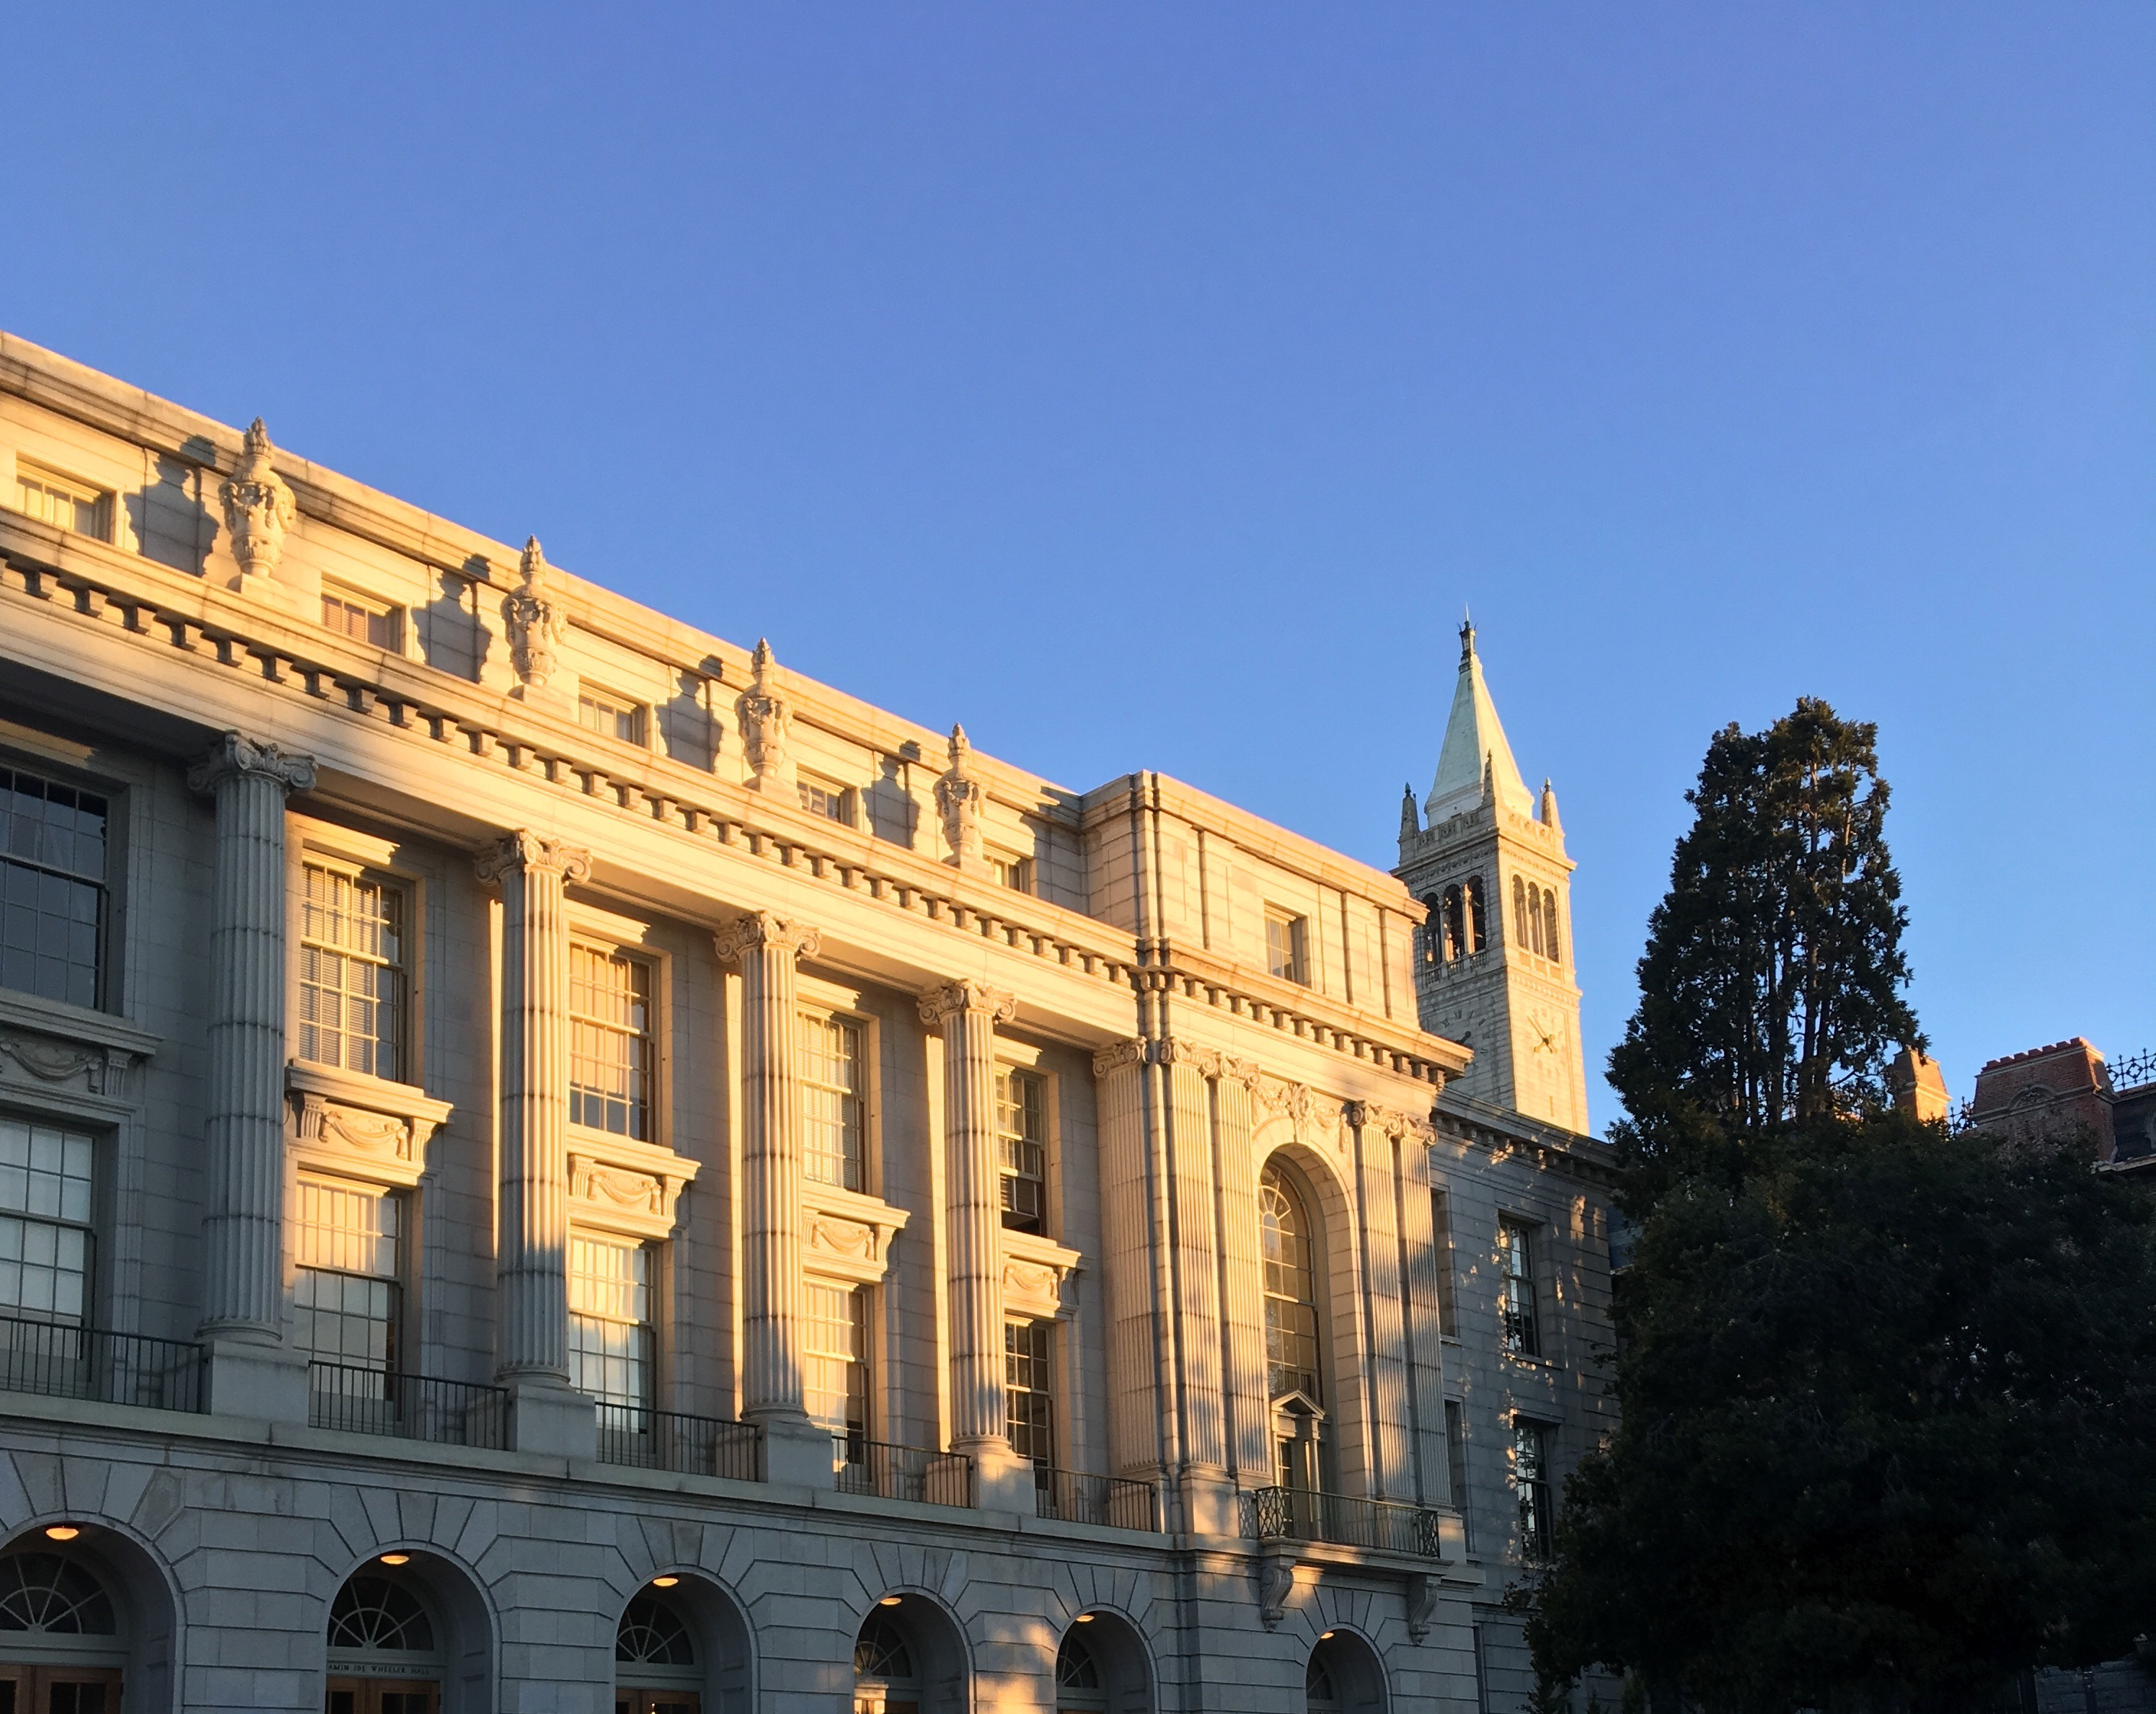
\includegraphics{./images/campus.jpeg}

This is the live session work space for the course. Our goal with this
repository, is that we're able to communicate \emph{ahead of time} our
aims for each week, and that you can prepare accordingly.

\part{Probabilty Theory}

Probability theory is the basis for all modeling in data science. In the
first part of the course, we will cover the basics.

\chapter{Probability Spaces}\label{probability-spaces}

\begin{Shaded}
\begin{Highlighting}[]
\FunctionTok{source}\NormalTok{(}\StringTok{\textquotesingle{}./src/blank\_lines.R\textquotesingle{}}\NormalTok{)}
\end{Highlighting}
\end{Shaded}

Probability is a system of reasoning about the world in the face of
incomplete information. In this course, we're going to develop an
understanding of the implications of core parts of this theory, how this
theory was developed, and how these implications relate to every other
part of the practice of data science.

\begin{figure}[H]

{\centering 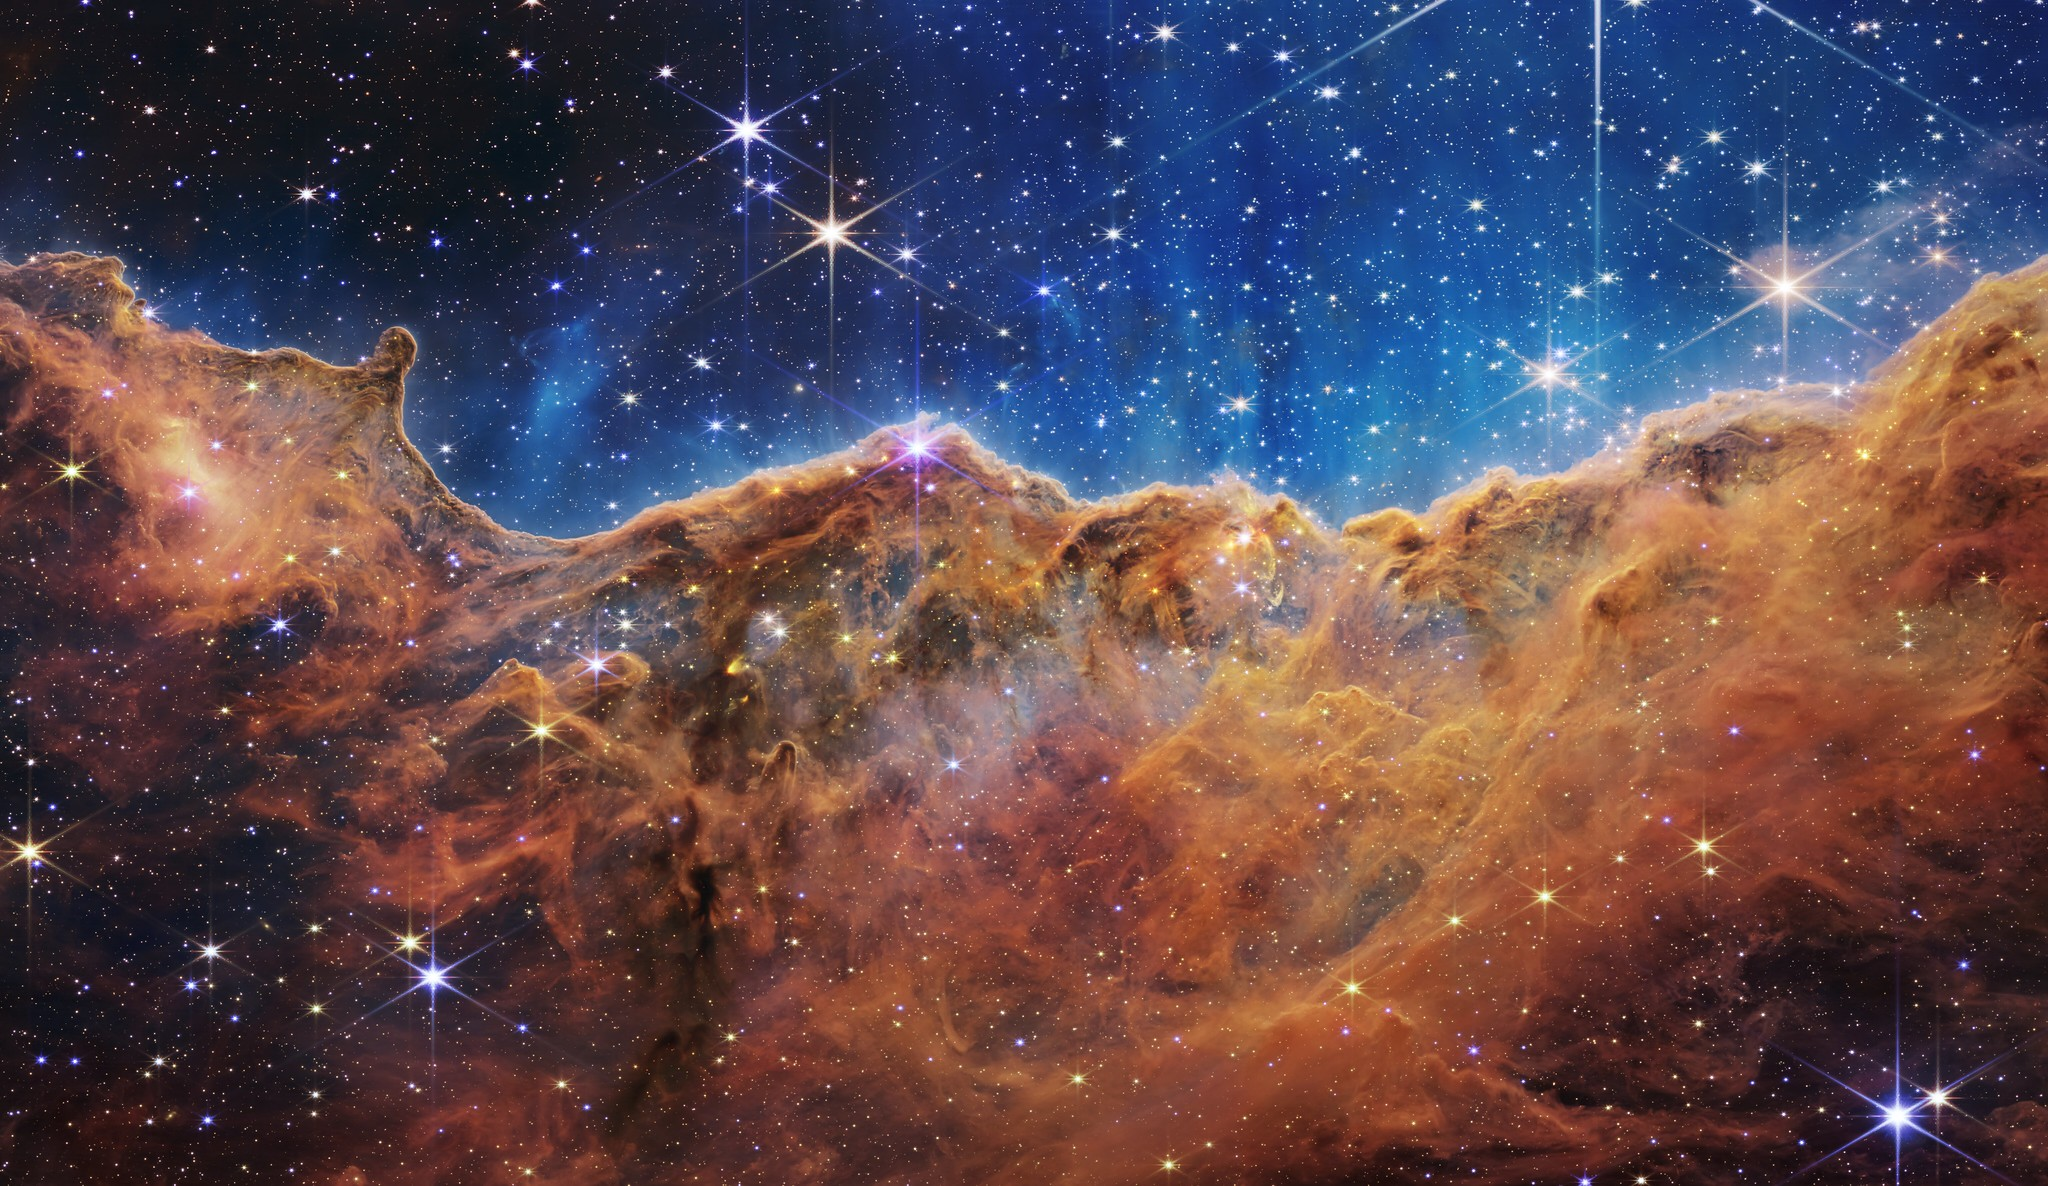
\includegraphics{./images/webb.jpg}

}

\caption{probability, the final frontier}

\end{figure}%

\section{Learning Objectives}\label{learning-objectives}

At the end of this week's learning, student will be able to:

\begin{enumerate}
\def\labelenumi{\arabic{enumi}.}
\tightlist
\item
  \textbf{Find} and \emph{access} all of the course materials;
\item
  \textbf{Develop} a course of study that is builds toward success;
\item
  \textbf{Apply} the axioms of probability to make a valid statement;
\item
  \textbf{Solve} word problems through the \emph{application} of
  probability and math rules.
\end{enumerate}

\section{Course Learning Objectives}\label{course-learning-objectives}

At this point in the course, there is so much that is before us! As we
settle in to study for the semester, it is useful to have a point of
view of where we're trying to go, and what we are going to see along the
way.

Allow a justification by analogy:

\begin{quote}
Suppose that you decide that you would like to be a chef -- all of the
time watching cooking shows has revealed to you that this is your life's
true calling -- and so you enroll in a culinary program.

One does not begin such a program by baking croissants and souffle. They
begin the program with knife skills, breaking down ingredients and the
basic techniques that build up to produce someone who is not a
\emph{cook}, but a \emph{chef} -- someone who can combine ingredients
and techniques to produce novel ideas.

At the same time, however, one has not gone to school just to become a
cucumber slicer. The knife skills are instrumental to the eventual goal
-- of being a chef -- but not the goal itself.
\end{quote}

At the beginning of the program, we're teaching these core, fundamental
skills. How to read and reason with mathematical objects, how to use
conditional probability with the goal of producing a model, and
eventually, \textbf{eventually} to create novel work as a data
scientist.

At the end of this course, students will be able to:

\subsection{Understand the building blocks of probability theory that
prepare learners for the study of statistical
models}\label{understand-the-building-blocks-of-probability-theory-that-prepare-learners-for-the-study-of-statistical-models}

\begin{enumerate}
\def\labelenumi{\arabic{enumi}.}
\tightlist
\item
  Understand the mathematical objects of probability theory and be able
  to apply their properties.
\item
  Understand how high-level concepts from calculus and linear algebra
  are related to common procedures in data science.
\item
  Translate between problems that are defined in business or research
  terms into problems that can be solved with math.
\end{enumerate}

\subsection{Understand and apply statistical models in common
situations}\label{understand-and-apply-statistical-models-in-common-situations}

\begin{enumerate}
\def\labelenumi{\arabic{enumi}.}
\tightlist
\item
  Understand the theory of statistics to prepare students for
  inferrential statements.
\item
  Understand model parameters and high level strategies to estimate
  them: means, least squares, and maximum likelihood.
\item
  Choose an appropriate statistic, and conduct a hypothesis test in the
  Neyman-Pearson framework.
\item
  Interpret the results of a statistical test, including statistical
  significance and practical significance.
\item
  Recognize limitations of the Neyman-Pearson hypothesis testing
  framework and be a conscientious participant in the scientific process
\end{enumerate}

\subsection{Analyze a research question using a linear regression
framework}\label{analyze-a-research-question-using-a-linear-regression-framework}

\begin{enumerate}
\def\labelenumi{\arabic{enumi}.}
\tightlist
\item
  Explore and wrangle data with the intention of understanding the
  information and relationships that are (and are not) present
\item
  Identify the goals of your analysis
\item
  Build a model that achieves the goals of an analysis
\end{enumerate}

\subsection{Interpret the results of a model and communicate them in
manner appropriate to the
audience}\label{interpret-the-results-of-a-model-and-communicate-them-in-manner-appropriate-to-the-audience}

\begin{enumerate}
\def\labelenumi{\arabic{enumi}.}
\tightlist
\item
  Identify their audience and report process and findings in a manner
  appropriate to that audience.
\item
  Construct regression oriented reports that provide insight for
  stakeholders.
\item
  Construct technical documents of process and code for collaboration
  and reproducability with peer data scientists.
\item
  Read, understand, and assess the claims that are made in technical,
  regression oriented reports
\end{enumerate}

\subsection{Contribute proficient, basic work, using industry standard
tools and coding practices to a modern data science
team.}\label{contribute-proficient-basic-work-using-industry-standard-tools-and-coding-practices-to-a-modern-data-science-team.}

Demonstrate programming proficiency by translating statistical problems
into code. 1. Understand and incorporate best practices for coding style
and data carpentry 2. Utilize industry standard tooling for
collaboration

\section{Introductions}\label{introductions}

\subsection{Instructor Introductions}\label{instructor-introductions}

The instructors for the course come to the program, and to statistics
from different backgrounds. Instructors hold PhDs in statistics,
astrophysics, biology, political science, computer science, and
information.

\subsection{What does a statistician look like?
You!}\label{what-does-a-statistician-look-like-you}

Identity shapes how people approach and understand their world.

We would like to acknowledge that we have limited diversity of identity
among the instructors for this course. We each have been fortunate to be
able to study, but we want to acknowledge that the education system in
the US has systematically benefited the hegemonic groups and
marginalized others voices.

Every one of the instructors shares a core identity as an empathetic
educator that wants to understand your strengths, areas for growth, and
unique point of view that is shaped by who you are. We want to see a
field of data scientists who embrace each others voices, and respects
people for the identies that they hold.

\begin{itemize}
\tightlist
\item
  It doesn't matter if you've never taken a stats class before, or if
  you're reviewing using this class. There will be challenges for
  everyone to overcome.
\item
  It doesn't matter how old or young you are. We will all be learning
  frequentist statistics which is timeless.
\item
  The color of your skin doesn't matter; nor does whether you identify
  as a woman or a man or trans or non-binary; neither does your sexual
  orientation. There are legacies of exclusion and discrimination
  against people due to these identities. We will not continue to
  propagate those legacies and instead will work to controvert those
  discriminations to build a diverse community of learning in line with
  the University's
  \href{https://diversity.berkeley.edu/principles-community}{Principles
  of Community}.
\end{itemize}

\section{Student Introductions {[}Breakout
One{]}}\label{student-introductions-breakout-one}

In a breakout room of between three and four students introduce
yourself!

\textbf{Breakout One.} A \emph{name story} is the unique, and individual
story that describes how you came to have the name that you do. While
there may be many people are called the same thing, each of their name
stories is unique.

Please share: \emph{What is your name story?}

\section{Student Introductions {[}Breakout
Two{]}}\label{student-introductions-breakout-two}

In the same breakout room:

\textbf{Breakout Two.} Like our names, the reasons that we joined this
program, our goals and our histories are different.

Please share: \emph{What is your data science story? How did you wind up
here, in this room today?}

\section{Probability Theory}\label{probability-theory}

\textbf{Probability}

Probability is a system of reasoning that we use to model the world
under incomplete information. This model underlies virtually
\emph{every} other model you'll ever use as a data scientist.

\begin{figure}[H]

{\centering 
\includegraphics{./images/picard.jpg}

}

\caption{told you this would be spacey}

\end{figure}%

In this course, probability theory builds out to random variables; when
combined with sampling theory we are able to develop p-values (which are
also random variables) and an inferential paradigm to communicate what
we know and how certain a statement we can make about it.

In introduction to machine learning, literally the first model that you
will train is a naive bayes classifier, which is an application of
Bayes' Theorem, trained using an iterative fitting algorithm. Later in
machine learning, you'll be fitting non-linear models, but at every
point the input data that you are supplying to your models are generated
from samples from random variables. That the world can be represented by
random variables (which we will cover in the coming weeks) means that
you can transform -- squeeze and smush, or stretch and pull -- variables
to heighten different aspects of the variables to produce the most
useful \emph{information} from your data.

As you move into NLP, you might think of generative text as a
conditional probability problem: given some particular set of words as
an input, what is the most likely \emph{next} word or words that someone
might type?

Beyond the direct instrumental value that we see working with
probability, there are two additional aims that we have in starting the
course in the manner.

First, because we are starting with the axioms of probability as they
apply to data science statistics, students in this course develop a
\emph{much} fuller understanding of classical statistics than students
in most other programs. Unfortunately, it is very common for students
and then professionals to see statistics as a series of rules that have
to be followed absolutely and without deviation. In this view of
statistics, there are distributions to memorize; there are repeated
problems to solve that require the rote application of some algebraic
rule (i.e.~compute the sample average and standard deviation of some
vector); and, there are myriad, byzantine statistical tests to memorize
and apply. In this view of statistics, if the real-world problem that
comes to you as a data scientist doesn't clearly fit into a box, there's
no way to move forward.

\begin{quote}
Statistics like this is not fun.
\end{quote}

In the way that we are approaching this course, we hope that you're able
to learn \emph{why} certain distributions (like the normal distribution)
arise repeatedly, and why we can use them. We also hope that because you
know how sampling theory and random variables combine, that you can be
more creative and inventive to solve problems that you haven't seen
before.

The second additional aim that we have for this course is that it can
serve as either an introduction or a re-introduction to reading and
making arguments using the language of math. For some, this will be a
new language; for others, it may have been some years since they have
worked with the language; for some, this will feel quite familiar. New
algorithms and data science model advancements \emph{nearly always}
developed in the math first, and then applied into algorithms second. In
our view, being a literate reader of graduate- and professional-level
math is a necessary skill for any data scientist that is going to keep
astride of the field as it continues to develop and these first weeks of
the course are designed to bring everyone back into reading and
reasoning in the language.

\section{Axiomatic Probability}\label{axiomatic-probability}

The book makes a point of defining our axioms of probability, calling
them them

\emph{Kolmogorov Axioms}

Let \(\Omega\) be a sample space, \(S\) be an event space, and \(P\) be
a probability measure. Then, \((\Omega, S, P)\) is a \emph{probability
space} if it satisfies the following:

\begin{itemize}
\tightlist
\item
  Non-negativity: \(\forall A \in S, P(A) \geq 0\), where \(P(A)\) is
  finite and real.
\item
  Unitarity: \(P(\Omega)=1\).
\item
  Countable additivity: if \(A_1, A_2, A_3, \dots \in S\) are pairwise
  disjoint, then
\end{itemize}

\[
P(A_1 \cup A_2 \cup A_3 \cup \dots) = P(A_1) + P(A_2) + P(A_3) = \sum_{i}P(A_{i})
\]

There is a lot going on in this definition!

First things first, these are the \textbf{axioms of probability} (read
aloud in the booming voice of a god).

This means that these are things that we begin from, sort of the
foundational principles of the entire system of reasoning that we are
going to use. In the style of argument that we're going to make, these
are things that are sort of off-limits to question. Instead, these serve
as the grounding assumptions, and we see what happens as we flow forward
from these statements.

Second, and importantly, from these axioms there are a \emph{very large}
set of things that we can build. The first set of things that we will
build are probability statements about atomic outcomes (Theorem 1.1.4 in
the book), and collections of events. But, these statements, are not the
only thing that we're limited to. We can also build \emph{Frequentist
Statistics}, and \emph{Bayesian Statistics} and \emph{Language Models}.

In many ways, these axioms are the fundamental particles that hold our
system of probabilistic reasoning together. These are to probability
what the \emph{fermions} and and \emph{bosons} are to physics.

\section{Definition vs.~Theorem}\label{definition-vs.-theorem}

What is the difference between a definition and a theorem? On pages 10
and 11 of the textbook, there is a rapid fire collection of pink boxes.
We reproduce them here (notice that they may have different index
numbers than the book -- this live session book autoindexes and we're
not including every theorem and definition in this live session
discussion guide).

\emph{Conditional Probability} For \(A, B \in S\) with \(P(B) > 0\), the
\emph{conditional probablity} of \(A\) given \(B\) is
\[P(A|B) = \frac{P(A\cap B)}{P(B)}.\]

\emph{Multiplicative Law of Probability} For \(A, B \in S\) with
\(P(B) > 0\), \[P(A|B)P(B) = P(A \cap B)\]

\emph{Baye's Rule} For \(A, B \in S\) with \(P(A) > 0\) and
\(P(B) > 0\), \[P(A|B) = \frac{P(B|A)P(A)}{P(B)}.\]

\begin{itemize}
\tightlist
\item
  What would happen to the statement of the \emph{Multiplicative Law of
  Probability} if we did not have the definition of \emph{Conditional
  Probability}?
\item
  How does one get from the definition, to the law?
\item
  Can one get to \emph{Baye's Rule} wihtout using the
  \emph{Multiplicative Law of Probability}?
\end{itemize}

\section{Working with a Sample Space}\label{working-with-a-sample-space}

As a way to begin lets define terms that we will use for the next
activities.

\textbf{Group Discussion Question}

\begin{itemize}
\tightlist
\item
  What is the definition of a sample space?
\item
  What is the definition of an event?
\item
  How are sample spaces, and event spaces related?
\end{itemize}

\subsection{Working with a Sample Space, Part
I}\label{working-with-a-sample-space-part-i}

\begin{enumerate}
\def\labelenumi{\arabic{enumi}.}
\tightlist
\item
  \textbf{You roll two six-sided dice}:

  \begin{enumerate}
  \def\labelenumii{\arabic{enumii}.}
  \tightlist
  \item
    How would you define an appropriate sample space, \(\Omega\)?
  \item
    How many elements exist in \(\Omega\)?
  \item
    What is an appropriate event space, and how many elements does it
    have?
  \item
    Give an example of an event.
  \end{enumerate}
\end{enumerate}

\vspace{5cm}

\subsection{Working with a Sample Space, Part
II}\label{working-with-a-sample-space-part-ii}

\begin{enumerate}
\def\labelenumi{\arabic{enumi}.}
\setcounter{enumi}{1}
\tightlist
\item
  \textbf{For a random sample of 1,000 Berkeley students}:

  \begin{enumerate}
  \def\labelenumii{\arabic{enumii}.}
  \tightlist
  \item
    How would you define an appropriate sample space, \(\Omega\)?
  \item
    How big is \(\Omega\)? How many elements does it contain?
  \item
    What is an example of an event for this scenario?
  \item
    Can a single person be represented in the space twice? Why or why
    not?
  \end{enumerate}
\end{enumerate}

\vspace{5cm}

\section{Independence}\label{independence}

The book provides a (characteristically) terse statement of what it
means for two events to be independent of one another.

\emph{Independence of Events} Events \(A, B \in S\) are
\emph{independent} if \[P(A \cap B) = P(A)P(B)\].

In your own words:

\begin{itemize}
\tightlist
\item
  What does it mean for two events to be independent of one another?
\item
  How do you \textbf{know} if two events are independent of one another?
\item
  How do you \textbf{test} if two events are independent of one another?
\end{itemize}

Try using this idea of independent in two places:

\begin{enumerate}
\def\labelenumi{\arabic{enumi}.}
\tightlist
\item
  Suppose that you are creating a model to predict an outcome. Further,
  suppose that two events \(A\) and \(B\) are independent of one
  another. \emph{Can you use \(B\) to predict \(A\)}?
\item
  If two events, \(A\) and \(B\) are independent, then what happens if
  you work through a statement of conditional probability, \(P(A|B)\)?
\end{enumerate}

\section{A practice problem}\label{a-practice-problem}

The last task for us to complete today is working through a practice
problem on the course practice problem website. Please, click the link
below, and follow us over to the the course's practice problem website.

\href{https://mids-w203.github.io/practice_problems/}{link here}

\section{Student Tasks to Complete}\label{student-tasks-to-complete}

Before next live session, please complete the homework that builds on
this unit. There are two parts, an \emph{applied} and a \emph{proof}
part. You can submit these homework as many times as you like before the
due date (you will not receive feedback), and you can access this
homework through bCourses.

The \emph{applied} homework will be marked either \texttt{Correct} or
\texttt{Incorrect} without partial credit applied. These are meant to be
problems that you solve, and that have a single straightforward solution
concept. The \emph{proof} homework will be marked for partial credit
(out of three points) that evaluates your argument for your solution
concept.

\chapter{Defining Random Variables}\label{defining-random-variables}

\begin{verbatim}
-- Attaching core tidyverse packages ------------------------ tidyverse 2.0.0 --
v dplyr     1.1.3     v readr     2.1.4
v forcats   1.0.0     v stringr   1.5.0
v ggplot2   3.4.4     v tibble    3.2.1
v lubridate 1.9.3     v tidyr     1.3.0
v purrr     1.0.2     
-- Conflicts ------------------------------------------ tidyverse_conflicts() --
x purrr::%||%()   masks base::%||%()
x dplyr::filter() masks stats::filter()
x dplyr::lag()    masks stats::lag()
i Use the conflicted package (<http://conflicted.r-lib.org/>) to force all conflicts to become errors

Attaching package: 'plotly'


The following object is masked from 'package:ggplot2':

    last_plot


The following object is masked from 'package:stats':

    filter


The following object is masked from 'package:graphics':

    layout
\end{verbatim}

\begin{figure}[H]

{\centering \includegraphics{./images/yosemite.jpg}

}

\caption{yosemite valley}

\end{figure}%

\section{Learning Objectives}\label{learning-objectives-1}

At the end of this week's course of study (which includes the async,
sync, and homework) students should be able to

\begin{enumerate}
\def\labelenumi{\arabic{enumi}.}
\tightlist
\item
  \textbf{Remember} that random variable are neither random, or
  variables, but instead that they are objects thare are a foundation
  that we can use to reason about a world.
\item
  \textbf{Understand} that the intuition developed by the use of
  set-theory probability maps into the more expressive space of random
  variables
\item
  \textbf{Apply} the appropriate mathematical transformations to move
  between joint, marginal, and conditional distributions.
\end{enumerate}

This week's materials are theoretical tooling to build toward one of the
first notable results of the course, \textbf{conditional probability}.
This is the idea that, if we know that one event has occurred, we can
make a conditional statement about the probability distribution for
another, dependent distribution.

\section{Introduction to the
Materirals}\label{introduction-to-the-materirals}

From the axioms of probability, it is possible to build a whole,
expressive modeling system (that need not be grounded \textbf{at all} in
the minutia of the world). With this probability model in place, we can
describe how frequently events in the random variable will occur. When
variable are dependent upon each other, we can utilize information that
is encoded in this dependence in order to make predictions that are
\emph{closer to the truth} than predictions made without this
information.

There is both a beauty and a tragedy when reasoning about random
variables: we describe random variables using their joint density
function.

\begin{itemize}
\tightlist
\item
  The \textbf{beauty} is that by reasoning with such general objects --
  the definitions that we create, and the theorems that we derive in
  this section of the course -- produce guarantees that hold in every
  case, no matter the function that stands in for the joint density
  function. We will compute several examples of \emph{specific}
  functions to provide a chance to reason about these objects and how
  they ``work''.
\item
  The \textbf{tragedy} is that in the ``real world'', the world where we
  are going to eventually going to train and deploy our models, we are
  never provided with this joint density function. Because we don't have
  access to the joint density function, in later weeks we will try to
  produce estimates using data. The simpler the estimate, the less data
  we need; the fuller the representation of the joint density function
  we desire, the more data we need.
\end{itemize}

Perhaps this is the creation myth for probability theory: in a perfect
world, we can produce a perfect result. But, in the ``fallen'' world of
data, we will only be able to produce approximations.

\section{Class Announcements}\label{class-announcements}

\subsection*{Homework}\label{homework}
\addcontentsline{toc}{subsection}{Homework}

\begin{enumerate}
\def\labelenumi{\arabic{enumi}.}
\tightlist
\item
  You should have turned in your first homework. The solution set for
  this homework is scheduled to be released to you in Thursday at 2:00p.
  The solution set contains a full explanation of how we solved the
  questions posed to you. You can expect that feedback for this homework
  will be released back to you within seven days.
\item
  You can start working on your second homework when we are out of this
  class.
\end{enumerate}

\subsection*{Study Groups}\label{study-groups}
\addcontentsline{toc}{subsection}{Study Groups}

It is a \textbf{very} good idea for you to create a recurring time to
work with a set of your classmates. Working together will help you solve
questions more effectively, quickly, and will also help you to learn how
to communicate what you do and do not understand about a problem to a
group of collaborating data scientists. And, working together with a
group will help you to find people who share data science interests with
you.

\subsection*{Course Resources}\label{course-resources}
\addcontentsline{toc}{subsection}{Course Resources}

There are several resources to support your learning. A learning object
last week was that you would be introduced to each of these systems.
Please continue to make sure that you have access to the:

\begin{itemize}
\tightlist
\item
  \href{https://www.lib.berkeley.edu/using-the-libraries/vpn}{Library
  VPN} to read all of the scholarly content in the known universe,
  including the course textbook.
\item
  \href{https://www.bcourses.berkeley.edu}{Course LMS Page}
\end{itemize}

\section{Using Definitions of Random
Variables}\label{using-definitions-of-random-variables}

\subsection{Random Varaible}\label{random-varaible}

What is a random variable? Does this definition help you?

A random variable is a function \(X : \Omega \rightarrow \mathbb{R},\)
such that
\(\forall r \in \mathbb{R}, \{\omega \in \Omega: X(\omega) \leq r\} \in S\).

Someone, please, read that without using a single ``omega'',
\(\mathbb{R}\), or other jargon terminology. Instead, someone read this
aloud and tell us what each of the concepts mean.

\begin{tcolorbox}[enhanced jigsaw, titlerule=0mm, opacitybacktitle=0.6, colframe=quarto-callout-note-color-frame, bottomrule=.15mm, leftrule=.75mm, breakable, bottomtitle=1mm, coltitle=black, toptitle=1mm, colback=white, opacityback=0, arc=.35mm, left=2mm, rightrule=.15mm, toprule=.15mm, title=\textcolor{quarto-callout-note-color}{\faInfo}\hspace{0.5em}{Note}, colbacktitle=quarto-callout-note-color!10!white]

You might notice that the \(X(\omega) \leq r\) feels kind of weird; why
isn't it just \(X(\omega) = r\)? After all, this is a mapping from an
outcome, \(\omega \in \Omega\) to a real number, right? So, why not just
be direct about it? The answer is a real deep-dive, and one that is
better suited to a formal measure theory course.

The short answer, is that the we use this \(\leq r\) range because we're
using a \href{https://en.wikipedia.org/wiki/Borel_set}{Boreal \(\sigma\)
algebra} to constrain the sets that have probability measures. Why this
constraint? If we don't weird stuff can happen. Like, real weird things:
you can split a sphere into pieces and create two new spheres of equal
volume from the pieces
(\href{https://en.wikipedia.org/wiki/Banach–Tarski_paradox}{Banch-Tarski
Paradox}).

\end{tcolorbox}

The goal of writing with math symbols like this is to be
\emph{absolutely} clear what concepts the author does and does not mean
to invoke when they write a definition or a theorem. In a very real
sense, this is a language that has specific meaning attached to specific
symbols; there is a correspondence between the mathematical language and
each of our home languages, but exactly what the relationship is needs
to be defined into each student's home language.

\begin{itemize}
\tightlist
\item
  What are the key things that random variables allow you to accomplish?

  \begin{itemize}
  \tightlist
  \item
    Suppose that you were going to try to make a model that predicts the
    probability of winning ``big money'' on a slot machine. Big money
    might be that you get 🍒🍒🍒. Can you do \emph{math} with 🍒?
  \item
    Suppose that you wanted to build a chatbort that uses a language
    model so that you don't have to do your homework anymore. How would
    you go about it? Can you do math on words or concepts?
  \item
    Suppose you want to direct class support to students in 203, but
    their grades are scored \texttt{{[}A,\ A-,\ ...,\ C+{]}} and
    features include prior statistics classes grades, also scored
    \texttt{A,\ A-,\ ...,\ C+{]}.}
  \end{itemize}
\end{itemize}

\section{Pieces of a Random Variable}\label{pieces-of-a-random-variable}

A random variable is a function \(X : \Omega \rightarrow \mathbb{R},\)
such that
\(\forall r \in \mathbb{R}, \{\omega \in \Omega\}: X(\omega) \leq r\} \in S\).

There are two key pieces that must exist for every random variable. What
are these pieces? The new piece is provided to us in \textbf{Definition
1.2.1} \emph{Random Variable} (on page 16). The older piece (from last
week) that is now useful is a part of the Kolmogorov Axiom, the
probabilty triple: \((\Omega, S, P)\) where \(\Omega\) is a sample
space, \(S\) is an event space, and \(P\) is a probability-measure.

\begin{enumerate}
\def\labelenumi{\arabic{enumi}.}
\tightlist
\item
\item
\end{enumerate}

Suppose that a random variable is simple and discrete. For concreteness,
you could think of this random variable as the answer to the question,
``Is the grass wet outside?''.

\begin{enumerate}
\def\labelenumi{\arabic{enumi}.}
\tightlist
\item
  What is the sample space?
\item
  What is a sensible function that you might use to map from the sample
  space to real values?
\item
  What is a sensible function that you might use to map from the sample
  space to real values? (A student well-seasoned in Maths might use (and
  define for the rest of the class) the concept of a \emph{bijective
  function}).
\item
  If you simply had the values that the random variable function maps to
  are you guaranteed to be able to describe the entire sample space? Why
  or why not?
\item
  How would you go about determining the probability mass function for
  this random variable?
\end{enumerate}

\subsection{Functions of Functions}\label{functions-of-functions}

Why do we say that random variables are functions? Is there some useful
property of these being functions rather than any other quantity? What
else \emph{could} they be if not a function?

What about a function of a random variable, which is a function of a
function.

Let \(g : U \rightarrow \mathbb{R}\) be some function, where
\(X(\Omega) \subseteq U \subseteq \mathbb{R}\). Then, if
\(g \circ X : \Omega \rightarrow \mathbb{R}\) is a random variable, we
say that \(g\) is a \emph{function} of X and write \(g(X)\) to denote
the random variable \(g \circ X\).

If a random variable is a function from the real world, or the sample
space, or the outcome space to a real number, then what does it mean to
define a function of a random variable?

\begin{itemize}
\tightlist
\item
  At what point does this function work? Does this function change the
  sample space that is possible to observe? Or, does this function
  change the real-number that each outcome points to?
\end{itemize}

Suppose that you are doing some image processing work. To keep things
simple, that you are doing image classification in the style of the
MNIST dataset.

\begin{itemize}
\tightlist
\item
  Can someone describe what this task is trying to accomplish?
\item
  Has anyone done work like this?
\end{itemize}

However, suppose that rather than having good clean indicators for
whether a pixel is on or off, instead you have weak indicators --
there's a lot of grey. A lot of the cells are marked in the range
\(0.2 - 0.3\).

\begin{enumerate}
\def\labelenumi{\arabic{enumi}.}
\tightlist
\item
  How might creating a function that re-maps this grey into more extreme
  values help your model?
\item
  Is it possible to ``blur'' events that are in the outcome space? Does
  this ``blurring'' meet the requirements of a function of a random
  variable, as provided above?
\end{enumerate}

\subsection{Probability Density Functions and Cumulative Distribution
Functions}\label{probability-density-functions-and-cumulative-distribution-functions}

\begin{itemize}
\tightlist
\item
  What is a probability mass function?
\item
  What do the \textbf{Kolmogorov Axioms} mean must be true about any
  probability mass function (\emph{pmf})?
\end{itemize}

You should try driving in Berkeley some time. It is a \textbf{trip}!
Without being deliberately ageist, the city is full of ageing hippies
driving beater Subaru Outbacks and making what seem to be stochastic
right-or-left turns to buy incense, pottery, or just sourdough bread.

Suppose that you are walking to campus, and you have to cross 10
crosswalks, each of which are spaced a block apart. Further, suppose
that as you get closer to campus, there are fewer aging hippies, and
therefore, there is decreasing risk that you're hit by a Subaru as you
cross the street. Specifically, and fortunately for our math, the risk
of being hit decreases linearly with each block that you cross.

Finally, campus provides you with the safety reports from last year, and
reports that there were 55 student-Subaru incidents last year, out of
10,000 student-crosswalk crossings.

\begin{enumerate}
\def\labelenumi{\arabic{enumi}.}
\tightlist
\item
  What is the \emph{pmf} for the probability that you are involved in a
  student-Subaru incident as you walk across these 10 blocks? What
  sample space, \(\Omega\) is appropriate to represent this scenario?
\item
  Suppose that you don't leave your house -- this is a remote program
  after all! What is your cumulative probability of being involved in a
  student-subaru incident?
\item
  What is the cumulative probability \emph{cmf} for the probability that
  you are involved in a student-Subaru incident?
\item
  Suppose that you live three blocks from campus, but your classmate
  lives five blocks from campus. What is the difference in the
  cumulative probability?
\item
  How would you describe the cumulative probability of being hit as you
  walk closer to campus? That is, suppose that you start 10 blocks away
  from campus, and are walking to get closer. Is your cumulative
  probability of being hit on your way to campus increasing or
  decreasing as you get closer to campus?
\item
  How would you describe the cumulative probability of being hit as you
  walk \textbf{further} from campus? That is, suppose that you start on
  campus, and you're walking to a bar after classes. Is your cumulative
  probability of being hit on your way away from campus increasing or
  decreasing as you get further from campus?
\end{enumerate}

\section{Discrete \& Continuous Random
Variables}\label{discrete-continuous-random-variables}

What, if anything is fundamentally different between discrete and
continuous random variables? As a way of starting the conversation,
consider the following cases:

\begin{itemize}
\tightlist
\item
  Suppose \(X\) is a random variable that describes the time a student
  spends on w203 homework 1.

  \begin{itemize}
  \tightlist
  \item
    If you have only granular measurement -- i.e.~the number of nights
    spent working on the homework -- is this discrete or continuous?
  \item
    If you have the number of hours, is it discrete or continuous?
  \item
    If you have the number of seconds? Or milliseconds?
  \end{itemize}
\item
  Is it possible that \(P(X = a) = 0\) for every point \(a\)? For
  example, that \(P(X = 3600) = 0\).
\item
  Does one of these measures have more \emph{information} in it than
  another?

  \begin{itemize}
  \tightlist
  \item
    How are measurement choices that we make as designers of information
    capture systems -- i.e.~the machine processes, human processes, or
    other processes that we are going to work with as data scientists --
    reflected in both the amount of information that is gathered, the
    type of information that is gathered, and the types of random
    variables that are manifest as a result?
  \end{itemize}
\end{itemize}

\section{Moving Between PDF and CDF}\label{moving-between-pdf-and-cdf}

The book defines \emph{pmf} and \emph{cmf} first as a way of developing
intuition and a way of reasoning about these concepts. It then moves to
defining continuous density functions, which is many ways are easier to
work with although they lack the means of reasoning about them
intuitively. Continuous distributions are defined in the book, and more
generally, in terms of the \emph{cdf}, which is the cumulative
distribution function. There are technical reasons for this choice of
definition, some of which are signed in the footnotes on the page where
the book presents it.

More importantly for this course, in \textbf{Definition 1.2.15} the book
defines the relationship between \emph{cdf} and \emph{pdf} in the
following way:

For a continuous random variable \(X\) with CDF \(F\), the
\emph{probability density function} of \(X\) is

\[
  f(x) = \left. \frac{d F(u)}{du} \right|_{u=x}, \forall x \in \mathbb{R}.
\]

The implies, further, that for a random variable \(X\) with PDF \(f\),
the \emph{cumulative density function} of \(X\) is:

\[
F(x) = \int f(x) dx, \forall x \in \mathbb{R}. 
\]

\begin{itemize}
\tightlist
\item
  How does this definition, which relates \emph{pdf} and \emph{cdf} by a
  means of differentiation and integration, fit with the ideas that we
  just developed in the context of walking to and from campus?
\end{itemize}

Suppose that you learn than a particular random variable, \(X\) has the
following function that describes its \emph{pdf},
\(f_{x}(x) = \frac{1}{10}x\). Also, suppose that you know that the
smallest value that is possible for this random variable to obtain is 0.

\begin{enumerate}
\def\labelenumi{\arabic{enumi}.}
\tightlist
\item
  What is the CDF of \(X\)?
\item
  What is the maximum possible value that \(x\) can obtain? How did you
  develop this answer, using the Kolmogorov axioms of probability?
\item
  What is the cumulative probability of an outcome up to 0.5?
\item
  What is the probability of an outcome between 0.25 and 0.75? Produce
  an answer to this in two ways:

  \begin{enumerate}
  \def\labelenumii{\arabic{enumii}.}
  \tightlist
  \item
    Using the \(PDF\)
  \item
    Using the \(CDF\)
  \end{enumerate}
\end{enumerate}

\section{Joint Density}\label{joint-density}

Working with a single random variable helps to develop our understanding
of how to relate the different features of a \emph{pdf} and a \emph{cdf}
through differentiation and integration. However, there's not really
\emph{that} much else that we can do; and, there is probably very little
in our professional worlds that would look like a single random variable
in isolation.

We really start to get to something useful when we consider joint
density functions. Joint density functions describe the probability that
\emph{both} of two random variables. That is, if we are working with
random variables \(X\) and \(Y\), then the joint density function
provides a probability statement for \(P(X \cap Y)\).

In this course, we might typically write this joint density function as
\(f_{X,Y}(x,y) = f(\cdot)\) where \(f(\cdot)\) is the actual function
that represents the joint probability. The \(f(\cdot)\) means,
essentially, ``some function'' where we just have not designated the
specifics of the function; you might think of this as a generic
function.

\subsection{Example: Uniform Joint
Density}\label{example-uniform-joint-density}

Suppose that we know that two variables, \(X\) and \(Y\) are jointly
uniformly distributed within the the \emph{support}
\(x \in [0,4], y \in [0,4]\). We have a requirement, imposed by the
\emph{Kolmogorov Axioms} that all probabilities must be non-zero, and
that the total probability across the whole support must be one.

\begin{itemize}
\tightlist
\item
  Can you use these facts to determine answers to the following:

  \begin{itemize}
  \tightlist
  \item
    What kind of shape does this joint \emph{pdf} have?
  \item
    What is the specific function that describes this shape?
  \item
    If you draw this shape on three axes, and \(X\), and \(Y\), and a
    \(P(X,Y)\), what does this plot look like?
  \item
    How do you get from the joint density function, to a marginal
    density function for \(X\)?
  \item
    How do you get form the joint density function, to a marginal
    density function for \(Y\)?
  \item
    How do you get from these marginal density functions of \(X\) and
    \(Y\) back to the joint density? Is this always possible?
  \end{itemize}
\end{itemize}

\subsection{Examples: Thinking Through Many
Plots}\label{examples-thinking-through-many-plots}

\includegraphics{02-random-variables_files/figure-pdf/unnamed-chunk-1-1.pdf}

\subsection{Triangle Math}\label{triangle-math}

After considering the intuition for the triangle distribution, do the
following: Write down the function that accords with the figure that
you're seeing above.\footnote{Notice, that in general, this kind of
  \emph{curve fitting} isn't really a common data science task. Instead,
  this is just a learning task that lets the class assess their
  understanding of the definitions of random variables.}

\begin{itemize}
\tightlist
\item
  What is a full statement of the PDF of this image?
\item
  What is the marginal distribution of \(X\), \(f_{X}(x)\)?
\item
  What is the marginal distribution of \(Y\), \(f_{Y}(y)\)?
\item
  Using the definition of independence, are \(X\) and \(Y\) independent
  of each other?
\item
  What is the CDF of \(X\), \(F_{X}(x)\)?
\end{itemize}

\subsection{Saddle Sores}\label{saddle-sores}

Suppose that you know that two random variables, \(X\) and \(Y\) are
jointly distributed with the following \emph{pdf}:

\[
f_{X,Y}(x,y) =
  \begin{cases}
    a * x^{2} * y^{2}, & 0 < x < 1, 0 < y < 1 \\
    0, & \text{otherwise.}
  \end{cases}
\]

This joint pdf is similar to the pdf that you can visualize above, under
the distribution called ``saddle''. The difference between this function
and the image above is that the function bounds the with support of
\(x\) and \(y\) on the range \([0,1]\). This is to make the math easier
for us in the next step.

\begin{itemize}
\tightlist
\item
  Can you use these facts to determine the following?

  \begin{itemize}
  \tightlist
  \item
    What value of \(a\) makes this a valid joint pdf?
  \item
    What is the marginal pdf of \(x\)? That is, what is \(f_{x}(x)\)?
  \item
    What is the conditional pdf of \(X\) given \(Y\)? That is, what is
    \(f_{x|y}(x,y)\)?
  \item
    Given these facts, would you say that \(X\) and \(Y\) are dependent
    or independent?
  \item
    If the support for this joint distribution were instead \([0,4]\)
    (rather than \([0,1]\)), how would the shape of the distribution
    change?
  \end{itemize}
\end{itemize}

\section{Computing Different
Distributions.}\label{computing-different-distributions.}

Suppose that random variables \(X\) and \(Y\) are jointly continuous,
with joint density function given by,

\[
f(x,y) = 
  \begin{cases}
    c, & 0 \leq x \leq 1, 0 \leq y \leq x \\
    0, & otherwise
\end{cases}
\]

where \(c\) is a constant.

\begin{enumerate}
\def\labelenumi{\arabic{enumi}.}
\tightlist
\item
  Draw a graph showing the region of the X-Y plane with positive
  probability density.
\item
  What is the constant \(c\)?
\item
  Compute the marginal density function for \(X\). (Be sure to write a
  complete expression)
\item
  Compute the conditional density function for \(Y\), conditional on
  \(X=x\). (Be sure to specify for what values of \(x\) this is defined)
\end{enumerate}

\section{Conditional Probability}\label{conditional-probability}

Conditional probability is \textbf{incredible}. In fact, without
exaggeration, almost \textbf{all} of data science is an exercise in
making statements about conditional probability distributions.
\emph{Don't believe us?}

\begin{itemize}
\tightlist
\item
  What is the goal of a ``customer churn'' model or a conversion model?
\item
  What is the goal of a language-completion model?
\item
  What is the goal of flight-departures model?
\end{itemize}

\textbf{If} we possessed the whole information about a process;
\textbf{if} we had the CDF that governed probability of occurrences,
what kinds of statements would we be able to make? Would we even need
data?

Using the distribution above, produce a statement of conditional
probability, \(f_{Y|X}(y|x)\).

\section{Visualizing Distributions Via
Simulation}\label{visualizing-distributions-via-simulation}

To this point in the course, we have focused on concepts in ``the
population'' with no reference to samples. This is on purpose! We want
to develop the theory that defines the \textbf{best possible} predictor
if we knew \textbf{everything} (if we know formula of the function that
maps from \(\omega \rightarrow \mathbb{R}\), and we know the probability
of each \(\omega \in \Omega\) then we know everything). Beginning in
week 5 of the course, we will talk about ``approximating'' (which we
will call estimating) this best possible predictor with a limited sample
of data.

However, at this point, to help build your working understanding, or
intuition, for what is happening, we are going to work on a way to
\emph{simulate} draws from a population. In some places, people might
refer to these as \emph{Monte Carlo} methods -- this is because the
method was developed by von Neumann \& Ulam during World War II, and
they needed a way to talk about it using a code name. They chose
\emph{Monte Carlo} after a famous casino in Monaco.

\subsection{Example: The Uniform
Distribution}\label{example-the-uniform-distribution}

\begin{quote}
You: ``Gosh. There sure are a lot of examples that use the uniform
distribution. That must be a really important statistical
distribution.''

Instructor: ``Nah. Not really. We're just using the uniform a bunch so
that we don't get too lost in doing math while we're working with these
concepts.''
\end{quote}

We'll start with a simple uniform distribution, but then we'll make it a
little more complex in a moment.

We can use R to simulate draws from a probability distribution function
by providing it with the name of the distribution that we're
considering, the support of that distribution, or other features of the
distribution. In the case of the uniform, the entire distribution is can
be described just from it support.

So, suppose that you had a uniform distribution that had positive
probability on the range \([1.1, 4.3]\). Why these? No particular
reason. That is, suppose

\[
f_{X}(x) =
  \begin{cases} 
    a & 1.1 \leq x \leq 4.3 \\ 
    0 & otherwise
  \end{cases}
\]

What does this distribution ``look like''? Because it is a uniform, you
might have a sense that it will be a horizontal line. But, what is the
height of that line? Aha! We could do the math to figure it out, or we
could generate an approximation using a simulation.

In the code below, we are going to create an object called
\texttt{samples\_uniform} that stores the results of the \texttt{runif}
function call.

\begin{Shaded}
\begin{Highlighting}[]
\NormalTok{samples\_uniform }\OtherTok{\textless{}{-}} \FunctionTok{runif}\NormalTok{(}\AttributeTok{n=}\DecValTok{1000}\NormalTok{, }\AttributeTok{min=}\FloatTok{1.1}\NormalTok{, }\AttributeTok{max=}\FloatTok{4.3}\NormalTok{)}
\end{Highlighting}
\end{Shaded}

What is happening inside \texttt{runif}?

When you're writing you own code, you can pull up the documentation for
this (and any) function using a question mark, i.e.~\texttt{?}, followed
by the function name -- \texttt{?runif}.

But, we can speed this up slightly by simply telling you that \texttt{n}
is the number of samples to take from the population; \texttt{min} is
the low-end of the support, and \texttt{max} is the high-end of the
support.

If we look into this object, we can see the results of the function
call. Below, we will show the first \(20\) elements of the
\texttt{samples\_uniform} object.

\begin{Shaded}
\begin{Highlighting}[]
\NormalTok{samples\_uniform[}\DecValTok{1}\SpecialCharTok{:}\DecValTok{20}\NormalTok{]}
\end{Highlighting}
\end{Shaded}

\begin{verbatim}
 [1] 1.614028 1.455171 2.095655 2.082238 2.506946 2.957886 3.452067 1.765094
 [9] 4.164895 1.448327 1.769607 1.659020 2.894359 3.193325 2.511176 2.090183
[17] 1.112637 2.649366 3.657755 3.560751
\end{verbatim}

(Notice that R is a \(1\) index language (python is a zero-index
language).)

With this object created, we can plot a density of the data and then
learn from this histogram what the pdf looks like.

\begin{Shaded}
\begin{Highlighting}[]
\NormalTok{plot\_full\_data }\OtherTok{\textless{}{-}} \FunctionTok{ggplot}\NormalTok{() }\SpecialCharTok{+} 
  \FunctionTok{aes}\NormalTok{(}\AttributeTok{x=}\DecValTok{1}\SpecialCharTok{:}\FunctionTok{length}\NormalTok{(samples\_uniform), }\AttributeTok{y=}\NormalTok{samples\_uniform) }\SpecialCharTok{+} 
  \FunctionTok{geom\_point}\NormalTok{()  }\SpecialCharTok{+} 
  \FunctionTok{labs}\NormalTok{(}
    \AttributeTok{title =} \StringTok{\textquotesingle{}Showing the Data\textquotesingle{}}\NormalTok{, }
    \AttributeTok{y     =} \StringTok{\textquotesingle{}Sample Value\textquotesingle{}}\NormalTok{, }
    \AttributeTok{x     =} \StringTok{\textquotesingle{}Index\textquotesingle{}}\NormalTok{)}

\NormalTok{plot\_density }\OtherTok{\textless{}{-}} \FunctionTok{ggplot}\NormalTok{() }\SpecialCharTok{+} 
  \FunctionTok{aes}\NormalTok{(}\AttributeTok{x=}\NormalTok{samples\_uniform) }\SpecialCharTok{+} 
  \FunctionTok{geom\_density}\NormalTok{(}\AttributeTok{bw=}\FloatTok{0.1}\NormalTok{)   }\SpecialCharTok{+} 
  \FunctionTok{labs}\NormalTok{(}
    \AttributeTok{title =} \StringTok{\textquotesingle{}Showing the PDF\textquotesingle{}}\NormalTok{, }
    \AttributeTok{y     =} \StringTok{\textquotesingle{}Probability of Drawing Value\textquotesingle{}}\NormalTok{, }
    \AttributeTok{x     =} \StringTok{\textquotesingle{}Sample Value\textquotesingle{}}\NormalTok{)}

\NormalTok{(plot\_full\_data }\SpecialCharTok{|}\NormalTok{ (plot\_density }\SpecialCharTok{+} \FunctionTok{coord\_flip}\NormalTok{())) }\SpecialCharTok{/} 
\NormalTok{  plot\_density }
\end{Highlighting}
\end{Shaded}

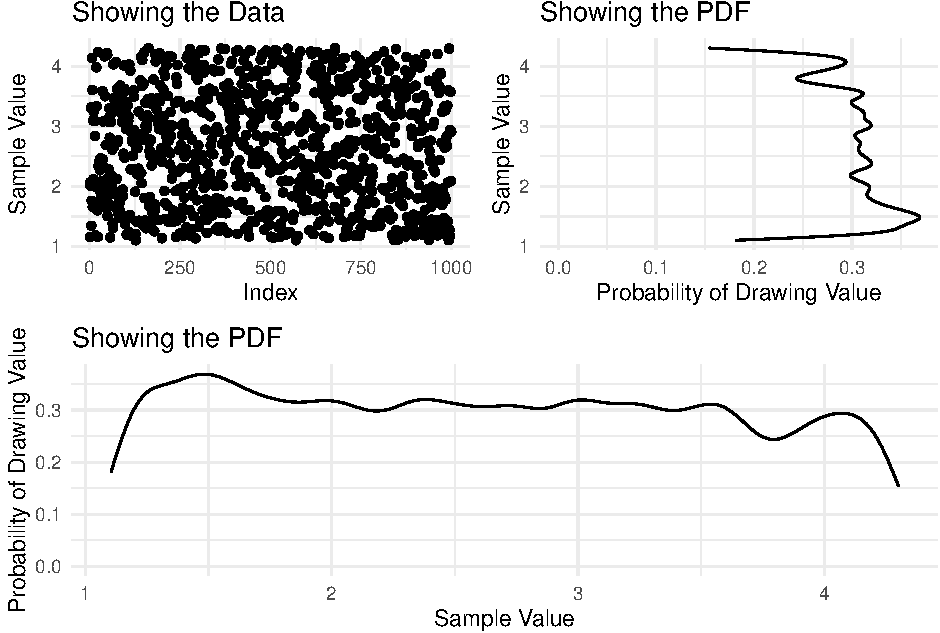
\includegraphics{02-random-variables_files/figure-pdf/plot uniform samples-1.pdf}

Interesting. From what we can see here, there does not appear to be any
discernible pattern. This leaves us with two options: either, we might
reduce the resolution that we're using to view this pattern, or we might
take more samples and hold the resolution constant. Below, two different
plots show these differing approaches, and are \emph{very} explicit
about the code that creates them.

\begin{Shaded}
\begin{Highlighting}[]
\NormalTok{samples\_uniform\_moar }\OtherTok{\textless{}{-}} \FunctionTok{runif}\NormalTok{(}\AttributeTok{n =} \DecValTok{1000000}\NormalTok{, }\AttributeTok{min =} \FloatTok{1.1}\NormalTok{, }\AttributeTok{max =} \FloatTok{4.3}\NormalTok{)}
\end{Highlighting}
\end{Shaded}

\begin{Shaded}
\begin{Highlighting}[]
\NormalTok{plot\_low\_res }\OtherTok{\textless{}{-}} \FunctionTok{ggplot}\NormalTok{()   }\SpecialCharTok{+} 
  \FunctionTok{aes}\NormalTok{(}\AttributeTok{x =}\NormalTok{ samples\_uniform) }\SpecialCharTok{+} 
  \FunctionTok{geom\_density}\NormalTok{(}\AttributeTok{bw =} \FloatTok{0.1}\NormalTok{)   }\SpecialCharTok{+} 
  \FunctionTok{lims}\NormalTok{(}\AttributeTok{y =} \FunctionTok{c}\NormalTok{(}\DecValTok{0}\NormalTok{,}\FloatTok{0.4}\NormalTok{))       }\SpecialCharTok{+} 
  \FunctionTok{labs}\NormalTok{(}\AttributeTok{title =} \StringTok{\textquotesingle{}Low Res, Low Data\textquotesingle{}}\NormalTok{)}

\NormalTok{plot\_high\_res }\OtherTok{\textless{}{-}} \FunctionTok{ggplot}\NormalTok{()       }\SpecialCharTok{+} 
  \FunctionTok{aes}\NormalTok{(}\AttributeTok{x =}\NormalTok{ samples\_uniform\_moar) }\SpecialCharTok{+} 
  \FunctionTok{geom\_density}\NormalTok{(}\AttributeTok{bw =} \FloatTok{0.01}\NormalTok{)       }\SpecialCharTok{+} 
  \FunctionTok{lims}\NormalTok{(}\AttributeTok{y =} \FunctionTok{c}\NormalTok{(}\DecValTok{0}\NormalTok{,}\FloatTok{0.4}\NormalTok{))            }\SpecialCharTok{+} 
  \FunctionTok{labs}\NormalTok{(}\AttributeTok{title =} \StringTok{\textquotesingle{}High Res, More Data\textquotesingle{}}\NormalTok{)}

\NormalTok{plot\_low\_res }\SpecialCharTok{|}\NormalTok{ plot\_high\_res}
\end{Highlighting}
\end{Shaded}

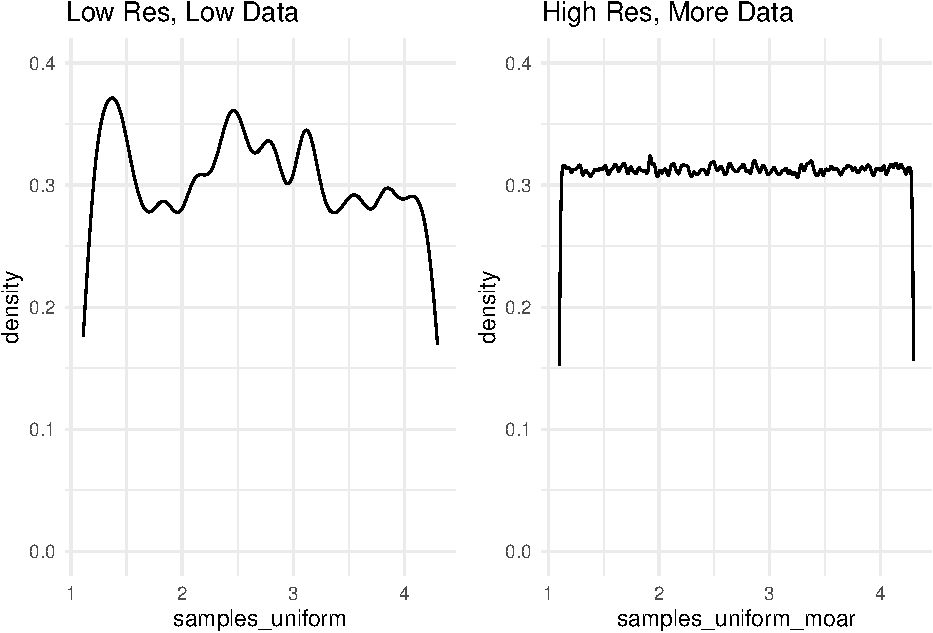
\includegraphics{02-random-variables_files/figure-pdf/plot uniform distributions-1.pdf}

\subsection{Example: The Normal
Distribution}\label{example-the-normal-distribution}

Folks might have some prior beliefs about the Normal distribution. Don't
worry, we'll cover this later in the course. But, this is the
distribution that you have in mind when you're thinking of a ``bell
curve''.

We can use the same method to visualize a normal distribution as we did
for a uniform distribution. In this case, we would issue the call
\texttt{rnorm}, together with the population parameters that define the
population. At this point in the course, we do not expect that you will
know these (and, actually memorizing these facts are not a core focus of
the course), but you can
\href{https://en.wikipedia.org/wiki/Normal_distribution}{look them up}
if you like. Truthfully, statistics wikipedia is \emph{very} good.

Do do you notice anything about the \texttt{runif} and the
\texttt{rnorm} calls that we have identified? Both seem to name the
distribution: \(unif \approx uniform\) and \(norm \approx normal\), but
prepened with a \texttt{r}? This is for ``random draw''.

Base R is loaded with a \emph{pile} of basic statistics distributions,
which you can look into using \texttt{?distributions}.

\begin{Shaded}
\begin{Highlighting}[]
\NormalTok{samples\_normal }\OtherTok{\textless{}{-}} \FunctionTok{rnorm}\NormalTok{(}\AttributeTok{n =} \DecValTok{100000}\NormalTok{, }\AttributeTok{mean =} \DecValTok{18}\NormalTok{, }\AttributeTok{sd =} \DecValTok{4}\NormalTok{)}
\end{Highlighting}
\end{Shaded}

Like before, we could look at the first \(20\) of these samples.

\begin{Shaded}
\begin{Highlighting}[]
\NormalTok{samples\_normal[}\DecValTok{1}\SpecialCharTok{:}\DecValTok{20}\NormalTok{]}
\end{Highlighting}
\end{Shaded}

\begin{verbatim}
 [1] 20.01714 12.06071 18.98264 22.95449 14.66461 16.66013 21.63034 17.68357
 [9] 20.81829 16.47933 20.43985 17.37152 13.74835 18.17729 19.21103 23.63705
[17] 26.01543 15.64904 18.20650 19.18236
\end{verbatim}

And, from here we could visualize this distribution.

\begin{Shaded}
\begin{Highlighting}[]
\FunctionTok{ggplot}\NormalTok{() }\SpecialCharTok{+} 
  \FunctionTok{aes}\NormalTok{(}\AttributeTok{x =}\NormalTok{ samples\_normal) }\SpecialCharTok{+} 
  \FunctionTok{geom\_density}\NormalTok{() }\SpecialCharTok{+} 
  \FunctionTok{labs}\NormalTok{(}\AttributeTok{title =} \StringTok{\textquotesingle{}Visualization of this Normal Distribution\textquotesingle{}}\NormalTok{)}
\end{Highlighting}
\end{Shaded}

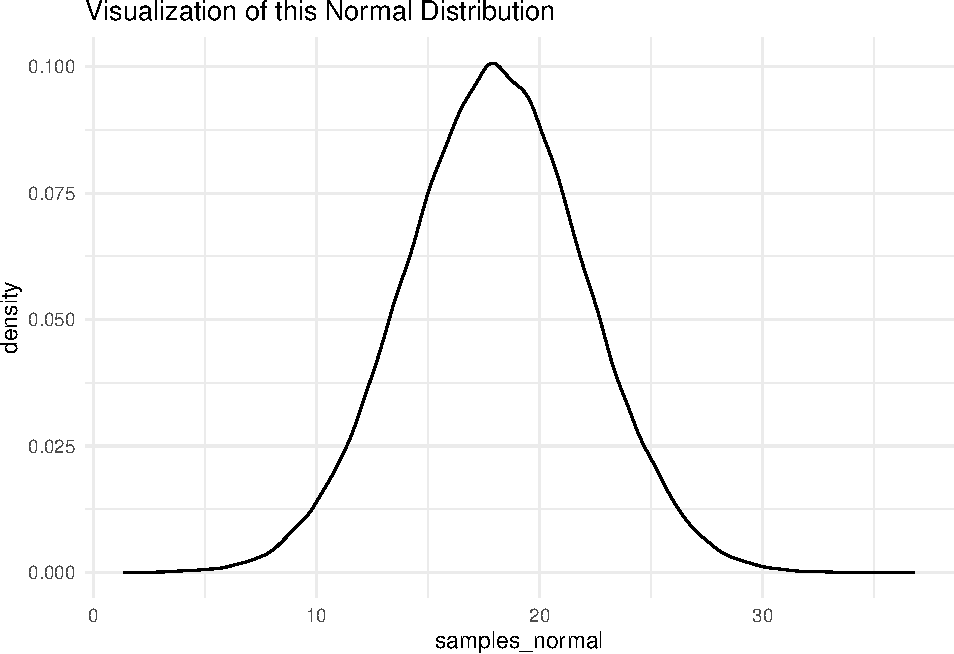
\includegraphics{02-random-variables_files/figure-pdf/plot normal-1.pdf}

\subsubsection{Combining This Ability}\label{combining-this-ability}

Consider three random variables \(A, B, C\). Suppose,

\[
\begin{aligned}    
  A & \sim Uniform(min=1.1, max=4.3) \\     
  B & \sim Normal(mean=18, sd=4)     \\     
  C &= A + B  \end{aligned}
\]

And, suppose that \(B\) is a random variable that is described by the
normal density that we considered earlier. Suppose that \(A\) and \(B\)
are independent of each other.

Finally, suppose that \(C = A + 2B\).

What does \(C\) look like?

Although this is a simple function applied to a random variable -- a
legal move -- the math would be tedious. What if, instead, one used this
simulation method to get a sense for the distribution?

\begin{Shaded}
\begin{Highlighting}[]
\NormalTok{samples\_A }\OtherTok{\textless{}{-}} \FunctionTok{runif}\NormalTok{(}\AttributeTok{n =} \DecValTok{10000}\NormalTok{, }\AttributeTok{min =} \FloatTok{1.1}\NormalTok{, }\AttributeTok{max =} \FloatTok{4.3}\NormalTok{)}
\NormalTok{samples\_B }\OtherTok{\textless{}{-}} \FunctionTok{rnorm}\NormalTok{(}\AttributeTok{n =} \DecValTok{10000}\NormalTok{, }\AttributeTok{mean =} \DecValTok{18}\NormalTok{, }\AttributeTok{sd =} \DecValTok{4}\NormalTok{)}

\NormalTok{samples\_C }\OtherTok{\textless{}{-}}\NormalTok{ samples\_A }\SpecialCharTok{+}\NormalTok{ samples\_B}
\end{Highlighting}
\end{Shaded}

\begin{Shaded}
\begin{Highlighting}[]
\NormalTok{plot\_C }\OtherTok{\textless{}{-}} \FunctionTok{ggplot}\NormalTok{() }\SpecialCharTok{+} 
  \FunctionTok{aes}\NormalTok{(}\AttributeTok{x =}\NormalTok{ samples\_C) }\SpecialCharTok{+} 
  \FunctionTok{geom\_density}\NormalTok{()}

\NormalTok{plot\_C\_and\_A\_and\_B }\OtherTok{\textless{}{-}} \FunctionTok{ggplot}\NormalTok{()   }\SpecialCharTok{+} 
  \FunctionTok{geom\_density}\NormalTok{(}\FunctionTok{aes}\NormalTok{(}\AttributeTok{x =}\NormalTok{ samples\_A), }\AttributeTok{color =} \StringTok{\textquotesingle{}\#003262\textquotesingle{}}\NormalTok{) }\SpecialCharTok{+} 
  \FunctionTok{geom\_density}\NormalTok{(}\FunctionTok{aes}\NormalTok{(}\AttributeTok{x =}\NormalTok{ samples\_B), }\AttributeTok{color =} \StringTok{\textquotesingle{}\#FDB515\textquotesingle{}}\NormalTok{) }\SpecialCharTok{+} 
  \FunctionTok{geom\_density}\NormalTok{(}\FunctionTok{aes}\NormalTok{(}\AttributeTok{x =}\NormalTok{ samples\_C), }\AttributeTok{color =} \StringTok{\textquotesingle{}darkred\textquotesingle{}}\NormalTok{)}

\NormalTok{plot\_C\_and\_A\_and\_B}
\end{Highlighting}
\end{Shaded}

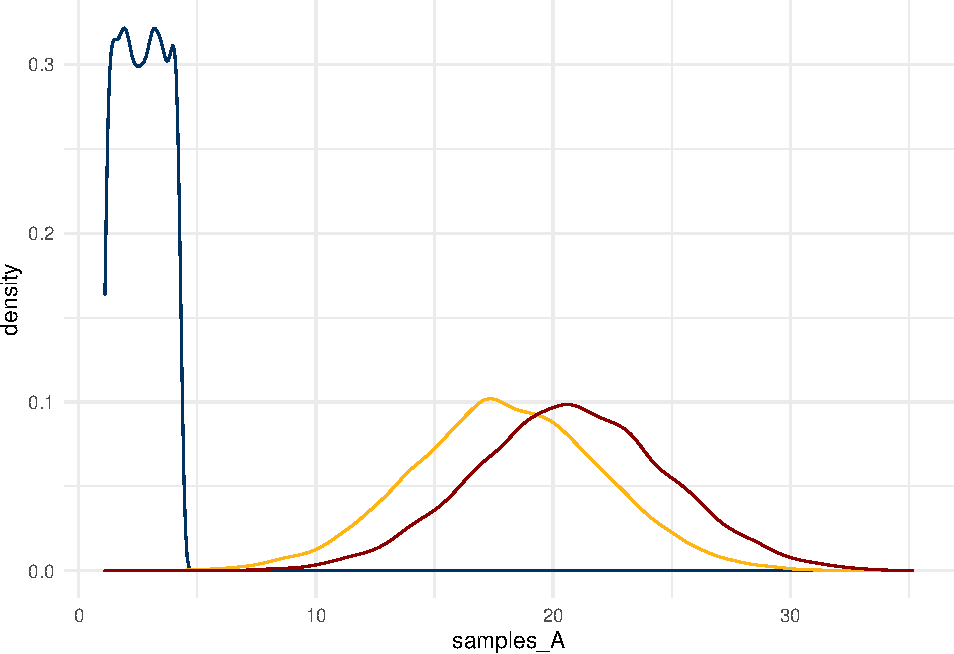
\includegraphics{02-random-variables_files/figure-pdf/plot C-1.pdf}

\section{Review of Terms}\label{review-of-terms}

Remember some of the key terms we learned in the async:

\begin{itemize}
\tightlist
\item
  Joint Density Function
\item
  Conditional Distribution
\item
  Marginal Distribution
\end{itemize}

\chapter{Summarizing Distributions}\label{summarizing-distributions}

\begin{figure}[H]

{\centering \includegraphics{./images/yosemite.jpg}

}

\caption{a majestic valley}

\end{figure}%

In the last live session, we introduced random variables; probability
density and cumulative density; and, made the connection between joint,
marginal, and conditional distributions. All of these concepts work with
the \textbf{entire} distribution.

Take, for example, the idea of conditional probability. We noted that
conditional probability is defined to be:

\[
  f_{Y|X}(y|x) = \frac{f_{Y,X}(y,x)}{f_{X}(x)}
\]

This is a powerful concept that shows a lot of the range of the
reasoning system that we've built to this point! The probability
distribution of \(Y\) might change as a result of changes in \(X\). If
you unpack that just a little bit more, we might say that
\(f_{Y|X}(y|x)\) -- the probability density of \(Y\) -- which is itself
a function, is \emph{also} a function of \(X\). To say it again, to be
very explicit: the function is a function of another input. That might
sound wild, but it is all perfectly consistent with the world that we've
built to this point.

This concept is \textbf{very} expressive. Knowing \(f_{Y}(y)\) gives a
full information representation of a variable; knowing \(f_{Y|X}(y|x)\)
lets you update that information to make an even more informative
statement about \(Y\). In \emph{Foundations} and at this point in the
class, we deal only with conditional probability conditioning on a
single variable, but the process generalizes.

For example, if there were four random variables, \(A, B, C, D\), we
could make a statement about \(A\) that conditions on \(B, C, D\):

\[
  f_{A|\{B,C,D\}}(a|\{b,c,d\}) = \frac{f_{A,B,C,D}(a,b,c,d)}{f_{B,C,D}(b,c,d)}
\]

In this week's materials we are going to go in the \emph{opposite}
direction: Rather than producing a very expressive system of
probabilities, we're going to attempt to summarize all of the
information contained in a pdf into lower-dimensional representations.
Our first task will be summarizing a single random variable in two ways:

\begin{enumerate}
\def\labelenumi{\arabic{enumi}.}
\tightlist
\item
  Where is the ``center'' of the random variable; and,
\item
  How dispersed, ``on average'' is the random variable from this center.
\end{enumerate}

After developing the concepts of \emph{expectation} and \emph{variance}
(which are 1 \& 2 above, respectively), we will develop a summary of a
joint distribution: the \emph{covariance}. The particular definitions
that we choose to call expectation, variance, and covariance require
justification. Why should we use these \emph{particular} formulae as
measures of the ``center'' and ``dispersion''?

We ground these summaries in the \textbf{Mean Squared Error} evaluative
metric, as well as justifying this metric.

\section{Learning Objectives}\label{learning-objectives-2}

At the end of the live session and homework this week, students will be
able to:

\begin{enumerate}
\def\labelenumi{\arabic{enumi}.}
\tightlist
\item
  \textbf{Understand} the importance of thinking in terms of random
  variables, while;
\item
  Being able to \textbf{appreciate} that it is not typically possible to
  fully model the world with a single function.
\item
  \textbf{Articulate} why we need a target for a model, and propose
  several possible such targets.
\item
  \textbf{Justify} why expectation is a good model, why variance is a
  reasonable model, and how covariance relates two-random variables with
  a common joint distribution.
\item
  \textbf{Produce} summaries of location and relationship given a
  particular functional form for a random variable.
\end{enumerate}

\section{Class Announcements}\label{class-announcements-1}

Where have we come from, and where are we going?

\subsection{What is in the rearview
mirror?}\label{what-is-in-the-rearview-mirror}

\begin{itemize}
\tightlist
\item
  Statisticians create a population model to represent the world; random
  variables are the building blocks of such a model.
\item
  We can describe the distribution of a random variable using:

  \begin{itemize}
  \tightlist
  \item
    A \emph{CDF} for all random variables
  \item
    A \emph{PMF} for discrete random variables
  \item
    A \emph{PDF} for continuous random variables
  \end{itemize}
\item
  When we have multiple random variables,

  \begin{itemize}
  \tightlist
  \item
    The joint PMF/PDF describes how they behave together
  \item
    The marginal PMF/PDF describes one variable in isolation
  \item
    The conditional PMF/PDF describes one variable given the value of
    another
  \end{itemize}
\end{itemize}

\subsection{Today's Lesson}\label{todays-lesson}

What might seem frustrating about this probability theory system of
reasoning is that we are building a castle in the sky -- a fiction.
We're supposing that there is some function that describes the
probability that values are generated. In reality, there is no such
generative function; it is \emph{extremely unlikely} (though we'll
acknowledge that it is possible) that the physical reality we believe we
exist within is just a complex simulation that has been programmed with
functions by some unknown designer.

Especially frustrating is that we're supposing this function, and then
we're further saying,

\begin{quote}
``If only we had this impossible function; and if only we also had the
ability to take an impossible derivative of this impossible function,
then we could\ldots{}''
\end{quote}

\subsubsection{Single number summaries of a single random
variable}\label{single-number-summaries-of-a-single-random-variable}

But, here's the upshot!

\textbf{What we are doing today is laying the baseline for models that
we will introduce next week.} Here, we are going to suggest that there
are radical simplifications that we can produce that hold specific
guarantees, no matter how complex the function that we're reasoning
about.

In particular, in one specific usage of the term \emph{best} we will
prove that the Expectation operation is the best one-number summary of
any distribution. To do so, we will define a term, \emph{variance},
which is the squared deviations from the expectation of a variable that
describes how ``spread out'' is a variable. Then, we will define a
concept that is the \emph{mean squared error} that is the square of the
distance between a model prediction and a random variable's realization.
The key realization is that when the model predicts the expectation,
then the MSE is equal to the variance of the random variable, which is
the smallest possible value it could realize.

\subsubsection{Single number summaries of relationships between random
variables}\label{single-number-summaries-of-relationships-between-random-variables}

Although the single number summaries are \textbf{incredibly} powerful,
that's not enough for today's lesson! We're also going to suggest that
we can create a measure of linear dependence between two variables that
we call the ``covariance'', and a related, re-scaled version of this
relationship that is called the correlation.

\subsection{Future Attractions}\label{future-attractions}

\begin{itemize}
\tightlist
\item
  A predictor is a function that provides a value for one variable,
  given values of some others.
\item
  Using our summary tools, we will define a predictor's error and then
  minimize it.
\item
  This is a basis for linear regression
\end{itemize}

\section{Discussion of Terms}\label{discussion-of-terms}

\subsection{Expected Value}\label{expected-value}

We define the expected value to be the following for a continuous random
variable:

\section{Expected Value}\label{expected-value-1}

For a continuous random variable \(X\) with PDF \(f\), the
\emph{expected value} of \(X\), written \(E[X]\) is

\[
E[X] = \int_{-\infty}^{\infty}xf_{X}(x) dx
\]

Oh, ok. If you say so. (We do\ldots).

There are two really important things to grasp here:

\begin{enumerate}
\def\labelenumi{\arabic{enumi}.}
\tightlist
\item
  What does this mean about a particular PDF?
\item
  What is the justification for this \emph{particualar} definition?
\end{enumerate}

With your instructor, talk about what each of the following definitions
mean in your own words. For key concepts, you might also formalize this
intuition into a formula that can be computed.

\begin{itemize}
\tightlist
\item
  Expected Value, or Expectation
\item
  Central Moments \(\rightarrow\) Variance \(\rightarrow\) Standard
  Deviation
\item
  Set aside for later: Chebyshev's Inequality and the Normal
  Distribution
\item
  Mean Squared Error and its alternative formula
\item
  Covariance and Correlation
\end{itemize}

\section{Computing Examples}\label{computing-examples}

\subsection{Expected Value of Education {[}discrete random
variable{]}}\label{expected-value-of-education-discrete-random-variable}

\begin{itemize}
\tightlist
\item
  The expected value of a discrete random variable \(X\) is the weighted
  average of the values in the range of \(X\).
\item
  Suppose that \(X\) represents the number of years of education that
  someone has completed, and so has a support that ranges from \(0\)
  years of education, up to \(28\) years of education. (Incidentally,
  Mark Labovitz has about 28 years of education.)
\item
  You can then think of
\end{itemize}

\includegraphics{03-summarizing-distributions_files/figure-pdf/unnamed-chunk-1-1.pdf}

\begin{itemize}
\tightlist
\item
  Without using specific numbers, describe the process you would use to
  calculate the expected value of this distribution.
\end{itemize}

\subsection{Using a formula}\label{using-a-formula}

\begin{itemize}
\tightlist
\item
  Does the following formula match with your intuitive description of
  the \emph{expected value}? Why, or why not?
\end{itemize}

{[}

\begin{aligned}
  E[X] &= \sum_{x \in \{EDU\}} x \cdot f(x) \\ 
       &= \sum_{x=0}^{x=28} x\cdot P(X=x)
  \end{aligned}

{]}

\section{Computing by Hand}\label{computing-by-hand}

\subsection{Compute the Expected
Value}\label{compute-the-expected-value}

Let \(X\) represent the result of one roll of a 6 sided die where the
events \(\omega \in \Omega\) are mapped using a straightforward
function: \(X(\omega):\) is a function that counts the number of spots
that are showing, and maps the number of dots to the corresponding
integer, \(\mathbb{Z}\).

\begin{itemize}
\tightlist
\item
  Calculating by hand, what is the expected value \(X\), which we write
  as \(E[X]\)?
\item
  After you have calculated \(E[X]\): Is it possible that the result of
  a roll is this value?
\end{itemize}

\begin{Shaded}
\begin{Highlighting}[]
\FunctionTok{blank\_lines}\NormalTok{(}\DecValTok{20}\NormalTok{)}
\end{Highlighting}
\end{Shaded}

\vspace{20cm}

\subsection{Playing a Gnome Game, Part
1}\label{playing-a-gnome-game-part-1}

\begin{itemize}
\tightlist
\item
  Suppose that, out on a hike in the hills above campus, you happen
  across a gnome who asks you if you would like to play the following
  game:

  \begin{itemize}
  \tightlist
  \item
    You pay the gnome a dollar, and guess a number between 0 and 6. So,
    let \(g \in \mathbb{R}: 0 \leq g \leq 6\).
  \item
    After you make your guess, the gnome rolls a dice, which comes up
    with a value \(d \in \mathbb{Z}: d \in \{1,2,3,4,5,6\}\).
  \item
    The gnome pays you \(p = 0.25 \times |d - g|\).
  \item
    \textbf{First question}: What is the best guess you can make?
  \item
    \textbf{Second Question}: Should you play this game?
  \end{itemize}
\end{itemize}

\begin{quote}
Fill this in by hand.
\end{quote}

\begin{Shaded}
\begin{Highlighting}[]
\FunctionTok{blank\_lines}\NormalTok{(}\DecValTok{20}\NormalTok{)}
\end{Highlighting}
\end{Shaded}

\vspace{20cm}

\subsection{Compute the Variance}\label{compute-the-variance}

Let \(X\) represent the result of one roll of a 6 sided die.

\begin{itemize}
\tightlist
\item
  Calculating by hand, what is the variance of \(X\)?
\end{itemize}

\begin{Shaded}
\begin{Highlighting}[]
\FunctionTok{blank\_lines}\NormalTok{(}\DecValTok{20}\NormalTok{)}
\end{Highlighting}
\end{Shaded}

\vspace{20cm}

\subsection{Playing a Gnome Game, Part
2}\label{playing-a-gnome-game-part-2}

\begin{itemize}
\tightlist
\item
  How much do you expect to make on any particular time that you play
  the game with the best strategy?
\end{itemize}

\begin{Shaded}
\begin{Highlighting}[]
\FunctionTok{blank\_lines}\NormalTok{(}\DecValTok{20}\NormalTok{)}
\end{Highlighting}
\end{Shaded}

\vspace{20cm}

\section{Expected Value by Code}\label{expected-value-by-code}

\subsection{Expected Value of a Six-Sided
Die}\label{expected-value-of-a-six-sided-die}

Let \(X\) represent the result of one roll of a 6 sided die.

\begin{itemize}
\tightlist
\item
  Build an object to represent the whole sample space, \(\Omega\) of a
  six sided die.
\item
  Determine what probabilities to assign to each value of that object.
\item
  Write the code to run the expectation algorithm that you just
  performed by hand.
\end{itemize}

\begin{Shaded}
\begin{Highlighting}[]
\NormalTok{die }\OtherTok{\textless{}{-}} \FunctionTok{data.frame}\NormalTok{(}
  \AttributeTok{value =} \StringTok{\textquotesingle{}fill this in\textquotesingle{}}\NormalTok{,}
  \AttributeTok{prob  =} \StringTok{\textquotesingle{}fill this in\textquotesingle{}}
\NormalTok{)}
\end{Highlighting}
\end{Shaded}

\subsection{Variance of a Six-Sided
Die}\label{variance-of-a-six-sided-die}

Let \(X\) represent the result of one roll of a 6 sided die. Using what
you know about the definition of variance, write a function that will
compute the variance of your \texttt{die} object.

\begin{Shaded}
\begin{Highlighting}[]
\NormalTok{variance\_function }\OtherTok{\textless{}{-}} \ControlFlowTok{function}\NormalTok{(die) \{ }
  \DocumentationTok{\#\# fill this in}
\NormalTok{  mu }\OtherTok{=} \StringTok{\textquotesingle{}fill this in\textquotesingle{}}   \DocumentationTok{\#\# you should index to the correct column}
\NormalTok{  var }\OtherTok{=} \StringTok{\textquotesingle{}fill this in\textquotesingle{}}  \DocumentationTok{\#\# for each, and use the correct function}
  
  \FunctionTok{return}\NormalTok{(var)}
\NormalTok{\}}

\FunctionTok{variance\_function}\NormalTok{(die)}
\end{Highlighting}
\end{Shaded}

\begin{verbatim}
[1] "fill this in"
\end{verbatim}

Suppose that you had to keep the values the same on the die (that is the
domain of the outcome still had to be the countable set of integers from
one to six), but that you could modify the actual random process. Maybe
you could sand off some of the corners on the die, or you could place
weights on one side so that the side is less likely to come up. In this
case, \(\omega \in \{1,2,3,4,5,6\}\), but you're able to make a new
\(f_{D}(d)\).

\begin{itemize}
\tightlist
\item
  How would you change the probability distribution to decrease the
  variance of this random variable?
\item
  What is the smallest value that you can generate for this random
  variable? Use the \texttt{variance\_function} from above to actually
  compute this variance.
\item
  What is the largest value of variance that you can generate for this
  random variable? Use the \texttt{variance\_function} from above to
  actually compute this variance.
\end{itemize}

Now suppose that you again had an equal probability of every outcome,
but you were to apply a function to the number of spots that are showing
on the die. Rather that each dot contributing one value to the random
variable, instead the random variable's outcome is the square of the
number of spots.

\begin{itemize}
\tightlist
\item
  How would this change the mean?
\item
  How would this change the variance?
\end{itemize}

\section{Practice Computing}\label{practice-computing}

\subsection{Single Variable}\label{single-variable}

Suppose that \(X\) has the following density function:

\[
  f_{X}(x) = \begin{cases} 
    6x(1 - x), & 0 < x < 1 \\ 
    0, & otherwise \\ 
  \end{cases}
\]

\begin{itemize}
\tightlist
\item
  Find \(E[X]\).
\item
  Find \(E[X^2]\).
\item
  Find \(V[X]\).
\end{itemize}

\subsection{Joint Density}\label{joint-density-1}

\subsubsection{Discrete Case: Calculate
Covariance}\label{discrete-case-calculate-covariance}

In the reading, you saw that we define \textbf{covariance} to be:

\[
\begin{aligned}
Cov[X,Y]    &= E[(E[X] - X)^{2}(E[Y] - Y)^{2}] \\ 
            &= E[XY] - E[X]E[Y]
\end{aligned} 
\]

And, \textbf{correlation} to be a rescaled version of \emph{covariance}:

\[
\begin{aligned}
Cor[X,Y]    & \equiv \rho[X,Y] \\ 
            & = \frac{Cov[X,Y]}{\sigma_{X}\sigma_{Y}} \\
\end{aligned}            
\]

Suppose that \(X\) and \(Y\) are discrete random variables, where \(X\)
represents number of office hours attended, and \(Y\) represents owning
a cat. Furthermore, suppose that \(X\) and \(Y\) have the joint pmf,

\begin{longtable}[]{@{}lcc@{}}
\toprule\noalign{}
f(x,y) & y=0 & y=1 \\
\midrule\noalign{}
\endhead
\bottomrule\noalign{}
\endlastfoot
x=0 & 0.10 & 0.35 \\
x=1 & 0.05 & 0.05 \\
x=2 & 0.10 & 0.35 \\
\end{longtable}

\begin{enumerate}
\def\labelenumi{\arabic{enumi}.}
\tightlist
\item
  Calculate the covariance of \(X\) and \(Y\).
\item
  Are X and Y independent? Why or why not?
\end{enumerate}

\subsubsection{Continuous Case: Calculate
Covariance}\label{continuous-case-calculate-covariance}

Suppose that \(X\) and \(Y\) have joint density
\(f_{X,Y}(x,y) = 8xy, 0 \leq y < x \leq 1.\)

\begin{itemize}
\tightlist
\item
  Break into groups to find \(\operatorname{Cov}[X,Y]\)
\end{itemize}

Suppose that \(X\) and \(Y\) are random variables with joint density

\[
f_{X,Y}(x,y) = 
\begin{cases} 
 1, & -y < x < y, 0 < y < 1 \\ 
 0, & \textrm{elsewhere}
\end{cases}
\]

Show that \(\operatorname{Cov}[X,Y] = 0\) but that \(X\) and \(Y\) are
dependent.

\section{Write Code}\label{write-code}

Suppose that you have a random variable with a \textbf{gnarly}
probability distribution function:

\[ 
  f_{X}(x) = \frac{3*\left(x - 2x^2 + x^3\right)}{2}, 0\leq x\leq 2
\]

If you had to pick a single value that minimizes the \(MSE\) of this
function, what would it be?

\begin{itemize}
\tightlist
\item
  First, how would you approach this problem \emph{analytically}. By
  this, we mean, ``how would you solve this with the closed form answer?
\item
  Second, how might you approach this problem \emph{computationally}. By
  this, we mean, ``how might you write code that would produce a numeric
  approximation of the closed form solution?'' Don't worry about
  actually writing the code -- we'll have done that for you, but what is
  the \emph{process} (called in our world, \emph{algorithm}) that you
  would use to determine the value that produces the smallest \(MSE\)?
\end{itemize}

\begin{Shaded}
\begin{Highlighting}[]
\NormalTok{pdf\_fun }\OtherTok{\textless{}{-}} \ControlFlowTok{function}\NormalTok{(x) \{ }
\NormalTok{  (}\DecValTok{3}\SpecialCharTok{/}\DecValTok{2}\NormalTok{)}\SpecialCharTok{*}\NormalTok{(x }\SpecialCharTok{{-}}\NormalTok{ (}\DecValTok{2}\SpecialCharTok{*}\NormalTok{x}\SpecialCharTok{\^{}}\DecValTok{2}\NormalTok{) }\SpecialCharTok{+}\NormalTok{ x}\SpecialCharTok{\^{}}\DecValTok{3}\NormalTok{)}
\NormalTok{\}}
\end{Highlighting}
\end{Shaded}

\begin{Shaded}
\begin{Highlighting}[]
\NormalTok{support }\OtherTok{\textless{}{-}} \FunctionTok{seq}\NormalTok{(}\AttributeTok{from=}\DecValTok{0}\NormalTok{, }\AttributeTok{to=}\DecValTok{2}\NormalTok{, }\AttributeTok{by=}\FloatTok{0.01}\NormalTok{)}
\end{Highlighting}
\end{Shaded}

\begin{Shaded}
\begin{Highlighting}[]
\FunctionTok{ggplot}\NormalTok{() }\SpecialCharTok{+} 
  \FunctionTok{geom\_function}\NormalTok{(}\AttributeTok{fun =}\NormalTok{ pdf\_fun) }\SpecialCharTok{+} 
  \FunctionTok{xlim}\NormalTok{(}\FunctionTok{min}\NormalTok{(support), }\FunctionTok{max}\NormalTok{(support)) }\SpecialCharTok{+} 
  \FunctionTok{labs}\NormalTok{(}
    \AttributeTok{title =} \StringTok{"A Gnarly Plot"}
\NormalTok{  )}
\end{Highlighting}
\end{Shaded}

\includegraphics{03-summarizing-distributions_files/figure-pdf/unnamed-chunk-10-1.pdf}

\begin{Shaded}
\begin{Highlighting}[]
\NormalTok{expected\_value }\OtherTok{\textless{}{-}} \ControlFlowTok{function}\NormalTok{(value, prob)\{}
  \FunctionTok{sum}\NormalTok{(value }\SpecialCharTok{*}\NormalTok{ prob)}
\NormalTok{\}}

\NormalTok{mse }\OtherTok{\textless{}{-}} \ControlFlowTok{function}\NormalTok{(c) \{ }
  \FunctionTok{expected\_value}\NormalTok{(}
    \AttributeTok{value =}\NormalTok{ (support }\SpecialCharTok{{-}}\NormalTok{ c)}\SpecialCharTok{\^{}}\DecValTok{2}\NormalTok{, }
    \AttributeTok{prob  =} \FunctionTok{pdf\_fun}\NormalTok{(support)}
\NormalTok{  )  }
\NormalTok{\}}

\NormalTok{mpe }\OtherTok{\textless{}{-}} \ControlFlowTok{function}\NormalTok{(c, power) \{ }
  \FunctionTok{expected\_value}\NormalTok{(}
    \AttributeTok{value =}\NormalTok{ (support }\SpecialCharTok{{-}}\NormalTok{ c)}\SpecialCharTok{\^{}}\NormalTok{power, }
    \AttributeTok{prob  =} \FunctionTok{pdf\_fun}\NormalTok{(support)}
\NormalTok{  )}
\NormalTok{\}}
\end{Highlighting}
\end{Shaded}

\begin{Shaded}
\begin{Highlighting}[]
\NormalTok{mean\_absolute\_error }\OtherTok{\textless{}{-}} \ControlFlowTok{function}\NormalTok{(c) \{ }
\NormalTok{  x\_values }\OtherTok{\textless{}{-}} \FunctionTok{pdf\_fun}\NormalTok{(support)}
\NormalTok{  mae\_     }\OtherTok{\textless{}{-}} \FunctionTok{mean}\NormalTok{(}\FunctionTok{abs}\NormalTok{(x\_values }\SpecialCharTok{{-}}\NormalTok{ c))}
\NormalTok{\}}

\NormalTok{mean\_square\_error }\OtherTok{\textless{}{-}} \ControlFlowTok{function}\NormalTok{(c) \{ }
\NormalTok{  x\_values }\OtherTok{\textless{}{-}} \FunctionTok{pdf\_fun}\NormalTok{(support)}
\NormalTok{  mse\_     }\OtherTok{\textless{}{-}} \FunctionTok{sum}\NormalTok{(((x\_values }\SpecialCharTok{{-}}\NormalTok{ c)}\SpecialCharTok{\^{}}\DecValTok{2}\NormalTok{) }\SpecialCharTok{*}\NormalTok{ x\_values)}
  \FunctionTok{return}\NormalTok{(mse\_)}
\NormalTok{\}}

\NormalTok{mean\_cubic\_error }\OtherTok{\textless{}{-}} \ControlFlowTok{function}\NormalTok{(c) \{ }
\NormalTok{  x\_values }\OtherTok{\textless{}{-}} \FunctionTok{pdf\_fun}\NormalTok{(support) }
\NormalTok{  mce\_     }\OtherTok{\textless{}{-}} \FunctionTok{mean}\NormalTok{((x\_values }\SpecialCharTok{{-}}\NormalTok{ c)}\SpecialCharTok{\^{}}\DecValTok{3}\NormalTok{)}
\NormalTok{\}}

\NormalTok{mean\_quadratic\_error }\OtherTok{\textless{}{-}} \ControlFlowTok{function}\NormalTok{(c) \{ }
\NormalTok{  x\_values }\OtherTok{\textless{}{-}} \FunctionTok{pdf\_fun}\NormalTok{(support)}
\NormalTok{  mqe\_     }\OtherTok{\textless{}{-}} \FunctionTok{mean}\NormalTok{((x\_values }\SpecialCharTok{{-}}\NormalTok{ c)}\SpecialCharTok{\^{}}\DecValTok{4}\NormalTok{)}
  \FunctionTok{return}\NormalTok{(mqe\_)}
\NormalTok{\}}

\NormalTok{mean\_power\_error }\OtherTok{\textless{}{-}} \ControlFlowTok{function}\NormalTok{(c, power) \{ }
\NormalTok{  x\_values }\OtherTok{\textless{}{-}} \FunctionTok{pdf\_fun}\NormalTok{(support)}
\NormalTok{  m\_power\_e\_     }\OtherTok{\textless{}{-}} \FunctionTok{mean}\NormalTok{((x\_values }\SpecialCharTok{{-}}\NormalTok{ c)}\SpecialCharTok{\^{}}\NormalTok{power)}
  \FunctionTok{return}\NormalTok{(m\_power\_e\_)}
\NormalTok{\}}
\end{Highlighting}
\end{Shaded}

\begin{Shaded}
\begin{Highlighting}[]
\NormalTok{mean\_absolute\_error  }\OtherTok{\textless{}{-}} \FunctionTok{Vectorize}\NormalTok{(mean\_absolute\_error)}
\NormalTok{mean\_square\_error    }\OtherTok{\textless{}{-}} \FunctionTok{Vectorize}\NormalTok{(mean\_square\_error)}
\NormalTok{mean\_cubic\_error     }\OtherTok{\textless{}{-}} \FunctionTok{Vectorize}\NormalTok{(mean\_cubic\_error)}
\NormalTok{mean\_quadratic\_error }\OtherTok{\textless{}{-}} \FunctionTok{Vectorize}\NormalTok{(mean\_quadratic\_error)}
\NormalTok{mean\_power\_error     }\OtherTok{\textless{}{-}} \FunctionTok{Vectorize}\NormalTok{(mean\_power\_error)}
\end{Highlighting}
\end{Shaded}

\begin{Shaded}
\begin{Highlighting}[]
\NormalTok{mae\_ }\OtherTok{\textless{}{-}} \FunctionTok{mean\_absolute\_error}\NormalTok{(}
  \AttributeTok{c =}\NormalTok{ support}
\NormalTok{)}
\NormalTok{mse\_ }\OtherTok{\textless{}{-}} \FunctionTok{mean\_square\_error}\NormalTok{(}
  \AttributeTok{c =}\NormalTok{ support}
\NormalTok{  )}
\NormalTok{mce\_ }\OtherTok{\textless{}{-}} \FunctionTok{mean\_cubic\_error}\NormalTok{(}
  \AttributeTok{c =}\NormalTok{ support}
\NormalTok{)}
\NormalTok{mqe\_ }\OtherTok{\textless{}{-}} \FunctionTok{mean\_quadratic\_error}\NormalTok{(}
  \AttributeTok{c =}\NormalTok{ support}
\NormalTok{)}
\end{Highlighting}
\end{Shaded}

\begin{Shaded}
\begin{Highlighting}[]
\NormalTok{absolute\_error\_ }\OtherTok{\textless{}{-}} \FunctionTok{optim}\NormalTok{(}
  \AttributeTok{par =} \DecValTok{0}\NormalTok{, }
  \AttributeTok{fn =}\NormalTok{ mean\_absolute\_error, }
  \AttributeTok{method =} \StringTok{\textquotesingle{}Brent\textquotesingle{}}\NormalTok{, }
  \AttributeTok{lower =} \DecValTok{0}\NormalTok{, }\AttributeTok{upper =} \DecValTok{2}
\NormalTok{  )}\SpecialCharTok{$}\NormalTok{par}

\NormalTok{squared\_error\_ }\OtherTok{\textless{}{-}} \FunctionTok{optim}\NormalTok{(}
  \AttributeTok{par =} \DecValTok{0}\NormalTok{, }
  \AttributeTok{fn =}\NormalTok{ mean\_square\_error, }
  \AttributeTok{method =} \StringTok{"Brent"}\NormalTok{, }
  \AttributeTok{lower =} \DecValTok{0}\NormalTok{, }\AttributeTok{upper =} \DecValTok{2}
\NormalTok{  )}\SpecialCharTok{$}\NormalTok{par}
\NormalTok{cubic\_error\_ }\OtherTok{\textless{}{-}} \FunctionTok{optim}\NormalTok{(}
  \AttributeTok{par =} \DecValTok{0}\NormalTok{, }
  \AttributeTok{fn =}\NormalTok{ mean\_cubic\_error, }
  \AttributeTok{method =} \StringTok{"Brent"}\NormalTok{, }
  \AttributeTok{lower =} \DecValTok{0}\NormalTok{, }\AttributeTok{upper =} \DecValTok{2}
\NormalTok{  )}\SpecialCharTok{$}\NormalTok{par}
\NormalTok{quadratic\_error\_ }\OtherTok{\textless{}{-}} \FunctionTok{optim}\NormalTok{(}
  \AttributeTok{par =} \DecValTok{0}\NormalTok{, }
  \AttributeTok{fn =}\NormalTok{ mean\_quadratic\_error, }
  \AttributeTok{method =} \StringTok{"Brent"}\NormalTok{, }
  \AttributeTok{lower =} \DecValTok{0}\NormalTok{, }\AttributeTok{upper =} \DecValTok{2}
\NormalTok{  )}\SpecialCharTok{$}\NormalTok{par}
\end{Highlighting}
\end{Shaded}

\begin{Shaded}
\begin{Highlighting}[]
\NormalTok{all\_plots }\OtherTok{\textless{}{-}} \FunctionTok{ggplot}\NormalTok{() }\SpecialCharTok{+} 
  \DocumentationTok{\#\# add lines }
  \FunctionTok{geom\_line}\NormalTok{(}\FunctionTok{aes}\NormalTok{(}\AttributeTok{x =}\NormalTok{ support, }\AttributeTok{y =} \FunctionTok{scale}\NormalTok{(mse\_)), }\AttributeTok{color =} \StringTok{"\#003262"}\NormalTok{)  }\SpecialCharTok{+} 
  \FunctionTok{geom\_line}\NormalTok{(}\FunctionTok{aes}\NormalTok{(}\AttributeTok{x =}\NormalTok{ support, }\AttributeTok{y =} \FunctionTok{scale}\NormalTok{(mae\_)), }\AttributeTok{color =} \StringTok{"\#FDB515"}\NormalTok{)  }\SpecialCharTok{+} 
  \FunctionTok{geom\_line}\NormalTok{(}\FunctionTok{aes}\NormalTok{(}\AttributeTok{x =}\NormalTok{ support, }\AttributeTok{y =} \FunctionTok{scale}\NormalTok{(mce\_)), }\AttributeTok{color =} \StringTok{"seagreen"}\NormalTok{) }\SpecialCharTok{+} 
  \FunctionTok{geom\_line}\NormalTok{(}\FunctionTok{aes}\NormalTok{(}\AttributeTok{x =}\NormalTok{ support, }\AttributeTok{y =} \FunctionTok{scale}\NormalTok{(mqe\_)), }\AttributeTok{color =} \StringTok{"darkred"}\NormalTok{)  }\SpecialCharTok{+}
  \DocumentationTok{\#\# add optimal solution indicators}
  \FunctionTok{geom\_segment}\NormalTok{(}
    \FunctionTok{aes}\NormalTok{(}\AttributeTok{x =}\NormalTok{ squared\_error\_, }
    \AttributeTok{xend =}\NormalTok{ squared\_error\_, }
    \AttributeTok{y =} \SpecialCharTok{{-}}\DecValTok{2}\NormalTok{, }
    \AttributeTok{yend =} \SpecialCharTok{{-}}\DecValTok{1}\NormalTok{), }
    \AttributeTok{arrow =} \FunctionTok{arrow}\NormalTok{(}\AttributeTok{length =} \FunctionTok{unit}\NormalTok{(}\FloatTok{0.25}\NormalTok{, }\StringTok{"cm"}\NormalTok{)),}
    \AttributeTok{color =} \StringTok{"\#003262"}\NormalTok{)  }\SpecialCharTok{+} 
  \FunctionTok{geom\_segment}\NormalTok{(}
    \FunctionTok{aes}\NormalTok{(}\AttributeTok{x =}\NormalTok{ absolute\_error\_, }
    \AttributeTok{xend =}\NormalTok{ absolute\_error\_, }
    \AttributeTok{y =} \SpecialCharTok{{-}}\NormalTok{.}\DecValTok{2}\NormalTok{, }
    \AttributeTok{yend =} \SpecialCharTok{{-}}\FloatTok{1.2}\NormalTok{), }
    \AttributeTok{arrow =} \FunctionTok{arrow}\NormalTok{(}\AttributeTok{length =} \FunctionTok{unit}\NormalTok{(}\FloatTok{0.25}\NormalTok{, }\StringTok{"cm"}\NormalTok{)),}
    \AttributeTok{color =} \StringTok{"\#FDB515"}\NormalTok{)  }\SpecialCharTok{+} 
  \FunctionTok{geom\_segment}\NormalTok{(}
    \FunctionTok{aes}\NormalTok{(}\AttributeTok{x =}\NormalTok{ cubic\_error\_, }
    \AttributeTok{xend =}\NormalTok{ cubic\_error\_, }
    \AttributeTok{y =} \SpecialCharTok{{-}}\DecValTok{1}\NormalTok{, }
    \AttributeTok{yend =} \SpecialCharTok{{-}}\DecValTok{2}\NormalTok{), }
    \AttributeTok{arrow =} \FunctionTok{arrow}\NormalTok{(}\AttributeTok{length =} \FunctionTok{unit}\NormalTok{(}\FloatTok{0.25}\NormalTok{, }\StringTok{"cm"}\NormalTok{)),}
    \AttributeTok{color =} \StringTok{"seagreen"}\NormalTok{)  }\SpecialCharTok{+} 
  \FunctionTok{geom\_segment}\NormalTok{(}
    \FunctionTok{aes}\NormalTok{(}\AttributeTok{x =}\NormalTok{ quadratic\_error\_, }
    \AttributeTok{xend =}\NormalTok{ quadratic\_error\_, }
    \AttributeTok{y =} \SpecialCharTok{{-}}\DecValTok{2}\NormalTok{, }
    \AttributeTok{yend =} \SpecialCharTok{{-}}\DecValTok{1}\NormalTok{), }
    \AttributeTok{arrow =} \FunctionTok{arrow}\NormalTok{(}\AttributeTok{length =} \FunctionTok{unit}\NormalTok{(}\FloatTok{0.25}\NormalTok{, }\StringTok{"cm"}\NormalTok{)),}
    \AttributeTok{color =} \StringTok{"darkred"}\NormalTok{)  }\SpecialCharTok{+} 
  \FunctionTok{labs}\NormalTok{(}
    \AttributeTok{title    =} \StringTok{"All Errors on a common scale"}\NormalTok{, }
    \AttributeTok{subtitle =} \StringTok{"Different Errors lead to different solutions."}\NormalTok{, }
    \AttributeTok{y        =} \StringTok{"Error Magnitude"}\NormalTok{, }
    \AttributeTok{x        =} \StringTok{"Choice of X"}
\NormalTok{  )}

\NormalTok{all\_plots}
\end{Highlighting}
\end{Shaded}

\includegraphics{03-summarizing-distributions_files/figure-pdf/unnamed-chunk-14-1.pdf}

\chapter{Conditional Expectation and The
BLP}\label{conditional-expectation-and-the-blp}

\begin{figure}[H]

{\centering 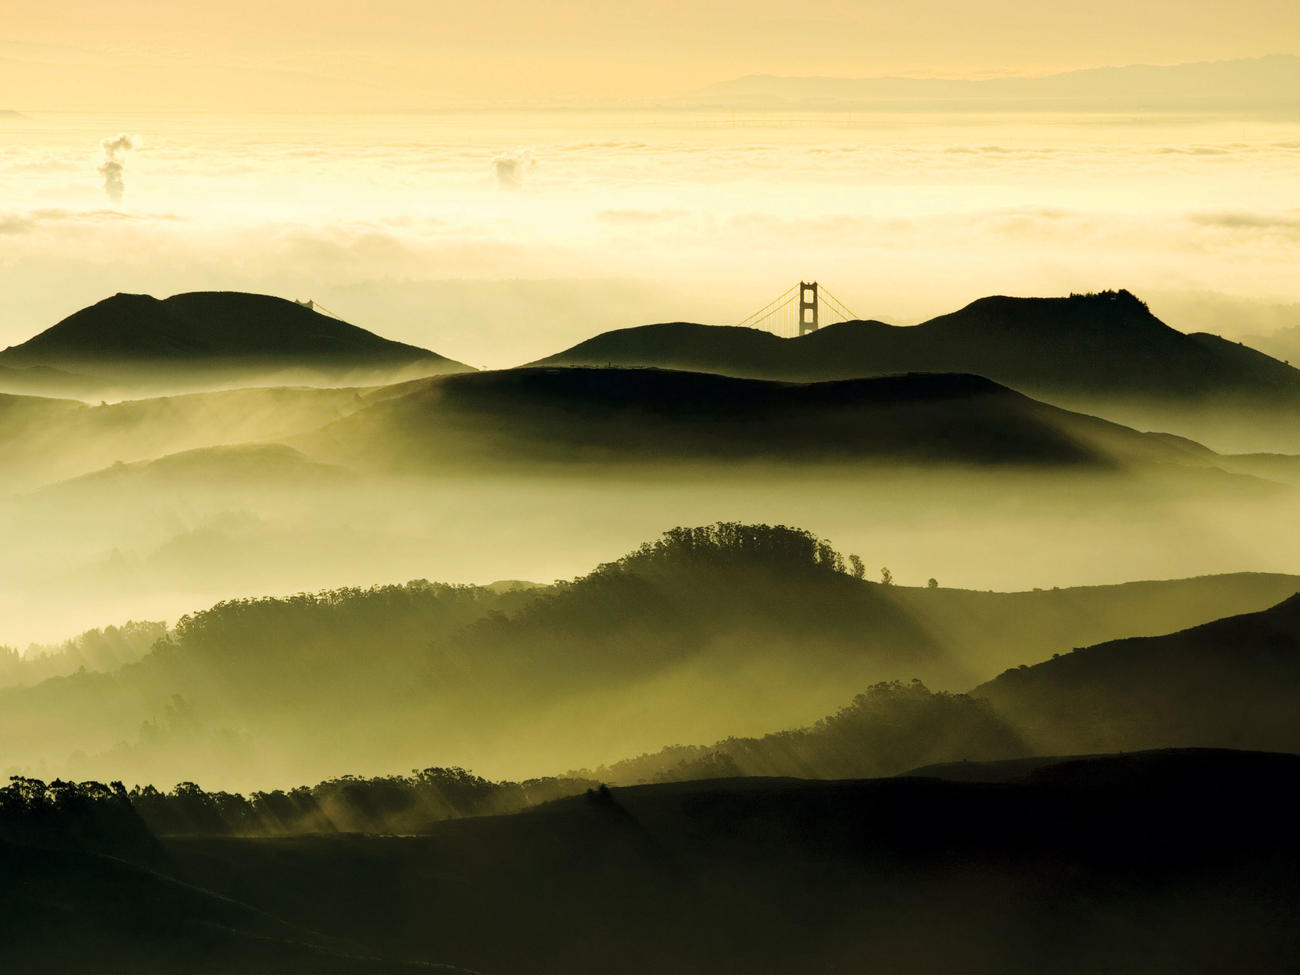
\includegraphics{./images/tam-view.jpeg}

}

\caption{mt. tamalpais}

\end{figure}%

One of our most fundamental goals as data scientists is to produce
predictions that are \emph{good}. In this week's async, we make a
statement of performance that we can use to evaluate how good a job a
predictor is doing, choosing Mean Squared Error.

With the goal of minimizing \(MSE\), then we then present, justify, and
prove that the conditional expectation function (\emph{the CEF}) is the
globally best possible predictor. This is an incredibly powerful result,
and one that serves as the backstop for \textbf{every} other predictor
that you will ever fit, whether that predictor is a ``simple''
regression, or that predictor is a machine learning algorithms (e.g.~a
random forest) or a deep learning algorithm. Read that again:

\begin{quote}
Even the most technologically advanced machine learning algorithms
\emph{cannot possibly} perform better than the conditional expectation
function at making a prediction.
\end{quote}

Why does the CEF do so well? Because it can contain a \emph{vast} amount
of complex information and relationships; in fact, the complexity of the
CEF is a product of the complexity of the underlying probability space.
If that is the case, then why don't we just use the CEF as our predictor
every time?

Well, this is one of the core problems of applied data science work: we
are never given the function that describes the behavior of the random
variable. And so, we're left in a world where we are forced to produce
predictions from simplifications of the CEF. A very strong
simplification, but one that is useful for our puny human brains, is to
restrict ourselves to predictors that make predictions from a linear
combination of input variables.

Why should we make such a strong restriction? After all, the conditional
expectation function might be a fantastically complex combination of
input features, why should we entertain functions that are only linear
combinations? Essentially, this is because we're limited in our ability
to reason about anything more complex than a linear combination.

\section{Thunder Struck}\label{thunder-struck}

\begin{figure}[H]

{\centering 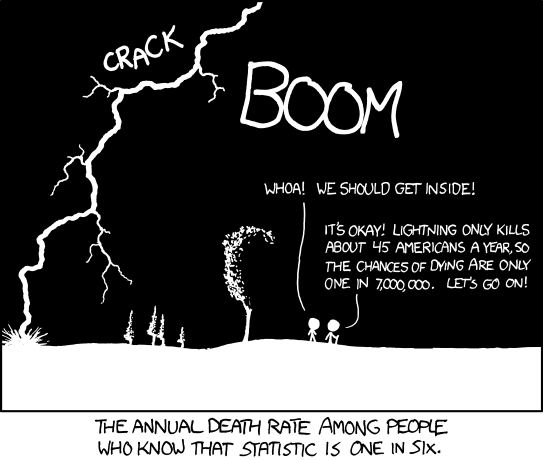
\includegraphics{./images/conditional_risk.png}

}

\caption{thunder struck}

\end{figure}%

\section{Learning Objectives}\label{learning-objectives-3}

At the end of this weeks learning, which includes the asynchronous
lectures, reading the textbook, this live session, and the homework
associated with the concepts, student should be able to

\begin{enumerate}
\def\labelenumi{\arabic{enumi}.}
\tightlist
\item
  \textbf{Recognize} that the conditional expectation function, the
  \emph{CEF}, is a the pure-form, best-possible predictor of a target
  variable given information about other variables.
\item
  \textbf{Recall} that all other predictors, be they linear predictors,
  non-linear predictors, branching predictors, or deep learning
  predictors, are an attempt to approximate the CEF.
\item
  \textbf{Produce} the conditional expectation function as a predictor,
  given joint densities of random variables.
\item
  \textbf{Appreciate} that the best linear predictor, which is a
  restriction of predictors to include only those that are linear
  combinations of variables, can produce reasonable predictions, and
  \textbf{anticipate} that the BLP forms the target of inquiry for
  regression.
\end{enumerate}

\section{Class Announcements}\label{class-announcements-2}

\subsection{Test 1 is releasing to you
today.}\label{test-1-is-releasing-to-you-today.}

The first test is releasing today. There are review sessions scheduled
for this week, practice tests available, and practice problems
available. The format for the test is posted in the course discussion
channel. In addition to your test, your instructor will describe your
responsibilities that are due next week.

\section{Roadmap}\label{roadmap}

\subsection{Rearview Mirror}\label{rearview-mirror}

\begin{itemize}
\tightlist
\item
  Statisticians create a population model to represent the world.
\item
  \(E[X], V[X], Cov[X,Y]\) are ``simple'' summaries of complex joint
  distributions, which are hooks for our analyses.
\item
  They also have useful properties -- for example,
  \(E[X + Y] = E[X] + E[Y]\).
\end{itemize}

\subsection{This week}\label{this-week}

\begin{itemize}
\tightlist
\item
  We look at situations with one or more ``input'' random variables, and
  one ``output.''
\item
  Conditional expectation summarizes the output, given values for the
  inputs.
\item
  The conditional expectation function (CEF) is a predictor -- a
  function that yields a value for the output, give values for the
  inputs.
\item
  The best linear predictor (BLP) summarizes a relationship using a line
  / linear function.
\end{itemize}

\subsection{Coming Attractions}\label{coming-attractions}

\begin{itemize}
\tightlist
\item
  OLS regression is a workhorse of modern statistics, causal analysis,
  etc

  \begin{itemize}
  \tightlist
  \item
    It is also the basis for many other models in classical stats and
    machine learning
  \end{itemize}
\item
  The target that OLS estimates is exactly the BLP, which we're learning
  about this week.
\end{itemize}

\section{Conditional Expectation Function
(CEF),}\label{conditional-expectation-function-cef}

\subsection{Part I}\label{part-i}

Think back to remember the definition of the expectation of \(Y\):

\[
  E[Y] = \int_{-\infty}^\infty y \cdot f_{Y}(y) dy
\]

This week, in the async reading and lectures we added a new concept, the
conditional expectation of \(Y\) given \(X=x \in \text{Supp}[X]\):

\[
  E[Y|X=x] =  \int_{-\infty}^\infty y \cdot f_{Y|X}(y|x) dy
\]

\subsection{Part II}\label{part-ii}

\begin{enumerate}
\def\labelenumi{\arabic{enumi}.}
\tightlist
\item
  What desirable properties of a predictor does the expectation possess
  (note, this is thinking \emph{back} by a week)? What makes these
  properties desirable?
\item
  Turning to the content from this week, how, if at all, does the
  conditional expectation improve on these desirable properties?
\end{enumerate}

\subsection{Part III}\label{part-iii}

\begin{itemize}
\item
  Compare and contrast \(E[Y]\) and \(E[Y|X]\). For example, when you
  look at how these operators are ``shaped'', how are their components
  similar or different?\footnote{Note, when we say ``shaped'' here,
    we're referring to the deeper concept of a statistical functional. A
    statistical functional is a function of a function that maps to a
    real number. So, if \(T\) is the functional that we're thinking of,
    \(\mathcal{F}\) is a family of functions that it might operate on,
    and \(\mathbb{R}\) is the set of real numbers, a statistical
    functional is just \(T: \mathcal{F} \rightarrow \mathbb{R}\). The
    Expectation statistical functional, \(E[X]\) always has the form
    \(\int x f_{X}(x)dx\).)}
\item
  What is \(E[Y|X]\) a function of? What are ``input'' variables to this
  function?
\item
  What, if anything, is \(E[E[Y|X]]\) a function of?
\end{itemize}

\section{Computing the CEF}\label{computing-the-cef}

\begin{itemize}
\tightlist
\item
  Suppose that random variables \(X\) and \(Y\) are jointly continuous,
  with joint density function given by,
\end{itemize}

\[
f(x,y) = 
  \begin{cases}
    2, & 0 \leq x \leq 1, 0 \leq y \leq x \\
    0, & otherwise
\end{cases}
\]

What does the joint PDF of this function look like?

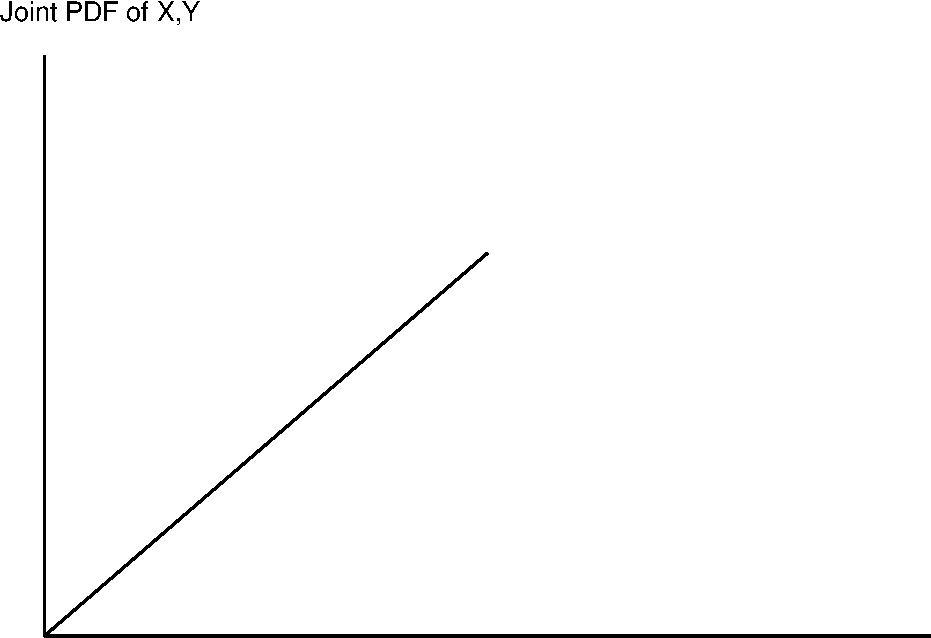
\includegraphics{04-conditional-expectation-and-BLP_files/figure-pdf/create blank plot for pdf-1.pdf}

\subsection{Simple Quantities}\label{simple-quantities}

To begin with, let's compute the simplest quantities:

\begin{itemize}
\tightlist
\item
  What is the expectation of \(X\)?
\item
  What is the expectation of \(Y\)?
\item
  How would you compute the variance of \(X\)? (We're not going to do it
  live).
\end{itemize}

\subsection{Conditional Quantities}\label{conditional-quantities}

\subsubsection{Conditional Expectation}\label{conditional-expectation}

And then, let's think about how to compute the conditional quantities.
To get started, you can use the fact that in week two, we already
computed the conditional probability density function:

\[
f_{Y|X}(y|x) = \begin{cases}
  \frac{1}{x}, & 0 \leq y \leq x \\ 
  0,           & \text{otherwise.}
\end{cases}
\]

With this knowledge on hand, compute the \(CEF[Y|X]\).

\vspace{10cm}

Once you have computed the \(CEF[Y|X]\), use this function to answer the
following questions:

\begin{itemize}
\tightlist
\item
  What is the conditional expectation of \(Y\), given that \(X=x=0\)?
\item
  What is the conditional expectation of \(Y\), given that \(X=x=0.5\)?
\item
  What is the conditional expectation of \(X\), given that \(Y=y=0.5\)?
\end{itemize}

\subsubsection{Conditional Variance}\label{conditional-variance}

\begin{itemize}
\tightlist
\item
  What is the conditional variance function?\footnote{Take a moment to
    strategize just a little bit before you get going on this one. There
    is a way to compute this value that is easier than another way to
    compute this value.}
\end{itemize}

\vspace{20cm}

\begin{itemize}
\tightlist
\item
  Which of the two of these has a lower conditional variances?

  \begin{itemize}
  \tightlist
  \item
    \(V[Y|X=0.25]\); or,
  \item
    \(V[Y|X=0.75]\).
  \end{itemize}
\item
  How does \(V[Y]\) compare to \(V[Y|X=1]\)? Which is larger?
\end{itemize}

\subsection{Conditional Expectation}\label{conditional-expectation-1}

\section{Minimizing the MSE}\label{minimizing-the-mse}

\subsection{Minimizing MSE}\label{minimizing-mse}

Theorem 2.2.20 states,

\begin{quote}
The CEF \(E[Y|X]\) is the ``best'' predictor of \(Y\) given \(X\), where
``best'' means it has the smallest mean squared error (MSE).
\end{quote}

Oh yeah? As a breakout group, \emph{ride shotgun} with us as we prove
that the conditional expectation is the function that produces the
smallest possible Mean Squared Error.

Specifically, \textbf{you group's task} is to justify every transition
from one line to the next using concepts that we have learned in the
course: definitions, theorems, calculus, and algebraic operations.

\subsection{The pudding (aka: ``Where the proof
is'')}\label{the-pudding-aka-where-the-proof-is}

We need to find such function \(g(X): \mathbb{R} \to \mathbb{R}\) that
gives the smallest mean squared error.

First, let MSE be defined as it is in \textbf{Definition 2.1.22}.

\begin{quote}
For a random variable \(X\) and constant \(c \in \mathbb{R}\), the
\emph{mean squared error} of \(X\) about \(c\) is \(E[(x-c)^2]\).
\end{quote}

Second, let us note that since \(g(X)\) is just a function that maps
onto \(\mathbb{R}\), that for some particular value of \(X=x\), \(g(X)\)
maps onto a constant value.

\begin{itemize}
\tightlist
\item
  Deriving a Function to Minimize MSE
\end{itemize}

\[
\begin{aligned}
  E[(Y - g(X))^2|X]
      &= E[Y^2 - 2Yg(X) + g^2(X)|X]                                \\
      &= E[Y^2|X] + E[-2Yg(X)|X] + E[g^2(X)|X]                     \\
      &= E[Y^2|X] - 2g(X)E[Y|X] + g^2(X)E[1|X]                     \\
      &= (E[Y^2|X] - E^2[Y|X]) + (E^2[Y|X] - 2g(X)E[Y|X] + g^2(X)) \\
      &= V[Y|X] + (E^2[Y|X] - 2g(X)E[Y|X] + g^2(X))                \\
      &= V[Y|X] + (E[Y|X] - g(X))^2                                \\
\end{aligned} 
\]

Notice too that we can use the \emph{Law of Iterated Expectations} to do
something useful. (This is a good point to talk about how this theorem
works in your breakout groups.)

\[
\begin{aligned}
  E[(Y-g(X))^2] &= E\big[E[(Y-g(X))^2|X]\big]     \\ 
    &=E\big[V[Y|X]+(E[Y|X]-g(X))^2\big]           \\
    &=E\big[V[Y|X]\big]+E\big[(E[Y|X]-g(X))^2\big]\\
\end{aligned}
\]

\begin{itemize}
\tightlist
\item
  \(E[V[Y|X]]\) doesn't depend on \(g\); and,
\item
  \(E[(E[Y|X]-g(X))^2] \geq 0\).
\end{itemize}

\(\therefore g(X) = E[Y|X]\) gives the smallest \(E[(Y-g(X))^2]\)

\subsection{The Implication}\label{the-implication}

If you are choosing some \(g\), you can't do better than
\(g(x) = E[Y|X=x]\).

\section{Working with the BLP}\label{working-with-the-blp}

Why Linear?

\begin{itemize}
\tightlist
\item
  In some cases, we might try to estimate the CEF. More commonly,
  however, we work with linear predictors. Why?
\end{itemize}

\begin{itemize}
\tightlist
\item
  We don't know joint density function of \(Y\). So, it is ``difficult''
  to derive a suitable CEF.
\item
  To estimate \emph{flexible} functions requires considerably more data.
  Assumptions about distribution (e.g.~a linear form) allow you to
  leverage those assumptions to learn `more' from the same amount of
  data.
\item
  Other times, the CEF, even if we \emph{could} produce an estimate,
  might be so complex that it isn't useful or would be difficult to work
  with.
\item
  And, many times, linear predictors (which might seem trivially simple)
  actually do a very good job of producing predictions that are `close'
  or useful.
\end{itemize}

\section{Joint Distribution Practice}\label{joint-distribution-practice}

\subsection{Professorial Mistakes (Discrete
RVs)}\label{professorial-mistakes-discrete-rvs}

\begin{itemize}
\item
  Let the number of questions that students ask be a RV, \(X\).\\
\item
  Let \(X\) take on values: \(\{1, 2, 3\}\), each with probability
  \(1/3\).\\
\item
  Every time a student asks a question, the instructor answers
  incorrectly with probability \(1/4\), independently of other
  questions.
\item
  Let the RV \(Y\) be number of incorrect responses.
\item
  \textbf{Questions:}

  \begin{itemize}
  \tightlist
  \item
    Compute the expectation of \(Y\), conditional on \(X\), \(E[Y|X]\)
  \item
    Using the law of iterated expectations, compute
    \(E[Y] = E\big[E[Y|X]\big]\).
  \end{itemize}
\end{itemize}

\subsection{Continuous BLP}\label{continuous-blp}

\begin{itemize}
\tightlist
\item
  Recall the PDF that we worked with earlier to produce the
  \$CEF{[}Y\textbar X{]}.
\end{itemize}

\[
f(x,y) = 
  \begin{cases}
    2, & 0 \leq x \leq 1, 0 \leq y \leq x \\
    0, & otherwise
\end{cases}
\]

Find the \(BLP\) for \(Y\) as a function of \(X\). What, if anything, do
you notice about this \(BLP\) and the \(CEF\)?

\vspace{20cm}

\part{Sampling and Testing}

In this section we will introduce the basics of sampling and testing.

\chapter{Learning from Random
Samples}\label{learning-from-random-samples}

\begin{figure}[H]

{\centering \includegraphics{./images/south_hall.jpeg}

}

\caption{south hall}

\end{figure}%

This week, we're coming into the big turn in the class, from probability
theory to sampling theory.

In the probability theory section of the course, we developed the
\emph{theoretically} \textbf{best} possible set of models. Namely, we
said that if our goal is to produce a model that minimizes the Mean
Squared Error that \emph{expectation} and \emph{conditional expectation}
are as good as it gets. That is, if we only have the outcome series,
\(Y\), we cannot possibly improve upon \(E[Y]\), the expectation of the
random variable \(Y\). If we have additional data on hand, say \(X\) and
\(Y\), then the best model of \(Y\) given \(X\) is the conditional
expectation, \(E[Y|X]\).

We have also said that because this conditional expectation function
might be complex, and hard to inform with data, that we might also be
interested in a principled simplification of the conditional expectation
function -- the simplification that requires our model be a line.

With this simplification in mind, we derived the linear system that
produces the minimum MSE: the ratio of covariance between variables to
variance of the predictor:

\[
  \beta_{BLP} = \frac{Cov[Y,X]}{V[X]}. 
\]

We noted, quickly, that the simple case of only two variables -- an
outcome and a single predictor -- generalizes nicely into the
(potentially very) many dimensional case. If the many-dimensional
\(BLP\) is denoted as
\(g(\mathbf{X}) = b_{0} + b_{1}X_{1} + \dots + b_{k}X_{k}\), then we can
arrive at the sloped between one particular predictor, \(X_{k}\), and
the outcome, \(Y\), as:

\[
  b_{k} = \frac{\partial g(\mathbf{X})}{\partial X_{k}}. 
\]

\section{Goals, Framework, and Learning
Objectives}\label{goals-framework-and-learning-objectives}

\subsection{Class Announcements}\label{class-announcements-3}

\begin{itemize}
\tightlist
\item
  You're done with probability theory. \textbf{Yay!}
\item
  You're also done with your first test. \textbf{Double Yay!}
\item
  We're going to have a second test in a few weeks. Then we're done
  testing for the semester \textbf{Yay?}
\end{itemize}

\subsection{Learning Objectives}\label{learning-objectives-4}

At the end of this week, students will be able to

\begin{enumerate}
\def\labelenumi{\arabic{enumi}.}
\tightlist
\item
  \textbf{Understand} what iid sampling is, and evaluate whether the
  assumption of iid sampling is sufficiently plausible to engage in
  frequentist modeling.
\item
  \textbf{Appreciate} that with iid sampling, summarizing functions of
  random variables are, themselves, random variables with probability
  distributions and values that they obtain.
\item
  \textbf{Recall} the definition of an estimator,
\item
  \textbf{Recall} definition of an estimator, \textbf{state} and
  \textbf{understand} the desirable properties of estimators, and
  \textbf{evaluate} whether an estimator possesses those desirable
  properties.
\item
  \textbf{Distinguish} between the concepts of \{expectation \& sample
  mean\}, \{variance \& unbiased sample variance estimator,
  sampling-based variance in the sample mean\}.
\end{enumerate}

\subsection{Roadmap}\label{roadmap-1}

\subsubsection{Where We're Going -- Coming
Attractions}\label{where-were-going-coming-attractions}

\begin{itemize}
\tightlist
\item
  We're going to start bringing data into our work
\item
  First, we're going to develop a testing framework that is built on
  sampling theory and reference distributions: these are the
  \textbf{frequentist tests}.
\item
  Second, we're going to show that OLS regression is the sample
  estimator of the BLP. This means that OLS regression produces
  estimates of the BLP that have known convergence properties.
\item
  Third, we're going combine the frequentist testing framework with OLS
  estimation to produce a full regression testing framework.
\end{itemize}

\subsubsection{Where We've Been -- Random Variables and Probability
Theory}\label{where-weve-been-random-variables-and-probability-theory}

Statisticians create a model (also known as the population model) to
represent the world. This model exists as joint probability densities
that govern the probabilities that any series of events occurs at the
same time. This joint probability of outcomes can be summarized and
described with lower-dimensional summaries like the expectation,
variance, covariance. While the expectation is a summary that contains
information on about one marginal distribution (i.e.~the outcome we are
interested in) we can produce predictive models that update, or
\emph{condition} the expectation based on other random variables. This
summary, the \textbf{conditional expectation} is the best possible
(measured in terms of minimizing mean squared error) predictor of an
outcome. We might simplify this conditional expectation predictor in
many ways; the most common is to simplify to the point that the
predictor is constrained to be a line or plane. This is known as the
Best Linear Predictor.

\subsubsection{Where we Are}\label{where-we-are}

\begin{itemize}
\tightlist
\item
  We want to fit models -- use data to set their parameter values.
\item
  A sample is a set of random variables
\item
  Sample statistics are functions of a sample, and they are random
  variables
\item
  Under iid and other assumptions, we get useful properties:

  \begin{itemize}
  \tightlist
  \item
    Statistics may be consistent estimators for population parameters
  \item
    The distribution of sample statistics may be asymptotically normal
  \end{itemize}
\end{itemize}

\section{Key Terms and Assumptions}\label{key-terms-and-assumptions}

\subsection{IID}\label{iid}

We use an abbreviation for the sampling process that under girds our
frequentist statistics. That abbreviation, \textbf{IID}, while short,
contains two powerful requirements of our data sampling process.

IID sampling is:

\begin{enumerate}
\def\labelenumi{\arabic{enumi}.}
\tightlist
\item
  \textbf{Independent}. The first \textbf{I} in the abbreviation, this
  independence requirement is similar to the independence concept that
  we've used in the probability theory section of the course. When
  samples are independent, the result of any one sample is not
  informative about the value of any of the other samples.
\item
  \textbf{Identically Distributed}. The \textbf{ID} in the abbreviation,
  this requirement means that all samples are drawn from the same
  distribution.
\end{enumerate}

It might be tempting to imagine that IID samples are just \emph{``random
samples''}, but it is worth noting that IID sampling has the two
specific requirements noted above, and that these requirements are more
stringent than a ``randomness'' criteria.

When we are thinking about IID samples, and evaluating whether the
sample do, in point of fact, meet both of the requirements, it is
\emph{crucial} to make an explicit statement about the reference
population that is under consideration.

For example, suppose that you were interested in learning about
life-satisfaction and your reference population are the peoples who live
in the United States. Further, suppose that you decide to produce an
estimate of this using a sample drawn from UC Berkeley undergraduate
students during
\href{https://teaching.berkeley.edu/sites/default/files/rrr_guidelines.pdf}{RRR
week}? There are several flaws in this design:

\begin{enumerate}
\def\labelenumi{\arabic{enumi}.}
\tightlist
\item
  There is a key \textbf{research design} issue: a sample drawn from
  Berkeley undergraduates is going to be \emph{essentially}
  uninformative of a US resident reference population!
\item
  There is a key \textbf{statistical} issue: the population of Berkeley
  undergraduates are not really an independent sample from the entire US
  resident reference population. Once you learn the age of someone from
  the Berkeley student population, you can make an conditional guess
  about the age of the next sample that will be closer than was possible
  before the first sample. The same goes for life-satisfaction: When you
  learn about the life-satisfaction from the first undergrad (who is
  miserable because they have their Stat 140 final coming up) while they
  are studying for their finals) you can make a conditionally better
  guess about the satisfaction of the next undergrad.
\end{enumerate}

Notice that these violations of the IID requirements only arise because
our reference population is the US resident population. If, instead, the
reference population were ``Berkeley undergrads'' then the sampling
process \emph{would} satisfy the requirements of an IID process.

\begin{itemize}
\tightlist
\item
  How, or why, can a change in the reference population make an
  identical sampling process move from one that we can consider IID to
  one that we cannot consider IID?
\end{itemize}

\subsubsection{It this IID?}\label{it-this-iid}

For each of the following scenarios, is the IID assumption plausible?

\begin{enumerate}
\def\labelenumi{\arabic{enumi}.}
\tightlist
\item
  Call a random phone number. If someone answers, interview all persons
  in the household. Repeat until you have data on 100 people.
\item
  Call a random phone number, interview the person if they are over 30.
  Repeat until you have data on 100 people.
\item
  Record year-to-date price change for 20 largest car manufacturers.
\item
  Measure net exports per GDP for all 195 countries recognized by the
  UN.
\end{enumerate}

\section{Estimators}\label{estimators}

In our presentation of this week's materials, we choose to switch the
presentation of statistics and estimators, electing to discuss
properties that we would like estimators to posses, before we actually
introduce any specific estimators.

\subsection{Three properties of
estimators}\label{three-properties-of-estimators}

What are the three desirable properties of estimators?

\begin{enumerate}
\def\labelenumi{\arabic{enumi}.}
\tightlist
\item
\item
\item
\end{enumerate}

Is one these properties \emph{more} important than another? If you had
to force-rank these properties in terms of their importance, which is
the most, and which the least important? Why?

\section{Estimator Property: Biased or
Unbiased?}\label{estimator-property-biased-or-unbiased}

\begin{enumerate}
\def\labelenumi{\arabic{enumi}.}
\tightlist
\item
  First, for a general case: Suppose that you have chosen some
  particular estimator, \(\hat{\theta}\) to estimate some
  characteristic, \(\theta\) of a random variable. How do you know if
  this estimator is unbiased?
\item
  Second, for a specific case: Define the ``sample average'' to be the
  following: \(\frac{1}{n}\sum_{i=1}^{N} x_{i}\). Prove that this sample
  average estimator is an unbiased estimator of \(E[X]\).
\item
  Third (easier), for a different specific case: Define the ``smample
  smaverage'' to be the following \(\frac{1}{n^2}\sum_{i=1}^{N} x_{i}\).
  Prove that the smample smaverage is a biased estimator of \(E[X]\).
\item
  Fourth (harder): Define the geometric mean to be
  \[\left(\prod_{i=1}^{N}x_{i}\right)^{\frac{1}{N}}\]. Prove that the
  geometric mean is a biased estimator of \(E[X]\).
\end{enumerate}

\subsection{Is it unbiased, with data?}\label{is-it-unbiased-with-data}

Suppose that you're getting data from the following process:

\begin{Shaded}
\begin{Highlighting}[]
\NormalTok{random\_distribution }\OtherTok{\textless{}{-}} \ControlFlowTok{function}\NormalTok{(number\_samples) \{ }
  
\NormalTok{  d1 }\OtherTok{\textless{}{-}} \FunctionTok{c}\NormalTok{(}\FloatTok{1.0}\NormalTok{, }\FloatTok{2.0}\NormalTok{)}
\NormalTok{  d2 }\OtherTok{\textless{}{-}} \FunctionTok{c}\NormalTok{(}\FloatTok{1.1}\NormalTok{, }\FloatTok{2.1}\NormalTok{)}
\NormalTok{  d3 }\OtherTok{\textless{}{-}} \FunctionTok{c}\NormalTok{(}\FloatTok{1.5}\NormalTok{, }\FloatTok{2.5}\NormalTok{)}

\NormalTok{  distribution\_chooser }\OtherTok{=} \FunctionTok{sample}\NormalTok{(}\AttributeTok{x=}\DecValTok{1}\SpecialCharTok{:}\DecValTok{3}\NormalTok{, }\AttributeTok{size=}\DecValTok{1}\NormalTok{)}
  
  \ControlFlowTok{if}\NormalTok{(distribution\_chooser }\SpecialCharTok{==} \DecValTok{1}\NormalTok{) \{ }
\NormalTok{    x\_ }\OtherTok{\textless{}{-}} \FunctionTok{runif}\NormalTok{(}\AttributeTok{n=}\NormalTok{number\_samples, }\AttributeTok{min=}\NormalTok{d1[}\DecValTok{1}\NormalTok{], }\AttributeTok{max=}\NormalTok{d1[}\DecValTok{2}\NormalTok{])  }
\NormalTok{  \} }\ControlFlowTok{else} \ControlFlowTok{if}\NormalTok{(distribution\_chooser }\SpecialCharTok{==} \DecValTok{2}\NormalTok{) \{ }
\NormalTok{    x\_ }\OtherTok{\textless{}{-}} \FunctionTok{runif}\NormalTok{(}\AttributeTok{n=}\NormalTok{number\_samples, }\AttributeTok{min=}\NormalTok{d2[}\DecValTok{1}\NormalTok{], }\AttributeTok{max=}\NormalTok{d2[}\DecValTok{2}\NormalTok{]) }
\NormalTok{  \} }\ControlFlowTok{else} \ControlFlowTok{if}\NormalTok{(distribution\_chooser }\SpecialCharTok{==} \DecValTok{3}\NormalTok{) \{ }
\NormalTok{    x\_ }\OtherTok{\textless{}{-}} \FunctionTok{runif}\NormalTok{(}\AttributeTok{n=}\NormalTok{number\_samples, }\AttributeTok{min=}\NormalTok{d3[}\DecValTok{1}\NormalTok{], }\AttributeTok{max=}\NormalTok{d3[}\DecValTok{2}\NormalTok{])}
\NormalTok{  \}}
  \FunctionTok{return}\NormalTok{(x\_)}
\NormalTok{\}}

\FunctionTok{random\_distribution}\NormalTok{(}\AttributeTok{number\_samples=}\DecValTok{10}\NormalTok{)}
\end{Highlighting}
\end{Shaded}

\begin{verbatim}
 [1] 1.599740 1.836487 1.847496 1.657702 1.247919 1.473912 1.818252 1.199693
 [9] 1.870626 1.924699
\end{verbatim}

\begin{Shaded}
\begin{Highlighting}[]
\FunctionTok{mean}\NormalTok{(}\FunctionTok{random\_distribution}\NormalTok{(}\AttributeTok{number\_samples=}\DecValTok{10000}\NormalTok{))}
\end{Highlighting}
\end{Shaded}

\begin{verbatim}
[1] 1.496155
\end{verbatim}

Notice that, there are two forms of inherent uncertainty in this
function:

\begin{enumerate}
\def\labelenumi{\arabic{enumi}.}
\tightlist
\item
  There is uncertainty about the distribution that we are getting draws
  from; and,
\item
  Within a distribution, we're getting draws at random from a population
  distribution.
\end{enumerate}

This class of function, the \texttt{r*} functions, are the
implementation of random generative processes within the R language.
Look into \texttt{?distributions} as a class to see more about this
process.

Suppose that you chose to use the same sample average estimator as a
means of producing an estimate of the population expected value,
\(E[X]\). Suppose that you get the following draws:

\begin{Shaded}
\begin{Highlighting}[]
\NormalTok{draws }\OtherTok{\textless{}{-}} \FunctionTok{random\_distribution}\NormalTok{(}\AttributeTok{number\_samples=}\DecValTok{10}\NormalTok{)}
\NormalTok{draws}
\end{Highlighting}
\end{Shaded}

\begin{verbatim}
 [1] 1.698962 1.546228 2.106683 1.580572 2.381539 1.608441 2.145225 1.521661
 [9] 1.866070 1.534782
\end{verbatim}

\begin{Shaded}
\begin{Highlighting}[]
\FunctionTok{mean}\NormalTok{(draws)}
\end{Highlighting}
\end{Shaded}

\begin{verbatim}
[1] 1.799016
\end{verbatim}

Is this sample average an unbiased estimator for the population expected
value? How do you know?

\section{Estimator Property:
Consistency}\label{estimator-property-consistency}

\emph{Foundations} makes another of their jokes when they write, on page
105,

\begin{quote}
``Consistency is a simple notion: if we had enough data, the probability
that our estimate \(\hat{\theta}\) would be far from the truth,
\(\theta\), would be small.''
\end{quote}

\textbf{How do we determine if a particular estimator, \(\hat{\theta}\)
is a consistent estimator for our parameter of interest?}

There are at least two ways:

\begin{enumerate}
\def\labelenumi{\arabic{enumi}.}
\tightlist
\item
  The estimator is unbiased, and has a sampling variance that decreases
  as we add data; or,
\item
  We can use Chebyshev's to place a bound on the estimator, showing that
  as we add data, the estimator converges in probability to \(\theta\).
\end{enumerate}

The first notion of convergence requires an understanding of sampling
variance:

The sampling variance of an estimator is a statement about how much
dispersion due to random sampling, is present in the estimator. We
defined the variance of a random variable to be
\(E\left[(X - E[X])^{2}\right]\), The sampling variance uses this same
definition, but we work with it slightly differently when we are
considering sampling variance.

In particular, when we are considering sampling variance, we do not
typically got as far as actually computing the variance of the
underlying random variable? \emph{Why?} Because, if we're working in a
sampling scenario, it is unlikely that we have access to the underlying
function that governs the PDF of the random variable.

Instead, we typically start from a statement of the estimator that is
under consideration, and apply the variance operator against that
estimator. Consider, for example, forming a statement about the sampling
variance of the sample average.

Let \(\overline{X} \equiv\) ``sample average''
\(\equiv \frac{1}{n}\sum_{i=1}^{n}X_{i}\) be the normal form of the
sample average.

Earlier, we proved that \(\overline{X}\) is an unbiased estimator of
\(E[X]\).

What is the sampling variance of the sample average?

\vspace{20cm}

Using the statement that you have just produced, would you say that the
sample average is a consistent estimator for the population expectation
of a random variable?

\section{Understanding Sampling
Distributions}\label{understanding-sampling-distributions}

How do sampling distributions change as we add data to them? This is
going to both motivate convergence, and also play forward into the
Central Limit Theorem. Let's work through an example that begins with a
case that we can think through and draw ourselves. Once we feel pretty
good about the \emph{very} small sample, then we will rely on R to do
the work when we expand the example beyond what we can draw ourselves.

Suppose that \(X\) is a Bernoulli random variable representing an unfair
coin. Suppose that the coin has a 70\% chance of coming up heads:
\(P(X=1) = 0.7\).

\begin{itemize}
\tightlist
\item
  To begin, suppose that you take that coin, and you toss it two times:
  you have an iid sample of size 2, \((X_1,X_2)\).
\item
  \emph{What is the sampling distribution of the sample average, of this
  sample of size two?}
\item
  On the axes below, draw the probability distribution of
  \(\overline X = \frac{X_1+X_2}{2}\).
\end{itemize}

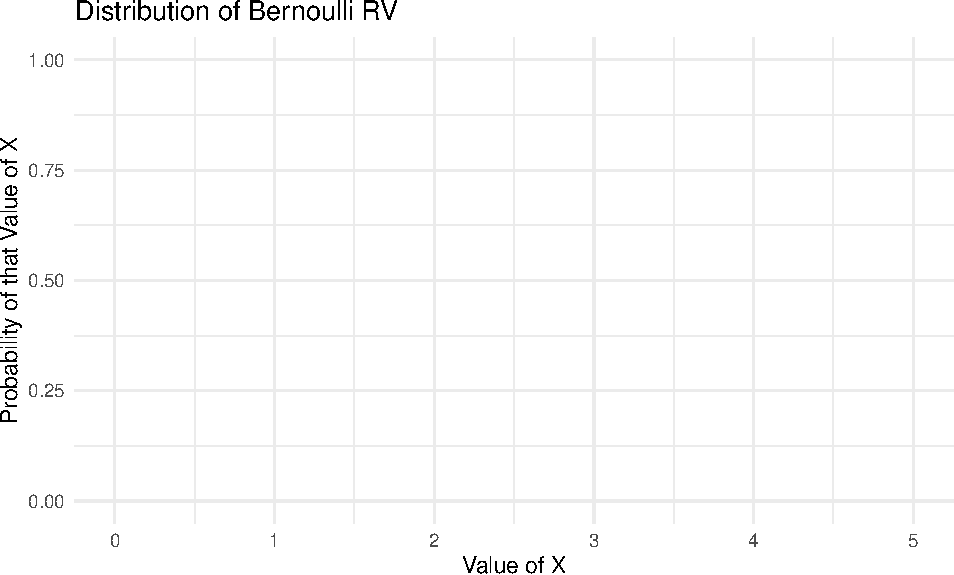
\includegraphics{05-sampling-theory_files/figure-pdf/make axes-1.pdf}

\begin{itemize}
\tightlist
\item
  What if you took four samples? What would the sampling distribution of
  \(\overline{X}\) look like? \emph{Draw this onto the axis above.}
\item
  Explain the difference between a population distribution and the
  sampling distribution of a statistic.
\item
  Why do we want to know things about the sampling distribution of a
  statistic?
\end{itemize}

We are going to write a function that, essentially, just wraps a
built-in function with a new name and new function arguments. This is,
generally, bad coding practice -- because it is changing the default
lexicon than a collaborator needs to be aware of -- but it is useful for
teaching purposes here.

\begin{itemize}
\tightlist
\item
  The \texttt{number\_of\_simulations} argument to the
  \texttt{toss\_coin} function basically just adjusts the precision of
  our simulation study.
\item
  Let's set, and keep this at \(1000\) simulations. But, if you're
  curious, you could set this to be \(5\), or \(10\) and evaluate what
  happens.
\end{itemize}

\begin{Shaded}
\begin{Highlighting}[]
\NormalTok{toss\_coin }\OtherTok{\textless{}{-}} \ControlFlowTok{function}\NormalTok{(}
    \AttributeTok{number\_of\_simulations=}\DecValTok{1000}\NormalTok{, }
    \AttributeTok{number\_of\_tosses=}\DecValTok{2}\NormalTok{, }
    \AttributeTok{prob\_heads=}\FloatTok{0.7}\NormalTok{) \{ }
  
  \DocumentationTok{\#\# number of simulations is just how many times we want to re{-}run the experiment}
  \DocumentationTok{\#\# number of tosses is the number of coins we\textquotesingle{}re going to toss.}
\NormalTok{  number\_of\_heads }\OtherTok{\textless{}{-}} \FunctionTok{rbinom}\NormalTok{(}\AttributeTok{n=}\NormalTok{number\_of\_simulations, }\AttributeTok{size=}\NormalTok{number\_of\_tosses, }\AttributeTok{prob=}\NormalTok{prob\_heads)}
\NormalTok{  sample\_average  }\OtherTok{\textless{}{-}}\NormalTok{ number\_of\_heads }\SpecialCharTok{/}\NormalTok{ number\_of\_tosses}
  \FunctionTok{return}\NormalTok{(sample\_average)}
\NormalTok{\}}

\FunctionTok{toss\_coin}\NormalTok{(}\AttributeTok{number\_of\_simulations=}\DecValTok{10}\NormalTok{, }\AttributeTok{number\_of\_tosses=}\DecValTok{2}\NormalTok{, }\AttributeTok{prob\_heads=}\FloatTok{0.7}\NormalTok{)}
\end{Highlighting}
\end{Shaded}

\begin{verbatim}
 [1] 0.5 0.0 1.0 1.0 0.0 1.0 1.0 1.0 1.0 1.0
\end{verbatim}

\begin{Shaded}
\begin{Highlighting}[]
\NormalTok{ncoins }\OtherTok{\textless{}{-}} \DecValTok{10}

\NormalTok{coin\_result\_005 }\OtherTok{\textless{}{-}} \FunctionTok{toss\_coin}\NormalTok{(}
  \AttributeTok{number\_of\_simulations =} \DecValTok{10000}\NormalTok{,}
  \AttributeTok{number\_of\_tosses =}\NormalTok{ ncoins, }
  \AttributeTok{prob\_heads =} \FloatTok{0.005}
\NormalTok{  )}

\NormalTok{coin\_result\_05 }\OtherTok{\textless{}{-}} \FunctionTok{toss\_coin}\NormalTok{(}
  \AttributeTok{number\_of\_simulations =} \DecValTok{10000}\NormalTok{,}
  \AttributeTok{number\_of\_tosses =}\NormalTok{ ncoins, }
  \AttributeTok{prob\_heads =} \FloatTok{0.5}
\NormalTok{  )}

\NormalTok{plot\_005 }\OtherTok{\textless{}{-}} \FunctionTok{ggplot}\NormalTok{() }\SpecialCharTok{+} 
    \FunctionTok{aes}\NormalTok{(}\AttributeTok{x=}\NormalTok{coin\_result\_005) }\SpecialCharTok{+} 
    \FunctionTok{geom\_histogram}\NormalTok{(}\AttributeTok{bins=}\DecValTok{50}\NormalTok{) }\SpecialCharTok{+} 
    \FunctionTok{geom\_vline}\NormalTok{(}\AttributeTok{xintercept=}\FloatTok{0.005}\NormalTok{, }\AttributeTok{color=}\StringTok{\textquotesingle{}\#003262\textquotesingle{}}\NormalTok{, }\AttributeTok{linewidth=}\DecValTok{2}\NormalTok{)}

\NormalTok{plot\_05 }\OtherTok{\textless{}{-}} \FunctionTok{ggplot}\NormalTok{() }\SpecialCharTok{+} 
    \FunctionTok{aes}\NormalTok{(}\AttributeTok{x=}\NormalTok{coin\_result\_05) }\SpecialCharTok{+} 
    \FunctionTok{geom\_histogram}\NormalTok{(}\AttributeTok{bins=}\DecValTok{50}\NormalTok{) }\SpecialCharTok{+} 
    \FunctionTok{geom\_vline}\NormalTok{(}\AttributeTok{xintercept=}\FloatTok{0.5}\NormalTok{, }\AttributeTok{color=}\StringTok{\textquotesingle{}\#003262\textquotesingle{}}\NormalTok{, }\AttributeTok{linewidth=}\DecValTok{2}\NormalTok{)}

\NormalTok{plot\_005 }\SpecialCharTok{/} 
\NormalTok{  plot\_05}
\end{Highlighting}
\end{Shaded}

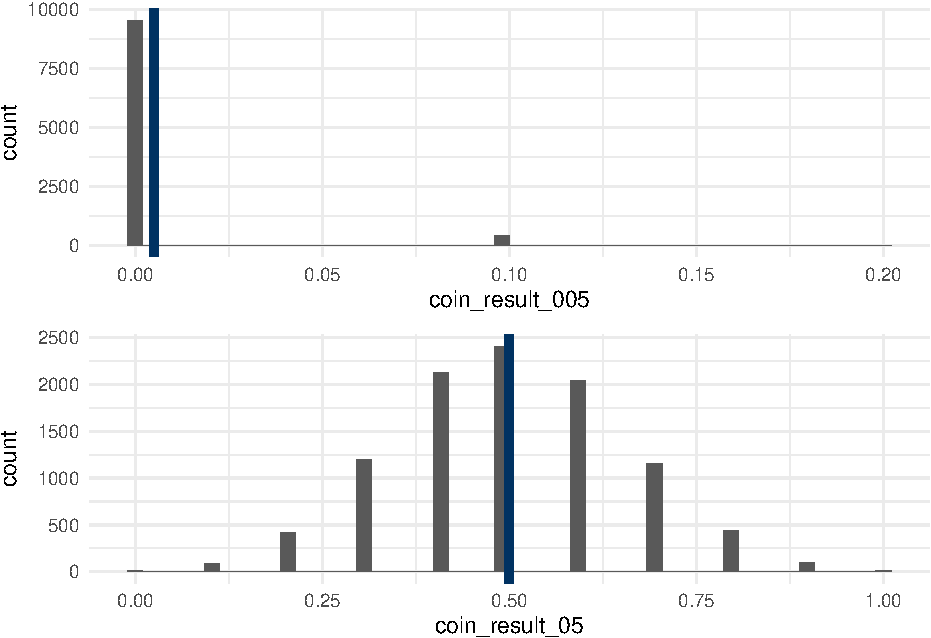
\includegraphics{05-sampling-theory_files/figure-pdf/toss coins and plot-1.pdf}

In the plot that you have drawn above, pick some value, \(\epsilon\)
that is the distance away from the true expected value of this
distribution.

\begin{itemize}
\tightlist
\item
  What proportion of the sampling distribution is further away than
  \(E[X] \pm \epsilon\)?
\item
  When we toss the coin only two times, we can quickly draw out the
  distribution of \(\overline{X}\), and can form a statement about the
  \(P(E[X] - \epsilon \leq  \overline{X} \leq E[X] + \epsilon)\).
\item
  What if we toss the coin ten times? We can still use the IID nature of
  the coin to figure out the \emph{true}
  \(P(\overline{X} = 0), P(\overline{X} = 1), \dots, P(\overline{X} = 10)\),
  but it is going to start to take some time. This is where we rely on
  the simulation to start speeding up our learning.
\item
  As we toss more and more coins,
  \(\overline X_{(100)} \rightarrow \overline X_{(10000)}\) what will
  the value of \(\overline X\) get closer to? What law generates this,
  and why does this law generate this result?
\end{itemize}

\section{Write Code to Demo the Central Limit Theorem
(CLT)}\label{write-code-to-demo-the-central-limit-theorem-clt}

When you were reading for this week, did you sense the palpable
\emph{joy} of the authors when they were writing about the central limit
theorem?

\begin{quote}
We now preset what is often considered the most profound and important
theorem in statistics.
\end{quote}

Wow. What excitement.

On its own, the result that \emph{across a broad range of generative
functions the distribution of sample averages converges in distribution
to follow a normal distribution} would be a statistical curiosity. Along
the lines of ``did you know that dinosaurs might have had feathers,''
or, ``avocado trees reproduce using 'protogynous dichogamy''. While
these factoids might be useful on your quiz-bowl team, they don't get us
very far down the line as practicing data scientists.

However, there is a \textbf{very} useful consequence of this convergence
in distribution that we will explore in detail over the coming two
weeks: because \emph{so many} distributions produce sample averages that
converge in distribution to a normal distribution, we can put together a
testing framework for sample averages that works for an \emph{agnostic}
set of random variables. Wait for that next week, but know that there's
a reason that we're as excited about this statement as we are.

\subsection{Part 1}\label{part-1}

To begin with, we will use fair coins that have an equal probability
landing heads and tails.

\begin{enumerate}
\def\labelenumi{\arabic{enumi}.}
\tightlist
\item
  Modify the function argument below so that it conduct \textbf{one}
  simulations, and in each simulation tosses \textbf{ten} coins, each
  with an \textbf{equal} probability of landing heads and tails. Look
  into the \texttt{toss\_coin} function: is there a point that this
  function is producing a sample average? If so, where?
\item
  Save values from the \texttt{toss\_coin} function into an object,
  called \texttt{sample\_mean}.
\end{enumerate}

\begin{Shaded}
\begin{Highlighting}[]
\CommentTok{\# toss\_coin()}
\end{Highlighting}
\end{Shaded}

The sample mean is a random variable -- it is a function that maps from
a random generative process' sample space (the number of heads shown on
dice) to the real numbers. To try to make this clear, visualize a larger
number of simulations on the \texttt{toss\_coin} function. That is,
increase the \texttt{number\_of\_simulations} to be 10, or 100. and plot
a histogram of the results. This is quite similar to what we have done
earlier.

\begin{Shaded}
\begin{Highlighting}[]
\CommentTok{\# toss\_coin()}
\end{Highlighting}
\end{Shaded}

If you replicate the simulation with \textbf{ten} coins enough times,
will the distribution ever look normal? Why or why not?

\subsection{Part 2}\label{part-2}

For this part, we'll continue to study a fair coin.

What happens if you change the number of coins that you're tossing?
Here, set \texttt{number\_of\_simulations=1000}, and examine what
happens if you alter the number of coins that you're tossing? Is there a
point where this distribution starts to ``look normal'' to you? (Later
in the semester, we'll formalize a test for this ``looks normal''
concept).

\subsection{Part 3}\label{part-3}

What would happen if the coin was very, very unfair? For this part,
study a coin that has a \texttt{prob\_heads=0.01}. This is an example of
a highly skewed random variable.

Start your study here tossing three coins, \texttt{number\_of\_coins=3}.
What does this distribution look like?

What happens as you increase the number of coins that you're tossing? Is
there a point that the distribution starts to look normal?

\subsection{Discussion Questions About the
CLT}\label{discussion-questions-about-the-clt}

\begin{enumerate}
\def\labelenumi{\arabic{enumi}.}
\tightlist
\item
  How does the skewness of the population distribution affect the
  applicability of the Central Limit Theorem? What lesson can you take
  for your practice of statistics?
\item
  Name a variable you would be interested in measuring that has a
  substantially skewed distribution.
\item
  One definition of a heavy tailed distribution is one with infinite
  variance. For example, you can use the \texttt{rcauchy} command in R
  to take draws from a Cauchy distribution, which has heavy tails. Do
  you think a ``heavy tails'' distribution will follow the CLT? What
  leads you to this intuition?
\end{enumerate}

\section{Errors with Standard Errors}\label{errors-with-standard-errors}

Talking about variance and sampling variance is hard, because the terms
sound \textbf{very} similar, but have important distinctions in what
they mean. For example, the ``variance'' is not the same as the
``unbiased sample variance'' which is also not the same as the
``sampling variance of the sample average''. :sob:

Standard errors are a statement about the sampling variance of the
sample average. But, related to this concept are the ideas of the
\emph{Population Variance}, the \emph{Plug-In Estimator for the Sample
Variance}, the \emph{Unbiased Sample Variance}, and, finally, the
\emph{Sampling Variance of the Sample Average} (i.e the \emph{Standard
Error}).

How are each of these concepts related to one another, and how can we
keep them all straight? As a group, fill out the following columns?

For the \textbf{Estimator Properties} column, here we're considering,
principally biased/unbiased and consistent/inconsistent.

\begin{longtable}[]{@{}
  >{\raggedright\arraybackslash}p{(\columnwidth - 10\tabcolsep) * \real{0.1729}}
  >{\raggedright\arraybackslash}p{(\columnwidth - 10\tabcolsep) * \real{0.1053}}
  >{\raggedright\arraybackslash}p{(\columnwidth - 10\tabcolsep) * \real{0.1353}}
  >{\raggedright\arraybackslash}p{(\columnwidth - 10\tabcolsep) * \real{0.1278}}
  >{\raggedright\arraybackslash}p{(\columnwidth - 10\tabcolsep) * \real{0.1654}}
  >{\raggedright\arraybackslash}p{(\columnwidth - 10\tabcolsep) * \real{0.2932}}@{}}
\toprule\noalign{}
\begin{minipage}[b]{\linewidth}\raggedright
Population Concept
\end{minipage} & \begin{minipage}[b]{\linewidth}\raggedright
Pop Notation
\end{minipage} & \begin{minipage}[b]{\linewidth}\raggedright
Sample Estimator
\end{minipage} & \begin{minipage}[b]{\linewidth}\raggedright
Sample Notation
\end{minipage} & \begin{minipage}[b]{\linewidth}\raggedright
Estimator Properties
\end{minipage} & \begin{minipage}[b]{\linewidth}\raggedright
Sampling Variance of Sample Estimator
\end{minipage} \\
\midrule\noalign{}
\endhead
\bottomrule\noalign{}
\endlastfoot
Expected Value & & & & & \\
Population Variance & & & & & \\
Population Covariance & & & & & \\
CEF & & & & & \\
BLP & & & & & \\
\end{longtable}

\chapter{Hypothesis Testing}\label{hypothesis-testing}

\begin{figure}[H]

{\centering \includegraphics{images/winter_tahoe.jpg}

}

\caption{more lake}

\end{figure}%

Frequentist Hypothesis testing is a very well established framework in
the applied practice, and scientific literature. Sometimes (often,
currently) referred to as Null Hypothesis Significance Testing (NHST),
this framework essentially makes an absurd assertion and asks the data
to overturn that assertion.

Like a petulant child, NHST essentially proclaims,

\begin{quote}
``If you really loved me, you would let me watch this screen one-hundred
hours every day.''
\end{quote}

Here the absurdity is that a parent might not love their child, and the
criteria to overturn that assertion is noted to be ``buy me an iPad'''.

\subsection*{What is Frequentist testing
doing?}\label{what-is-frequentist-testing-doing}
\addcontentsline{toc}{subsection}{What is Frequentist testing doing?}

This testing framework works on \textbf{samples} of data, and applies
\textbf{estimators} to produce \textbf{estimates} of \textbf{population
parameters} that are fundamentally unknown and unknowable. Despite this
unknown and unknowable population target, with some carefully written
down estimators we can rely on the convergence characteristics of some
estimators to produce \emph{useful}, \emph{reliable} results.

We begin with the one-sample t-test. The one-sample t-test relies on the
sample average as an estimator of a population expectation. In doing so,
it relies on the effectiveness of the \textbf{Weak Law of Large Numbers}
and the \textbf{Central Limit Theorem} to guarantee that the estimator
that \textbf{converges in probability} to the population expectation,
while also \textbf{converging in distribution} to a Gaussian
distribution.

These two convergence concepts permit a data scientist to make several
\textbf{inferences} based on data:

\begin{enumerate}
\def\labelenumi{\arabic{enumi}.}
\tightlist
\item
  The probability of generating data that \emph{``looks like what is
  observed''}, if the null-hypothesis were true. This is often referred
  to as the \textbf{p-value} of a test, and is the petulant statement
  identified above.
\item
  An interval of values that, with some stated probability (e.g.~95\%),
  contains the true population parameter.
\end{enumerate}

This framework begins a \textbf{exceedingly important} task that we must
understand, and undertake when we are working as data scientists:
Producing our best-estimate, communicating how we arrived at that
estimate, what (if any) guarantees that estimate provides, and
\emph{crucially} all \textbf{limitations} of our estimate.

\section{Learning Objectives}\label{learning-objectives-5}

\begin{enumerate}
\def\labelenumi{\arabic{enumi}.}
\tightlist
\item
  \textbf{Understand} the connection between random variables, sampling,
  and statistical tests.
\item
  \textbf{Apply} the Frequentist testing framework in a simple test --
  the one-sample t-test.
\item
  \textbf{Anticipate} that every additional Frequentist test is a
  closely related variant of this test.
\end{enumerate}

\section{Class Announcements}\label{class-announcements-4}

\begin{enumerate}
\def\labelenumi{\arabic{enumi}.}
\tightlist
\item
  You will be taking your second test this week. The test follows the
  same format as the first test, which we will discuss in live session.
  The test will cover:

  \begin{enumerate}
  \def\labelenumii{\arabic{enumii}.}
  \item
    \emph{\textbf{Unit 4}: Conditional Expectation and the Best Linear
    Predictor;} and,
  \item
    \emph{\textbf{Unit 5}: Learning from Random Samples.}
  \end{enumerate}
\end{enumerate}

\begin{itemize}
\tightlist
\item
  Like the first test, our goal is to communicate to you what concepts
  we think are important, and then to test those concepts directly, and
  fairly. The purpose of the test is to give you an incentive to review
  what you have learned through probability theory, and then to
  demonstrate that you can produce work based on that knowledge.
\item
  There is another practice test on Gradescope, and in the GitHub
  repository.
\end{itemize}

\begin{enumerate}
\def\labelenumi{\arabic{enumi}.}
\setcounter{enumi}{1}
\tightlist
\item
  In rosier news, we're moving out of the \emph{only} pencil and paper
  section of this course, and bringing what we have learned out into the
  dirty world of data. This means a few things:
\end{enumerate}

\begin{itemize}
\tightlist
\item
  If you haven't yet worked through the \textbf{R Bridge Course} that is
  available to you, working on this bridge course will be useful for you
  (after you complete your test). The goal of the course is to get you
  up and running with reasonably successful code and workflows for the
  data-based portion of the course.
\end{itemize}

\begin{enumerate}
\def\labelenumi{\arabic{enumi}.}
\setcounter{enumi}{2}
\tightlist
\item
  We will assign teams, and begin our work on \textbf{Lab 1} in Live
  Session next week. This is a two-week, group lab that you will work on
  with three total team-mates. The lab will cover some of the
  fundamentals of hypothesis tests,
\end{enumerate}

\section{Roadmap}\label{roadmap-2}

\textbf{Looking Backwards}

\begin{itemize}
\tightlist
\item
  Statisticians create a model to represent the world
\item
  We saw examples of estimators, which approximate model parameters
  we're interested in.
\item
  By itself, an estimate isn't much good; we need to capture the
  uncertainty in the estimate.
\item
  We've seen two ways to express uncertainty in an estimator: standard
  errors and confidence intervals.
\end{itemize}

\textbf{Today}

\begin{itemize}
\tightlist
\item
  We introduce hypothesis testing

  \begin{itemize}
  \tightlist
  \item
    A hypothesis test also captures uncertainty, but in relation to a
    specific hypothesis.
  \end{itemize}
\end{itemize}

\textbf{Looking Ahead}

\begin{itemize}
\tightlist
\item
  We'll build on the one-sample t-test, to introduce several other
  statistical tests.
\item
  We'll see how to choose a test from different alternatives, with an
  eye on meeting the required assumptions, and maximizing power.
\end{itemize}

\section{What does a hypothesis test
do?}\label{what-does-a-hypothesis-test-do}

\begin{itemize}
\tightlist
\item
  What are the two possible outcomes of a hypothesis test?
\item
  What are the four-possible combinations of (a) hypothesis test result;
  and (b) state of the world?
\item
  Does a hypothesis test always have to report a result that is
  consistent with the state of the world? What does it mean if it
  \emph{does}, and what does it mean if it \emph{does not}.
\item
  What if you made up your own testing framework, called the \{Your Last
  Name's\} Groundhog test. Which is literally a groundhog looking to see
  its shadow. Because you made the test, suppose that you know that it
  is \emph{totally random} whether a groundhog sees its shadow.
  \emph{How useful would this test be at separating states of the
  world?}\\
\item
  What guarantee do you get if you follow the decision rules properly?
\item
  Why do we standardize the mean to create a test statistic?
\end{itemize}

\[ 
  t = \frac{ \overline{X}_n - \mu}{\sqrt{\frac{s^2}{n}}}
\]

\section{Madlib prompt}\label{madlib-prompt}

\begin{Shaded}
\begin{Highlighting}[]
\NormalTok{tone\_of\_voice     }\OtherTok{\textless{}{-}} \StringTok{\textquotesingle{}\textquotesingle{}}
\NormalTok{mode\_of\_speech    }\OtherTok{\textless{}{-}} \StringTok{\textquotesingle{}\textquotesingle{}}
\NormalTok{superlative       }\OtherTok{\textless{}{-}} \StringTok{\textquotesingle{}\textquotesingle{}}
\NormalTok{score\_on\_test     }\OtherTok{\textless{}{-}} \StringTok{\textquotesingle{}percent\textquotesingle{}} \CommentTok{\# should end with percent}
\NormalTok{name\_of\_classmate }\OtherTok{\textless{}{-}} \StringTok{\textquotesingle{}\textquotesingle{}}
\NormalTok{emotion           }\OtherTok{\textless{}{-}} \StringTok{\textquotesingle{}\textquotesingle{}}
\NormalTok{eating\_verb       }\OtherTok{\textless{}{-}} \StringTok{\textquotesingle{}\textquotesingle{}} \CommentTok{\#slurp}
\NormalTok{vessel            }\OtherTok{\textless{}{-}} \StringTok{\textquotesingle{}\textquotesingle{}} 
\NormalTok{thing\_found\_in\_compost }\OtherTok{\textless{}{-}} \StringTok{\textquotesingle{}\textquotesingle{}}
\end{Highlighting}
\end{Shaded}

\section{Madlib completed}\label{madlib-completed}

Suppose that a classmate comes to you, and, in a voice , ``Hey, I've got
something that is for statistics test preperation. All you've got to do
to get percent on Test 2 and make is to this of .

You're skeptical, but also curious because that last test was tough.
Good.

\section{``Accepting the Null''}\label{accepting-the-null}

(For the purposes of this class, and while you're talking about testing
after the class: the preferred language is to either (a) \emph{Reject
the null hypothesis}, or (b) \emph{Fail to reject the null hypothesis}.

Acknowledging that we're only 40\% of the way through the course, you
decide to hire a hungry, underpaid PhD student the School to conduct the
experiment to evaluate this claim. They report back, no details about
the test, but they do tell you, ``We're sure there's no effect of .''

\begin{itemize}
\tightlist
\item
  Do you believe them?
\item
  What, if any, reasons can you imagine not to believe this conclusion?
\end{itemize}

\section{Manually Computing a t-Test}\label{manually-computing-a-t-test}

In a warehouse full of power packs labeled as 12 volts we randomly
measure the voltage of 7. Here is the data:

\begin{Shaded}
\begin{Highlighting}[]
\NormalTok{voltage }\OtherTok{\textless{}{-}} \FunctionTok{c}\NormalTok{(}\FloatTok{11.77}\NormalTok{, }\FloatTok{11.90}\NormalTok{, }\FloatTok{11.64}\NormalTok{, }\FloatTok{11.84}\NormalTok{, }\FloatTok{12.13}\NormalTok{, }\FloatTok{11.99}\NormalTok{,  }\FloatTok{11.77}\NormalTok{)}
\NormalTok{voltage}
\end{Highlighting}
\end{Shaded}

\begin{verbatim}
[1] 11.77 11.90 11.64 11.84 12.13 11.99 11.77
\end{verbatim}

\begin{enumerate}
\def\labelenumi{\arabic{enumi}.}
\tightlist
\item
  Find the mean and the standard deviation.
\end{enumerate}

\begin{Shaded}
\begin{Highlighting}[]
\NormalTok{sample\_mean }\OtherTok{\textless{}{-}} \FunctionTok{mean}\NormalTok{(voltage)}
\NormalTok{sample\_sd   }\OtherTok{\textless{}{-}} \FunctionTok{sd}\NormalTok{(voltage)}
\NormalTok{n           }\OtherTok{\textless{}{-}} \FunctionTok{length}\NormalTok{(voltage)}

\NormalTok{test\_statistic }\OtherTok{\textless{}{-}}\NormalTok{ (sample\_mean }\SpecialCharTok{{-}} \DecValTok{12}\NormalTok{) }\SpecialCharTok{/}\NormalTok{ (sample\_sd }\SpecialCharTok{/} \FunctionTok{sqrt}\NormalTok{(n))}
\NormalTok{test\_statistic}
\end{Highlighting}
\end{Shaded}

\begin{verbatim}
[1] -2.247806
\end{verbatim}

\begin{enumerate}
\def\labelenumi{\arabic{enumi}.}
\setcounter{enumi}{1}
\tightlist
\item
  Using \texttt{qt()}, compute the t critical value for a hypothesis
  test for this sample.
\end{enumerate}

\begin{Shaded}
\begin{Highlighting}[]
\FunctionTok{qt}\NormalTok{(}\FloatTok{0.025}\NormalTok{, }\AttributeTok{df=}\NormalTok{n}\DecValTok{{-}1}\NormalTok{)}
\end{Highlighting}
\end{Shaded}

\begin{verbatim}
[1] -2.446912
\end{verbatim}

\begin{enumerate}
\def\labelenumi{\arabic{enumi}.}
\setcounter{enumi}{2}
\tightlist
\item
  Define a test statistic, \(t\), for testing whether the population
  mean is 12.
\end{enumerate}

\begin{Shaded}
\begin{Highlighting}[]
\NormalTok{test\_statistic}
\end{Highlighting}
\end{Shaded}

\begin{verbatim}
[1] -2.247806
\end{verbatim}

\begin{enumerate}
\def\labelenumi{\arabic{enumi}.}
\setcounter{enumi}{3}
\tightlist
\item
  Calculate the p-value using the t statistic.
\end{enumerate}

\begin{Shaded}
\begin{Highlighting}[]
\FunctionTok{pt}\NormalTok{(test\_statistic, }\AttributeTok{df=}\NormalTok{n}\DecValTok{{-}1}\NormalTok{)}
\end{Highlighting}
\end{Shaded}

\begin{verbatim}
[1] 0.03281943
\end{verbatim}

\begin{enumerate}
\def\labelenumi{\arabic{enumi}.}
\setcounter{enumi}{4}
\tightlist
\item
  Should you reject the null? Argue this in two different ways.
  (Following convention, set \(\alpha = .05\).)
\end{enumerate}

\begin{Shaded}
\begin{Highlighting}[]
\NormalTok{test\_stat\_function }\OtherTok{\textless{}{-}} \ControlFlowTok{function}\NormalTok{(data, null\_hypothesis) \{ }
\NormalTok{  sample\_mean }\OtherTok{\textless{}{-}} \FunctionTok{mean}\NormalTok{(data)}
\NormalTok{  sample\_sd   }\OtherTok{\textless{}{-}} \FunctionTok{sd}\NormalTok{(data)}
\NormalTok{  n           }\OtherTok{\textless{}{-}} \FunctionTok{length}\NormalTok{(data)}
  
\NormalTok{  test\_statistic }\OtherTok{\textless{}{-}}\NormalTok{ (sample\_mean }\SpecialCharTok{{-}}\NormalTok{ null\_hypothesis) }\SpecialCharTok{/}\NormalTok{ (sample\_sd }\SpecialCharTok{/} \FunctionTok{sqrt}\NormalTok{(n))}
  \FunctionTok{return}\NormalTok{(test\_statistic)}
\NormalTok{\}}
\end{Highlighting}
\end{Shaded}

\begin{Shaded}
\begin{Highlighting}[]
\FunctionTok{test\_stat\_function}\NormalTok{(}\AttributeTok{data=}\NormalTok{voltage, }\AttributeTok{null\_hypothesis=}\DecValTok{12}\NormalTok{) }\SpecialCharTok{|\textgreater{}} 
  \FunctionTok{pt}\NormalTok{(}\AttributeTok{df=}\FunctionTok{length}\NormalTok{(voltage)}\SpecialCharTok{{-}}\DecValTok{1}\NormalTok{) }\SpecialCharTok{*} \DecValTok{2}
\end{Highlighting}
\end{Shaded}

\begin{verbatim}
[1] 0.06563885
\end{verbatim}

\begin{Shaded}
\begin{Highlighting}[]
\FunctionTok{t.test}\NormalTok{(}
  \AttributeTok{x           =}\NormalTok{ voltage, }
  \AttributeTok{alternative =} \StringTok{\textquotesingle{}two.sided\textquotesingle{}}\NormalTok{, }
  \AttributeTok{mu          =} \DecValTok{12}\NormalTok{)}
\end{Highlighting}
\end{Shaded}

\begin{verbatim}

    One Sample t-test

data:  voltage
t = -2.2478, df = 6, p-value = 0.06564
alternative hypothesis: true mean is not equal to 12
95 percent confidence interval:
 11.71357 12.01215
sample estimates:
mean of x 
 11.86286 
\end{verbatim}

\begin{enumerate}
\def\labelenumi{\arabic{enumi}.}
\setcounter{enumi}{5}
\tightlist
\item
  Suppose you were to use a normal distribution instead of a
  t-distribution to test your hypothesis. What would your p-value be for
  the z-test?
\end{enumerate}

\begin{enumerate}
\def\labelenumi{\arabic{enumi}.}
\setcounter{enumi}{6}
\item
  Without actually computing it, say whether a 95\% confidence interval
  for the mean would include 12 volts.
\item
  Compute a 95\% confidence interval for the mean.
\end{enumerate}

\section{Falling Ill (The General Form of a Hypothesis
Test)}\label{falling-ill-the-general-form-of-a-hypothesis-test}

In the async content for the week, we're really, \emph{really} clear
that we're only working with the \emph{t-distribution}. But, the general
``form'' of a frequentist hypothesis test is always the same: produce a
test statistic; produce a distribution of that test statistic if the
null hypothesis \emph{were} true; then compare the two. Let's stretch
this application a little bit.

There is a theory that upcoming tests cause students to fall ill.~We
have been collecting wellness data from our students for several years
(not really\ldots) and we have found the following distribution of
illnesses (Notice that this does not tell you anything about how many
students we have enrolled over the years):

\begin{itemize}
\item
  20 students have reported being ill in the week \emph{before} Test 2
\item
  10 students have reported being ill in the week \emph{after} Test 2
\end{itemize}

Think of wellness/illness as a dichotomous statement.

\begin{itemize}
\tightlist
\item
  \textbf{State an appropriate null hypothesis.} After you have stated
  this null hypothesis, can you think about (or, even better) can you
  produce a distribution of the probability of \{0, 1, 2, 3, \ldots{}
  30\} of the illnesses reported before the test?
\end{itemize}

\begin{Shaded}
\begin{Highlighting}[]
\NormalTok{null\_distribution }\OtherTok{\textless{}{-}} \FunctionTok{dbinom}\NormalTok{(}\DecValTok{0}\SpecialCharTok{:}\DecValTok{30}\NormalTok{, }\DecValTok{30}\NormalTok{, }\AttributeTok{prob =} \FloatTok{0.5}\NormalTok{)}

\FunctionTok{ggplot}\NormalTok{() }\SpecialCharTok{+} 
  \FunctionTok{aes}\NormalTok{(}\AttributeTok{x=}\DecValTok{0}\SpecialCharTok{:}\DecValTok{30}\NormalTok{, }\AttributeTok{y=}\NormalTok{null\_distribution) }\SpecialCharTok{+} 
  \FunctionTok{geom\_col}\NormalTok{()}
\end{Highlighting}
\end{Shaded}

\includegraphics{06-hypothesis-testing_files/figure-pdf/unnamed-chunk-12-1.pdf}

\begin{itemize}
\item
  \textbf{State a rejection criteria}. What occurrence in the data would
  cause you do doubt the plausibility of your null hypothesis?
\item
  \textbf{What do you conclude?} Given the data that is presented to you
  and the null hypothesis, what do you conclude?
\end{itemize}

\section{Data Exercise}\label{data-exercise}

\textbf{t-Test Micro Cheat Sheet}

In order for a t-test to produce valid results, a set of conditions must
be satisfied. While the literature refers to these as
\emph{assumptions}, you might do better to refer to these for yourselves
as \emph{requirements}. Meaning, if these requirements for the data
generating process are not satisfied, the test does not produce results
that hold any statistical guarantees.

\begin{itemize}
\tightlist
\item
  \textbf{Metric variable}: The data needs to be numeric
\item
  \textbf{IID}: The data needs to be sampled using an independent,
  identically distributed sampling process.
\item
  \textbf{Well-behaved}: The data need to demonstate no major deviations
  from normality, considering sample size
\end{itemize}

\textbf{Testing the Home Team Advantage}

The file \texttt{./data/home\_team.csv} contains data on college
football games. The data is provided by Wooldridge and was collected by
Paul Anderson, an MSU economics major, for a term project. Football
records and scores are from 1993 football season.

\begin{Shaded}
\begin{Highlighting}[]
\NormalTok{home\_team }\OtherTok{\textless{}{-}} \FunctionTok{read.csv}\NormalTok{(}\StringTok{\textquotesingle{}./data/home\_team.csv\textquotesingle{}}\NormalTok{) }\SpecialCharTok{|\textgreater{}} 
  \FunctionTok{select}\NormalTok{(dscore, dinstt, doutstt) }\SpecialCharTok{|\textgreater{}} 
  \FunctionTok{rename}\NormalTok{(}
    \AttributeTok{score\_diff               =}\NormalTok{ dscore, }
    \AttributeTok{in\_state\_tuition\_diff    =}\NormalTok{ dinstt, }
    \AttributeTok{out\_state\_tuition\_diff   =}\NormalTok{ doutstt}
\NormalTok{  )}

\FunctionTok{glimpse}\NormalTok{(home\_team, }\AttributeTok{width =} \DecValTok{80}\NormalTok{)}
\end{Highlighting}
\end{Shaded}

\begin{verbatim}
Rows: 30
Columns: 3
$ score_diff             <int> 10, -14, 23, 8, -12, 7, -21, -5, -3, -32, 9, 1,~
$ in_state_tuition_diff  <int> -409, NA, -654, -222, -10, 494, 2, 96, 223, -20~
$ out_state_tuition_diff <int> -4679, -66, -637, 456, 208, 17, 2, -333, 2526, ~
\end{verbatim}

We are especially interested in the variable, \texttt{score\_diff},
which represents the score differential, home team score - visiting team
score. We would like to test whether a home team really has an advantage
over the visiting team.

\begin{enumerate}
\def\labelenumi{\arabic{enumi}.}
\tightlist
\item
  The instructor will assign you to one of two teams. Team 1 will argue
  that the t-test is appropriate to this scenario. Team 2 will argue
  that the t-test is invalid. Take a few minutes to examine the data,
  then formulate your best argument.
\end{enumerate}

\begin{enumerate}
\def\labelenumi{\arabic{enumi}.}
\setcounter{enumi}{1}
\tightlist
\item
  Should you perform a one-tailed test or a two-tailed test? What is the
  strongest argument for your answer?
\end{enumerate}

\begin{Shaded}
\begin{Highlighting}[]
\DocumentationTok{\#\# I\textquotesingle{}m going two{-}tailed. }
\DocumentationTok{\#\# H0 : No effect of being home or away}
\DocumentationTok{\#\# HA : There IS some effect. }
\end{Highlighting}
\end{Shaded}

\begin{enumerate}
\def\labelenumi{\arabic{enumi}.}
\setcounter{enumi}{2}
\tightlist
\item
  Execute the t-test and interpret every component of the output.
\end{enumerate}

\begin{Shaded}
\begin{Highlighting}[]
\FunctionTok{t.test}\NormalTok{(}\AttributeTok{x=}\NormalTok{home\_team}\SpecialCharTok{$}\NormalTok{score\_diff, }\AttributeTok{mu=}\DecValTok{0}\NormalTok{, }\AttributeTok{alternative =} \StringTok{\textquotesingle{}two.sided\textquotesingle{}}\NormalTok{)}
\end{Highlighting}
\end{Shaded}

\begin{verbatim}

    One Sample t-test

data:  home_team$score_diff
t = -0.30781, df = 29, p-value = 0.7604
alternative hypothesis: true mean is not equal to 0
95 percent confidence interval:
 -8.408919  6.208919
sample estimates:
mean of x 
     -1.1 
\end{verbatim}

\begin{Shaded}
\begin{Highlighting}[]
\NormalTok{res }\OtherTok{\textless{}{-}} \ConstantTok{NA}
\ControlFlowTok{for}\NormalTok{(i }\ControlFlowTok{in} \DecValTok{1}\SpecialCharTok{:}\DecValTok{10000}\NormalTok{) \{}
\NormalTok{  res[i] }\OtherTok{\textless{}{-}} \FunctionTok{mean}\NormalTok{(}\FunctionTok{rnorm}\NormalTok{(}\AttributeTok{n=}\DecValTok{7}\NormalTok{, }\AttributeTok{sd=}\FunctionTok{sd}\NormalTok{(home\_team}\SpecialCharTok{$}\NormalTok{score\_diff)))}
\NormalTok{\}}

\FunctionTok{ggplot}\NormalTok{() }\SpecialCharTok{+} 
  \FunctionTok{aes}\NormalTok{(}\AttributeTok{x=}\NormalTok{res) }\SpecialCharTok{+} 
  \FunctionTok{geom\_density}\NormalTok{() }\SpecialCharTok{+} 
  \FunctionTok{geom\_vline}\NormalTok{(}\AttributeTok{xintercept=}\FunctionTok{mean}\NormalTok{(home\_team}\SpecialCharTok{$}\NormalTok{score\_diff))}
\end{Highlighting}
\end{Shaded}

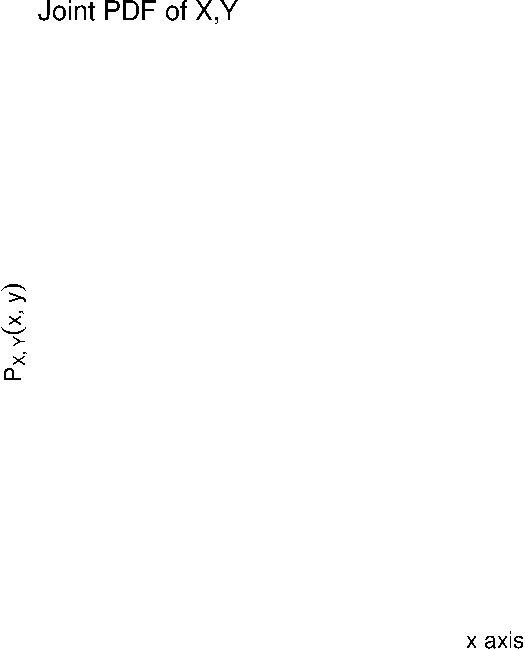
\includegraphics{06-hypothesis-testing_files/figure-pdf/unnamed-chunk-16-1.pdf}

\begin{Shaded}
\begin{Highlighting}[]
\NormalTok{home\_team }\SpecialCharTok{|\textgreater{}}  
  \FunctionTok{ggplot}\NormalTok{() }\SpecialCharTok{+} 
  \FunctionTok{aes}\NormalTok{(}\AttributeTok{x=}\FunctionTok{abs}\NormalTok{(score\_diff)) }\SpecialCharTok{+} 
  \FunctionTok{geom\_density}\NormalTok{()}
\end{Highlighting}
\end{Shaded}

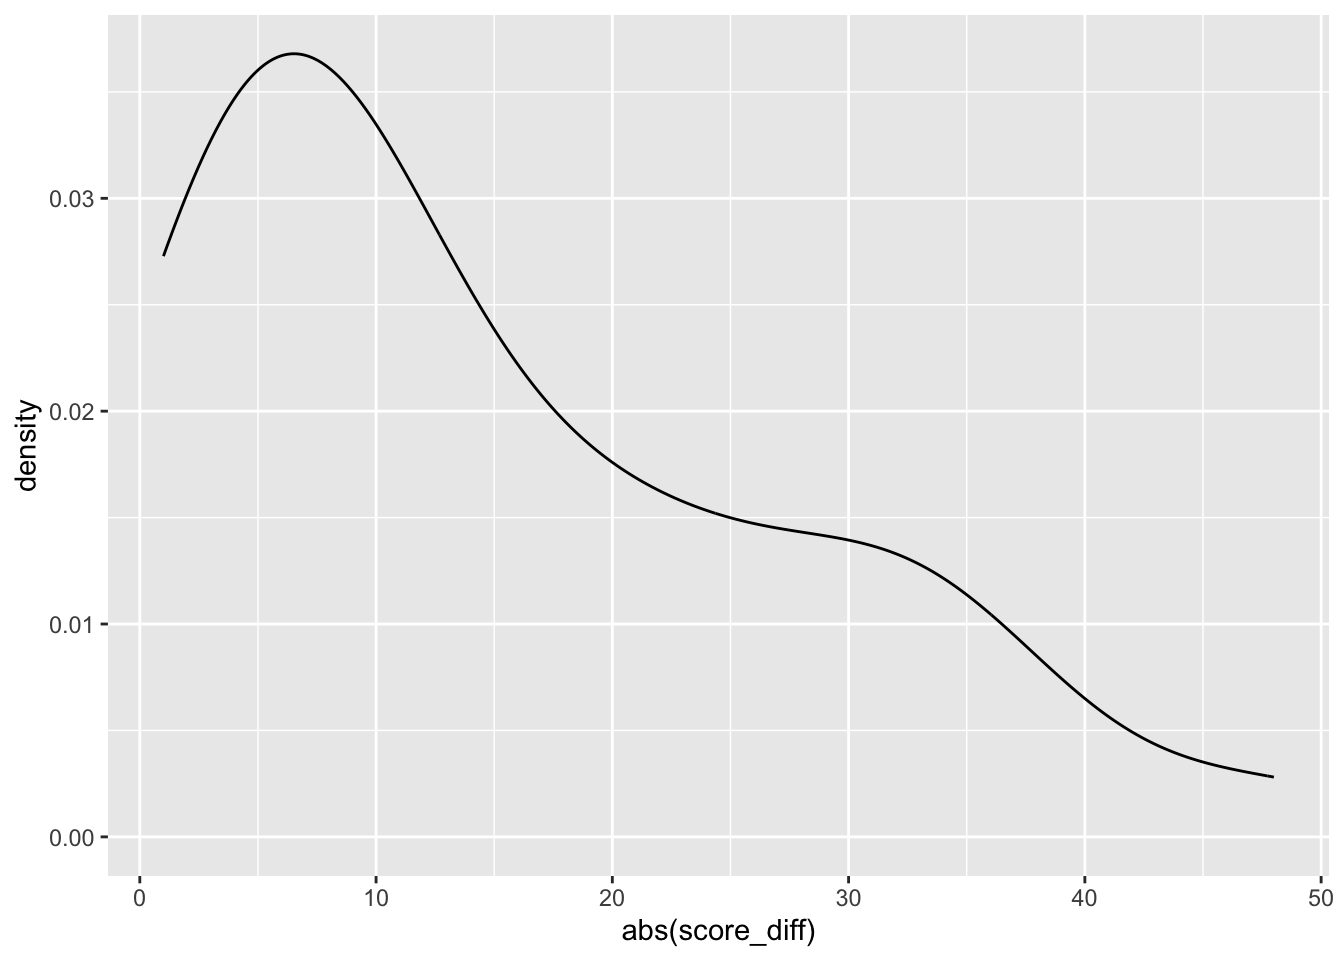
\includegraphics{06-hypothesis-testing_files/figure-pdf/unnamed-chunk-16-2.pdf}

\begin{Shaded}
\begin{Highlighting}[]
\FunctionTok{mean}\NormalTok{(home\_team}\SpecialCharTok{$}\NormalTok{score\_diff)}
\end{Highlighting}
\end{Shaded}

\begin{verbatim}
[1] -1.1
\end{verbatim}

\begin{Shaded}
\begin{Highlighting}[]
\FunctionTok{mean}\NormalTok{((res }\SpecialCharTok{\textless{}} \FunctionTok{mean}\NormalTok{(home\_team}\SpecialCharTok{$}\NormalTok{score\_diff))) }\SpecialCharTok{+} \FunctionTok{mean}\NormalTok{(res }\SpecialCharTok{\textgreater{}} \FunctionTok{abs}\NormalTok{(}\FunctionTok{mean}\NormalTok{(home\_team}\SpecialCharTok{$}\NormalTok{score\_diff)))}
\end{Highlighting}
\end{Shaded}

\begin{verbatim}
[1] 0.8868
\end{verbatim}

\begin{enumerate}
\def\labelenumi{\arabic{enumi}.}
\setcounter{enumi}{3}
\tightlist
\item
  Based on your output, suggest a different hypothesis that would have
  led to a different test result. Try executing the test to confirm that
  you are correct.
\end{enumerate}

\section{Assumptions Behind the
t-test}\label{assumptions-behind-the-t-test}

For the following scenarios, what is the strongest argument against the
validity of a t-test?

\begin{itemize}
\item
  You have a sample of 50 CEO salaries, and you want to know whether the
  mean salary is greater than \$1 million.
\item
  A nonprofit organization measures the percentage of students that pass
  an 8th grade reading test in 40 neighboring California counties. You
  are interested in whether the percentage of students that pass in
  California is over 80\%
\item
  You have survey data in which respondents assess their own opinion of
  corgis, with options ranging from ``1 - extreme disgust'' to ``5 -
  affection so intense it threatens my career.'' You want to know
  whether people on the average like corgis more than 3, representing
  neutrality.
\end{itemize}

\chapter{Comparing Two Groups}\label{comparing-two-groups}

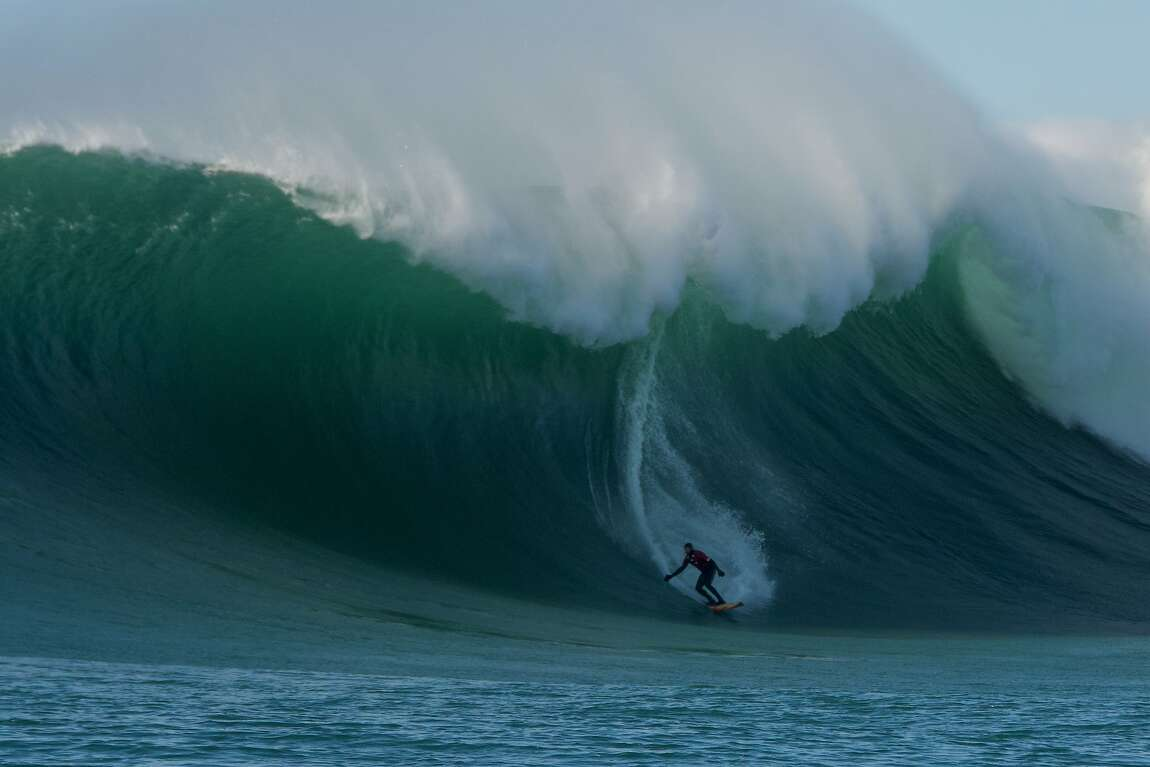
\includegraphics{./images/goin_left.jpeg}

\section{Learning Objectives}\label{learning-objectives-6}

This week, we introduce the idea of comparing two groups to evaluate
whether the data that we have sampled lead us to believe that the
population distribution of the random variables are different. Of
course, because we don't get access to the function that describes the
random variable, we can't \emph{actually} know if the populations are
different. It is for this reason that we call it statistical inference
-- we are inferring from a sample some belief about the populations.

At the conclusion of this week, students will be able to:

\begin{enumerate}
\def\labelenumi{\arabic{enumi}.}
\tightlist
\item
  \emph{Recognize} the similarities between all frequentist hypothesis
  tests.
\item
  \emph{Evaluate} the conditions that surround the data, and choose a
  test that is best-powered and justifiable.
\item
  \emph{Perform} and \emph{Interpret} the results of the most common
  statistical tests.
\end{enumerate}

\section{Class Announcements}\label{class-announcements-5}

\begin{itemize}
\tightlist
\item
  Great work completing your final w203 test!
\item
  Unit 7 Homework is Group Homework, due next week.
\item
  The Hypothesis Testing Lab is released today!

  \begin{itemize}
  \tightlist
  \item
    Lab is due at Unit 09 Live Session (two weeks): Apply these
    fundamentals to analyze 2022 election data and write a single,
    three-page analysis
  \end{itemize}
\end{itemize}

\section{Roadmap}\label{roadmap-3}

\subsection{Rearview Mirror}\label{rearview-mirror-1}

\begin{itemize}
\tightlist
\item
  Statisticians create a population model to represent the world
\item
  A population model has parameters we are interested in

  \begin{itemize}
  \tightlist
  \item
    Ex: A parameter might represent the effect that a vitamin has on
    test performance
  \end{itemize}
\item
  A null hypothesis is a specific statement about a parameter

  \begin{itemize}
  \tightlist
  \item
    Ex: The vitamin has zero effect on performance
  \end{itemize}
\item
  A hypothesis test is a procedure for rejecting or not rejecting a
  null, such the probability of a type 1 error is constrained.
\end{itemize}

\subsection{Today}\label{today}

\begin{itemize}
\tightlist
\item
  There are often multiple hypothesis tests you can apply to a scenario.
\item
  Our primary concern is choosing a test with assumptions we can defend.
\item
  Secondarily, we want to maximize power.
\end{itemize}

\subsection{Looking ahead}\label{looking-ahead}

\begin{itemize}
\tightlist
\item
  Next week, we start working with models for linear regression
\item
  We will see how hypothesis testing is also used for regression
  parameters.
\end{itemize}

\section{Teamwork Discussion}\label{teamwork-discussion}

\subsection{Working on Data Science
Teams}\label{working-on-data-science-teams}

Data science is a \emph{beautiful} combination of team-work and
individual-work. It provides the opportunity to work together on a data
pipeline with people from all over the organization, to deal with
technical, statistical, and social questions that are always
interesting. While we expect that everyone on a team will be a
professional, there is so much range within the pursuit of data science
that projects are nearly always collaborative exercises.

Together as teams, we

\begin{itemize}
\tightlist
\item
  Define research ambitions and scope
\item
  Imagine/envision the landscape of what is possible
\item
  Support, discuss, review and integrate individual contributions
\end{itemize}

Together as individuals we conduct the heads-down work that moves
question answering forward. This might be reading papers to determine
the most appropriate method to bring to bear on the question, or
researching the data that is available, or understanding the technical
requirements that we have to meet for this answer to be useful to our
organization in real time.

What is your instructor \emph{uniquely} capable of? Let them tell you!
But, at the same time, what would they acknowledge that others are
better than them?

See, the thing is, because there is so much that has to be done, there
literally are very, very few people who are one-stop data science shops.
Instead, teams rely on collaboration and joint expertise in order to get
good work done.

\subsection{The Problematic Psychology of Data
Science}\label{the-problematic-psychology-of-data-science}

People talk about the \emph{impostor syndrome}: a feeling of inadequacy
or interloping that is sometimes also associated with a fear of
under-performing relative to the expectation of others on the team.
These emotions are common through data science, academics, computer
science. But, these types of emotions are also commonplace in
journalism, film-making, and public speaking.

Has anybody ever had the dream that they're late to a test? Or, that
that they've got to give a speech that they're unprepared for? Does
anybody remember playing an instrument as a kid and having to go to
recitals? Or, play for a championship on a youth sports team? Or, go
into a test two?

What are the feelings associated with those events? What might be
generating these feelings?


\includegraphics[width=0.25\textwidth,height=\textheight]{images/among_us.jpeg}

\subsection{What Makes an Effective
Team?}\label{what-makes-an-effective-team}

\begin{itemize}
\tightlist
\item
  This reading on
  \href{https://rework.withgoogle.com/print/guides/5721312655835136/}{\emph{effective}
  teams} summarizes academic research to argue:
\end{itemize}

\begin{quote}
What really matters to creating an effective tema is less about who is
on the team, and more about how the team works together.
\end{quote}

In your live session, your section might take 7 minutes to read this
brief. If so, please read the following sections:

\begin{itemize}
\tightlist
\item
  The problem statement;
\item
  The proposed solution;
\item
  The framework for team effectiveness, stopping at the section titled
  \emph{``Tool: Help teams determine their own needs.''}
\end{itemize}

\begin{quote}
``Psychological safety refers to an individual's perception of the
consequences of taking an interpersonal risk. It is a belief that a team
is safe for risk taking in the face of being seen as ignorant,
incompetent, negative, or disruptive.''

``In a team with high psychological safety, teammates feel safe to take
risks around their team members. They feel confident that no one on the
team will embarrass or punish anyone else for admitting a mistake,
asking a question, or offering a new idea.''
\end{quote}

\subsection{We All Belong}\label{we-all-belong}

\begin{itemize}
\tightlist
\item
  From your experience, can you give an example of taking a personal
  risk as part of a team?

  \begin{itemize}
  \tightlist
  \item
    Can you describe your emotions when contemplating this risk?
  \item
    If you did take the risk, how did the reactions of your teammates
    affect you?
  \end{itemize}
\item
  Knowing the circumstances that generate feelings of anxiety -- what
  steps can we take as a section, or a team, to recognize and respond to
  these circumstances?
\end{itemize}

\begin{quote}
How can you add to the psychological safety of your peers in the section
and lab teammates?
\end{quote}

\section{Team Kick-Off}\label{team-kick-off}

\textbf{Lab 1 Teams}

\begin{itemize}
\tightlist
\item
  Here are teams for Lab 1!
\end{itemize}

\textbf{Team Kick-Off Conversation}

\begin{itemize}
\tightlist
\item
  In a 10 minute breakout with your team, please discuss the following
  questions:
\end{itemize}

\begin{enumerate}
\def\labelenumi{\arabic{enumi}.}
\tightlist
\item
  How much time will you invest in the lab each week?
\item
  How often will you meet and for how long?
\item
  How will you discuss, review, and integrate individual work into the
  team deliverable?
\item
  What do you see as the biggest risks when working on a team? How can
  you contribute to an effective team dynamic?
\end{enumerate}

\section{A Quick Review}\label{a-quick-review}

\textbf{Review of Key Terms}

\begin{itemize}
\tightlist
\item
  Define each of the following:

  \begin{itemize}
  \tightlist
  \item
    Population Parameter
  \item
    Null Hypothesis
  \item
    Test Statistic
  \item
    Null Distribution
  \end{itemize}
\end{itemize}

\textbf{Comparing Groups Review}

Take a moment to recall the tests you learned this week. Here is a quick
cheat-sheet to their key assumptions.

\begin{longtable}[]{@{}
  >{\raggedright\arraybackslash}p{(\columnwidth - 4\tabcolsep) * \real{0.1097}}
  >{\raggedright\arraybackslash}p{(\columnwidth - 4\tabcolsep) * \real{0.5226}}
  >{\raggedright\arraybackslash}p{(\columnwidth - 4\tabcolsep) * \real{0.3677}}@{}}
\toprule\noalign{}
\begin{minipage}[b]{\linewidth}\raggedright
paired/unpaired
\end{minipage} & \begin{minipage}[b]{\linewidth}\raggedright
parametric
\end{minipage} & \begin{minipage}[b]{\linewidth}\raggedright
non-parametric
\end{minipage} \\
\midrule\noalign{}
\endhead
\bottomrule\noalign{}
\endlastfoot
unpaired & \textbf{unpaired t-test} - metric var - i.i.d. - (not too
un-)normal & \textbf{Wilcoxon rank-sum} ordinal var i.i.d.  \\
paired & \textbf{paired t-test} metric var i.i.d. (not too un-)normal &
\textbf{Wilcoxon signed-rank} metric var i.i.d. difference is symmetric
\textbf{sign test} ordinal var i.i.d. \\
\end{longtable}

\section{Rank Based Tests}\label{rank-based-tests}

Darrin Speegle has a nice talk-through, walk through of rank based
testing procedures, linked
\href{https://bookdown.org/speegled/foundations-of-statistics/RBT.html\#two-sample-test}{here}.
We'll talk through a few examples of this, and then move to estimating
against data for the class.

\section{Comparing Groups R Exercise}\label{comparing-groups-r-exercise}

The General Social Survey (GSS) is one of the longest running and
extensive survey projects in the US. The full dataset includes over 1000
variables spanning demographics, attitudes, and behaviors. The file
\texttt{GSS\_w203.RData} contains a small selection of a variables from
the 2018 GSS.

To learn about each variable, you can enter it into the search bar at
the \href{https://gssdataexplorer.norc.org/variables/vfilter}{GSS data
explorer}

\begin{Shaded}
\begin{Highlighting}[]
\FunctionTok{load}\NormalTok{(}\StringTok{\textquotesingle{}data/GSS\_w203.RData\textquotesingle{}}\NormalTok{)}
\FunctionTok{summary}\NormalTok{(GSS)}
\end{Highlighting}
\end{Shaded}

\begin{verbatim}
           rincome               happy                           sexnow   
 $25000 or more: 851   very happy   : 701   women                   :758  
 $20000 - 24999: 107   pretty happy :1307   man                     :640  
 $10000 - 14999:  94   not too happy: 336   transgender             :  2  
 $15000 - 19999:  61   DK           :   0   a gender not listed here:  1  
 lt $1000      :  33   IAP          :   0   Don't know              :  0  
 (Other)       : 169   NA           :   0   (Other)                 :  0  
 NA's          :1033   NA's         :   4   NA's                    :947  
     wwwhr           emailhr                     socrel   
 Min.   :  0.00   Min.   :  0.000   sev times a week:382  
 1st Qu.:  3.00   1st Qu.:  0.000   sev times a mnth:287  
 Median :  8.00   Median :  2.000   once a month    :259  
 Mean   : 13.91   Mean   :  7.152   sev times a year:240  
 3rd Qu.: 20.00   3rd Qu.: 10.000   almost daily    :217  
 Max.   :140.00   Max.   :100.000   (Other)         :171  
 NA's   :986      NA's   :929       NA's            :792  
             socommun      numpets          tvhours      
 never           :510   Min.   : 0.000   Min.   : 0.000  
 once a month    :243   1st Qu.: 0.000   1st Qu.: 1.000  
 sev times a week:219   Median : 1.000   Median : 2.000  
 sev times a year:196   Mean   : 1.718   Mean   : 2.938  
 sev times a mnth:174   3rd Qu.: 2.000   3rd Qu.: 4.000  
 (Other)         :215   Max.   :20.000   Max.   :24.000  
 NA's            :791   NA's   :1201     NA's   :793     
                     major1         owngun   
 business administration: 138   yes    :537  
 education              :  79   no     :993  
 engineering            :  54   refused: 39  
 nursing                :  51   DK     :  0  
 health                 :  42   IAP    :  0  
 (Other)                : 546   NA     :  0  
 NA's                   :1438   NA's   :779  
\end{verbatim}

You have a set of questions that you would like to answer with a
statistical test. \textbf{For each question}:

\begin{enumerate}
\def\labelenumi{\arabic{enumi}.}
\tightlist
\item
  Choose the most appropriate test.
\item
  List and evaluate the assumptions for your test.
\item
  Conduct your test.
\item
  Discuss statistical and practical significance.
\end{enumerate}

\section{The Questions}\label{the-questions}

\subsection{Set 1}\label{set-1}

\begin{itemize}
\tightlist
\item
  Do economics majors watch more or less TV than computer science
  majors?
\end{itemize}

\begin{Shaded}
\begin{Highlighting}[]
\NormalTok{GSS }\SpecialCharTok{\%\textgreater{}\%} 
  \FunctionTok{filter}\NormalTok{(major1 }\SpecialCharTok{\%in\%} \FunctionTok{c}\NormalTok{(}\StringTok{\textquotesingle{}computer science\textquotesingle{}}\NormalTok{, }\StringTok{\textquotesingle{}economics\textquotesingle{}}\NormalTok{)) }\SpecialCharTok{\%\textgreater{}\%} 
  \FunctionTok{ggplot}\NormalTok{() }\SpecialCharTok{+} 
  \FunctionTok{aes}\NormalTok{(}\AttributeTok{x =}\NormalTok{ tvhours, }\AttributeTok{fill =}\NormalTok{ major1) }\SpecialCharTok{+} 
  \FunctionTok{geom\_histogram}\NormalTok{(}\AttributeTok{bins =} \DecValTok{10}\NormalTok{, }\AttributeTok{position =} \StringTok{\textquotesingle{}dodge\textquotesingle{}}\NormalTok{)}
\end{Highlighting}
\end{Shaded}

\begin{verbatim}
Warning: Removed 11 rows containing non-finite values (`stat_bin()`).
\end{verbatim}

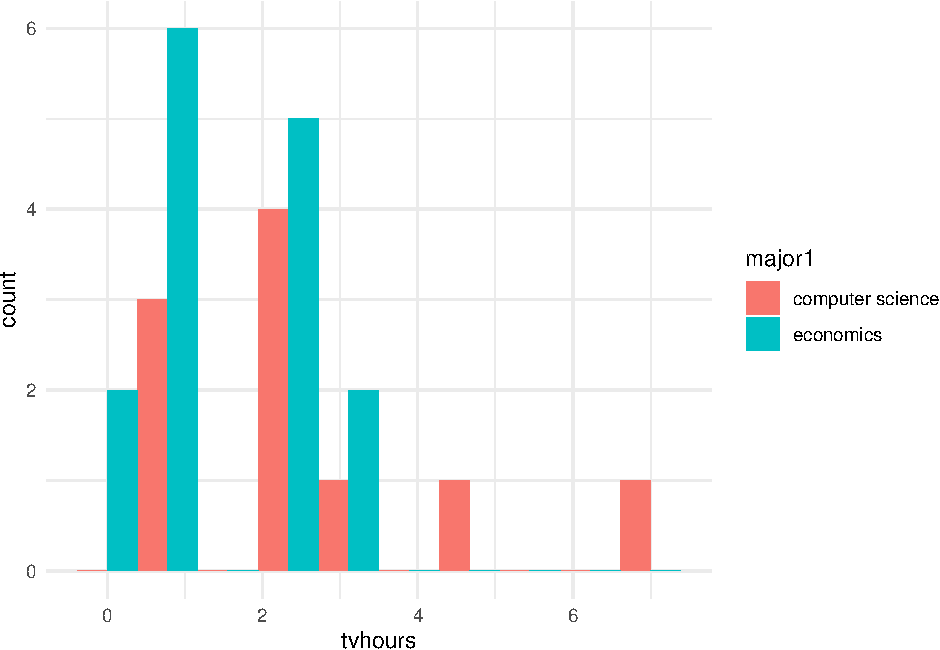
\includegraphics{07-comparing-two-groups_files/figure-pdf/plot relationship-1.pdf}

What kinds of tests \emph{could} be reasonable to conduct? For what part
of the data would we conduct these tests?

\begin{Shaded}
\begin{Highlighting}[]
\DocumentationTok{\#\# The assumptions about the data drive us to the correct test. }
\DocumentationTok{\#\# But, let\textquotesingle{}s ask all the tests that could *possibly* make sense, and see how }
\DocumentationTok{\#\#     matching or mis{-}matching assumptions changes what we learn. }

\DocumentationTok{\#\# Answers are in the next chunk... but don\textquotesingle{}t jump to them right away. }
\end{Highlighting}
\end{Shaded}

\begin{itemize}
\tightlist
\item
  Do Americans with pets watch more or less TV than Americans without
  pets?
\end{itemize}

\subsection{Set 2}\label{set-2}

\begin{itemize}
\tightlist
\item
  Do Americans spend more time emailing or using the web?
\end{itemize}

\begin{Shaded}
\begin{Highlighting}[]
\NormalTok{GSS }\SpecialCharTok{\%\textgreater{}\%} 
  \FunctionTok{select}\NormalTok{(wwwhr, emailhr) }\SpecialCharTok{\%\textgreater{}\%} 
  \FunctionTok{drop\_na}\NormalTok{() }\SpecialCharTok{\%$\%} 
  \FunctionTok{t.test}\NormalTok{(}\AttributeTok{x =}\NormalTok{ wwwhr, }\AttributeTok{y =}\NormalTok{ emailhr, }\AttributeTok{paired =} \ConstantTok{TRUE}\NormalTok{)}
\end{Highlighting}
\end{Shaded}

\begin{verbatim}

    Paired t-test

data:  wwwhr and emailhr
t = 13.44, df = 1360, p-value < 2.2e-16
alternative hypothesis: true mean difference is not equal to 0
95 percent confidence interval:
 5.530219 7.420553
sample estimates:
mean difference 
       6.475386 
\end{verbatim}

\begin{Shaded}
\begin{Highlighting}[]
\NormalTok{GSS }\SpecialCharTok{\%\textgreater{}\%} 
  \FunctionTok{ggplot}\NormalTok{() }\SpecialCharTok{+} 
  \FunctionTok{geom\_histogram}\NormalTok{(}\FunctionTok{aes}\NormalTok{(}\AttributeTok{x =}\NormalTok{ wwwhr),   }\AttributeTok{fill =} \StringTok{\textquotesingle{}darkblue\textquotesingle{}}\NormalTok{, }\AttributeTok{alpha =} \FloatTok{0.5}\NormalTok{) }\SpecialCharTok{+} 
  \FunctionTok{geom\_histogram}\NormalTok{(}\FunctionTok{aes}\NormalTok{(}\AttributeTok{x =}\NormalTok{ emailhr), }\AttributeTok{fill =} \StringTok{\textquotesingle{}darkred\textquotesingle{}}\NormalTok{,  }\AttributeTok{alpha =} \FloatTok{0.5}\NormalTok{)}
\end{Highlighting}
\end{Shaded}

\begin{verbatim}
`stat_bin()` using `bins = 30`. Pick better value with `binwidth`.
\end{verbatim}

\begin{verbatim}
Warning: Removed 986 rows containing non-finite values (`stat_bin()`).
\end{verbatim}

\begin{verbatim}
`stat_bin()` using `bins = 30`. Pick better value with `binwidth`.
\end{verbatim}

\begin{verbatim}
Warning: Removed 929 rows containing non-finite values (`stat_bin()`).
\end{verbatim}

\includegraphics{07-comparing-two-groups_files/figure-pdf/unnamed-chunk-5-1.pdf}

\begin{Shaded}
\begin{Highlighting}[]
\FunctionTok{t.test}\NormalTok{(}
  \AttributeTok{x =}\NormalTok{ GSS}\SpecialCharTok{$}\NormalTok{wwwhr, }
  \AttributeTok{y =}\NormalTok{ GSS}\SpecialCharTok{$}\NormalTok{emailhr, }
  \AttributeTok{paired =} \ConstantTok{FALSE}
\NormalTok{)}
\end{Highlighting}
\end{Shaded}

\begin{verbatim}

    Welch Two Sample t-test

data:  GSS$wwwhr and GSS$emailhr
t = 12.073, df = 2398.5, p-value < 2.2e-16
alternative hypothesis: true difference in means is not equal to 0
95 percent confidence interval:
 5.657397 7.851614
sample estimates:
mean of x mean of y 
13.906021  7.151515 
\end{verbatim}

\begin{itemize}
\tightlist
\item
  Do Americans spend more evenings with neighbors or with relatives?
\end{itemize}

\begin{Shaded}
\begin{Highlighting}[]
\NormalTok{wilcox\_test\_data }\OtherTok{\textless{}{-}}\NormalTok{ GSS }\SpecialCharTok{\%\textgreater{}\%} 
  \FunctionTok{select}\NormalTok{(socrel, socommun) }\SpecialCharTok{\%\textgreater{}\%}
  \FunctionTok{mutate}\NormalTok{(}
    \AttributeTok{family\_ordered =} \FunctionTok{factor}\NormalTok{(}
      \AttributeTok{x      =}\NormalTok{ socrel, }
      \AttributeTok{levels =} \FunctionTok{c}\NormalTok{(}\StringTok{\textquotesingle{}almost daily\textquotesingle{}}\NormalTok{, }\StringTok{\textquotesingle{}sev times a week\textquotesingle{}}\NormalTok{, }
                 \StringTok{\textquotesingle{}sev times a mnth\textquotesingle{}}\NormalTok{, }\StringTok{\textquotesingle{}once a month\textquotesingle{}}\NormalTok{,}
                 \StringTok{\textquotesingle{}sev times a year\textquotesingle{}}\NormalTok{, }\StringTok{\textquotesingle{}once a year\textquotesingle{}}\NormalTok{, }\StringTok{\textquotesingle{}never\textquotesingle{}}\NormalTok{)),}
    \AttributeTok{friends\_ordered =} \FunctionTok{factor}\NormalTok{(}
      \AttributeTok{x      =}\NormalTok{ socommun, }
      \AttributeTok{levels =} \FunctionTok{c}\NormalTok{(}\StringTok{\textquotesingle{}almost daily\textquotesingle{}}\NormalTok{, }\StringTok{\textquotesingle{}sev times a week\textquotesingle{}}\NormalTok{, }
                 \StringTok{\textquotesingle{}sev times a mnth\textquotesingle{}}\NormalTok{, }\StringTok{\textquotesingle{}once a month\textquotesingle{}}\NormalTok{,}
                 \StringTok{\textquotesingle{}sev times a year\textquotesingle{}}\NormalTok{, }\StringTok{\textquotesingle{}once a year\textquotesingle{}}\NormalTok{, }\StringTok{\textquotesingle{}never\textquotesingle{}}\NormalTok{))) }
\end{Highlighting}
\end{Shaded}

To begin this investigation, we've got to look at the data and see what
is in it. If you look below, you'll note that it sure seems that people
are spending more time with their family\ldots{} erp, actually no.
They're ``hanging out'' with their friends rather than taking their
mother out to dinner.

\begin{Shaded}
\begin{Highlighting}[]
\NormalTok{wilcox\_test\_data }\SpecialCharTok{\%\textgreater{}\%} 
  \FunctionTok{select}\NormalTok{(friends\_ordered, family\_ordered) }\SpecialCharTok{\%\textgreater{}\%} 
  \FunctionTok{rename}\NormalTok{(}
    \AttributeTok{Friends =}\NormalTok{ friends\_ordered, }
    \AttributeTok{Family  =}\NormalTok{ family\_ordered}
\NormalTok{  ) }\SpecialCharTok{\%\textgreater{}\%} 
  \FunctionTok{drop\_na}\NormalTok{() }\SpecialCharTok{\%\textgreater{}\%} 
  \FunctionTok{pivot\_longer}\NormalTok{(}\AttributeTok{cols =} \FunctionTok{c}\NormalTok{(Friends, Family)) }\SpecialCharTok{\%\textgreater{}\%}   
  \FunctionTok{ggplot}\NormalTok{() }\SpecialCharTok{+} 
    \FunctionTok{aes}\NormalTok{(}\AttributeTok{x=}\NormalTok{value, }\AttributeTok{fill=}\NormalTok{name) }\SpecialCharTok{+} 
    \FunctionTok{geom\_histogram}\NormalTok{(}\AttributeTok{stat=}\StringTok{\textquotesingle{}count\textquotesingle{}}\NormalTok{, }\AttributeTok{position=}\StringTok{\textquotesingle{}dodge\textquotesingle{}}\NormalTok{, }\AttributeTok{alpha=}\FloatTok{0.7}\NormalTok{) }\SpecialCharTok{+} 
  \FunctionTok{scale\_fill\_manual}\NormalTok{(}\AttributeTok{values =} \FunctionTok{c}\NormalTok{(}\StringTok{\textquotesingle{}\#003262\textquotesingle{}}\NormalTok{, }\StringTok{\textquotesingle{}\#FDB515\textquotesingle{}}\NormalTok{)) }\SpecialCharTok{+} 
  \FunctionTok{labs}\NormalTok{(}
    \AttributeTok{title    =} \StringTok{\textquotesingle{}Do Americans Spend Times With Friends or Family?\textquotesingle{}}\NormalTok{,}
    \AttributeTok{subtitle =} \StringTok{\textquotesingle{}A cutting analysis.\textquotesingle{}}\NormalTok{, }
    \AttributeTok{fill     =} \StringTok{\textquotesingle{}Friends or Family\textquotesingle{}}\NormalTok{, }
    \AttributeTok{x        =} \StringTok{\textquotesingle{}Amount of Time Spent\textquotesingle{}}\NormalTok{) }\SpecialCharTok{+} 
  \FunctionTok{scale\_x\_discrete}\NormalTok{(}\AttributeTok{guide =} \FunctionTok{guide\_axis}\NormalTok{(}\AttributeTok{n.dodge =} \DecValTok{2}\NormalTok{)) }\SpecialCharTok{+}
  \FunctionTok{theme\_minimal}\NormalTok{()}
\end{Highlighting}
\end{Shaded}

\begin{verbatim}
Warning in geom_histogram(stat = "count", position = "dodge", alpha = 0.7):
Ignoring unknown parameters: `binwidth`, `bins`, and `pad`
\end{verbatim}

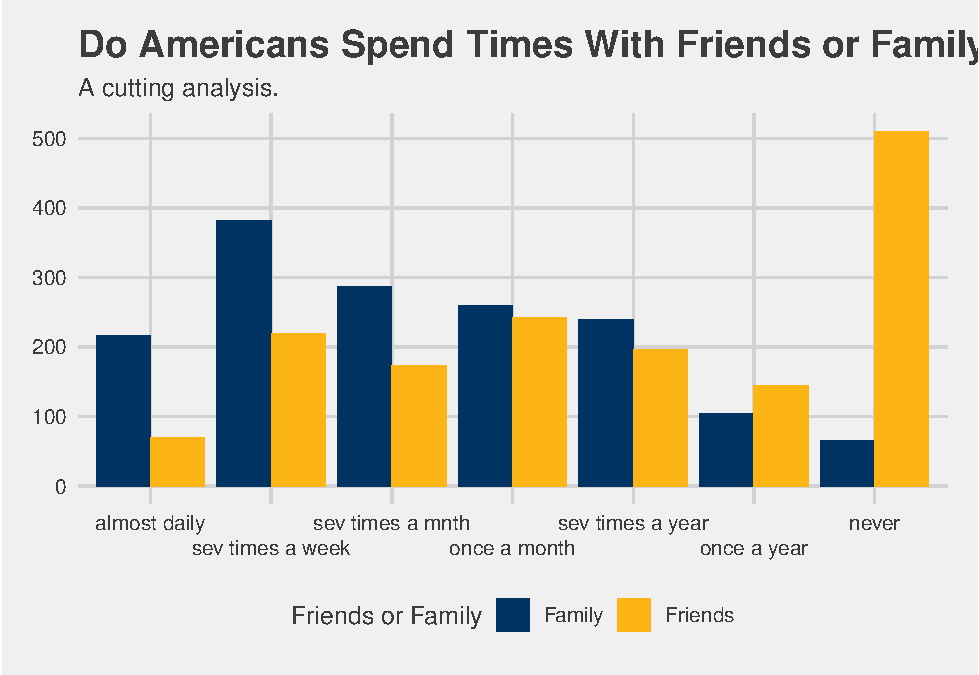
\includegraphics{07-comparing-two-groups_files/figure-pdf/produce descriptive plot-1.pdf}

With this plot created, we can ask if what we observe in the plot is the
produce of what could just be sampling error, or if this is something
that was unlikely to arise due if the null hypothesis were true. What is
the null hypothesis? Well, lets suppose that if we didn't know anything
about the data that we would expect there to be no difference between
the amount of time spent with friends or families.

\begin{Shaded}
\begin{Highlighting}[]
\DocumentationTok{\#\# risky choice {-}{-} casting the factor to a numeric without checking what happens.}
\NormalTok{wilcox\_test\_data }\SpecialCharTok{\%$\%} 
  \FunctionTok{wilcox.test}\NormalTok{(}
    \AttributeTok{x =} \FunctionTok{as.numeric}\NormalTok{(family\_ordered), }
    \AttributeTok{y =} \FunctionTok{as.numeric}\NormalTok{(friends\_ordered),}
    \AttributeTok{paired =} \ConstantTok{FALSE}
\NormalTok{  )}
\end{Highlighting}
\end{Shaded}

\begin{verbatim}

    Wilcoxon rank sum test with continuity correction

data:  as.numeric(family_ordered) and as.numeric(friends_ordered)
W = 716676, p-value < 2.2e-16
alternative hypothesis: true location shift is not equal to 0
\end{verbatim}

\subsection{Set 3}\label{set-3}

\begin{itemize}
\tightlist
\item
  Are Americans that own guns or Americans that don't own guns more
  likely to have pets?
\item
  Are Americans with pets happier than Americans without pets?
\end{itemize}

\subsection{Apply to a New Type of
Data}\label{apply-to-a-new-type-of-data}

\begin{itemize}
\tightlist
\item
  Is there a relationship between college major and gun ownership?
\end{itemize}

\section{Simulating the Effects of Test
Choices}\label{simulating-the-effects-of-test-choices}

\begin{Shaded}
\begin{Highlighting}[]
\FunctionTok{theme\_set}\NormalTok{(}\FunctionTok{theme\_minimal}\NormalTok{())}

\NormalTok{berkeley\_blue   }\OtherTok{\textless{}{-}} \StringTok{\textquotesingle{}\#003262\textquotesingle{}}
\NormalTok{berkeley\_gold   }\OtherTok{\textless{}{-}} \StringTok{\textquotesingle{}\#FDB515\textquotesingle{}}
\NormalTok{berkeley\_sather }\OtherTok{\textless{}{-}} \StringTok{\textquotesingle{}\#B9D3B6\textquotesingle{}}
\end{Highlighting}
\end{Shaded}

\subsection{Should we use a t-test or a wilcox
sign-rank?}\label{should-we-use-a-t-test-or-a-wilcox-sign-rank}

There is some open discussion in the applied statistics literature about
whether we should \emph{ever} be using a t-test. In particular, if the
underlying distribution that generates the data is \textbf{not} normal,
than the assumptions of a t-test are not, technically satisfied and the
test does not produce results that have nominal p-value coverage. This
is both \emph{technically} and \emph{theoretically} true; and yet,
researchers, data scientists, your instructors, and the entire world
runs t-tests as ``test of first recourse.''

What is the alternative to conducting a t-test as the test of first
recourse? It might be the Wilcox test. The Wilcox test makes a weaker
assumption -- of symmetry around the mean or median -- which is weaker
than the assumption of normality.

Additional points of argument, which you will investigate in this
worksheet:

\begin{itemize}
\tightlist
\item
  If the underlying data \textbf{is} normal, then the Wilcox test is
  \emph{nearly} as well powered as the t-test.
\item
  If the underlying data \textbf{is not} normal, then the Wilcox test
  still maintains nominal p-value coverage, whereas the t-test might
  lose this guarantee.
\end{itemize}

\section{}\label{section}

\subsection{The Poisson Distribution}\label{the-poisson-distribution}

The poisson distribution has the following PDF:

\[
f_X(x) = \frac{\lambda^n e^{-\lambda}}{n!}
\]

The key shape parameter for a poisson function is \(\lambda\); we show
three different distributions, setting this shape parameter to be 1, 3,
and 30 respectively. Notice that the limits on these plots are not set
to be the same; for example, the range in the third plot is considerably
larger than the first.

\begin{Shaded}
\begin{Highlighting}[]
\NormalTok{pois\_lambda\_1  }\OtherTok{\textless{}{-}} \FunctionTok{rpois}\NormalTok{(}\AttributeTok{n=}\DecValTok{1000}\NormalTok{, }\AttributeTok{lambda=}\DecValTok{1}\NormalTok{)}
\NormalTok{pois\_lambda\_3  }\OtherTok{\textless{}{-}} \FunctionTok{rpois}\NormalTok{(}\AttributeTok{n=}\DecValTok{1000}\NormalTok{, }\AttributeTok{lambda=}\DecValTok{3}\NormalTok{)}
\NormalTok{pois\_lambda\_30 }\OtherTok{\textless{}{-}} \FunctionTok{rpois}\NormalTok{(}\AttributeTok{n=}\DecValTok{1000}\NormalTok{, }\AttributeTok{lambda=}\DecValTok{30}\NormalTok{)}

\NormalTok{plot\_1  }\OtherTok{\textless{}{-}} \FunctionTok{ggplot}\NormalTok{() }\SpecialCharTok{+} \FunctionTok{aes}\NormalTok{(}\AttributeTok{x=}\NormalTok{pois\_lambda\_1) }\SpecialCharTok{+} \FunctionTok{geom\_histogram}\NormalTok{(}\AttributeTok{bins=}\DecValTok{6}\NormalTok{, }\AttributeTok{fill =}\NormalTok{ berkeley\_blue)}
\NormalTok{plot\_3  }\OtherTok{\textless{}{-}} \FunctionTok{ggplot}\NormalTok{() }\SpecialCharTok{+} \FunctionTok{aes}\NormalTok{(}\AttributeTok{x=}\NormalTok{pois\_lambda\_3) }\SpecialCharTok{+} \FunctionTok{geom\_histogram}\NormalTok{(}\AttributeTok{bins=}\DecValTok{10}\NormalTok{, }\AttributeTok{fill =}\NormalTok{ berkeley\_gold)}
\NormalTok{plot\_30 }\OtherTok{\textless{}{-}} \FunctionTok{ggplot}\NormalTok{() }\SpecialCharTok{+} \FunctionTok{aes}\NormalTok{(}\AttributeTok{x=}\NormalTok{pois\_lambda\_30) }\SpecialCharTok{+} \FunctionTok{geom\_histogram}\NormalTok{(}\AttributeTok{bins=}\DecValTok{30}\NormalTok{, }\AttributeTok{fill =}\NormalTok{ berkeley\_sather)}

\NormalTok{plot\_1 }\SpecialCharTok{/}\NormalTok{ plot\_3 }\SpecialCharTok{/}\NormalTok{ plot\_30}
\end{Highlighting}
\end{Shaded}

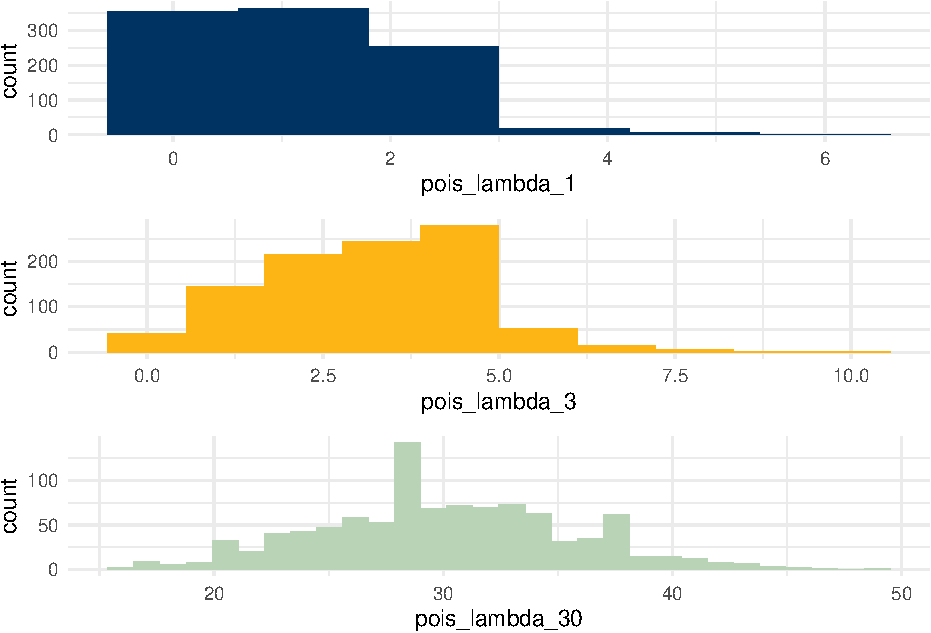
\includegraphics{07-comparing-two-groups_files/figure-pdf/show some from poisson distribution-1.pdf}

What does this changing distribution do to the p-values?

\subsection{Write a Simulation}\label{write-a-simulation}

\begin{Shaded}
\begin{Highlighting}[]
\NormalTok{pois\_sim }\OtherTok{\textless{}{-}} \ControlFlowTok{function}\NormalTok{(num\_observations, lambda\_one, lambda\_two) \{ }
  
\NormalTok{  t\_test\_result }\OtherTok{\textless{}{-}} \FunctionTok{rep}\NormalTok{(}\ConstantTok{NA}\NormalTok{, }\DecValTok{10000}\NormalTok{)}
\NormalTok{  wilcox\_result }\OtherTok{\textless{}{-}} \FunctionTok{rep}\NormalTok{(}\ConstantTok{NA}\NormalTok{, }\DecValTok{10000}\NormalTok{)}
  
  \ControlFlowTok{for}\NormalTok{(i }\ControlFlowTok{in} \DecValTok{1}\SpecialCharTok{:}\DecValTok{10000}\NormalTok{) \{ }
\NormalTok{    group\_one }\OtherTok{\textless{}{-}} \FunctionTok{rpois}\NormalTok{(}\AttributeTok{n=}\NormalTok{num\_observations, }\AttributeTok{lambda=}\NormalTok{lambda\_one)}
\NormalTok{    group\_two }\OtherTok{\textless{}{-}} \FunctionTok{rpois}\NormalTok{(}\AttributeTok{n=}\NormalTok{num\_observations, }\AttributeTok{lambda=}\NormalTok{lambda\_two)}
  
\NormalTok{    t\_test\_result[i] }\OtherTok{\textless{}{-}} \FunctionTok{t.test}\NormalTok{(group\_one, group\_two)}\SpecialCharTok{$}\NormalTok{p.value}
\NormalTok{    wilcox\_result[i] }\OtherTok{\textless{}{-}} \FunctionTok{wilcox.test}\NormalTok{(}\AttributeTok{x=}\NormalTok{group\_one, }\AttributeTok{y=}\NormalTok{group\_two)}\SpecialCharTok{$}\NormalTok{p.value}
\NormalTok{  \}}
  
\NormalTok{  df }\OtherTok{\textless{}{-}} \FunctionTok{data.table}\NormalTok{(}
    \AttributeTok{p\_value =} \FunctionTok{c}\NormalTok{(t\_test\_result, wilcox\_result), }
    \AttributeTok{test    =} \FunctionTok{rep}\NormalTok{(}\FunctionTok{c}\NormalTok{(}\StringTok{\textquotesingle{}t\_test\textquotesingle{}}\NormalTok{, }\StringTok{\textquotesingle{}wilcox\_test\textquotesingle{}}\NormalTok{), }\AttributeTok{each =} \DecValTok{10000}\NormalTok{)}
\NormalTok{  )}
  
  \FunctionTok{return}\NormalTok{(df)}
\NormalTok{\}}
\end{Highlighting}
\end{Shaded}

\begin{Shaded}
\begin{Highlighting}[]
\NormalTok{foo }\OtherTok{\textless{}{-}} \FunctionTok{pois\_sim}\NormalTok{(}\DecValTok{20}\NormalTok{, }\DecValTok{1}\NormalTok{, }\FloatTok{2.0}\NormalTok{)}
\end{Highlighting}
\end{Shaded}

\begin{Shaded}
\begin{Highlighting}[]
\NormalTok{foo }\SpecialCharTok{\%\textgreater{}\%}
  \FunctionTok{ggplot}\NormalTok{() }\SpecialCharTok{+}
  \FunctionTok{geom\_density}\NormalTok{(}\FunctionTok{aes}\NormalTok{(}\AttributeTok{x=}\NormalTok{p\_value, }\AttributeTok{color =}\NormalTok{ test)) }\SpecialCharTok{+}
  \FunctionTok{scale\_color\_manual}\NormalTok{(}\AttributeTok{values =} \FunctionTok{c}\NormalTok{(berkeley\_blue, berkeley\_gold))}
\end{Highlighting}
\end{Shaded}

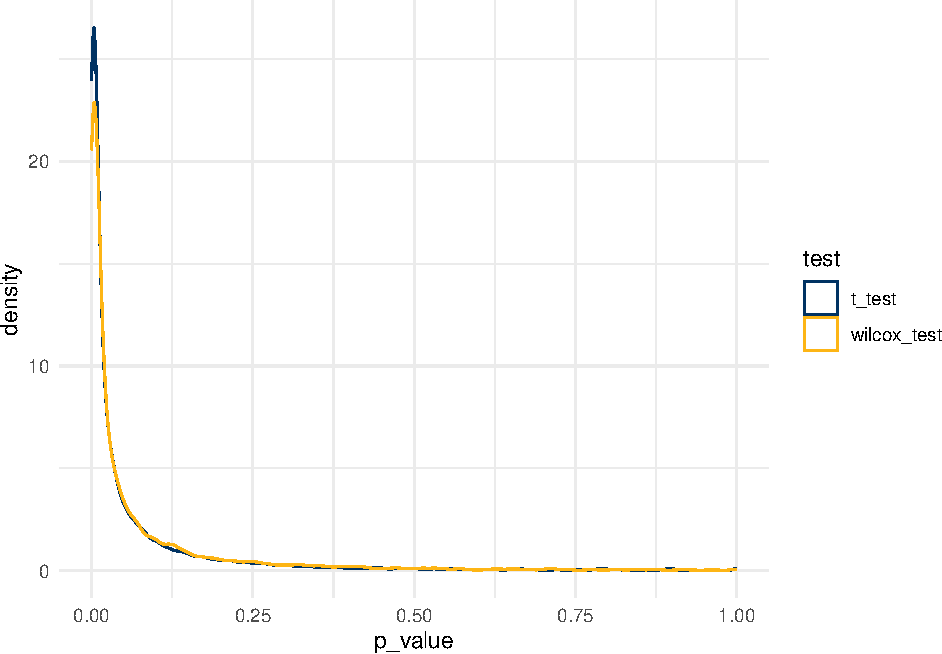
\includegraphics{07-comparing-two-groups_files/figure-pdf/plot results of simulation-1.pdf}

And so, the simulation rejects the null at the following rates:

\begin{itemize}
\tightlist
\item
  For the t-test, at a rate of 0.0667255
\item
  For the Wilcox test, at a rate of 0.0760637
\end{itemize}

\subsection{\texorpdfstring{What if a distribution is much \emph{more}
skewed?}{What if a distribution is much more skewed?}}\label{what-if-a-distribution-is-much-more-skewed}

\begin{Shaded}
\begin{Highlighting}[]
\NormalTok{skewed\_sim }\OtherTok{\textless{}{-}} \ControlFlowTok{function}\NormalTok{(}\AttributeTok{num\_sims=}\DecValTok{1000}\NormalTok{, num\_observations, alpha\_1, beta\_1, alpha\_2, beta\_2) \{}
  
\NormalTok{  t\_test\_result }\OtherTok{\textless{}{-}} \FunctionTok{rep}\NormalTok{(}\ConstantTok{NA}\NormalTok{, num\_sims)}
\NormalTok{  wilcox\_result }\OtherTok{\textless{}{-}} \FunctionTok{rep}\NormalTok{(}\ConstantTok{NA}\NormalTok{, num\_sims)}
  
  \ControlFlowTok{for}\NormalTok{(i }\ControlFlowTok{in} \DecValTok{1}\SpecialCharTok{:}\NormalTok{num\_sims) \{ }
\NormalTok{    group\_one }\OtherTok{\textless{}{-}} \FunctionTok{rbeta}\NormalTok{(}\AttributeTok{n=}\NormalTok{num\_observations, }\AttributeTok{shape1 =}\NormalTok{ alpha\_1, }\AttributeTok{shape2 =}\NormalTok{ beta\_1)}
\NormalTok{    group\_two }\OtherTok{\textless{}{-}} \FunctionTok{rbeta}\NormalTok{(}\AttributeTok{n=}\NormalTok{num\_observations, }\AttributeTok{shape1 =}\NormalTok{ alpha\_2, }\AttributeTok{shape2 =}\NormalTok{ beta\_2)}
  
\NormalTok{    t\_test\_result[i] }\OtherTok{\textless{}{-}} \FunctionTok{t.test}\NormalTok{(group\_one, group\_two)}\SpecialCharTok{$}\NormalTok{p.value}
\NormalTok{    wilcox\_result[i] }\OtherTok{\textless{}{-}} \FunctionTok{wilcox.test}\NormalTok{(}\AttributeTok{x=}\NormalTok{group\_one, }\AttributeTok{y=}\NormalTok{group\_two)}\SpecialCharTok{$}\NormalTok{p.value}
\NormalTok{  \}}
  
\NormalTok{  dt }\OtherTok{\textless{}{-}} \FunctionTok{data.table}\NormalTok{(}
    \AttributeTok{p\_value =} \FunctionTok{c}\NormalTok{(t\_test\_result, wilcox\_result), }
    \AttributeTok{test    =} \FunctionTok{rep}\NormalTok{(}\FunctionTok{c}\NormalTok{(}\StringTok{\textquotesingle{}t\_test\textquotesingle{}}\NormalTok{, }\StringTok{\textquotesingle{}wilcox\_test\textquotesingle{}}\NormalTok{), }\AttributeTok{each =}\NormalTok{ num\_sims)}
\NormalTok{  )}
  
  \FunctionTok{return}\NormalTok{(dt)}
\NormalTok{\}}
\end{Highlighting}
\end{Shaded}

\subsection{False Rejection Rates}\label{false-rejection-rates}

Start with a distribution that has parameters \texttt{alpha=2},
\texttt{beta=7}.

\begin{Shaded}
\begin{Highlighting}[]
\FunctionTok{ggplot}\NormalTok{(}\FunctionTok{data.frame}\NormalTok{(}\AttributeTok{x=}\FunctionTok{c}\NormalTok{(}\DecValTok{0}\NormalTok{,}\DecValTok{1}\NormalTok{)), }\FunctionTok{aes}\NormalTok{(x)) }\SpecialCharTok{+} 
  \FunctionTok{stat\_function}\NormalTok{(}\AttributeTok{fun =}\NormalTok{ dbeta, }\AttributeTok{n=}\DecValTok{100}\NormalTok{, }\AttributeTok{args=}\FunctionTok{list}\NormalTok{(}\AttributeTok{shape1=}\DecValTok{2}\NormalTok{, }\AttributeTok{shape2=}\DecValTok{7}\NormalTok{))}
\end{Highlighting}
\end{Shaded}

\includegraphics{07-comparing-two-groups_files/figure-pdf/unnamed-chunk-8-1.pdf}

\begin{Shaded}
\begin{Highlighting}[]
\NormalTok{same\_dist\_small\_data }\OtherTok{\textless{}{-}} \FunctionTok{skewed\_sim}\NormalTok{(}
  \AttributeTok{num\_observations=}\DecValTok{10}\NormalTok{, }
  \AttributeTok{alpha\_1=}\DecValTok{2}\NormalTok{, }\AttributeTok{beta\_1=}\DecValTok{7}\NormalTok{, }
  \AttributeTok{alpha\_2=}\DecValTok{2}\NormalTok{, }\AttributeTok{beta\_2=}\DecValTok{7}
\NormalTok{  )}
\NormalTok{same\_dist\_med\_data }\OtherTok{\textless{}{-}} \FunctionTok{skewed\_sim}\NormalTok{(}
  \AttributeTok{num\_observations=}\DecValTok{50}\NormalTok{, }
  \AttributeTok{alpha\_1=}\DecValTok{2}\NormalTok{, }\AttributeTok{beta\_1=}\DecValTok{7}\NormalTok{, }
  \AttributeTok{alpha\_2=}\DecValTok{2}\NormalTok{, }\AttributeTok{beta\_2=}\DecValTok{7}
\NormalTok{  )}
\NormalTok{same\_dist\_big\_data }\OtherTok{\textless{}{-}} \FunctionTok{skewed\_sim}\NormalTok{( }\CommentTok{\# haha, "big data"}
  \AttributeTok{num\_observations=}\DecValTok{100}\NormalTok{, }
  \AttributeTok{alpha\_1=}\DecValTok{2}\NormalTok{, }\AttributeTok{beta\_1=}\DecValTok{7}\NormalTok{, }
  \AttributeTok{alpha\_2=}\DecValTok{2}\NormalTok{, }\AttributeTok{beta\_2=}\DecValTok{7}
\NormalTok{  )}
\end{Highlighting}
\end{Shaded}

\begin{Shaded}
\begin{Highlighting}[]
\NormalTok{plot\_1 }\OtherTok{\textless{}{-}}\NormalTok{ same\_dist\_small\_data }\SpecialCharTok{\%\textgreater{}\%}
  \FunctionTok{ggplot}\NormalTok{() }\SpecialCharTok{+}
  \FunctionTok{geom\_density}\NormalTok{(}\FunctionTok{aes}\NormalTok{(}\AttributeTok{x=}\NormalTok{p\_value, }\AttributeTok{color =}\NormalTok{ test), }\AttributeTok{bounds=}\FunctionTok{c}\NormalTok{(}\DecValTok{0}\NormalTok{,}\DecValTok{1}\NormalTok{)) }\SpecialCharTok{+}
  \FunctionTok{scale\_color\_manual}\NormalTok{(}\AttributeTok{values =} \FunctionTok{c}\NormalTok{(berkeley\_blue, berkeley\_gold))}
\NormalTok{plot\_2 }\OtherTok{\textless{}{-}}\NormalTok{ same\_dist\_med\_data }\SpecialCharTok{\%\textgreater{}\%}
  \FunctionTok{ggplot}\NormalTok{() }\SpecialCharTok{+}
  \FunctionTok{geom\_density}\NormalTok{(}\FunctionTok{aes}\NormalTok{(}\AttributeTok{x=}\NormalTok{p\_value, }\AttributeTok{color =}\NormalTok{ test), }\AttributeTok{bounds=}\FunctionTok{c}\NormalTok{(}\DecValTok{0}\NormalTok{,}\DecValTok{1}\NormalTok{)) }\SpecialCharTok{+}
  \FunctionTok{scale\_color\_manual}\NormalTok{(}\AttributeTok{values =} \FunctionTok{c}\NormalTok{(berkeley\_blue, berkeley\_gold))}
\NormalTok{plot\_3 }\OtherTok{\textless{}{-}}\NormalTok{ same\_dist\_big\_data }\SpecialCharTok{\%\textgreater{}\%}
  \FunctionTok{ggplot}\NormalTok{() }\SpecialCharTok{+}
  \FunctionTok{geom\_density}\NormalTok{(}\FunctionTok{aes}\NormalTok{(}\AttributeTok{x=}\NormalTok{p\_value, }\AttributeTok{color =}\NormalTok{ test), }\AttributeTok{bounds=}\FunctionTok{c}\NormalTok{(}\DecValTok{0}\NormalTok{,}\DecValTok{1}\NormalTok{)) }\SpecialCharTok{+}
  \FunctionTok{scale\_color\_manual}\NormalTok{(}\AttributeTok{values =} \FunctionTok{c}\NormalTok{(berkeley\_blue, berkeley\_gold))}

\NormalTok{plot\_1 }\SpecialCharTok{/}\NormalTok{ plot\_2 }\SpecialCharTok{/}\NormalTok{ plot\_3}
\end{Highlighting}
\end{Shaded}

\includegraphics{07-comparing-two-groups_files/figure-pdf/unnamed-chunk-10-1.pdf}

\begin{itemize}
\tightlist
\item
  T-tests

  \begin{itemize}
  \tightlist
  \item
    0.042
  \item
    0.047
  \item
    0.065
  \end{itemize}
\item
  Wilcox Tests

  \begin{itemize}
  \tightlist
  \item
    0.036
  \item
    0.036
  \item
    0.056
  \end{itemize}
\end{itemize}

\subsection{What about Power to
Reject}\label{what-about-power-to-reject}

\begin{Shaded}
\begin{Highlighting}[]
\NormalTok{small\_diff\_small\_data }\OtherTok{\textless{}{-}} \FunctionTok{skewed\_sim}\NormalTok{(}
  \AttributeTok{num\_observations=}\DecValTok{10}\NormalTok{, }
  \AttributeTok{alpha\_1=}\DecValTok{2}\NormalTok{, }\AttributeTok{beta\_1=}\DecValTok{7}\NormalTok{, }
  \AttributeTok{alpha\_2=}\DecValTok{2}\NormalTok{, }\AttributeTok{beta\_2=}\DecValTok{5}
\NormalTok{  )}
\NormalTok{small\_diff\_med\_data }\OtherTok{\textless{}{-}} \FunctionTok{skewed\_sim}\NormalTok{(}
  \AttributeTok{num\_observations=}\DecValTok{50}\NormalTok{, }
  \AttributeTok{alpha\_1=}\DecValTok{2}\NormalTok{, }\AttributeTok{beta\_1=}\DecValTok{7}\NormalTok{, }
  \AttributeTok{alpha\_2=}\DecValTok{2}\NormalTok{, }\AttributeTok{beta\_2=}\DecValTok{5}
\NormalTok{  )}
\NormalTok{small\_diff\_big\_data }\OtherTok{\textless{}{-}} \FunctionTok{skewed\_sim}\NormalTok{( }\CommentTok{\# haha, "big data"}
  \AttributeTok{num\_observations=}\DecValTok{100}\NormalTok{, }
  \AttributeTok{alpha\_1=}\DecValTok{2}\NormalTok{, }\AttributeTok{beta\_1=}\DecValTok{7}\NormalTok{, }
  \AttributeTok{alpha\_2=}\DecValTok{2}\NormalTok{, }\AttributeTok{beta\_2=}\DecValTok{5}
\NormalTok{  )}
\end{Highlighting}
\end{Shaded}

\begin{Shaded}
\begin{Highlighting}[]
\NormalTok{plot\_1 }\OtherTok{\textless{}{-}}\NormalTok{ small\_diff\_small\_data }\SpecialCharTok{\%\textgreater{}\%}
  \FunctionTok{ggplot}\NormalTok{() }\SpecialCharTok{+}
  \FunctionTok{geom\_density}\NormalTok{(}\FunctionTok{aes}\NormalTok{(}\AttributeTok{x=}\NormalTok{p\_value, }\AttributeTok{color =}\NormalTok{ test), }\AttributeTok{bounds=}\FunctionTok{c}\NormalTok{(}\DecValTok{0}\NormalTok{,}\DecValTok{1}\NormalTok{)) }\SpecialCharTok{+}
  \FunctionTok{scale\_color\_manual}\NormalTok{(}\AttributeTok{values =} \FunctionTok{c}\NormalTok{(berkeley\_blue, berkeley\_gold))}
\NormalTok{plot\_2 }\OtherTok{\textless{}{-}}\NormalTok{ small\_diff\_med\_data }\SpecialCharTok{\%\textgreater{}\%}
  \FunctionTok{ggplot}\NormalTok{() }\SpecialCharTok{+}
  \FunctionTok{geom\_density}\NormalTok{(}\FunctionTok{aes}\NormalTok{(}\AttributeTok{x=}\NormalTok{p\_value, }\AttributeTok{color =}\NormalTok{ test), }\AttributeTok{bounds=}\FunctionTok{c}\NormalTok{(}\DecValTok{0}\NormalTok{,}\DecValTok{1}\NormalTok{)) }\SpecialCharTok{+}
  \FunctionTok{scale\_color\_manual}\NormalTok{(}\AttributeTok{values =} \FunctionTok{c}\NormalTok{(berkeley\_blue, berkeley\_gold))}
\NormalTok{plot\_3 }\OtherTok{\textless{}{-}}\NormalTok{ small\_diff\_big\_data }\SpecialCharTok{\%\textgreater{}\%}
  \FunctionTok{ggplot}\NormalTok{() }\SpecialCharTok{+}
  \FunctionTok{geom\_density}\NormalTok{(}\FunctionTok{aes}\NormalTok{(}\AttributeTok{x=}\NormalTok{p\_value, }\AttributeTok{color =}\NormalTok{ test), }\AttributeTok{bounds=}\FunctionTok{c}\NormalTok{(}\DecValTok{0}\NormalTok{,}\DecValTok{1}\NormalTok{)) }\SpecialCharTok{+}
  \FunctionTok{scale\_color\_manual}\NormalTok{(}\AttributeTok{values =} \FunctionTok{c}\NormalTok{(berkeley\_blue, berkeley\_gold))}

\NormalTok{plot\_1 }\SpecialCharTok{/}\NormalTok{ plot\_2 }\SpecialCharTok{/}\NormalTok{ plot\_3}
\end{Highlighting}
\end{Shaded}

\includegraphics{07-comparing-two-groups_files/figure-pdf/unnamed-chunk-12-1.pdf}

\subsection{Paired compared to unpaired
tests}\label{paired-compared-to-unpaired-tests}

\begin{Shaded}
\begin{Highlighting}[]
\NormalTok{paired\_sim }\OtherTok{\textless{}{-}} \ControlFlowTok{function}\NormalTok{(}\AttributeTok{num\_sims=}\DecValTok{10000}\NormalTok{, num\_observations, mean\_one, mean\_two, paired\_diff, sd\_one, sd\_two) \{ }
  
\NormalTok{  unpaired\_test\_unpaired\_data }\OtherTok{\textless{}{-}} \FunctionTok{rep}\NormalTok{(}\ConstantTok{NA}\NormalTok{, num\_sims)}
\NormalTok{  unpaired\_test\_paired\_data   }\OtherTok{\textless{}{-}} \FunctionTok{rep}\NormalTok{(}\ConstantTok{NA}\NormalTok{, num\_sims)}
\NormalTok{  paired\_test\_unpaired\_data   }\OtherTok{\textless{}{-}} \FunctionTok{rep}\NormalTok{(}\ConstantTok{NA}\NormalTok{, num\_sims)}
\NormalTok{  paired\_test\_paired\_data     }\OtherTok{\textless{}{-}} \FunctionTok{rep}\NormalTok{(}\ConstantTok{NA}\NormalTok{, num\_sims)}
  
  \ControlFlowTok{for}\NormalTok{(i }\ControlFlowTok{in} \DecValTok{1}\SpecialCharTok{:}\NormalTok{num\_sims) \{ }
\NormalTok{    observation\_a1 }\OtherTok{\textless{}{-}} \FunctionTok{rnorm}\NormalTok{(}\AttributeTok{n =}\NormalTok{ num\_observations, }\AttributeTok{mean =}\NormalTok{ mean\_one, }\AttributeTok{sd =}\NormalTok{ sd\_one) }
    \DocumentationTok{\#\# first create unpaired data }
\NormalTok{    observation\_b }\OtherTok{\textless{}{-}} \FunctionTok{rnorm}\NormalTok{(}\AttributeTok{n =}\NormalTok{ num\_observations, }\AttributeTok{mean =}\NormalTok{ mean\_two, }\AttributeTok{sd =}\NormalTok{ sd\_two)}
    \DocumentationTok{\#\# then, create paired data }
\NormalTok{    observation\_a2 }\OtherTok{\textless{}{-}}\NormalTok{ observation\_a1 }\SpecialCharTok{+} \FunctionTok{rnorm}\NormalTok{(}\AttributeTok{n =}\NormalTok{ num\_observations, }\AttributeTok{mean =}\NormalTok{ paired\_diff, }\AttributeTok{sd=}\NormalTok{sd\_two)}
    
    \DocumentationTok{\#\# run tests}
\NormalTok{    unpaired\_test\_unpaired\_data[i] }\OtherTok{\textless{}{-}} \FunctionTok{t.test}\NormalTok{(}\AttributeTok{x=}\NormalTok{observation\_a1, }\AttributeTok{y=}\NormalTok{observation\_b,  }\AttributeTok{paired=}\ConstantTok{FALSE}\NormalTok{)}\SpecialCharTok{$}\NormalTok{p.value}
\NormalTok{    unpaired\_test\_paired\_data[i]   }\OtherTok{\textless{}{-}} \FunctionTok{t.test}\NormalTok{(}\AttributeTok{x=}\NormalTok{observation\_a1, }\AttributeTok{y=}\NormalTok{observation\_a2,  }\AttributeTok{paired=}\ConstantTok{FALSE}\NormalTok{)}\SpecialCharTok{$}\NormalTok{p.value}
\NormalTok{    paired\_test\_unpaired\_data[i]   }\OtherTok{\textless{}{-}} \FunctionTok{t.test}\NormalTok{(}\AttributeTok{x=}\NormalTok{observation\_a1, }\AttributeTok{y=}\NormalTok{observation\_b,  }\AttributeTok{paired=}\ConstantTok{TRUE}\NormalTok{)}\SpecialCharTok{$}\NormalTok{p.value}
\NormalTok{    paired\_test\_paired\_data[i]     }\OtherTok{\textless{}{-}} \FunctionTok{t.test}\NormalTok{(}\AttributeTok{x=}\NormalTok{observation\_a1, }\AttributeTok{y=}\NormalTok{observation\_a2, }\AttributeTok{paired=}\ConstantTok{TRUE}\NormalTok{)}\SpecialCharTok{$}\NormalTok{p.value}
\NormalTok{  \}}
  
\NormalTok{  dt }\OtherTok{\textless{}{-}} \FunctionTok{data.table}\NormalTok{(}
    \AttributeTok{p\_value =} \FunctionTok{c}\NormalTok{(unpaired\_test\_unpaired\_data, unpaired\_test\_paired\_data, }
\NormalTok{                paired\_test\_unpaired\_data,   paired\_test\_paired\_data), }
    \AttributeTok{test    =} \FunctionTok{rep}\NormalTok{(}\FunctionTok{c}\NormalTok{(}\StringTok{\textquotesingle{}unpaired data, unpaired test\textquotesingle{}}\NormalTok{, }\StringTok{\textquotesingle{}paired data, unpaired test\textquotesingle{}}\NormalTok{, }
                    \StringTok{\textquotesingle{}unpaired data, paired test\textquotesingle{}}\NormalTok{, }\StringTok{\textquotesingle{}paired data, paired test\textquotesingle{}}\NormalTok{), }\AttributeTok{each =}\NormalTok{ num\_sims)}
\NormalTok{  )}
  
  \FunctionTok{return}\NormalTok{(dt)}
\NormalTok{\}}
\end{Highlighting}
\end{Shaded}

\begin{Shaded}
\begin{Highlighting}[]
\NormalTok{bar }\OtherTok{\textless{}{-}} \FunctionTok{paired\_sim}\NormalTok{(}\AttributeTok{num\_observations =} \DecValTok{30}\NormalTok{,  }\AttributeTok{mean\_one =} \DecValTok{10}\NormalTok{, }\AttributeTok{mean\_two =} \DecValTok{11}\NormalTok{, }\AttributeTok{paired\_diff =} \DecValTok{1}\NormalTok{, }\AttributeTok{sd\_one =} \DecValTok{4}\NormalTok{, }\AttributeTok{sd\_two =} \DecValTok{5}\NormalTok{)}
\end{Highlighting}
\end{Shaded}

\begin{Shaded}
\begin{Highlighting}[]
\NormalTok{paired\_data\_plot }\OtherTok{\textless{}{-}}\NormalTok{ bar[}\FunctionTok{grep}\NormalTok{(}\StringTok{\textquotesingle{}unpaired data\textquotesingle{}}\NormalTok{, test, }\AttributeTok{invert=}\ConstantTok{TRUE}\NormalTok{)] }\SpecialCharTok{\%\textgreater{}\%} 
  \FunctionTok{ggplot}\NormalTok{() }\SpecialCharTok{+} 
    \FunctionTok{aes}\NormalTok{(}\AttributeTok{x=}\NormalTok{p\_value, }\AttributeTok{color =}\NormalTok{ test, }\AttributeTok{fill =}\NormalTok{ test) }\SpecialCharTok{+} 
    \FunctionTok{geom\_density}\NormalTok{(}\AttributeTok{alpha=}\FloatTok{0.25}\NormalTok{) }\SpecialCharTok{+} 
  \FunctionTok{labs}\NormalTok{(}\AttributeTok{title =} \StringTok{\textquotesingle{}Paired Data\textquotesingle{}}\NormalTok{)}
\NormalTok{unpaired\_data\_plot }\OtherTok{\textless{}{-}}\NormalTok{ bar[}\FunctionTok{grep}\NormalTok{(}\StringTok{\textquotesingle{}unpaired data\textquotesingle{}}\NormalTok{, test, }\AttributeTok{invert=}\ConstantTok{FALSE}\NormalTok{)] }\SpecialCharTok{\%\textgreater{}\%} 
  \FunctionTok{ggplot}\NormalTok{() }\SpecialCharTok{+} 
    \FunctionTok{aes}\NormalTok{(}\AttributeTok{x=}\NormalTok{p\_value, }\AttributeTok{color =}\NormalTok{ test, }\AttributeTok{fill =}\NormalTok{ test) }\SpecialCharTok{+} 
    \FunctionTok{geom\_density}\NormalTok{(}\AttributeTok{alpha=}\FloatTok{0.25}\NormalTok{) }\SpecialCharTok{+} 
  \FunctionTok{labs}\NormalTok{(}\AttributeTok{title =} \StringTok{\textquotesingle{}Unpaired Data\textquotesingle{}}\NormalTok{)}

\NormalTok{paired\_data\_plot }\SpecialCharTok{/}\NormalTok{ unpaired\_data\_plot}
\end{Highlighting}
\end{Shaded}

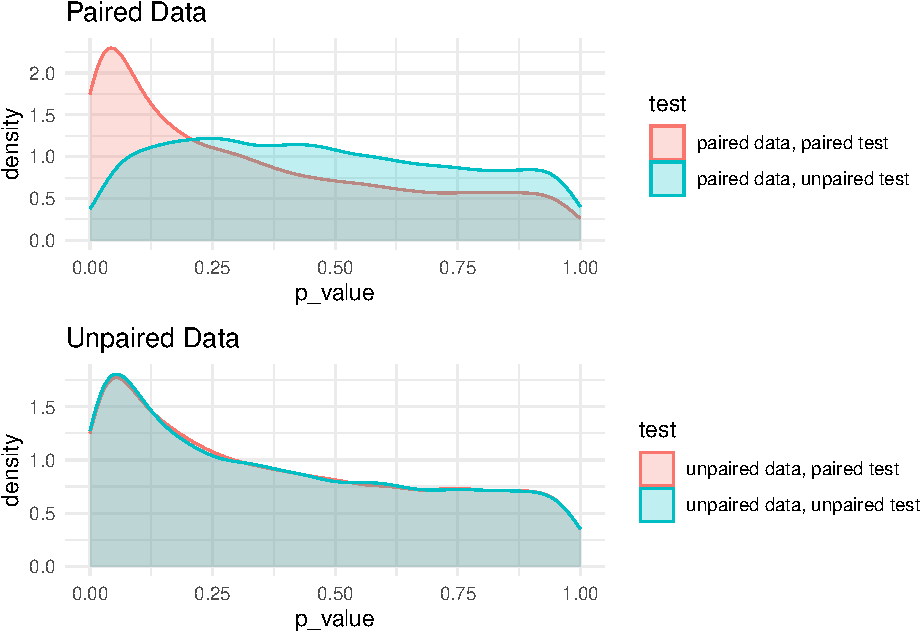
\includegraphics{07-comparing-two-groups_files/figure-pdf/plot results of paired simulation-1.pdf}

\part{Regression}

In this section, we talk about regression. There is much talk about
regression.

\chapter{OLS Regression Estimates}\label{ols-regression-estimates}

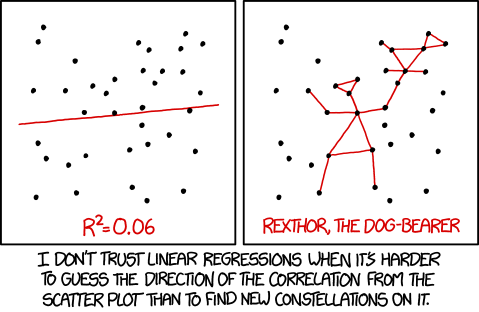
\includegraphics{./images/linear_regression.png}

\begin{Shaded}
\begin{Highlighting}[]
\FunctionTok{library}\NormalTok{(tidyverse)}
\FunctionTok{library}\NormalTok{(broom)}
\FunctionTok{library}\NormalTok{(testthat)}
\FunctionTok{library}\NormalTok{(patchwork)}
\end{Highlighting}
\end{Shaded}

\begin{Shaded}
\begin{Highlighting}[]
\FunctionTok{theme\_set}\NormalTok{(}\FunctionTok{theme\_minimal}\NormalTok{())}
\end{Highlighting}
\end{Shaded}

\section{Learning Objectives}\label{learning-objectives-7}

At the end of this week, students will be able to:

\begin{enumerate}
\def\labelenumi{\arabic{enumi}.}
\tightlist
\item
  \textbf{Understand} the algorithm that produces the OLS regression
  estimates.
\item
  \textbf{Fit} regressions to produce estimates from a best linear
  predictor.
\item
  \textbf{Produce} predictions from this OLS regression that are
  informative about the population.
\end{enumerate}

\section{Class Announcements}\label{class-announcements-6}

\begin{enumerate}
\def\labelenumi{\arabic{enumi}.}
\tightlist
\item
  Lab 1 is due next week!
\item
  There is not a ``homework'' assignment this week -- instead you're
  working on your group's lab
\item
  You're doing great - keep it up!
\end{enumerate}

\section{Roadmap}\label{roadmap-4}

\textbf{Rear-View Mirror}

\begin{itemize}
\tightlist
\item
  Statisticians create a population model to represent the world.
\item
  Sometimes, the model includes an ``outcome'' random variable \(Y\) and
  ``input'' random variables \(X_1, X_2,...,X_k\).
\item
  The joint distribution of \(Y\) and \(X_1, X_2,...,X_k\) is
  complicated.
\item
  The best linear predictor (BLP) is the canonical way to summarize the
  relationship.
\end{itemize}

\textbf{Today}

\begin{itemize}
\tightlist
\item
  OLS regression is an estimator for the BLP
\item
  We'll discuss the \emph{mechanics} of OLS
\end{itemize}

\textbf{Looking Ahead}

\begin{itemize}
\tightlist
\item
  To make regression estimates useful, we need measures of uncertainty
  (standard errors, tests\ldots).
\item
  The process of building a regression model looks different, depending
  on whether the goal is prediction, description, or explanation.
\end{itemize}

\section{Discussion Questions}\label{discussion-questions}

Suppose we have random variables \(X\) and \(Y\).

\begin{itemize}
\tightlist
\item
  Why do we care about the BLP?
\item
  What assumptions are needed for OLS to consistently estimate the BLP?
\end{itemize}

\section{Best Linear Predictor and OLS Regression as a
Predictor}\label{best-linear-predictor-and-ols-regression-as-a-predictor}

We've worked with this function last week: Suppose that random variables
\(X\) and \(Y\) are jointly continuous, with joint density function
given by,

\[
f_{X,Y}(x,y) = 
  \begin{cases}
    2-x-y, & 0 \leq x \leq 1; 0 \leq y \leq 1 \\ 
    0, & otherwise
  \end{cases}
\]

With this function we have previously been able to calculate some
quantities that we care about, specifically:

\begin{enumerate}
\def\labelenumi{\arabic{enumi}.}
\tightlist
\item
  The covariance between \(X\) and \(Y\), which we calculated to be:
  \(-1/144\).
\item
  The variance of \(X\), which we calculated to be \(11/144\).
\end{enumerate}

With the two of these, we were able to also write down the best linear
predictor,

\begin{enumerate}
\def\labelenumi{\arabic{enumi}.}
\setcounter{enumi}{2}
\tightlist
\item
  The \(\beta_{BLP} = Cov[X,Y]/Var[X] = (-1/144) / (11/144) = -1/11\).
\item
  \(\alpha_{BLP} = E[Y] - \beta_{BLP}E[X] = (5/12) - (-1/11)(5/12) = 71/132\).
  (Sorry for the ugly math\ldots)
\end{enumerate}

We wrote code that would sample from this PDF:

\begin{Shaded}
\begin{Highlighting}[]
\NormalTok{joint\_pdf\_1 }\OtherTok{\textless{}{-}} \ControlFlowTok{function}\NormalTok{(x\_input, y\_input) \{ }
\NormalTok{  probs }\OtherTok{=} \DecValTok{2} \SpecialCharTok{{-}}\NormalTok{ x\_input }\SpecialCharTok{{-}}\NormalTok{ y\_input}
  \FunctionTok{return}\NormalTok{(probs)}
\NormalTok{\}}
\FunctionTok{joint\_pdf\_1}\NormalTok{(}\AttributeTok{x\_input =} \DecValTok{0}\NormalTok{, }\AttributeTok{y\_input =} \DecValTok{0}\NormalTok{)}
\end{Highlighting}
\end{Shaded}

\begin{verbatim}
[1] 2
\end{verbatim}

This next step is the part that requires us to squint a little bit.
We're going to create a ``population'' that has 1,000,000 observations
in it, and we're going to sample from this population in a way that is
governed by the joint pdf.

\begin{Shaded}
\begin{Highlighting}[]
\NormalTok{d }\OtherTok{\textless{}{-}} \FunctionTok{data.frame}\NormalTok{(}
  \FunctionTok{expand.grid}\NormalTok{(}
    \AttributeTok{x =} \FunctionTok{seq}\NormalTok{(}\AttributeTok{from =} \DecValTok{0}\NormalTok{, }\AttributeTok{to =} \DecValTok{1}\NormalTok{, }\AttributeTok{length.out =} \DecValTok{1000}\NormalTok{), }
    \AttributeTok{y =} \FunctionTok{seq}\NormalTok{(}\AttributeTok{from =} \DecValTok{0}\NormalTok{, }\AttributeTok{to =} \DecValTok{1}\NormalTok{, }\AttributeTok{length.out =} \DecValTok{1000}\NormalTok{))) }\SpecialCharTok{|\textgreater{}} 
  \FunctionTok{mutate}\NormalTok{(}\AttributeTok{prob =} \FunctionTok{joint\_pdf\_1}\NormalTok{(}\AttributeTok{x\_input =}\NormalTok{ x, }\AttributeTok{y\_input =}\NormalTok{ y))}
\FunctionTok{tail}\NormalTok{(d)}
\end{Highlighting}
\end{Shaded}

\begin{verbatim}
               x y        prob
999995  0.994995 1 0.005005005
999996  0.995996 1 0.004004004
999997  0.996997 1 0.003003003
999998  0.997998 1 0.002002002
999999  0.998999 1 0.001001001
1000000 1.000000 1 0.000000000
\end{verbatim}

With that put together, we can take samples from this data:

\begin{Shaded}
\begin{Highlighting}[]
\NormalTok{sample\_10  }\OtherTok{\textless{}{-}}\NormalTok{ d }\SpecialCharTok{|\textgreater{}} \FunctionTok{slice\_sample}\NormalTok{(}\AttributeTok{n =} \DecValTok{10}\NormalTok{, }\AttributeTok{weight\_by =}\NormalTok{ prob)}
\NormalTok{sample\_20  }\OtherTok{\textless{}{-}}\NormalTok{ d }\SpecialCharTok{|\textgreater{}} \FunctionTok{slice\_sample}\NormalTok{(}\AttributeTok{n =} \DecValTok{20}\NormalTok{, }\AttributeTok{weight\_by =}\NormalTok{ prob)}
\NormalTok{sample\_100 }\OtherTok{\textless{}{-}}\NormalTok{ d }\SpecialCharTok{|\textgreater{}} \FunctionTok{slice\_sample}\NormalTok{(}\AttributeTok{n =} \DecValTok{100}\NormalTok{, }\AttributeTok{weight\_by =}\NormalTok{ prob)}
\NormalTok{sample\_200 }\OtherTok{\textless{}{-}}\NormalTok{ d }\SpecialCharTok{|\textgreater{}} \FunctionTok{slice\_sample}\NormalTok{(}\AttributeTok{n =} \DecValTok{200}\NormalTok{, }\AttributeTok{weight\_by =}\NormalTok{ prob)}

\NormalTok{sample\_10000 }\OtherTok{\textless{}{-}}\NormalTok{ d }\SpecialCharTok{|\textgreater{}} \FunctionTok{slice\_sample}\NormalTok{(}\AttributeTok{n =} \DecValTok{10000}\NormalTok{, }\AttributeTok{weight\_by =}\NormalTok{ prob)}
\end{Highlighting}
\end{Shaded}

\begin{Shaded}
\begin{Highlighting}[]
\NormalTok{plot\_10 }\OtherTok{\textless{}{-}} 
\NormalTok{  sample\_10 }\SpecialCharTok{|\textgreater{}} 
    \FunctionTok{ggplot}\NormalTok{() }\SpecialCharTok{+} 
    \FunctionTok{aes}\NormalTok{(}\AttributeTok{x=}\NormalTok{x, }\AttributeTok{y=}\NormalTok{y) }\SpecialCharTok{+} 
    \FunctionTok{geom\_point}\NormalTok{()}
\NormalTok{plot\_20 }\OtherTok{\textless{}{-}} 
\NormalTok{  sample\_20 }\SpecialCharTok{|\textgreater{}} 
    \FunctionTok{ggplot}\NormalTok{() }\SpecialCharTok{+} 
    \FunctionTok{aes}\NormalTok{(}\AttributeTok{x=}\NormalTok{x, }\AttributeTok{y=}\NormalTok{y) }\SpecialCharTok{+} 
    \FunctionTok{geom\_point}\NormalTok{()}
\NormalTok{plot\_100 }\OtherTok{\textless{}{-}} 
\NormalTok{  sample\_100 }\SpecialCharTok{|\textgreater{}} 
    \FunctionTok{ggplot}\NormalTok{() }\SpecialCharTok{+} 
    \FunctionTok{aes}\NormalTok{(}\AttributeTok{x=}\NormalTok{x, }\AttributeTok{y=}\NormalTok{y) }\SpecialCharTok{+} 
    \FunctionTok{geom\_point}\NormalTok{()}
\NormalTok{plot\_200 }\OtherTok{\textless{}{-}} 
\NormalTok{  sample\_200 }\SpecialCharTok{|\textgreater{}} 
    \FunctionTok{ggplot}\NormalTok{() }\SpecialCharTok{+} 
    \FunctionTok{aes}\NormalTok{(}\AttributeTok{x=}\NormalTok{x, }\AttributeTok{y=}\NormalTok{y) }\SpecialCharTok{+} 
    \FunctionTok{geom\_point}\NormalTok{()}

\NormalTok{(plot\_10 }\SpecialCharTok{|}\NormalTok{ plot\_20) }\SpecialCharTok{/} 
\NormalTok{  (plot\_100 }\SpecialCharTok{|}\NormalTok{ plot\_200)}
\end{Highlighting}
\end{Shaded}

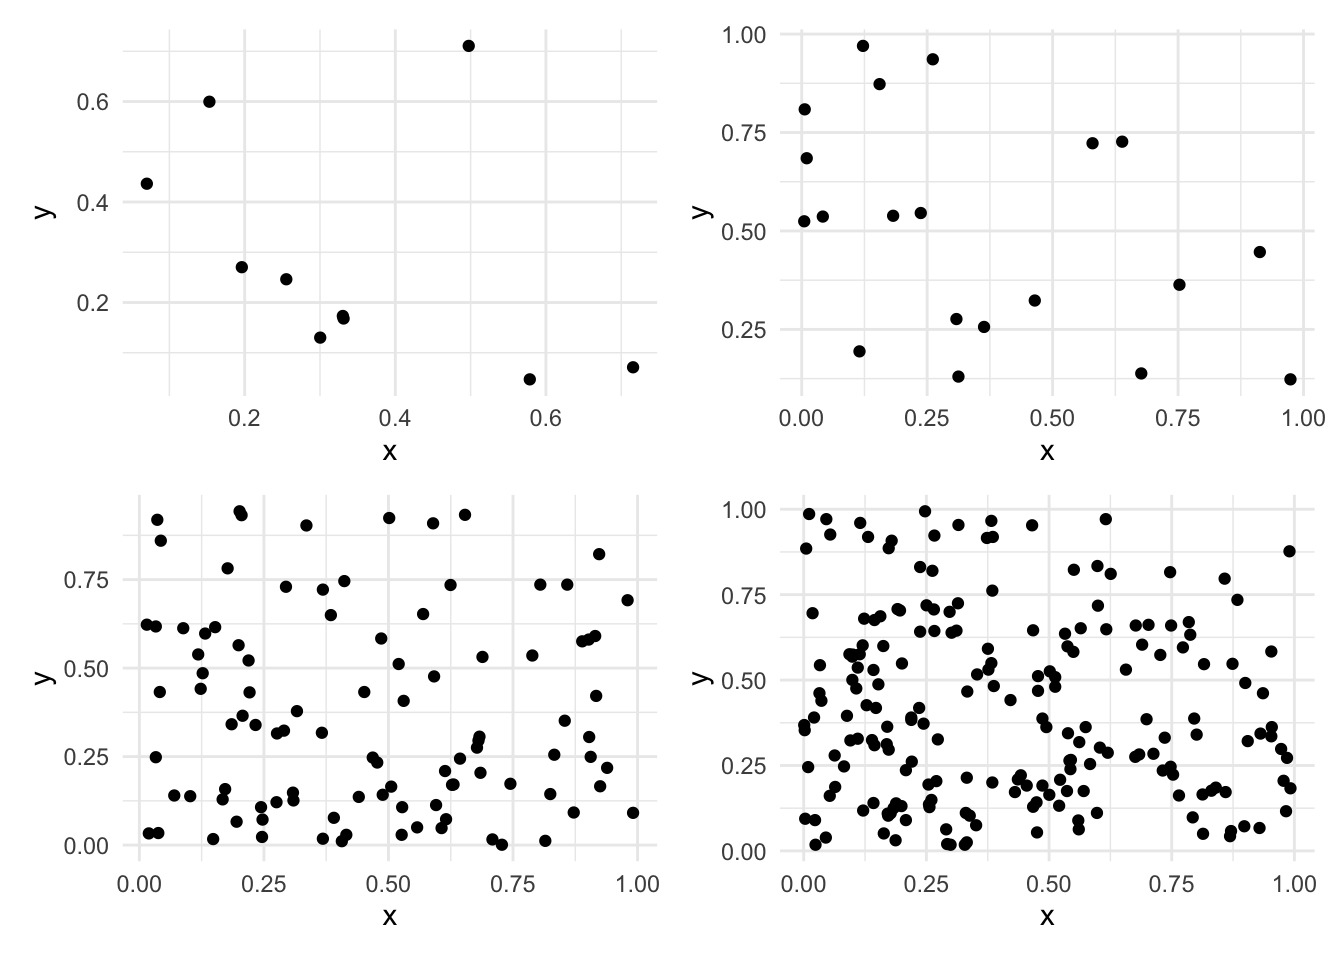
\includegraphics{08-regression-estimation_files/figure-pdf/create plots of sampled data-1.pdf}

\begin{Shaded}
\begin{Highlighting}[]
\NormalTok{model\_10    }\OtherTok{\textless{}{-}} \FunctionTok{lm}\NormalTok{(y }\SpecialCharTok{\textasciitilde{}}\NormalTok{ x, }\AttributeTok{data =}\NormalTok{ sample\_10)}
\NormalTok{model\_100   }\OtherTok{\textless{}{-}} \FunctionTok{lm}\NormalTok{(y }\SpecialCharTok{\textasciitilde{}}\NormalTok{ x, }\AttributeTok{data =}\NormalTok{ sample\_100)}
\NormalTok{model\_200   }\OtherTok{\textless{}{-}} \FunctionTok{lm}\NormalTok{(y }\SpecialCharTok{\textasciitilde{}}\NormalTok{ x, }\AttributeTok{data =}\NormalTok{ sample\_200)}
\NormalTok{model\_10000 }\OtherTok{\textless{}{-}} \FunctionTok{lm}\NormalTok{(y }\SpecialCharTok{\textasciitilde{}}\NormalTok{ x, }\AttributeTok{data =}\NormalTok{ sample\_10000)}

\FunctionTok{coef}\NormalTok{(model\_10)}
\end{Highlighting}
\end{Shaded}

\begin{verbatim}
(Intercept)           x 
  0.5712492  -0.6584944 
\end{verbatim}

\begin{Shaded}
\begin{Highlighting}[]
\NormalTok{results\_10 }\OtherTok{\textless{}{-}} \ConstantTok{NA} 
\ControlFlowTok{for}\NormalTok{(i }\ControlFlowTok{in} \DecValTok{1}\SpecialCharTok{:}\DecValTok{100}\NormalTok{) \{ }
\NormalTok{  sample\_10  }\OtherTok{\textless{}{-}}\NormalTok{ d }\SpecialCharTok{|\textgreater{}} \FunctionTok{slice\_sample}\NormalTok{(}\AttributeTok{n =} \DecValTok{10}\NormalTok{, }\AttributeTok{weight\_by =}\NormalTok{ prob)}
\NormalTok{  model\_10   }\OtherTok{\textless{}{-}} \FunctionTok{lm}\NormalTok{(y }\SpecialCharTok{\textasciitilde{}}\NormalTok{ x, }\AttributeTok{data =}\NormalTok{ sample\_10)}
\NormalTok{  results\_10[i] }\OtherTok{\textless{}{-}} \FunctionTok{coef}\NormalTok{(model\_10)[}\StringTok{\textquotesingle{}x\textquotesingle{}}\NormalTok{]}
\NormalTok{\}}

\NormalTok{results\_200 }\OtherTok{\textless{}{-}} \ConstantTok{NA} 
\ControlFlowTok{for}\NormalTok{(i }\ControlFlowTok{in} \DecValTok{1}\SpecialCharTok{:}\DecValTok{100}\NormalTok{) \{ }
\NormalTok{  sample\_200  }\OtherTok{\textless{}{-}}\NormalTok{ d }\SpecialCharTok{|\textgreater{}} \FunctionTok{slice\_sample}\NormalTok{(}\AttributeTok{n =} \DecValTok{200}\NormalTok{, }\AttributeTok{weight\_by =}\NormalTok{ prob)}
\NormalTok{  model\_200   }\OtherTok{\textless{}{-}} \FunctionTok{lm}\NormalTok{(y }\SpecialCharTok{\textasciitilde{}}\NormalTok{ x, }\AttributeTok{data =}\NormalTok{ sample\_200)}
\NormalTok{  results\_200[i] }\OtherTok{\textless{}{-}} \FunctionTok{coef}\NormalTok{(model\_200)[}\StringTok{\textquotesingle{}x\textquotesingle{}}\NormalTok{]}
\NormalTok{  \}}
\end{Highlighting}
\end{Shaded}

\begin{Shaded}
\begin{Highlighting}[]
\NormalTok{plot\_10 }\OtherTok{\textless{}{-}} \FunctionTok{ggplot}\NormalTok{() }\SpecialCharTok{+} 
  \FunctionTok{aes}\NormalTok{(}\AttributeTok{x=}\NormalTok{results\_10) }\SpecialCharTok{+} 
  \FunctionTok{geom\_histogram}\NormalTok{()}

\NormalTok{plot\_200 }\OtherTok{\textless{}{-}} \FunctionTok{ggplot}\NormalTok{() }\SpecialCharTok{+} 
  \FunctionTok{aes}\NormalTok{(}\AttributeTok{x=}\NormalTok{results\_200) }\SpecialCharTok{+} 
  \FunctionTok{geom\_histogram}\NormalTok{()}
  
\NormalTok{plot\_10 }\SpecialCharTok{/} 
\NormalTok{  plot\_200}
\end{Highlighting}
\end{Shaded}

\begin{verbatim}
`stat_bin()` using `bins = 30`. Pick better value with `binwidth`.
`stat_bin()` using `bins = 30`. Pick better value with `binwidth`.
\end{verbatim}

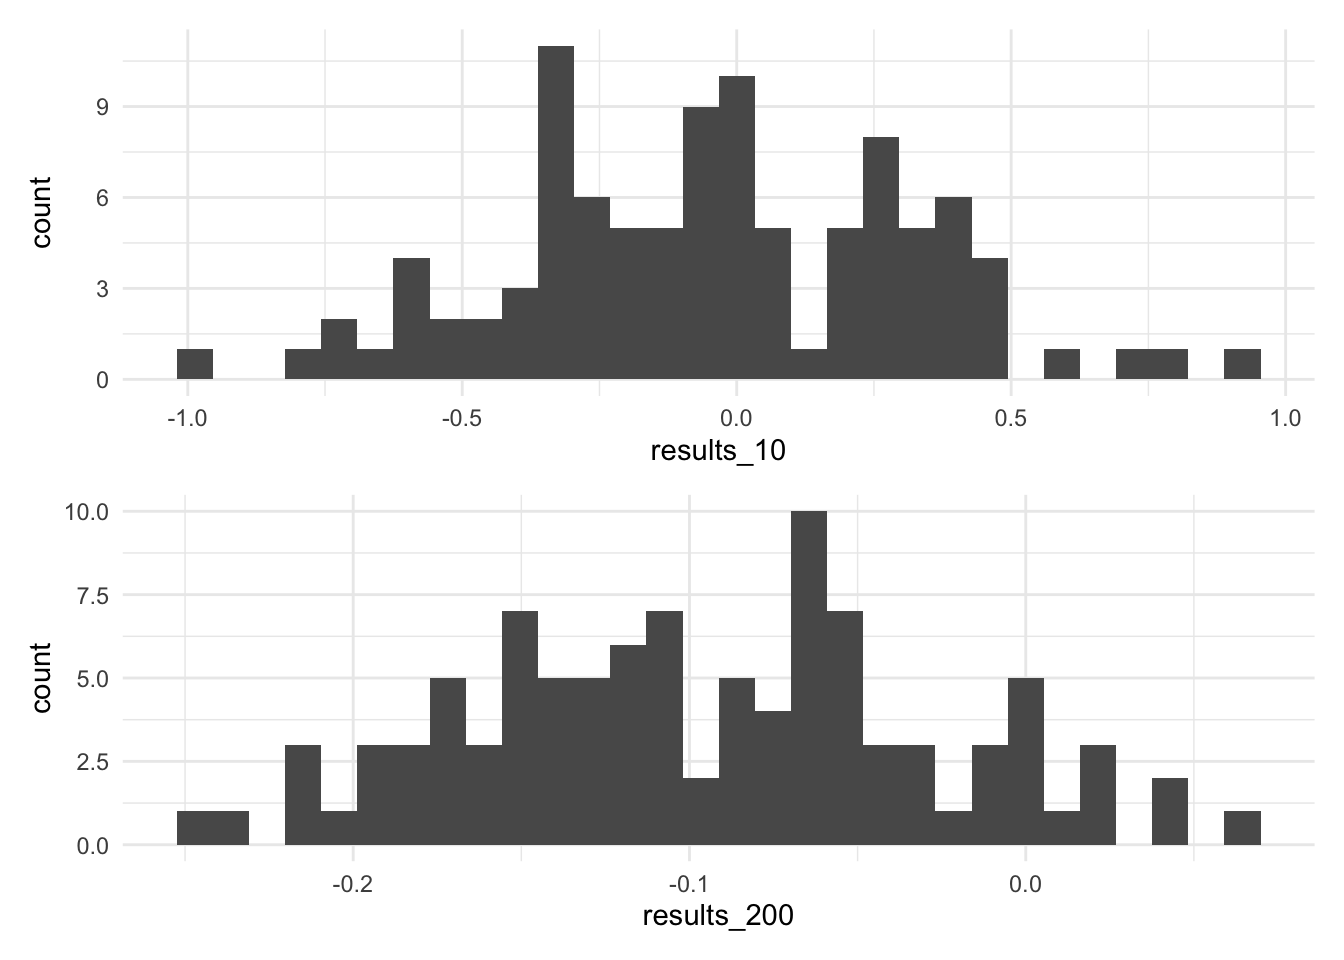
\includegraphics{08-regression-estimation_files/figure-pdf/simulations of coefficients 2-1.pdf}

\section{The Regression Anatomy
Formula}\label{the-regression-anatomy-formula}

We make the claim in live session that we can re-represent a coefficient
that we're interested in as a function of all the other variable in a
regression. That is, suppose that we were interested, initially, in
estimating the model:

\[ 
Y = \hat\beta_{0} + \hat\beta_{1} X_{1} + \hat\beta_{2} X_{2} + \hat\beta_{3}X_{3} + e
\] that we can produce an estimate for \(\hat\beta_{1}\) by fitting this
auxiliary regression,

\[
X_{1} = \hat\delta_{0} + \hat\delta_2X_2 + \hat\delta_3X_3 + r_{1}
\]

And then using the residuals, noted as \(r_1\) above, in a second
auxiliary regression,

\[ 
Y = \gamma_0 + \gamma_1 r_1
\]

The claim that we make in the live session is that there is a guarantee
that \(\beta_1 = \gamma_1\). Here, we are first going to show that this
is true, and then we're going to reason about what this means, and why
this feature is interesting (or at least useful) when we are estimating
a regression.

Suppose that the population model is the following:

\[
X_{1} = 
\begin{cases}
  \frac{1}{10}, & 0 \leq x \leq 10, \\ 
  0, & otherwise
\end{cases}
\]

\[
X_{2} = 
\begin{cases}
  \frac{1}{10}, & 0 \leq x \leq 10, \\ 
  0, & otherwise
\end{cases}
\]

\[
X_{3} = 
\begin{cases}
  \frac{1}{10}, & 0 \leq x \leq 10, \\ 
  0, & otherwise
\end{cases}
\] And, furthermore suppose that \(Y = g(X_{1}, X_{2}, X_{3}\),
specifically, that:

\[
Y = -3 + (1\cdot X_1) + (2\cdot X_2) + (3\cdot X_3)
\] Then, because we know the population model, we can produce a single
sample from it using the following code:

\begin{Shaded}
\begin{Highlighting}[]
\NormalTok{d }\OtherTok{\textless{}{-}} \FunctionTok{data.frame}\NormalTok{(}
  \AttributeTok{x1 =} \FunctionTok{runif}\NormalTok{(}\AttributeTok{n =} \DecValTok{100}\NormalTok{, }\AttributeTok{min =} \DecValTok{0}\NormalTok{, }\AttributeTok{max =} \DecValTok{10}\NormalTok{), }
  \AttributeTok{x2 =} \FunctionTok{runif}\NormalTok{(}\AttributeTok{n =} \DecValTok{100}\NormalTok{, }\AttributeTok{min =} \DecValTok{0}\NormalTok{, }\AttributeTok{max =} \DecValTok{10}\NormalTok{), }
  \AttributeTok{x3 =} \FunctionTok{runif}\NormalTok{(}\AttributeTok{n =} \DecValTok{100}\NormalTok{, }\AttributeTok{min =} \DecValTok{0}\NormalTok{, }\AttributeTok{max =} \DecValTok{10}\NormalTok{)) }\SpecialCharTok{\%\textgreater{}\%} 
  \FunctionTok{mutate}\NormalTok{(}\AttributeTok{y =} \SpecialCharTok{{-}}\DecValTok{3} \SpecialCharTok{+} \DecValTok{1}\SpecialCharTok{*}\NormalTok{x1 }\SpecialCharTok{+} \DecValTok{2}\SpecialCharTok{*}\NormalTok{x2 }\SpecialCharTok{+} \DecValTok{3}\SpecialCharTok{*}\NormalTok{x3 }\SpecialCharTok{+} \FunctionTok{rnorm}\NormalTok{(}\AttributeTok{n =} \FunctionTok{n}\NormalTok{(), }\AttributeTok{mean =} \DecValTok{0}\NormalTok{, }\AttributeTok{sd =} \DecValTok{1}\NormalTok{))}

\FunctionTok{head}\NormalTok{(d)}
\end{Highlighting}
\end{Shaded}

\begin{verbatim}
         x1       x2       x3        y
1 3.9705884 1.872222 5.707056 22.52463
2 3.2725536 3.059597 9.289013 32.68092
3 2.3639867 5.095805 3.103407 19.69738
4 1.9705959 4.849187 6.205846 26.85517
5 3.4629530 4.088009 8.369140 34.72584
6 0.2704242 5.695944 5.543990 25.42245
\end{verbatim}

Notice that when we made this data, we included a set of random noise at
the end. The idea here is that there are other ``things'' in this
universe that also affect \(Y\), but that we don't have access to them.
By assumption, what we \emph{have} measured in this world,
\(X_1, X_2, X_3\) are uncorrelated with these other features.

\subsection{Estimate an OLS
Regression}\label{estimate-an-ols-regression}

Let's begin by producing an estimate of the OLS regression of Y on these
X variables. Notice the way that we're talking about this:

\begin{quote}
We are going to regress Y on \(X_{1}\), \(X_{2}\), and \(X_{3}\).
\end{quote}

\begin{Shaded}
\begin{Highlighting}[]
\NormalTok{model\_main }\OtherTok{\textless{}{-}} \FunctionTok{lm}\NormalTok{(y }\SpecialCharTok{\textasciitilde{}}\NormalTok{ x1 }\SpecialCharTok{+}\NormalTok{ x2 }\SpecialCharTok{+}\NormalTok{ x3, }\AttributeTok{data =}\NormalTok{ d)}
\FunctionTok{coef}\NormalTok{(model\_main)}
\end{Highlighting}
\end{Shaded}

\begin{verbatim}
(Intercept)          x1          x2          x3 
  -2.992210    1.064760    2.002090    2.948275 
\end{verbatim}

\subsection{Regression Anatomy and Fritch Waugh
Lovell}\label{regression-anatomy-and-fritch-waugh-lovell}

The claim is that we can produce an estimate of \(\hat{\beta}_1\) using
an auxiliary set of regression estimates, and then using the regression
from that auxiliary regression.

\begin{Shaded}
\begin{Highlighting}[]
\NormalTok{model\_aux }\OtherTok{\textless{}{-}} \FunctionTok{lm}\NormalTok{(x1 }\SpecialCharTok{\textasciitilde{}}\NormalTok{ x2 }\SpecialCharTok{+}\NormalTok{ x3, }\AttributeTok{data =}\NormalTok{ d)}
\end{Highlighting}
\end{Shaded}

If we look into the structure of \texttt{model\_aux} we can see that
there are \emph{a ton} of pieces in here.

\begin{Shaded}
\begin{Highlighting}[]
\FunctionTok{str}\NormalTok{(model\_aux)}
\end{Highlighting}
\end{Shaded}

\begin{verbatim}
List of 12
 $ coefficients : Named num [1:3] 5.13916 -0.1211 0.00813
  ..- attr(*, "names")= chr [1:3] "(Intercept)" "x2" "x3"
 $ residuals    : Named num [1:100] -0.988 -1.572 -2.183 -2.632 -1.249 ...
  ..- attr(*, "names")= chr [1:100] "1" "2" "3" "4" ...
 $ effects      : Named num [1:100] -45.966 -3.398 0.224 -2.638 -1.37 ...
  ..- attr(*, "names")= chr [1:100] "(Intercept)" "x2" "x3" "" ...
 $ rank         : int 3
 $ fitted.values: Named num [1:100] 4.96 4.84 4.55 4.6 4.71 ...
  ..- attr(*, "names")= chr [1:100] "1" "2" "3" "4" ...
 $ assign       : int [1:3] 0 1 2
 $ qr           :List of 5
  ..$ qr   : num [1:100, 1:3] -10 0.1 0.1 0.1 0.1 0.1 0.1 0.1 0.1 0.1 ...
  .. ..- attr(*, "dimnames")=List of 2
  .. .. ..$ : chr [1:100] "1" "2" "3" "4" ...
  .. .. ..$ : chr [1:3] "(Intercept)" "x2" "x3"
  .. ..- attr(*, "assign")= int [1:3] 0 1 2
  ..$ qraux: num [1:3] 1.1 1.05 1.07
  ..$ pivot: int [1:3] 1 2 3
  ..$ tol  : num 1e-07
  ..$ rank : int 3
  ..- attr(*, "class")= chr "qr"
 $ df.residual  : int 97
 $ xlevels      : Named list()
 $ call         : language lm(formula = x1 ~ x2 + x3, data = d)
 $ terms        :Classes 'terms', 'formula'  language x1 ~ x2 + x3
  .. ..- attr(*, "variables")= language list(x1, x2, x3)
  .. ..- attr(*, "factors")= int [1:3, 1:2] 0 1 0 0 0 1
  .. .. ..- attr(*, "dimnames")=List of 2
  .. .. .. ..$ : chr [1:3] "x1" "x2" "x3"
  .. .. .. ..$ : chr [1:2] "x2" "x3"
  .. ..- attr(*, "term.labels")= chr [1:2] "x2" "x3"
  .. ..- attr(*, "order")= int [1:2] 1 1
  .. ..- attr(*, "intercept")= int 1
  .. ..- attr(*, "response")= int 1
  .. ..- attr(*, ".Environment")=<environment: R_GlobalEnv> 
  .. ..- attr(*, "predvars")= language list(x1, x2, x3)
  .. ..- attr(*, "dataClasses")= Named chr [1:3] "numeric" "numeric" "numeric"
  .. .. ..- attr(*, "names")= chr [1:3] "x1" "x2" "x3"
 $ model        :'data.frame':  100 obs. of  3 variables:
  ..$ x1: num [1:100] 3.97 3.27 2.36 1.97 3.46 ...
  ..$ x2: num [1:100] 1.87 3.06 5.1 4.85 4.09 ...
  ..$ x3: num [1:100] 5.71 9.29 3.1 6.21 8.37 ...
  ..- attr(*, "terms")=Classes 'terms', 'formula'  language x1 ~ x2 + x3
  .. .. ..- attr(*, "variables")= language list(x1, x2, x3)
  .. .. ..- attr(*, "factors")= int [1:3, 1:2] 0 1 0 0 0 1
  .. .. .. ..- attr(*, "dimnames")=List of 2
  .. .. .. .. ..$ : chr [1:3] "x1" "x2" "x3"
  .. .. .. .. ..$ : chr [1:2] "x2" "x3"
  .. .. ..- attr(*, "term.labels")= chr [1:2] "x2" "x3"
  .. .. ..- attr(*, "order")= int [1:2] 1 1
  .. .. ..- attr(*, "intercept")= int 1
  .. .. ..- attr(*, "response")= int 1
  .. .. ..- attr(*, ".Environment")=<environment: R_GlobalEnv> 
  .. .. ..- attr(*, "predvars")= language list(x1, x2, x3)
  .. .. ..- attr(*, "dataClasses")= Named chr [1:3] "numeric" "numeric" "numeric"
  .. .. .. ..- attr(*, "names")= chr [1:3] "x1" "x2" "x3"
 - attr(*, "class")= chr "lm"
\end{verbatim}

To evaluate our claim, we need to find the residuals from this
regression. As a knowledge check, what is it that we mean when we say,
``residual'' in this sense?

To make talking about these easier, here is a plot that might be useful.

\begin{Shaded}
\begin{Highlighting}[]
\NormalTok{d }\SpecialCharTok{\%\textgreater{}\%} 
  \FunctionTok{ggplot}\NormalTok{() }\SpecialCharTok{+} 
  \FunctionTok{aes}\NormalTok{(}\AttributeTok{x =}\NormalTok{ x1, }\AttributeTok{y =}\NormalTok{ y) }\SpecialCharTok{+} 
  \FunctionTok{geom\_point}\NormalTok{() }\SpecialCharTok{+} 
  \FunctionTok{geom\_segment}\NormalTok{(}\FunctionTok{aes}\NormalTok{(}\AttributeTok{x =} \DecValTok{0}\NormalTok{, }\AttributeTok{xend =} \DecValTok{10}\NormalTok{, }\AttributeTok{y =} \DecValTok{0}\NormalTok{, }\AttributeTok{yend =} \DecValTok{50}\NormalTok{), }\AttributeTok{color =} \StringTok{\textquotesingle{}steelblue\textquotesingle{}}\NormalTok{)}
\end{Highlighting}
\end{Shaded}

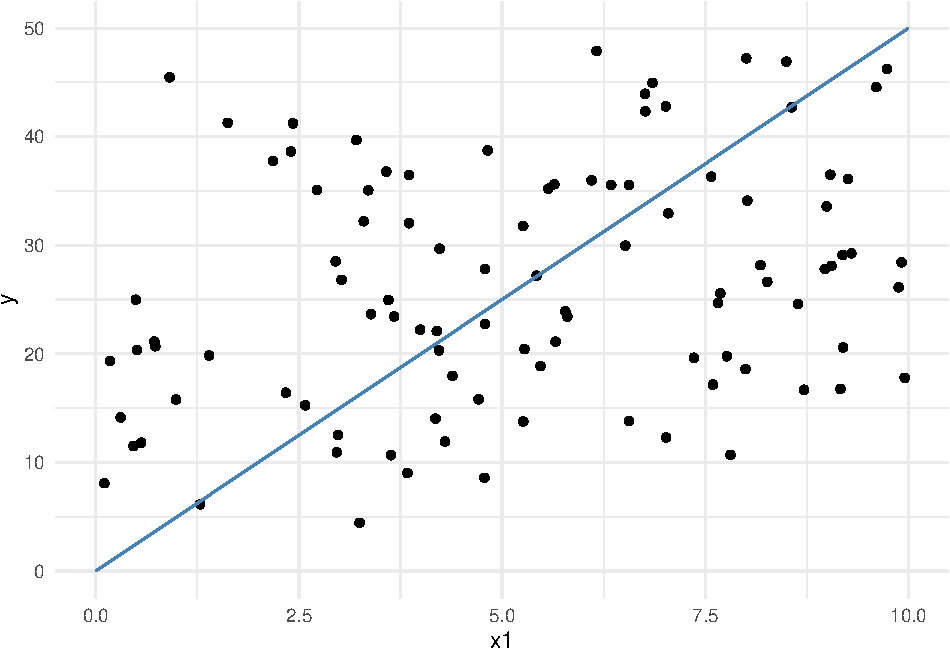
\includegraphics{08-regression-estimation_files/figure-pdf/plot x1 and y and line-1.pdf}

In order to access these residuals, we can ``augment'' the dataframe
that we used in the model, using the \texttt{broom::augment} function
call.

\begin{Shaded}
\begin{Highlighting}[]
\NormalTok{model\_aux\_augmented }\OtherTok{\textless{}{-}} \FunctionTok{augment}\NormalTok{(model\_aux)}
\end{Highlighting}
\end{Shaded}

Because the \(Y\) variable wasn't included in the regression for
\texttt{model\_aux} we have to bring of over from the main dataset,
which is a little bit\ldots{} um, hacky. Forgive these sins.

\begin{Shaded}
\begin{Highlighting}[]
\NormalTok{model\_aux\_augmented}\SpecialCharTok{$}\NormalTok{y }\OtherTok{\textless{}{-}}\NormalTok{ d}\SpecialCharTok{$}\NormalTok{y}
\NormalTok{model\_aux\_augmented}
\end{Highlighting}
\end{Shaded}

\begin{verbatim}
# A tibble: 100 x 10
       x1    x2    x3 .fitted .resid   .hat .sigma  .cooksd .std.resid     y
    <dbl> <dbl> <dbl>   <dbl>  <dbl>  <dbl>  <dbl>    <dbl>      <dbl> <dbl>
 1 3.97    1.87 5.71     4.96 -0.988 0.0221   2.93 0.000885     -0.342 22.5 
 2 3.27    3.06 9.29     4.84 -1.57  0.0399   2.93 0.00418      -0.549 32.7 
 3 2.36    5.10 3.10     4.55 -2.18  0.0151   2.93 0.00291      -0.754 19.7 
 4 1.97    4.85 6.21     4.60 -2.63  0.0118   2.92 0.00328      -0.907 26.9 
 5 3.46    4.09 8.37     4.71 -1.25  0.0260   2.93 0.00167      -0.434 34.7 
 6 0.270   5.70 5.54     4.49 -4.22  0.0112   2.90 0.00799      -1.46  25.4 
 7 0.251   9.61 5.45     4.02 -3.77  0.0387   2.91 0.0233       -1.32  33.5 
 8 2.63    1.02 0.918    5.02 -2.39  0.0462   2.92 0.0114       -0.839  3.62
 9 8.80    7.75 7.29     4.26  4.54  0.0258   2.90 0.0219        1.58  43.4 
10 0.0256  5.17 3.72     4.54 -4.52  0.0125   2.90 0.0103       -1.56  18.7 
# i 90 more rows
\end{verbatim}

Finally, with this augmented data that has information from the model,
we can estimate the model that includes only the residuals as predictors
of \(Y\).

\begin{Shaded}
\begin{Highlighting}[]
\NormalTok{model\_two }\OtherTok{\textless{}{-}} \FunctionTok{lm}\NormalTok{(y }\SpecialCharTok{\textasciitilde{}}\NormalTok{ .resid, }\AttributeTok{data =}\NormalTok{ model\_aux\_augmented)}
\FunctionTok{coef}\NormalTok{(model\_two)}
\end{Highlighting}
\end{Shaded}

\begin{verbatim}
(Intercept)      .resid 
   26.38423     1.06476 
\end{verbatim}

Our claim was that the coefficients from \texttt{model\_main} and
\texttt{model\_two} should be the same.

\begin{Shaded}
\begin{Highlighting}[]
\FunctionTok{test\_that}\NormalTok{(}
  \StringTok{\textquotesingle{}the model coefficients are equal\textquotesingle{}}\NormalTok{, }
  \FunctionTok{expect\_equal}\NormalTok{(}
    \FunctionTok{as.numeric}\NormalTok{(}\FunctionTok{coef}\NormalTok{(model\_main)[}\StringTok{\textquotesingle{}x1\textquotesingle{}}\NormalTok{]), }
    \FunctionTok{as.numeric}\NormalTok{(}\FunctionTok{coef}\NormalTok{(model\_two)[}\StringTok{\textquotesingle{}.resid\textquotesingle{}}\NormalTok{]))}
\NormalTok{)}
\end{Highlighting}
\end{Shaded}

\begin{verbatim}
Test passed 
\end{verbatim}

But, why is this an interesting, or at least useful, feature to
appreciate?

This is actually a really famous, relatively recently ``rediscovered''
proof. If we have a number of variables, one called an outcome and the
rest called features, then we can estimate the relationship between the
outcome and one feature in the following way:

\begin{enumerate}
\def\labelenumi{\arabic{enumi}.}
\tightlist
\item
  Estimate the relationship between all the other features and the one
  that we're examining; save the information about the feature we're
  examining which cannot be explained by the other features in some
  vector.
\item
  Regress the outcome on this leftover information.
\end{enumerate}

Slightly more of what is happening? In the first model, the leftover
information is orthogonal to the information posessed in the regression
features. In the second model, we can use this orthagonal information to
estimate the effect of one variable.

\section{Coding Activity:R Cheat
Sheet}\label{coding-activityr-cheat-sheet}

Suppose \texttt{x} and \texttt{y} are variables in dataframe \texttt{d}.

To fit an ols regression of Y on X:

\begin{verbatim}
mod <- lm(y ~ x, data = d)
\end{verbatim}

To access \textbf{coefficients} from the model object:

\begin{verbatim}
mod$coefficients
or coef(mod)
\end{verbatim}

To access \textbf{fitted values} from the model object:

\begin{verbatim}
mod$fitted
or fitted(mod)
or predict(mod)
\end{verbatim}

To access \textbf{residuals} from the model object:

\begin{verbatim}
mod$residuals
or resid(mod)
\end{verbatim}

To create a scatterplot that includes the regression line:

\begin{verbatim}
plot(d['x'], d['y'])
abline(mod)
or 
d %>% 
  ggplot() + 
  aes(x = x, y = y) + 
  geom_point() + 
  geom_smooth(method = lm)
\end{verbatim}

\section{R Exercise}\label{r-exercise}

\textbf{Real Estate in Boston}

The file \texttt{hprice1.Rdata} contains 88 observations of homes in the
Boston area, taken from the real estate pages of the Boston Globe during
1990. This data was provided by Wooldridge.

\begin{Shaded}
\begin{Highlighting}[]
\FunctionTok{load}\NormalTok{(}\StringTok{\textquotesingle{}data/hprice1.RData\textquotesingle{}}\NormalTok{) }\CommentTok{\# provides 3 objects }
\end{Highlighting}
\end{Shaded}

\begin{Shaded}
\begin{Highlighting}[]
\FunctionTok{head}\NormalTok{(data)}
\end{Highlighting}
\end{Shaded}

\begin{verbatim}
    price assess bdrms lotsize sqrft colonial   lprice  lassess llotsize
1 300.000  349.1     4    6126  2438        1 5.703783 5.855359 8.720297
2 370.000  351.5     3    9903  2076        1 5.913503 5.862210 9.200593
3 191.000  217.7     3    5200  1374        0 5.252274 5.383118 8.556414
4 195.000  231.8     3    4600  1448        1 5.273000 5.445875 8.433811
5 373.000  319.1     4    6095  2514        1 5.921578 5.765504 8.715224
6 466.275  414.5     5    8566  2754        1 6.144775 6.027073 9.055556
    lsqrft
1 7.798934
2 7.638198
3 7.225482
4 7.277938
5 7.829630
6 7.920810
\end{verbatim}

\begin{itemize}
\tightlist
\item
  Are there variables that would \emph{not} be valid outcomes for an OLS
  regression? If so, why?
\item
  Are there variables that would \emph{not} be valid inputs for an OLS
  regression? If so, why?
\end{itemize}

\subsection{Assess the Relationship between Price and Square
Footage}\label{assess-the-relationship-between-price-and-square-footage}

\begin{Shaded}
\begin{Highlighting}[]
\NormalTok{data }\SpecialCharTok{\%\textgreater{}\%} 
  \FunctionTok{ggplot}\NormalTok{() }\SpecialCharTok{+} 
  \FunctionTok{aes}\NormalTok{(}\AttributeTok{x=}\NormalTok{sqrft, }\AttributeTok{y=}\NormalTok{price) }\SpecialCharTok{+} 
  \FunctionTok{geom\_point}\NormalTok{()}
\end{Highlighting}
\end{Shaded}

\includegraphics{08-regression-estimation_files/figure-pdf/unnamed-chunk-8-1.pdf}

Suppose that you're interested in knowing the relationship between price
and square footage.

\begin{enumerate}
\def\labelenumi{\arabic{enumi}.}
\setcounter{enumi}{-1}
\item
  Assess the assumptions of the Large-Sample Linear Model.
\item
  Create a scatterplot of \texttt{price} and \texttt{sqrft}. Like every
  plot you make, ensure that the plot \emph{minimally} has a title and
  meaningful axes.
\end{enumerate}

\begin{enumerate}
\def\labelenumi{\arabic{enumi}.}
\setcounter{enumi}{1}
\item
  Find the correlation between the two variables.
\item
  Recall the equation for the slope of the OLS regression line -- here
  you can either use Variance and Covariance, or if you're bold, the
  linear algebra. Compute the slope manually (without using
  \texttt{lm()})
\end{enumerate}

\begin{enumerate}
\def\labelenumi{\arabic{enumi}.}
\setcounter{enumi}{3}
\tightlist
\item
  Regress \texttt{price} on \texttt{sqrft} using the \texttt{lm}
  function. This will produce an estimate for the following model:
\end{enumerate}

{[} price = \beta\emph{\{0\} + \beta}\{1\} sqrft + e {]}

\begin{Shaded}
\begin{Highlighting}[]
\NormalTok{data }\SpecialCharTok{\%\textgreater{}\%} 
  \FunctionTok{ggplot}\NormalTok{() }\SpecialCharTok{+} 
  \FunctionTok{aes}\NormalTok{(}\AttributeTok{x=}\NormalTok{sqrft, }\AttributeTok{y=}\NormalTok{lotsize) }\SpecialCharTok{+} 
  \FunctionTok{geom\_point}\NormalTok{()}
\end{Highlighting}
\end{Shaded}

\includegraphics{08-regression-estimation_files/figure-pdf/unnamed-chunk-12-1.pdf}

\begin{enumerate}
\def\labelenumi{\arabic{enumi}.}
\setcounter{enumi}{4}
\tightlist
\item
  Create a scatterplot that includes the fitted regression.
\end{enumerate}

\begin{enumerate}
\def\labelenumi{\arabic{enumi}.}
\setcounter{enumi}{5}
\tightlist
\item
  Interpret what the coefficient means.
\end{enumerate}

\begin{itemize}
\tightlist
\item
  State what features you are allowing to change and what features
  you're requiring do not change.
\item
  For each additional square foot, how much more (or less) is the house
  worth?
\end{itemize}

\begin{enumerate}
\def\labelenumi{\arabic{enumi}.}
\setcounter{enumi}{6}
\tightlist
\item
  Estimate a new model (and save it into another object) that includes
  the size of the lot and whether the house is a colonial. This will
  estimate the model:
\end{enumerate}

\[
price = \beta_{0} + \beta_{1} sqrft + \beta_{2} lotsize + \beta_{3} colonial? + e
\]

\begin{itemize}
\tightlist
\item
  \emph{BUT BEFORE YOU DO}, make a prediction: What do you think is
  going to happen to the coefficient that relates square footage and
  price?

  \begin{itemize}
  \tightlist
  \item
    Will the coefficient increase, decrease, or stay the same?
  \end{itemize}
\end{itemize}

\begin{enumerate}
\def\labelenumi{\arabic{enumi}.}
\setcounter{enumi}{6}
\tightlist
\item
  Compute the sample correlation between \(X\) and \(e_i\). What
  guarantees do we have from the book about this correlation? Does the
  data seem to bear this out?
\end{enumerate}

\section{Regression Plots and
Discussion}\label{regression-plots-and-discussion}

In this next set of notes, we're going to give some data, displayed in
plots, and we will try to apply what we have learned in the async and
reading for this week to answer questions about each of the scatter
plots.

\subsection{Plot 1}\label{plot-1}

Consider data that is generated according to the following function:

\[
  Y = 1 + 2x_1 + 3x_2 + e, 
\]

where \(x_1 \sim N(0,2)\), \(x_2 \sim N(0,2)\) and \(e\) is a constant
equal to zero.

From this population, you might consider taking a sample of 100
observations, and representing this data in the following 3d scatter
plot. In this plot, there are three dimensions, an \(x_1, x_2\), and
\(y\) dimensions.

\begin{Shaded}
\begin{Highlighting}[]
\NormalTok{knitr}\SpecialCharTok{::}\FunctionTok{include\_app}\NormalTok{(}\AttributeTok{url =}\StringTok{"http://www.statistics.wtf/minibeta01/"}\NormalTok{)}
\end{Highlighting}
\end{Shaded}

\href{http://www.statistics.wtf/minibeta01/}{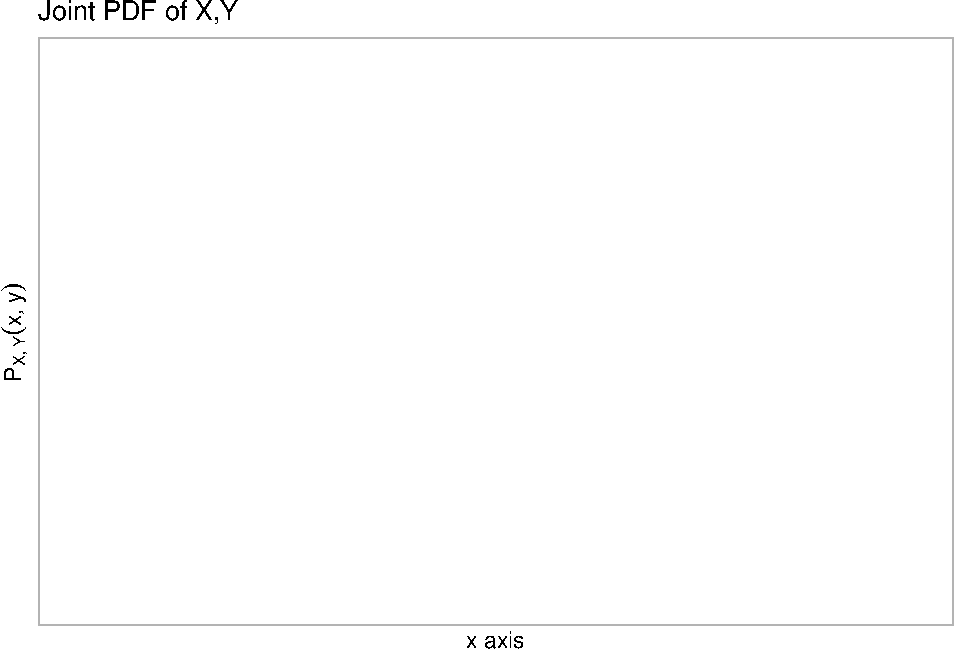
\includegraphics{08-regression-estimation_files/figure-pdf/unnamed-chunk-15-1.pdf}}

\begin{enumerate}
\def\labelenumi{\arabic{enumi}.}
\tightlist
\item
  Rotate the cube and explore the data, looking at each face of the
  cube, including from the top down.
\item
  One of the lessons that we learned during the random variables section
  of the course is that every random variable that has been measured can
  also be marginalized off. You might think of this as ``casting down''
  data from three dimensions, to only two.
\item
  Sketch the following 2d scatter plots, taking care the label your
  axes. You need not represent all 100 points, but rather create the
  \emph{gestalt} of what you see.\\
  1. \(Y = f(x_1)\) (but not \(x_2\)) 2. \(Y = f(x_2)\) (but not
  \(x_1\)) 3. \(x2 = f(x_1)\)
\item
  Once you have sketched the scatter plots, what line would you fit that
  minimizes the sum of squared residuals in the vertical direction.
  Define a residual, \(\epsilon\), to be the vertical distance between
  the line you draw, and the corresponding point on the input data.
\item
  What is the \emph{average} of the residuals for each of the lines that
  you have fitted? How does this correspond to the \emph{moment
  conditions} discussed in the async? What would happen if you
  translated this line vertically?
\item
  Rotate the cube so that the points ``fall into line''. When you see
  this line, how does it help you describe the function that governs
  this data?
\end{enumerate}

\chapter{OLS Regression Inference}\label{ols-regression-inference}

\begin{figure}[H]

{\centering 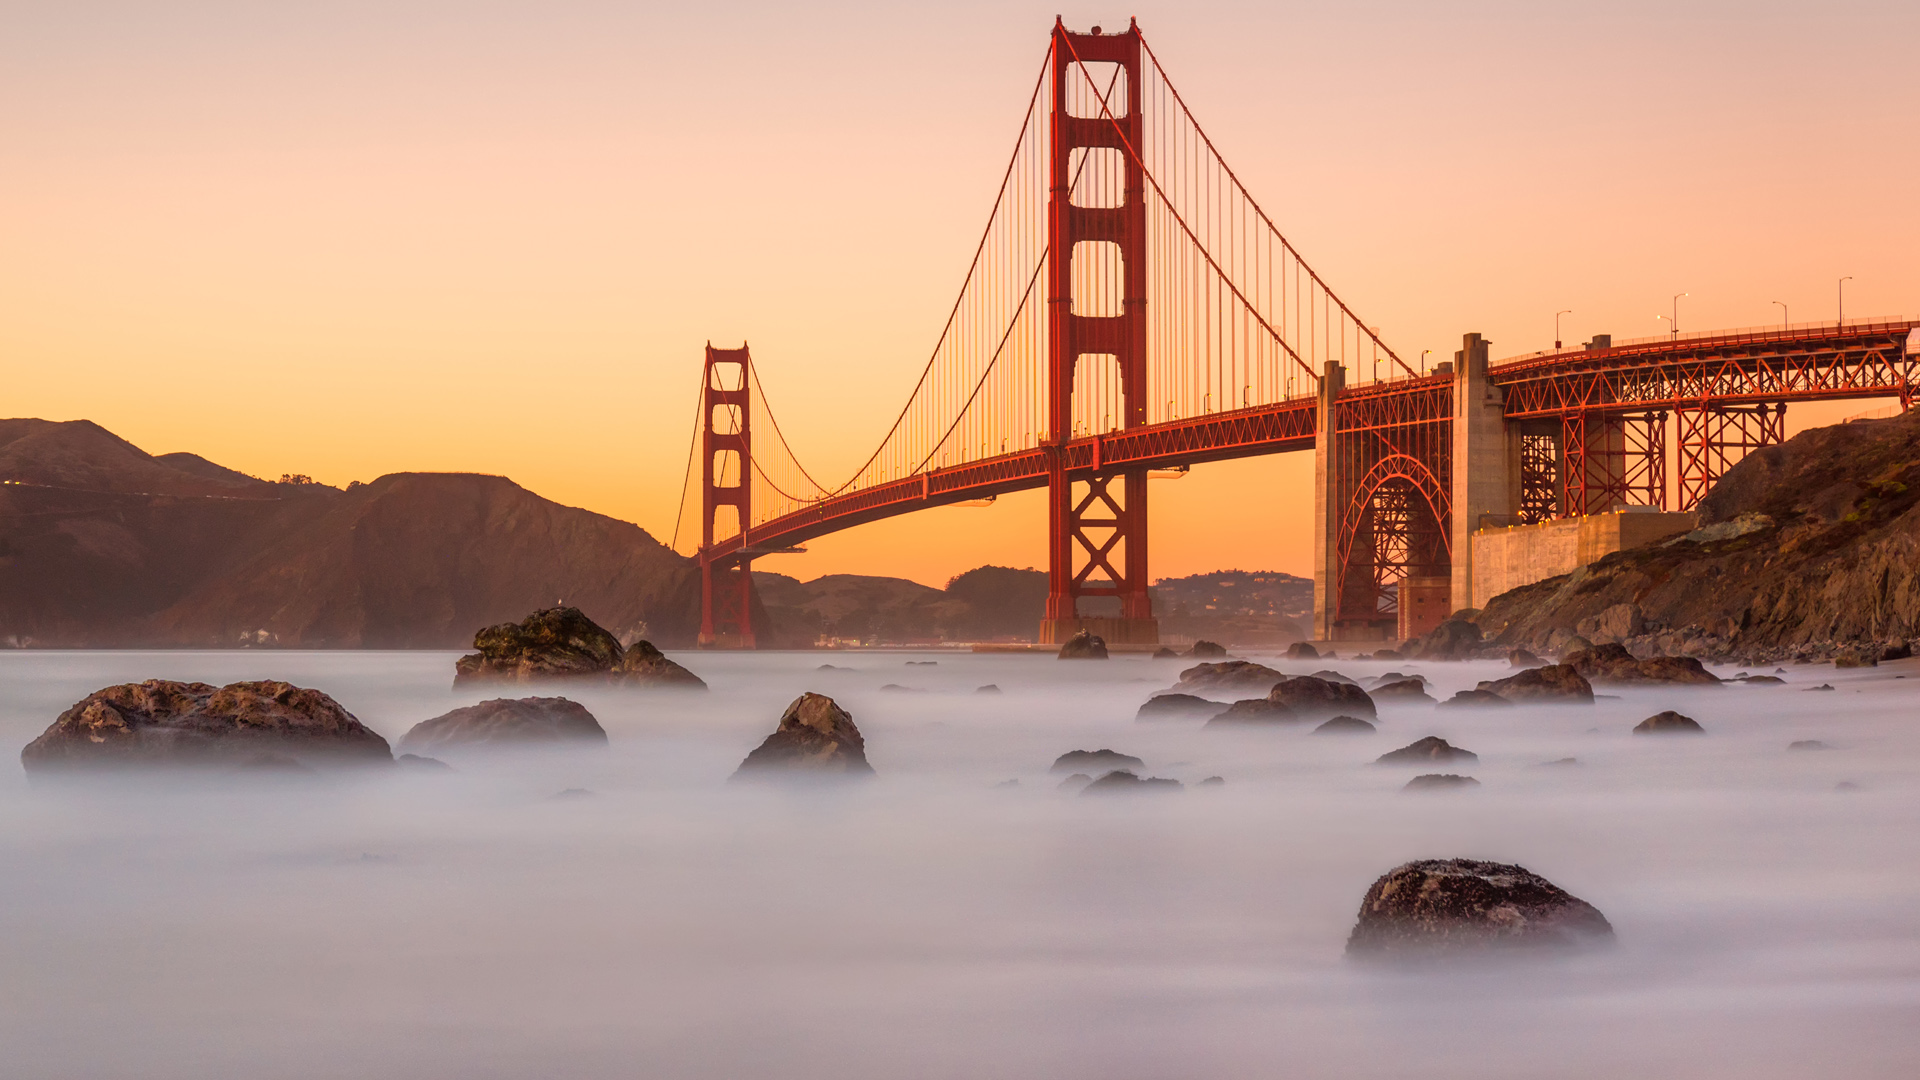
\includegraphics{./images/bridge_sunset.jpeg}

}

\caption{sunset on golden gate}

\end{figure}%

\section{Learning Objectives}\label{learning-objectives-8}

After this week's learning, student will be able to

\begin{enumerate}
\def\labelenumi{\arabic{enumi}.}
\tightlist
\item
  \emph{Describe} how sampling based uncertainty is reflected in OLS
  regression parameter estimates.
\item
  \emph{Report} standard errors, and \emph{conduct} tests for NHST of
  regression coefficients against zero.
\item
  \emph{Conduct} a regression based analysis, on real data, in ways that
  begin to explore regression as a modeling tool.
\end{enumerate}

\section{Class Announcements}\label{class-announcements-7}

\begin{enumerate}
\def\labelenumi{\arabic{enumi}.}
\tightlist
\item
  Congratulations on finishing your first lab!
\item
  The next (and the last) lab is coming up in two weeks.
\item
  Homework 09 has been assigned today, and it is due in a week.
\end{enumerate}

\section{Roadmap}\label{roadmap-5}

\textbf{Rear-View Mirror}

\begin{itemize}
\tightlist
\item
  Statisticians create a population model to represent the world.
\item
  Sometimes, the model includes an ``outcome'' random variable \(Y\) and
  ``input'' random variables \(X_1, X_2,...,X_k\).
\item
  The joint distribution of \(Y\) and \(X_1, X_2,...,X_k\) is
  complicated.
\item
  The best linear predictor (BLP) is the canonical way to summarize the
  relationship.
\item
  OLS provides a point estimate of the BLP
\end{itemize}

\textbf{Today}

\begin{itemize}
\tightlist
\item
  Robust Standard Error: quantify the uncertainty of OLS coefficients
\item
  Hypothesis testing with OLS coefficients
\item
  Bootstrapping
\end{itemize}

\textbf{Looking Ahead}

\begin{itemize}
\tightlist
\item
  Regression is a foundational tool that can be applied to different
  contexts
\item
  The process of building a regression model looks different, depending
  on whether the goal is prediction, description, or explanation.
\end{itemize}

\section{Uncertainty in OLS}\label{uncertainty-in-ols}

\subsection{Discussion Questions}\label{discussion-questions-1}

\begin{itemize}
\tightlist
\item
  List as many differences between the BLP and the OLS line as you can.
\item
  In the following regression table, explain in your own words what the
  standard error in parentheses means.
\end{itemize}

\begin{longtable}[]{@{}ll@{}}
\toprule\noalign{}
& outcome: sleep hours \\
\midrule\noalign{}
\endhead
\bottomrule\noalign{}
\endlastfoot
mg. melatonin & 0.52 \\
& (0.31) \\
\end{longtable}

\section{Understanding Uncertainty}\label{understanding-uncertainty}

Imagine three different regression models, each of the following form:

\[
  Y = 0 + \beta X + \epsilon
\]

The only difference is in the error term. The conditional distribution
is given by:

\begin{longtable}[]{@{}ll@{}}
\toprule\noalign{}
Model & Distribution of \(\epsilon\) cond. on \(X\) \\
\midrule\noalign{}
\endhead
\bottomrule\noalign{}
\endlastfoot
A & Uniform on \([-.5, +.5]\) \\
B & Uniform on \([ - |X|, |X| ]\) \\
C & Uniform on \([ -1 + |X|, 1- |X| ]\) \\
\end{longtable}

A is what we call a homoskedastic distribution. B and C are what we call
heteroskedastic. Below, we define R functions that simulate draws from
these three distributions.

\begin{Shaded}
\begin{Highlighting}[]
\NormalTok{rA }\OtherTok{\textless{}{-}} \ControlFlowTok{function}\NormalTok{(n, }\AttributeTok{slope=}\DecValTok{0}\NormalTok{)\{}
\NormalTok{  x       }\OtherTok{=} \FunctionTok{runif}\NormalTok{(n, }\AttributeTok{min =} \SpecialCharTok{{-}}\DecValTok{1}\NormalTok{,  }\AttributeTok{max =} \DecValTok{1}\NormalTok{)}
\NormalTok{  epsilon }\OtherTok{=} \FunctionTok{runif}\NormalTok{(n, }\AttributeTok{min =} \SpecialCharTok{{-}}\NormalTok{.}\DecValTok{5}\NormalTok{, }\AttributeTok{max =}\NormalTok{ .}\DecValTok{5}\NormalTok{)}
\NormalTok{  y       }\OtherTok{=} \DecValTok{0} \SpecialCharTok{+}\NormalTok{ slope}\SpecialCharTok{*}\NormalTok{x }\SpecialCharTok{+}\NormalTok{ epsilon}
  
  \FunctionTok{return}\NormalTok{(}
    \FunctionTok{data.frame}\NormalTok{(}\AttributeTok{x=}\NormalTok{x, }\AttributeTok{y=}\NormalTok{y)}
\NormalTok{    )}
\NormalTok{\}}

\NormalTok{rB }\OtherTok{\textless{}{-}} \ControlFlowTok{function}\NormalTok{(n, }\AttributeTok{slope=}\DecValTok{0}\NormalTok{)\{}
\NormalTok{  x       }\OtherTok{=} \FunctionTok{runif}\NormalTok{(n, }\AttributeTok{min =} \SpecialCharTok{{-}}\DecValTok{1}\NormalTok{, }\AttributeTok{max =} \DecValTok{1}\NormalTok{)}
\NormalTok{  epsilon }\OtherTok{=} \FunctionTok{runif}\NormalTok{(n, }\AttributeTok{min =} \SpecialCharTok{{-}} \FunctionTok{abs}\NormalTok{(x), }\AttributeTok{max =}\FunctionTok{abs}\NormalTok{(x))}
\NormalTok{  y       }\OtherTok{=} \DecValTok{0} \SpecialCharTok{+}\NormalTok{ slope}\SpecialCharTok{*}\NormalTok{x }\SpecialCharTok{+}\NormalTok{ epsilon}
  
  \FunctionTok{return}\NormalTok{(}
    \FunctionTok{data.frame}\NormalTok{(}\AttributeTok{x=}\NormalTok{x,}\AttributeTok{y=}\NormalTok{y)}
\NormalTok{    )}
\NormalTok{\}}

\NormalTok{rC }\OtherTok{\textless{}{-}} \ControlFlowTok{function}\NormalTok{(n, }\AttributeTok{slope=}\DecValTok{0}\NormalTok{)\{}
\NormalTok{  x       }\OtherTok{=} \FunctionTok{runif}\NormalTok{(n, }\AttributeTok{min =} \SpecialCharTok{{-}}\DecValTok{1}\NormalTok{, }\AttributeTok{max =} \DecValTok{1}\NormalTok{)}
\NormalTok{  epsilon }\OtherTok{=} \FunctionTok{runif}\NormalTok{(n, }\AttributeTok{min =} \SpecialCharTok{{-}}\DecValTok{1} \SpecialCharTok{+} \FunctionTok{abs}\NormalTok{(x), }\AttributeTok{max =} \DecValTok{1} \SpecialCharTok{{-}} \FunctionTok{abs}\NormalTok{(x))}
\NormalTok{  y       }\OtherTok{=} \DecValTok{0} \SpecialCharTok{+}\NormalTok{ slope}\SpecialCharTok{*}\NormalTok{x }\SpecialCharTok{+}\NormalTok{ epsilon}

  \FunctionTok{return}\NormalTok{(}
    \FunctionTok{data.frame}\NormalTok{(}\AttributeTok{x=}\NormalTok{x,}\AttributeTok{y=}\NormalTok{y)}
\NormalTok{    )}
\NormalTok{\}}
\end{Highlighting}
\end{Shaded}

\begin{Shaded}
\begin{Highlighting}[]
\NormalTok{data }\OtherTok{\textless{}{-}} \FunctionTok{rbind}\NormalTok{( }
  \FunctionTok{data.frame}\NormalTok{( }\FunctionTok{rA}\NormalTok{(}\DecValTok{200}\NormalTok{), }\AttributeTok{label =} \StringTok{\textquotesingle{}A\textquotesingle{}}\NormalTok{),}
  \FunctionTok{data.frame}\NormalTok{( }\FunctionTok{rB}\NormalTok{(}\DecValTok{200}\NormalTok{), }\AttributeTok{label =} \StringTok{\textquotesingle{}B\textquotesingle{}}\NormalTok{),}
  \FunctionTok{data.frame}\NormalTok{( }\FunctionTok{rC}\NormalTok{(}\DecValTok{200}\NormalTok{), }\AttributeTok{label =} \StringTok{\textquotesingle{}C\textquotesingle{}}\NormalTok{))}
\end{Highlighting}
\end{Shaded}

\begin{Shaded}
\begin{Highlighting}[]
\NormalTok{data }\SpecialCharTok{\%\textgreater{}\%} 
  \FunctionTok{ggplot}\NormalTok{(}\FunctionTok{aes}\NormalTok{(}\AttributeTok{x=}\NormalTok{x, }\AttributeTok{y=}\NormalTok{y)) }\SpecialCharTok{+} 
  \FunctionTok{geom\_point}\NormalTok{() }\SpecialCharTok{+} 
  \FunctionTok{lims}\NormalTok{(}
    \AttributeTok{x =} \FunctionTok{c}\NormalTok{(}\SpecialCharTok{{-}}\DecValTok{2}\NormalTok{,}\DecValTok{2}\NormalTok{), }
    \AttributeTok{y =} \FunctionTok{c}\NormalTok{(}\SpecialCharTok{{-}}\DecValTok{1}\NormalTok{,}\DecValTok{1}\NormalTok{)) }\SpecialCharTok{+} 
  \FunctionTok{labs}\NormalTok{(}\AttributeTok{title =} \StringTok{\textquotesingle{}Samples Drawn from Three Distributions\textquotesingle{}}\NormalTok{) }\SpecialCharTok{+} 
  \FunctionTok{facet\_grid}\NormalTok{(}\AttributeTok{rows=}\FunctionTok{vars}\NormalTok{(label))}
\end{Highlighting}
\end{Shaded}

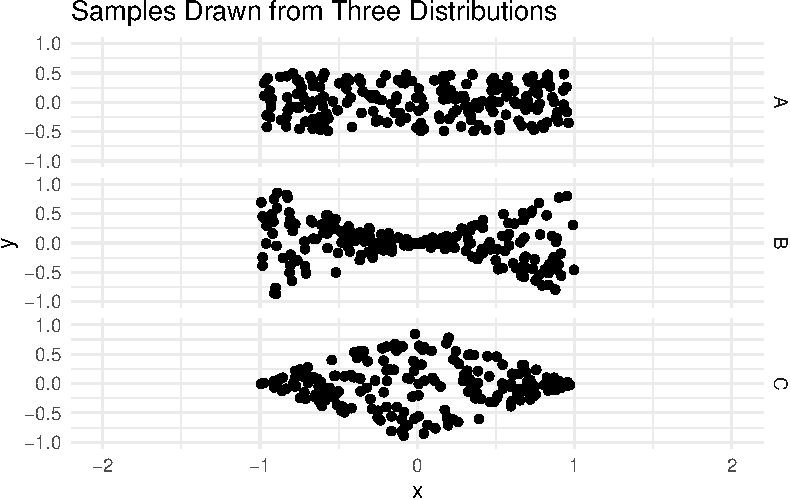
\includegraphics{09-regression-inference_files/figure-pdf/unnamed-chunk-3-1.pdf}

\subsection{Question 1}\label{question-1}

The following code draws a sample from distribution A, fits a regression
line, and plots it. Run it a few times to see what happens. Now explain
how you would visually estimate the standard error of the slope
coefficient. Why is this standard error important?

\begin{Shaded}
\begin{Highlighting}[]
\NormalTok{data }\OtherTok{\textless{}{-}}  \FunctionTok{rA}\NormalTok{(}\DecValTok{10}\NormalTok{, }\AttributeTok{slope=}\DecValTok{0}\NormalTok{)}

\NormalTok{data }\SpecialCharTok{\%\textgreater{}\%} 
  \FunctionTok{ggplot}\NormalTok{() }\SpecialCharTok{+} 
  \FunctionTok{aes}\NormalTok{(}\AttributeTok{x=}\NormalTok{x, }\AttributeTok{y=}\NormalTok{y) }\SpecialCharTok{+} 
  \FunctionTok{geom\_point}\NormalTok{() }\SpecialCharTok{+} 
  \FunctionTok{geom\_smooth}\NormalTok{(}\AttributeTok{method=}\StringTok{\textquotesingle{}lm\textquotesingle{}}\NormalTok{, }\AttributeTok{formula =} \StringTok{\textquotesingle{}y \textasciitilde{} x\textquotesingle{}}\NormalTok{, }\AttributeTok{se=}\ConstantTok{FALSE}\NormalTok{) }\SpecialCharTok{+} 
  \FunctionTok{lims}\NormalTok{(}
    \AttributeTok{x =} \FunctionTok{c}\NormalTok{(}\SpecialCharTok{{-}}\DecValTok{2}\NormalTok{,}\DecValTok{2}\NormalTok{), }
    \AttributeTok{y =} \FunctionTok{c}\NormalTok{(}\SpecialCharTok{{-}}\DecValTok{1}\NormalTok{,}\DecValTok{1}\NormalTok{)) }\SpecialCharTok{+} 
  \FunctionTok{labs}\NormalTok{(}\AttributeTok{title =} \StringTok{\textquotesingle{}Regression Fit to Distribution A\textquotesingle{}}\NormalTok{)}
\end{Highlighting}
\end{Shaded}

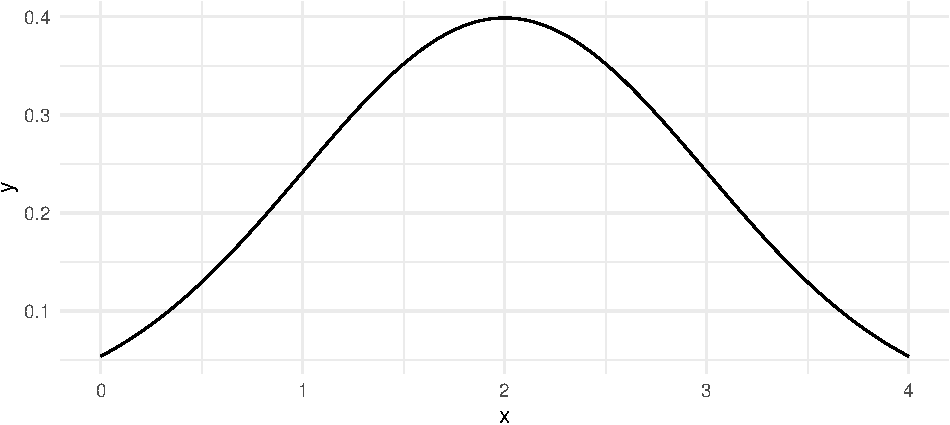
\includegraphics{09-regression-inference_files/figure-pdf/unnamed-chunk-4-1.pdf}

\begin{Shaded}
\begin{Highlighting}[]
\NormalTok{data\_points }\OtherTok{\textless{}{-}} \DecValTok{200}

\NormalTok{base\_plot\_a }\OtherTok{\textless{}{-}} \FunctionTok{rA}\NormalTok{(}\DecValTok{10}\NormalTok{) }\SpecialCharTok{\%\textgreater{}\%}  
  \FunctionTok{ggplot}\NormalTok{() }\SpecialCharTok{+} 
  \FunctionTok{aes}\NormalTok{(}\AttributeTok{x=}\NormalTok{x, }\AttributeTok{y=}\NormalTok{y) }\SpecialCharTok{+} 
  \FunctionTok{geom\_point}\NormalTok{() }\SpecialCharTok{+} 
  \FunctionTok{scale\_x\_continuous}\NormalTok{(}\AttributeTok{limits =} \FunctionTok{c}\NormalTok{(}\SpecialCharTok{{-}}\DecValTok{3}\NormalTok{, }\DecValTok{3}\NormalTok{))}

\ControlFlowTok{for}\NormalTok{(i }\ControlFlowTok{in} \DecValTok{1}\SpecialCharTok{:}\DecValTok{100}\NormalTok{) \{ }
\NormalTok{    base\_plot\_a }\OtherTok{\textless{}{-}}\NormalTok{ base\_plot\_a }\SpecialCharTok{+} \FunctionTok{rA}\NormalTok{(data\_points) }\SpecialCharTok{\%\textgreater{}\%} 
      \FunctionTok{stat\_smooth}\NormalTok{(}
        \AttributeTok{mapping =} \FunctionTok{aes}\NormalTok{(}\AttributeTok{x=}\NormalTok{x, }\AttributeTok{y=}\NormalTok{y), }
        \AttributeTok{method  =} \StringTok{\textquotesingle{}lm\textquotesingle{}}\NormalTok{,         }\AttributeTok{se =} \ConstantTok{FALSE}\NormalTok{, }
        \AttributeTok{formula =} \StringTok{\textquotesingle{}y\textasciitilde{}x\textquotesingle{}}\NormalTok{, }\AttributeTok{fullrange =} \ConstantTok{TRUE}\NormalTok{,}
        \AttributeTok{color   =} \StringTok{\textquotesingle{}grey\textquotesingle{}}\NormalTok{,    }\AttributeTok{alpha =} \FloatTok{0.5}\NormalTok{,}
        \AttributeTok{size    =} \FloatTok{0.5}
\NormalTok{      )}
\NormalTok{\}}
\end{Highlighting}
\end{Shaded}

\begin{verbatim}
Warning: Using `size` aesthetic for lines was deprecated in ggplot2 3.4.0.
i Please use `linewidth` instead.
\end{verbatim}

\begin{Shaded}
\begin{Highlighting}[]
\NormalTok{base\_plot\_b }\OtherTok{\textless{}{-}} \FunctionTok{rB}\NormalTok{(}\DecValTok{10}\NormalTok{) }\SpecialCharTok{\%\textgreater{}\%}  
  \FunctionTok{ggplot}\NormalTok{() }\SpecialCharTok{+} 
  \FunctionTok{aes}\NormalTok{(}\AttributeTok{x=}\NormalTok{x, }\AttributeTok{y=}\NormalTok{y) }\SpecialCharTok{+} 
  \FunctionTok{geom\_point}\NormalTok{() }\SpecialCharTok{+} 
  \FunctionTok{scale\_x\_continuous}\NormalTok{(}\AttributeTok{limits =} \FunctionTok{c}\NormalTok{(}\SpecialCharTok{{-}}\DecValTok{3}\NormalTok{, }\DecValTok{3}\NormalTok{))}

\ControlFlowTok{for}\NormalTok{(i }\ControlFlowTok{in} \DecValTok{1}\SpecialCharTok{:}\DecValTok{100}\NormalTok{) \{ }
\NormalTok{    base\_plot\_b }\OtherTok{\textless{}{-}}\NormalTok{ base\_plot\_b }\SpecialCharTok{+} \FunctionTok{rB}\NormalTok{(data\_points) }\SpecialCharTok{\%\textgreater{}\%} 
      \FunctionTok{stat\_smooth}\NormalTok{(}
        \AttributeTok{mapping =} \FunctionTok{aes}\NormalTok{(}\AttributeTok{x=}\NormalTok{x, }\AttributeTok{y=}\NormalTok{y), }
        \AttributeTok{method  =} \StringTok{\textquotesingle{}lm\textquotesingle{}}\NormalTok{,         }\AttributeTok{se =} \ConstantTok{FALSE}\NormalTok{, }
        \AttributeTok{formula =} \StringTok{\textquotesingle{}y\textasciitilde{}x\textquotesingle{}}\NormalTok{, }\AttributeTok{fullrange =} \ConstantTok{TRUE}\NormalTok{,}
        \AttributeTok{color   =} \StringTok{\textquotesingle{}grey\textquotesingle{}}\NormalTok{,    }\AttributeTok{alpha =} \FloatTok{0.5}\NormalTok{,}
        \AttributeTok{size    =} \FloatTok{0.5}
\NormalTok{      )}
\NormalTok{  \}}

\NormalTok{base\_plot\_c }\OtherTok{\textless{}{-}} \FunctionTok{rC}\NormalTok{(}\DecValTok{10}\NormalTok{) }\SpecialCharTok{\%\textgreater{}\%}  
  \FunctionTok{ggplot}\NormalTok{() }\SpecialCharTok{+} 
  \FunctionTok{aes}\NormalTok{(}\AttributeTok{x=}\NormalTok{x, }\AttributeTok{y=}\NormalTok{y) }\SpecialCharTok{+} 
  \FunctionTok{geom\_point}\NormalTok{() }\SpecialCharTok{+} 
  \FunctionTok{scale\_x\_continuous}\NormalTok{(}\AttributeTok{limits =} \FunctionTok{c}\NormalTok{(}\SpecialCharTok{{-}}\DecValTok{3}\NormalTok{, }\DecValTok{3}\NormalTok{))}

\ControlFlowTok{for}\NormalTok{(i }\ControlFlowTok{in} \DecValTok{1}\SpecialCharTok{:}\DecValTok{100}\NormalTok{) \{ }
\NormalTok{    base\_plot\_c }\OtherTok{\textless{}{-}}\NormalTok{ base\_plot\_c }\SpecialCharTok{+} \FunctionTok{rC}\NormalTok{(data\_points) }\SpecialCharTok{\%\textgreater{}\%} 
      \FunctionTok{stat\_smooth}\NormalTok{(}
        \AttributeTok{mapping =} \FunctionTok{aes}\NormalTok{(}\AttributeTok{x=}\NormalTok{x, }\AttributeTok{y=}\NormalTok{y), }
        \AttributeTok{method  =} \StringTok{\textquotesingle{}lm\textquotesingle{}}\NormalTok{,         }\AttributeTok{se =} \ConstantTok{FALSE}\NormalTok{, }
        \AttributeTok{formula =} \StringTok{\textquotesingle{}y\textasciitilde{}x\textquotesingle{}}\NormalTok{, }\AttributeTok{fullrange =} \ConstantTok{TRUE}\NormalTok{,}
        \AttributeTok{color   =} \StringTok{\textquotesingle{}grey\textquotesingle{}}\NormalTok{,    }\AttributeTok{alpha =} \FloatTok{0.5}\NormalTok{,}
        \AttributeTok{size    =} \FloatTok{0.5}
\NormalTok{      )}
\NormalTok{\}}

\NormalTok{base\_plot\_a }\SpecialCharTok{+}\NormalTok{ base\_plot\_b }\SpecialCharTok{+}\NormalTok{ base\_plot\_c }\SpecialCharTok{+}\NormalTok{ patchwork}\SpecialCharTok{::}\FunctionTok{plot\_layout}\NormalTok{(}\AttributeTok{axes =} \StringTok{"collect"}\NormalTok{)}
\end{Highlighting}
\end{Shaded}

\includegraphics{09-regression-inference_files/figure-pdf/unnamed-chunk-5-1.pdf}

\begin{Shaded}
\begin{Highlighting}[]
\NormalTok{?}\FunctionTok{plot\_layout}\NormalTok{()}
\end{Highlighting}
\end{Shaded}

\subsection{Question 2}\label{question-2}

You have a sample from each distribution, A, B, and C and you fit a
regression of Y on X. Which will have the highest standard error for the
slope coefficient? Which will have the lowest standard error? Why? (You
may want to try experimenting with the function defined above)

\subsection{Question 3}\label{question-3}

For distribution A, perform a simulated experiment. Draw a large number
of samples, and for each sample fit a linear regression. Store the slope
coefficient from each regression in a vector. Finally, compute the
standard deviation for the slope coefficients.

Repeat this process for distributions B and C. Do the results match your
intuition?

\section{Understanding Uncertainty}\label{understanding-uncertainty-1}

Under the relatively stricter assumptions of constant error variance,
the variance of a slope coefficient is given by

\[
  V(\hat{\beta_j}) = \frac{\sigma^2}{SST_j (1-R_j^2)}
\]

A similar formulation is given in \emph{FOAS} as definition 4.2.3,

\[
  \hat{V}_{C}[\hat{\beta}] = \hat{\sigma}^2 \left( X^{T} X \right)^{-1} \rightsquigarrow \hat{\sigma}^{2}{\left(\mathbb{X}^{T}\mathbb{X}\right)}, 
\] where \(\hat{\sigma}^{2} = V[\hat{\epsilon}]\)

Explain why each term makes the variance higher or lower:

\begin{itemize}
\tightlist
\item
  \(\hat{\sigma}^2\) is the variance of the error \(\hat{\epsilon}\)
\item
  \(SST_j\) is (unscaled) variance of \(X_j\)
\item
  \(R_j^2\) is \(R^2\) for a regression of \(X_j\) on the other \(X\)'s
\end{itemize}

\section{R Exercise}\label{r-exercise-1}

\textbf{Real Estate in Boston}

The file \texttt{hprice1.RData} contains 88 observations of homes in the
Boston area, taken from the real estate pages of the Boston Globe during
1990. This data was provided by Wooldridge.

\begin{Shaded}
\begin{Highlighting}[]
\FunctionTok{load}\NormalTok{(}\StringTok{\textquotesingle{}data/hprice1.RData\textquotesingle{}}\NormalTok{) }\CommentTok{\# provides 3 objects }
\end{Highlighting}
\end{Shaded}

Last week, we fit a regression of price on square feet.

\begin{Shaded}
\begin{Highlighting}[]
\NormalTok{model\_one }\OtherTok{\textless{}{-}} \FunctionTok{lm}\NormalTok{(price }\SpecialCharTok{\textasciitilde{}}\NormalTok{ sqrft, }\AttributeTok{data =}\NormalTok{ data)}
\NormalTok{model\_one}\SpecialCharTok{$}\NormalTok{df.residual}
\end{Highlighting}
\end{Shaded}

\begin{verbatim}
[1] 86
\end{verbatim}

Can you use the pieces that you're familiar with to produce a p-value
using robust standard errors?

\begin{Shaded}
\begin{Highlighting}[]
\NormalTok{regression\_p\_value }\OtherTok{\textless{}{-}} \ControlFlowTok{function}\NormalTok{(model, variable) \{ }
  \DocumentationTok{\#\# this function takes a model }
  \DocumentationTok{\#\# and computes a test{-}statistic, }
  \DocumentationTok{\#\# then compares that test{-}statistic against the }
  \DocumentationTok{\#\# appropriate t{-}distribution}
  
  \DocumentationTok{\#\# you can use the following helper functions: }
  \DocumentationTok{\#\#  {-} coef()}
  \DocumentationTok{\#\#  {-} vcovHC()}
\NormalTok{  df }\OtherTok{\textless{}{-}}\NormalTok{ model}\SpecialCharTok{$}\NormalTok{df.residual}
  
  \CommentTok{\# numerator   \textless{}{-} \textquotesingle{}fill this in\textquotesingle{}}
  \CommentTok{\# denominator \textless{}{-} \textquotesingle{}fill this in\textquotesingle{}}
  
\NormalTok{  numerator   }\OtherTok{\textless{}{-}} \FunctionTok{coef}\NormalTok{(model)[variable]}
\NormalTok{  denominator }\OtherTok{\textless{}{-}} \FunctionTok{sqrt}\NormalTok{(}\FunctionTok{diag}\NormalTok{(}\FunctionTok{vcovHC}\NormalTok{(model)))[variable]}
  
\NormalTok{  test\_stat\_  }\OtherTok{\textless{}{-}}\NormalTok{ numerator }\SpecialCharTok{/}\NormalTok{ denominator}
\NormalTok{  p\_val\_      }\OtherTok{\textless{}{-}} \StringTok{\textquotesingle{}fill this in\textquotesingle{}}
\NormalTok{  p\_val\_      }\OtherTok{\textless{}{-}} \FunctionTok{pt}\NormalTok{(test\_stat\_, }\AttributeTok{df =}\NormalTok{ df, }\AttributeTok{lower.tail =} \ConstantTok{FALSE}\NormalTok{) }\SpecialCharTok{*} \DecValTok{2}
  
  \FunctionTok{return}\NormalTok{(p\_val\_)}
\NormalTok{  \}}
\end{Highlighting}
\end{Shaded}

If you want to confirm that what you have written is correct, you can
compare against the value that you receive from the line below.

\begin{Shaded}
\begin{Highlighting}[]
\FunctionTok{coeftest}\NormalTok{(model\_one, }\AttributeTok{vcov. =} \FunctionTok{vcovHC}\NormalTok{(model\_one))}
\end{Highlighting}
\end{Shaded}

\begin{verbatim}

t test of coefficients:

             Estimate Std. Error t value  Pr(>|t|)    
(Intercept) 11.204145  39.450563  0.2840    0.7771    
sqrft        0.140211   0.021111  6.6417 2.673e-09 ***
---
Signif. codes:  0 '***' 0.001 '**' 0.01 '*' 0.05 '.' 0.1 ' ' 1
\end{verbatim}

\begin{Shaded}
\begin{Highlighting}[]
\NormalTok{p\_value\_ }\OtherTok{\textless{}{-}}\NormalTok{ broom}\SpecialCharTok{::}\FunctionTok{tidy}\NormalTok{(}\FunctionTok{coeftest}\NormalTok{(model\_one, }\AttributeTok{vcov. =} \FunctionTok{vcovHC}\NormalTok{(model\_one))) }\SpecialCharTok{\%\textgreater{}\%} 
  \FunctionTok{filter}\NormalTok{(term }\SpecialCharTok{==} \StringTok{\textquotesingle{}sqrft\textquotesingle{}}\NormalTok{) }\SpecialCharTok{\%\textgreater{}\%} 
  \FunctionTok{select}\NormalTok{(}\StringTok{\textquotesingle{}p.value\textquotesingle{}}\NormalTok{) }\SpecialCharTok{\%\textgreater{}\%} 
  \FunctionTok{as.numeric}\NormalTok{()}

\FunctionTok{test\_that}\NormalTok{(}
  \StringTok{\textquotesingle{}test that hand coded p{-}value is the same as the pre{-}rolled\textquotesingle{}}\NormalTok{, }
  \FunctionTok{expect\_equal}\NormalTok{(}
    \AttributeTok{object   =} \FunctionTok{as.numeric}\NormalTok{(}\FunctionTok{regression\_p\_value}\NormalTok{(model\_one, }\StringTok{\textquotesingle{}sqrft\textquotesingle{}}\NormalTok{)), }
    \AttributeTok{expected =}\NormalTok{ p\_value\_}
\NormalTok{  )}
\NormalTok{)}
\end{Highlighting}
\end{Shaded}

\begin{verbatim}
Test passed 
\end{verbatim}

\textbf{Questions}

\begin{enumerate}
\def\labelenumi{\arabic{enumi}.}
\tightlist
\item
  Estimate a new model (and save it into another object) that includes
  the size of the lot and whether the house is a colonial. This will
  estimate the model:
\end{enumerate}

\[
  price = \beta_{0} + \beta_{1} sqrft + \beta_{2} lotsize + \beta_{3} colonial? + e
\]

\begin{itemize}
\tightlist
\item
  \emph{BUT BEFORE YOU DO}, make a prediction: What do you think is
  going to happen to the coefficient that relates square footage and
  price?

  \begin{itemize}
  \tightlist
  \item
    Will the coefficient increase, decrease, or stay the same?
  \item
    Will the \emph{uncertainty} about the coefficient increase,
    decrease, or stay the same?
  \item
    Conduct an F-test that evaluates whether the model \emph{as a whole}
    does better when the coefficients on \texttt{colonial} and
    \texttt{lotsize} are allowed to estimate freely, or instead are
    restricted to be zero (i.e.~\(\beta_{2} = \beta_{3} = 0\).
  \end{itemize}
\end{itemize}

\begin{enumerate}
\def\labelenumi{\arabic{enumi}.}
\setcounter{enumi}{1}
\tightlist
\item
  Use the function \texttt{vcovHC} from the \texttt{sandwich} package to
  estimate (a) the the heteroskedastic consistent (i.e.~``robust'')
  variance covariance matrix; and (b) the robust standard errors for the
  intercept and slope of this regression. Recall, what is the
  relationship between the VCOV and SE in a regression?
\end{enumerate}

\begin{enumerate}
\def\labelenumi{\arabic{enumi}.}
\setcounter{enumi}{2}
\tightlist
\item
  Perform a hypothesis test to check whether the population relationship
  between \texttt{sqrft} and \texttt{price} is zero. Use
  \texttt{coeftest()} with the robust standard errors computed above.
\end{enumerate}

\begin{enumerate}
\def\labelenumi{\arabic{enumi}.}
\setcounter{enumi}{3}
\item
  Use the robust standard error and \texttt{qt} to compute a 95\%
  confidence interval for the coefficient \texttt{sqrft} in the second
  model that you estimated.
  \(price = \beta_{0} + \beta_{1} sqrft + \beta_{2} lotsize + \beta_{3} colonial\).
\item
  \textbf{Bootstrap.} The book \emph{very} quickly talks about
  bootstrapping which is the process of sampling \emph{with replacement}
  and fitting a model. The idea behind the bootstrap is that since the
  data is generated via an iid sample from the population, that you can
  simulate re-running your analysis by drawing repeated samples from the
  data that you have.
\end{enumerate}

Below is code that will conduct a boostrapping estimator of the
uncertainty of the \texttt{sqrft} variable when \texttt{lotsize} and
\texttt{colonial} are included in the model.

\begin{Shaded}
\begin{Highlighting}[]
\NormalTok{bootstrap\_sqft }\OtherTok{\textless{}{-}} \ControlFlowTok{function}\NormalTok{(}\AttributeTok{d =}\NormalTok{ data, }\AttributeTok{number\_of\_bootstraps =} \DecValTok{1000}\NormalTok{) \{ }
\NormalTok{  number\_of\_rows }\OtherTok{\textless{}{-}} \FunctionTok{nrow}\NormalTok{(d)}

\NormalTok{    coef\_sqft }\OtherTok{\textless{}{-}} \FunctionTok{rep}\NormalTok{(}\ConstantTok{NA}\NormalTok{, number\_of\_bootstraps)}

    \ControlFlowTok{for}\NormalTok{(i }\ControlFlowTok{in} \DecValTok{1}\SpecialCharTok{:}\NormalTok{number\_of\_bootstraps) \{ }
\NormalTok{      bootstrap\_data }\OtherTok{\textless{}{-}}\NormalTok{ d[}\FunctionTok{sample}\NormalTok{(}\AttributeTok{x=}\DecValTok{1}\SpecialCharTok{:}\NormalTok{number\_of\_rows, }\AttributeTok{size=}\NormalTok{number\_of\_rows, }\AttributeTok{replace=}\ConstantTok{TRUE}\NormalTok{), ]  }
\NormalTok{      estimated\_model }\OtherTok{\textless{}{-}} \FunctionTok{lm}\NormalTok{(price }\SpecialCharTok{\textasciitilde{}}\NormalTok{ sqrft, }\AttributeTok{data =}\NormalTok{ bootstrap\_data)}
\NormalTok{      coef\_sqft[i]    }\OtherTok{\textless{}{-}} \FunctionTok{coef}\NormalTok{(estimated\_model)[}\StringTok{\textquotesingle{}sqrft\textquotesingle{}}\NormalTok{]}
\NormalTok{    \}}
  \FunctionTok{return}\NormalTok{(coef\_sqft)}
\NormalTok{\}}
\end{Highlighting}
\end{Shaded}

\begin{Shaded}
\begin{Highlighting}[]
\NormalTok{bootstrap\_result }\OtherTok{\textless{}{-}} \FunctionTok{bootstrap\_sqft}\NormalTok{(}\AttributeTok{d =}\NormalTok{ data, }\AttributeTok{number\_of\_bootstraps =} \DecValTok{10000}\NormalTok{)}
\end{Highlighting}
\end{Shaded}

With this, it is possible to plot the distribution of these regression
coefficients:

\begin{Shaded}
\begin{Highlighting}[]
\FunctionTok{ggplot}\NormalTok{() }\SpecialCharTok{+} 
  \FunctionTok{aes}\NormalTok{(}\AttributeTok{x =}\NormalTok{ bootstrap\_result) }\SpecialCharTok{+} 
  \FunctionTok{geom\_histogram}\NormalTok{() }\SpecialCharTok{+} 
  \FunctionTok{labs}\NormalTok{(}
    \AttributeTok{x =} \StringTok{\textquotesingle{}Estimated Coefficient\textquotesingle{}}\NormalTok{, }
    \AttributeTok{y =} \StringTok{\textquotesingle{}Count\textquotesingle{}}\NormalTok{, }
    \AttributeTok{title =} \StringTok{\textquotesingle{}Bootstrap coefficients for square footage\textquotesingle{}}
\NormalTok{  )}
\end{Highlighting}
\end{Shaded}

\begin{verbatim}
`stat_bin()` using `bins = 30`. Pick better value with `binwidth`.
\end{verbatim}

\includegraphics{09-regression-inference_files/figure-pdf/unnamed-chunk-14-1.pdf}

Compute the standard deviation of the bootstrapped regression
coefficients. How does this compare to the robust standard errors you
computed above?

\begin{Shaded}
\begin{Highlighting}[]
\FunctionTok{coeftest}\NormalTok{(model\_one, }\AttributeTok{vcov. =} \FunctionTok{vcovHC}\NormalTok{(model\_one))}
\end{Highlighting}
\end{Shaded}

\begin{verbatim}

t test of coefficients:

             Estimate Std. Error t value  Pr(>|t|)    
(Intercept) 11.204145  39.450563  0.2840    0.7771    
sqrft        0.140211   0.021111  6.6417 2.673e-09 ***
---
Signif. codes:  0 '***' 0.001 '**' 0.01 '*' 0.05 '.' 0.1 ' ' 1
\end{verbatim}

\begin{Shaded}
\begin{Highlighting}[]
\FunctionTok{sd}\NormalTok{(bootstrap\_result)}
\end{Highlighting}
\end{Shaded}

\begin{verbatim}
[1] 0.01993763
\end{verbatim}

\chapter{Descriptive Model Building}\label{descriptive-model-building}

\begin{Shaded}
\begin{Highlighting}[]
\FunctionTok{library}\NormalTok{(tidyverse)}
\end{Highlighting}
\end{Shaded}

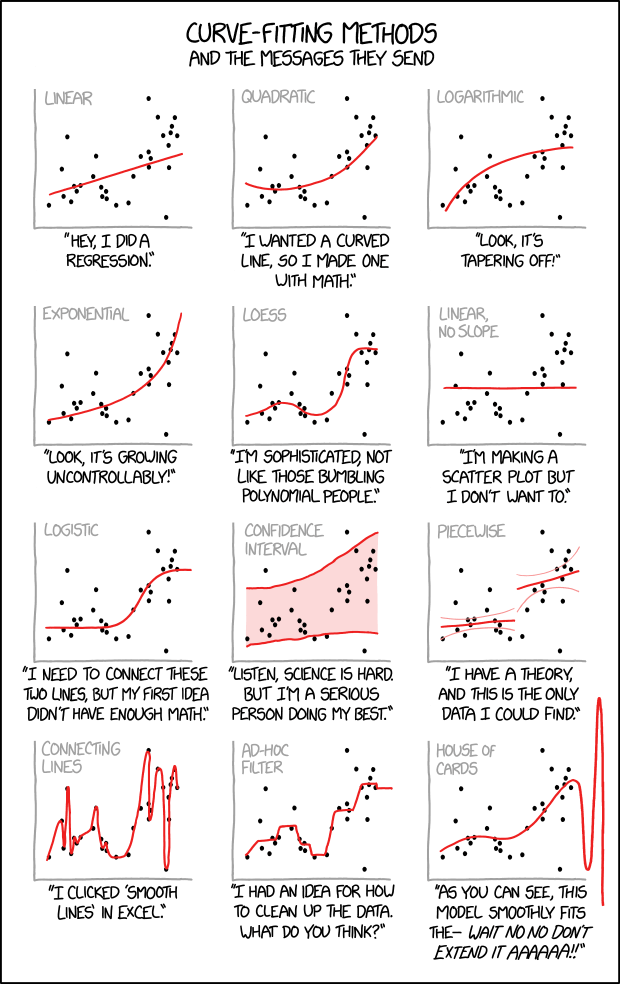
\includegraphics[width=0.8\textwidth,height=\textheight]{./images/curve_fitting.png}

\section{Learning Objectives}\label{learning-objectives-9}

\begin{enumerate}
\def\labelenumi{\arabic{enumi}.}
\tightlist
\item
  \textbf{Understand} that models don't know what they're doing, and it
  is the role of the data scientist to control and deploy them.
\item
  \textbf{Practice} transforming variables, on the fly, at the time of
  regression modeling in order to produce an effective,
  \emph{descriptive} regression model.
\item
  \textbf{Appreciate} that the random variable understanding of the
  world that we have constructed is useful for thinking of reshaping, or
  transforming spaces.
\end{enumerate}

\section{Class Announcements}\label{class-announcements-8}

\begin{enumerate}
\def\labelenumi{\arabic{enumi}.}
\tightlist
\item
  The Regression Lab begins next week.

  \begin{itemize}
  \tightlist
  \item
    Your instructor will divide you into teams.
  \item
    As part of the lab, you will perform a statistical analysis using
    linear regression models.
  \end{itemize}
\end{enumerate}

\section{Roadmap}\label{roadmap-6}

\textbf{Rearview Mirror}

\begin{itemize}
\item
  Statisticians create a population model to represent the world.
\item
  The BLP is a useful way to summarize the relationship between one
  outcome random variable \(Y\) and input random varibles
  \(X_1,...,X_k\)
\item
  OLS regression is an estimator for the Best Linear Predictor (BLP)
\item
  We can capture the sampling uncertainty in an OLS regression with
  standard errors, and tests for model parameters.
\end{itemize}

\textbf{Today}

\begin{itemize}
\item
  The research goal determines the strategy for building a linear model.
\item
  Description means summarizing or representing data in a compact,
  human-understandable way.
\item
  We will capture complex relationships by transforming data, including
  using indicator variables and interaction terms.
\end{itemize}

\textbf{Looking Ahead}

\begin{itemize}
\item
  We will see how model building for explanation is different from
  building for description.
\item
  The famous Classical Linear Model (CLM) allows us to apply regression
  to smaller samples.
\end{itemize}

\section{Discussion}\label{discussion}

\subsection{Three modes of model
building}\label{three-modes-of-model-building}

\begin{itemize}
\tightlist
\item
  Recall the three major modes of model building: Prediction,
  Description, Explanation.
\item
  What is the appropriate mode for each of the following questions?
\end{itemize}

\begin{enumerate}
\def\labelenumi{\arabic{enumi}.}
\tightlist
\item
  What is going on?
\item
  Why is something going on?
\item
  What is going to happen?
\end{enumerate}

\begin{itemize}
\tightlist
\item
  Think of a research question you are interested in. Which mode is it
  aligned with?
\end{itemize}

\subsection{The statistical modeling process in different
modes}\label{the-statistical-modeling-process-in-different-modes}

\begin{itemize}
\item
  How does the modeling goal influence each of the following steps in
  the statistical modeling process?

  \begin{itemize}
  \item
    Choice of variables and transformation
  \item
    Choice of model (ols regression, neural nets, random forest, etc.)
  \item
    Model evaluation
  \end{itemize}
\end{itemize}

\section{R Activity: Measuring the return to
education}\label{r-activity-measuring-the-return-to-education}

\begin{itemize}
\tightlist
\item
  In labor economics, a key concept is \emph{returns to education}.\\
\item
  Our goal is description: what is the relationship between education
  and wages? We will proceed in two steps:

  \begin{itemize}
  \tightlist
  \item
    First, we will discuss what the appropriate specifications are.
  \item
    Then we will estimate the different models to answer this question.
  \end{itemize}
\item
  We will use wage1 dataset in the wooldridge package in the following
  sections.
\end{itemize}

\begin{Shaded}
\begin{Highlighting}[]
\NormalTok{wage1 }\OtherTok{\textless{}{-}}\NormalTok{ wooldridge}\SpecialCharTok{::}\NormalTok{wage1}
\CommentTok{\#names(wage1)}

\NormalTok{wage1 }\SpecialCharTok{|\textgreater{}} 
  \FunctionTok{ggplot}\NormalTok{() }\SpecialCharTok{+} 
  \FunctionTok{aes}\NormalTok{(}\AttributeTok{x=}\NormalTok{wage) }\SpecialCharTok{+} 
  \FunctionTok{geom\_histogram}\NormalTok{()}
\end{Highlighting}
\end{Shaded}

\begin{verbatim}
`stat_bin()` using `bins = 30`. Pick better value with `binwidth`.
\end{verbatim}

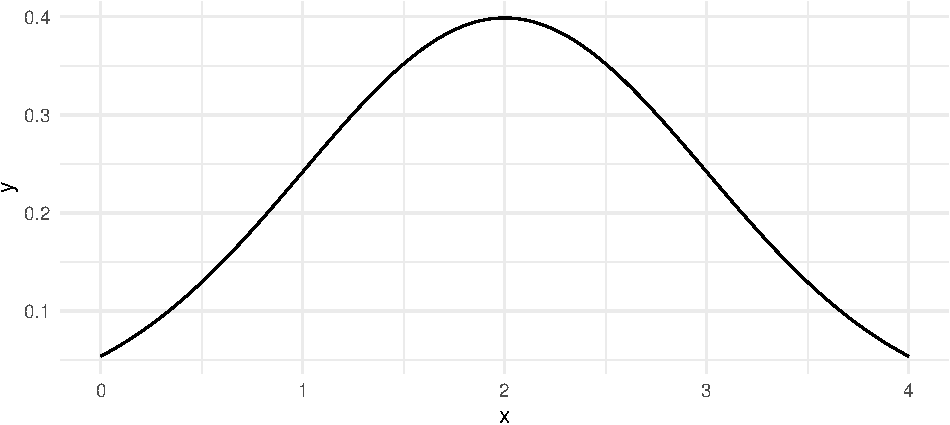
\includegraphics{10-descriptive-models_files/figure-pdf/unnamed-chunk-2-1.pdf}

\subsection{Transformations}\label{transformations}

\subsubsection{Applying and Interpreting
Logarithms}\label{applying-and-interpreting-logarithms}

\begin{itemize}
\item
  Which of the following specifications best capture the relationship
  between education and hourly wage? (Hint: Do a quick a EDA)

  \begin{itemize}
  \tightlist
  \item
    level-level: \(wage = \beta_0 + \beta_1 educ + u\)
  \item
    Level-log: \(wage = \beta_0 + \beta_1 \ln(educ)  + u\)
  \item
    log-level: \(\ln(wage) = \beta_0 + \beta_1 educ + u\)
  \item
    log-log: \(\ln(wage) = \beta_0 + \beta_1 \ln(educ) + u\)
  \end{itemize}
\item
  What is the interpretation of \(\beta_0\) and \(\beta_1\) in your
  selected specification?
\item
  Can we use \(R^2\) or Adjusted \(R^2\) to choose between level-level
  or log-level specifications?
\end{itemize}

\textbf{Remember}

\begin{itemize}
\tightlist
\item
  \textbf{Doing a log transformation for any reason essentially implies
  a fundamentally different relationship between outcome (Y) and
  predictor (X) that we need to capture}
\end{itemize}

\subsubsection{Applying and Interpreting
Polynomials}\label{applying-and-interpreting-polynomials}

\begin{itemize}
\item
  The following specifications include two control variables: years of
  experience (exper) and years at current company (tenure).
\item
  Do a quick EDA and select the specification that better suits our
  description goal.

  \begin{itemize}
  \item
    \(wage = \beta_0 + \beta_1 educ + \beta_2 exper + \beta_3 tenure + u\)
  \item
    \(\begin{aligned}
    wage &= \beta_0 + \beta_1 educ + \beta_2 exper + \beta_3 exper^2 + \\
    & \beta_4 tenure + \beta_5 tenure^2 + u
    \end{aligned}\)
  \end{itemize}
\item
  How do you interpret the \(\beta\) coefficients?
\end{itemize}

\subsubsection{Applying and Interpreting Indicator variables and
interaction
terms}\label{applying-and-interpreting-indicator-variables-and-interaction-terms}

\begin{itemize}
\item
  In the following models, first, explain why the indicator variables or
  interaction terms have been included. Then identify the reference
  group (if any) and interpret all coefficients.

  \begin{itemize}
  \item
    \(wage = \beta_0 + \beta_1 educ + \beta_2 I(educ \geq 12) + u\)
  \item
    \(wage = \beta_0 + \beta_1 educ + \beta_2 female + u\)
  \item
    \(wage = \beta_0 + \beta_1 educ + \beta_2 female + \beta_3 educ*female + u\)
  \item
    \(\begin{aligned}
    wage &= \beta_0 + \beta_1 female + \beta_2 I(educ = 2) + \beta_3 I(educ = 3)\\
    &...+ \beta_{20} I(educ = 20) + u\\
    \end{aligned}\)
  \end{itemize}
\end{itemize}

\subsection{Estimation}\label{estimation}

\textbf{Estimating Returns to Education}

\begin{itemize}
\tightlist
\item
  Answer the following questions using an appropriate hypothesis test.

  \begin{enumerate}
  \def\labelenumi{\arabic{enumi}.}
  \tightlist
  \item
    Is a year of education associated with changes to hourly wage?
    (Include experience and tenure without polynomial terms).
  \item
    Is the association between wage and experience / wage and tenure
    non-linear?
  \item
    Is there evidence for gender wage discrimination in the U.S.?
  \item
    Is there any evidence for a graduation effect on wage?
  \end{enumerate}
\item
  Display all estimated models in a regression table, and discuss the
  robustness of your results.
\end{itemize}

\chapter{Explanatory Model Building}\label{explanatory-model-building}

\begin{Shaded}
\begin{Highlighting}[]
\FunctionTok{library}\NormalTok{(tidyverse)}
\FunctionTok{library}\NormalTok{(patchwork)}

\FunctionTok{theme\_set}\NormalTok{(}\FunctionTok{theme\_minimal}\NormalTok{())}
\end{Highlighting}
\end{Shaded}

\begin{figure}[H]

{\centering 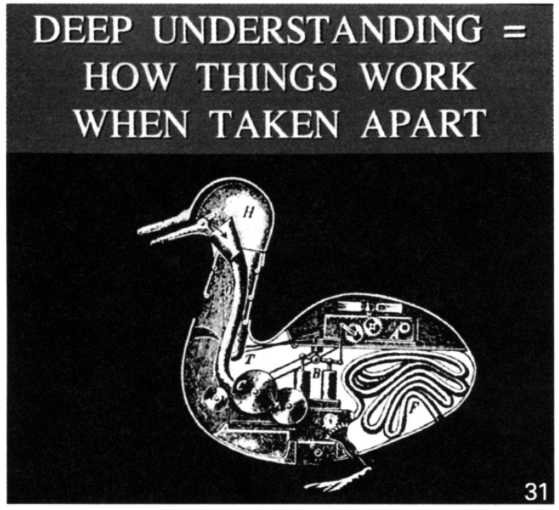
\includegraphics{./images/duck.png}

}

\caption{duck yeah}

\end{figure}%

What does it mean for \textbf{this} to cause \textbf{that}? This
question has flummoxed the discipline of statistics for a \emph{very}
long time; but, more than statistics, it has also flummoxed philosophers
for even longer!

Why is something that seems so natural to us in our limited, daily
lives, so difficult to formalize? If it is difficult for us to formalize
in conversation, how can we hope to formalize this so that a model can
\emph{discover} and \emph{evluate} causal effects from data?

Of all the weeks in this class, this is perhaps the most conceptually
challening.

\section{Learning Objectives}\label{learning-objectives-10}

At the end of this week's learning, students will be able to

\begin{enumerate}
\def\labelenumi{\arabic{enumi}.}
\tightlist
\item
  \textbf{Remember} that most interesting questions in their data
  analysis are actually causal questions.
\item
  \textbf{Articulate} a particular causal model that describes the
  world, and \textbf{evaluate} whether a research design and a
  statistical analysis does an adequate job answering a question about a
  causal model.
\item
  \textbf{Appreciate} the deep difficulty of causal questions, and how
  research design guides data collection.
\end{enumerate}

\section{Class Announcements}\label{class-announcements-9}

\textbf{Lab 2-Regression}

\textbf{Overview}

\begin{itemize}
\tightlist
\item
  \textbf{Setting}: You are data scientists for a maker of products.
\item
  \textbf{Task}: You select your own research question

  \begin{itemize}
  \tightlist
  \item
    Your X should be an aspect of product design
  \item
    Your Y should be a metric of product success
  \end{itemize}
\item
  \textbf{Deliverable}: A statistical analysis that includes

  \begin{itemize}
  \tightlist
  \item
    An introduction that motivates your research question
  \item
    A description of your model-building process
  \item
    A discussion of statistical assumptions that may be problematic
  \item
    A well-formatted regression table with a minimum of 3 specifications
  \item
    A conclusion that extracts key lessons from your statistical results
  \end{itemize}
\end{itemize}

\textbf{The Report}\\
- Writing for a collaborating data scientist, what research question
have you asked, what answers have you found, and how did you find them?

\begin{longtable}[]{@{}lll@{}}
\toprule\noalign{}
Deliverable Name & Week Due & Grade Weight \\
\midrule\noalign{}
\endhead
\bottomrule\noalign{}
\endlastfoot
Research Proposal & Week 12 & 10\% \\
Within-Team Review & Week 14 & 5\% \\
Final Presentation & Week 14 & 10\% \\
Final Report & Week 14 & 75\% \\
\end{longtable}

\textbf{Team Work Evaluation}

\begin{itemize}
\tightlist
\item
  Most data science work happens on teams.
\item
  Our educational goals include helping you improve in your role as a
  teammate.
\item
  We'll ask you to fill out a confidential evaluation regarding your
  team dynamics.
\end{itemize}

\textbf{Final Presentation}

\begin{itemize}
\tightlist
\item
  Team will present their work in live session 14.

  \begin{itemize}
  \tightlist
  \item
    Teams have between 10-15 min dedicated to discussing their work
    (depending on section size)
  \item
    Two-thirds of the time can be the team presenting
  \item
    \textbf{BUT} at least one-third should be asking and answering
    questions with your peers
  \item
    For example, if teams have 15 minutes total, then plan to present
    for no more than 10 minutes and structure 5 minutes of questions.
  \end{itemize}
\end{itemize}

\section{Roadmap}\label{roadmap-7}

\textbf{Rearview Mirror}

\begin{itemize}
\tightlist
\item
  Statisticians create a population model to represent the world.
\item
  The BLP is a useful way to summarize relationships in a model, and OLS
  regression is a way to estimate the BLP.
\item
  OLS regression is a foundational tool that can be applied to questions
  of description
\end{itemize}

\textbf{Today}

\begin{itemize}
\tightlist
\item
  Questions of explanation require a substantially different modeling
  process.
\item
  To answer causal questions, we must work within a causal theory
\item
  OLS regression is sometimes appropriate for measuring a causal effect,
\item
  But, only when the model estimated matches the causal theory.
\item
  So, we must watch out for omitted variable bias, reverse causality,
  and outcome variables on the right hand side.
\end{itemize}

\textbf{Looking Ahead}

\begin{itemize}
\tightlist
\item
  The famous Classical Linear Model (CLM) allows us to apply regression
  to smaller samples.
\item
  We will address the pervasive issue of false discovery, and ways to be
  a responsible member of the scientific community.
\end{itemize}

\section{Discussion}\label{discussion-1}

\subsection{Path Diagrams}\label{path-diagrams}

\[
\begin{matrix}
\\
\text{Sleep} \rightarrow \text{Feelings of Stress} \\
\\
\end{matrix}
\]

\begin{itemize}
\tightlist
\item
  How would the following fit into this causal path diagram?

  \begin{enumerate}
  \def\labelenumi{\arabic{enumi}.}
  \tightlist
  \item
    All the other factors in the world that also cause stress but don't
    have a causal relationship with sleep.
  \item
    A factor: Coffee Intake

    \begin{itemize}
    \tightlist
    \item
      What happens if you omit it in your regression?
    \end{itemize}
  \item
    Reverse causality
  \item
    An outcome variable on the RHS: Job Performance

    \begin{itemize}
    \tightlist
    \item
      What happens if you include it in your regression?
    \end{itemize}
  \end{enumerate}
\end{itemize}

\section{An Interlude}\label{an-interlude}

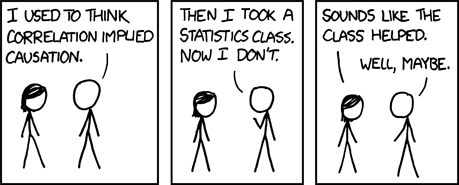
\includegraphics[width=0.8\textwidth,height=\textheight]{./images/correlation.png}

\subsection{Omitted Variable Bias}\label{omitted-variable-bias}

\begin{itemize}
\tightlist
\item
  Recall the equation for omitted variable bias
\end{itemize}

\includegraphics[width=0.8\textwidth,height=\textheight]{images/ovb.png}

\begin{itemize}
\tightlist
\item
  What specific regressions do \(\beta_2\) and \(\gamma_1\) come from?
\end{itemize}

\section{R Exercise}\label{r-exercise-2}

\subsection{Omitted Variable Bias in
R}\label{omitted-variable-bias-in-r}

The file \texttt{htv.RData} contains data from the 1991 National
Longitudinal Survey of Youth, provided by Wooldridge. All people in the
sample are males age 26 to 34. The data is interesting here, because it
includes education, stored in the variable \texttt{educ}, and also a
score on an ability test, stored in the variable \texttt{abil}.

\begin{Shaded}
\begin{Highlighting}[]
\FunctionTok{load}\NormalTok{(}\StringTok{\textquotesingle{}./data/htv.RData\textquotesingle{}}\NormalTok{)}

\NormalTok{data }\OtherTok{\textless{}{-}}\NormalTok{ data }\SpecialCharTok{|\textgreater{}}  
  \FunctionTok{rename}\NormalTok{(}
    \AttributeTok{ability    =}\NormalTok{ abil, }
    \AttributeTok{education  =}\NormalTok{ educ, }
    \AttributeTok{north\_east =}\NormalTok{ ne, }
    \AttributeTok{north\_cent =}\NormalTok{ nc, }
    \AttributeTok{potential\_experience =}\NormalTok{ exper, }
    \AttributeTok{edu\_mother =}\NormalTok{ motheduc, }
    \AttributeTok{edu\_father =}\NormalTok{ fatheduc, }
    \AttributeTok{divorce\_14 =}\NormalTok{ brkhme14, }
    \AttributeTok{siblings   =}\NormalTok{ sibs, }
    \AttributeTok{tuition\_17 =}\NormalTok{ tuit17, }
    \AttributeTok{tuition\_18 =}\NormalTok{ tuit18) }\SpecialCharTok{|\textgreater{}}  
  \FunctionTok{mutate}\NormalTok{(}
    \AttributeTok{education\_f =} \FunctionTok{cut}\NormalTok{(education, }\AttributeTok{breaks =} \FunctionTok{c}\NormalTok{(}\DecValTok{0}\NormalTok{,}\DecValTok{12}\NormalTok{,}\DecValTok{16}\NormalTok{,}\DecValTok{100}\NormalTok{))) }\SpecialCharTok{|\textgreater{}} 
  \FunctionTok{select}\NormalTok{(}\SpecialCharTok{{-}}\FunctionTok{c}\NormalTok{(ctuit, expersq, lwage))}
  
\FunctionTok{glimpse}\NormalTok{(data)}
\end{Highlighting}
\end{Shaded}

\begin{verbatim}
Rows: 1,230
Columns: 21
$ wage                 <dbl> 12.019231, 8.912656, 15.514334, 13.333333, 11.070~
$ ability              <dbl> 5.0277381, 2.0371704, 2.4758952, 3.6092398, 2.636~
$ education            <int> 15, 13, 15, 15, 13, 18, 13, 12, 13, 12, 12, 12, 1~
$ north_east           <int> 0, 1, 1, 1, 1, 1, 1, 0, 1, 1, 1, 1, 0, 1, 1, 1, 1~
$ north_cent           <int> 0, 0, 0, 0, 0, 0, 0, 0, 0, 0, 0, 0, 0, 0, 0, 0, 0~
$ west                 <int> 1, 0, 0, 0, 0, 0, 0, 0, 0, 0, 0, 0, 1, 0, 0, 0, 0~
$ south                <int> 0, 0, 0, 0, 0, 0, 0, 1, 0, 0, 0, 0, 0, 0, 0, 0, 0~
$ potential_experience <int> 9, 8, 11, 6, 15, 8, 13, 14, 9, 9, 13, 14, 4, 8, 7~
$ edu_mother           <int> 12, 12, 12, 12, 12, 12, 13, 12, 10, 14, 9, 12, 17~
$ edu_father           <int> 12, 10, 16, 12, 15, 12, 12, 12, 12, 12, 10, 16, 1~
$ divorce_14           <int> 0, 1, 0, 0, 1, 0, 0, 1, 1, 0, 1, 0, 0, 0, 0, 0, 0~
$ siblings             <int> 1, 4, 2, 1, 2, 2, 5, 4, 3, 1, 2, 1, 1, 3, 2, 2, 1~
$ urban                <int> 1, 1, 1, 1, 1, 1, 1, 0, 1, 1, 1, 0, 1, 1, 1, 1, 1~
$ ne18                 <int> 1, 1, 1, 1, 1, 1, 1, 1, 1, 1, 1, 1, 1, 1, 1, 1, 1~
$ nc18                 <int> 0, 0, 0, 0, 0, 0, 0, 0, 0, 0, 0, 0, 0, 0, 0, 0, 0~
$ south18              <int> 0, 0, 0, 0, 0, 0, 0, 0, 0, 0, 0, 0, 0, 0, 0, 0, 0~
$ west18               <int> 0, 0, 0, 0, 0, 0, 0, 0, 0, 0, 0, 0, 0, 0, 0, 0, 0~
$ urban18              <int> 1, 1, 1, 1, 1, 1, 1, 1, 1, 1, 1, 1, 1, 1, 1, 1, 1~
$ tuition_17           <dbl> 7.582914, 8.595144, 7.311346, 9.499537, 7.311346,~
$ tuition_18           <dbl> 7.260242, 9.499537, 7.311346, 10.162070, 7.311346~
$ education_f          <fct> "(12,16]", "(12,16]", "(12,16]", "(12,16]", "(12,~
\end{verbatim}

\begin{Shaded}
\begin{Highlighting}[]
\NormalTok{wage\_plot }\OtherTok{\textless{}{-}}\NormalTok{ data }\SpecialCharTok{|\textgreater{}}  
  \FunctionTok{ggplot}\NormalTok{() }\SpecialCharTok{+} 
  \FunctionTok{aes}\NormalTok{(}\AttributeTok{x=}\NormalTok{wage, }\AttributeTok{fill=}\NormalTok{education\_f) }\SpecialCharTok{+} 
  \FunctionTok{geom\_histogram}\NormalTok{(}\AttributeTok{bins=}\DecValTok{30}\NormalTok{)}
\NormalTok{ability\_plot }\OtherTok{\textless{}{-}}\NormalTok{ data }\SpecialCharTok{|\textgreater{}}  
  \FunctionTok{ggplot}\NormalTok{() }\SpecialCharTok{+} 
  \FunctionTok{aes}\NormalTok{(}\AttributeTok{x=}\NormalTok{ability, }\AttributeTok{fill=}\NormalTok{education\_f) }\SpecialCharTok{+} 
  \FunctionTok{geom\_histogram}\NormalTok{(}\AttributeTok{bins=}\DecValTok{30}\NormalTok{)}
\NormalTok{wage\_by\_ability\_plot }\OtherTok{\textless{}{-}}\NormalTok{ data }\SpecialCharTok{|\textgreater{}}  
  \FunctionTok{ggplot}\NormalTok{() }\SpecialCharTok{+} 
  \FunctionTok{aes}\NormalTok{(}\AttributeTok{x=}\NormalTok{ability, }\AttributeTok{y=}\NormalTok{wage, }\AttributeTok{color=}\NormalTok{education\_f) }\SpecialCharTok{+} 
  \FunctionTok{geom\_point}\NormalTok{()}
  

\NormalTok{(wage\_plot }\SpecialCharTok{|}\NormalTok{ ability\_plot) }\SpecialCharTok{/} 
\NormalTok{  wage\_by\_ability\_plot}
\end{Highlighting}
\end{Shaded}

\includegraphics{11-causal-models_files/figure-pdf/unnamed-chunk-2-1.pdf}

Assume that the true model is,

\includegraphics[width=0.8\textwidth,height=\textheight]{images/wage_system.png}

\subsection{Questions:}\label{questions}

\begin{enumerate}
\def\labelenumi{\arabic{enumi}.}
\tightlist
\item
  Are we able to \emph{directly} measure ability? If so, how would you
  propose to measure it?
\item
  If not, what \emph{do} we measure and how is this measurement related
  to ability? And there is a lot of evidence to suggest that
  standardized tests are not a very good proxy. But for now, let's
  pretend that we really are measuring ability.
\item
  Using R, estimate (a) the true model, and (b) the regression of
  ability on education.
\item
  Write down the expression for what omitted variable bias would be if
  you couldn't measure ability.\\
\item
  Add this omitted variable bias to the coefficient for education to see
  what it would be.
\item
  Now evaluate your previous result by fitting the model,
  \[wage = \alpha_0 + \alpha_1 educ + w\]
\item
  Does the coefficient for the relationship between education and wages
  match what you estimated earlier?
\item
  Why or why not?
\item
  Reflect on your results:
\item
  What does the direction of omitted variable bias suggest about OLS
  estimates of returns to education?\\
\item
  What does this suggest about the reported statistical significance of
  education?
\end{enumerate}

\section{Research Design Strategies}\label{research-design-strategies}

Hopefully you feel like, ``Golly. It would be really, \emph{really} hard
to assert some causal model and \emph{know that it is actually true}.''
How does this lead you to think about the role of research design in
setting up your data collection?

\begin{enumerate}
\def\labelenumi{\arabic{enumi}.}
\tightlist
\item
  If you could \textbf{do the experiment} to determine the effect of
  education on wages, how would you do it?
\item
  If you cannot \textbf{do the experiment} to determine the effect of
  education on wages, what are some options for where to look for data?
  What would you hope these areas provide to you?
\end{enumerate}

\section{Discussion}\label{discussion-2}

\textbf{The Direction of Omitted Variable Bias}

\begin{itemize}
\tightlist
\item
  For each regression, estimate whether omitted variable bias is towards
  zero or away from zero.
\end{itemize}

\begin{longtable}[]{@{}
  >{\raggedright\arraybackslash}p{(\columnwidth - 2\tabcolsep) * \real{0.5976}}
  >{\raggedright\arraybackslash}p{(\columnwidth - 2\tabcolsep) * \real{0.4024}}@{}}
\toprule\noalign{}
\begin{minipage}[b]{\linewidth}\raggedright
Regression Output
\end{minipage} & \begin{minipage}[b]{\linewidth}\raggedright
Omitted Variable
\end{minipage} \\
\midrule\noalign{}
\endhead
\bottomrule\noalign{}
\endlastfoot
\(\widehat{grade} = 72.1 + 0.4\ attendance\) & \(time\_studying\) \\
\(\widehat{lifespan} = 87.4 - 1.2\ cigarettes\) & \(exercise\) \\
\(\widehat{lifespan} = 87.4 - 1.2\ cigarettes\) &
\(time\_socializing\) \\
\(\widehat{wage} = 14.0 + 2.1\ grad\_education\) & \(experience\) \\
\(\widehat{wage} = 14.0 + 2.1\ grad\_education\) & desire to effect
\(social\_good\) \\
\(\widehat{literacy} = 54 + 12\ network\_access\) & \(wealth\) \\
\end{longtable}

\chapter{The Classical Linear Model}\label{the-classical-linear-model}

\section{Learning Objectives}\label{learning-objectives-11}

At the end of this week's learning students will be able to

\begin{enumerate}
\def\labelenumi{\arabic{enumi}.}
\tightlist
\item
  \textbf{Describe} the assumptions of the classical linear model
  (sometimes referred to as the Gauss-Markov Assumptions) and what each
  assumption contributes to the estimator.
\item
  \textbf{Evaluate} using empirical methods, whether each of the
  assumptions are likely to be true of the population data generating
  function.
\item
  \textbf{Assess} whether the guarantees that are provided by the
  classical linear model's requirements are likely to \emph{ever} be
  true, including within data the student is likely to encounter.
\end{enumerate}

\section{Class Announcements}\label{class-announcements-10}

\begin{itemize}
\tightlist
\item
  Lab 2 Deliverable and Dates

  \begin{itemize}
  \tightlist
  \item
    Research Proposal (Today)
  \item
    Within-Team Review (Week 14)
  \item
    Final Report (Week 14)
  \item
    Final Presentation (Week 14)
  \end{itemize}
\end{itemize}

\section{Roadmap}\label{roadmap-8}

\textbf{Rearview Mirror}

\begin{itemize}
\tightlist
\item
  Statisticians create a population model to represent the world.
\item
  The BLP is a useful summary for a relationship among random variables.
\item
  OLS regression is an estimator for the Best Linear Predictor (BLP).
\item
  For a large sample, we only need two mild assumptions to work with OLS

  \begin{itemize}
  \tightlist
  \item
    To know coefficients are consistent
  \item
    To have valid standard errors, hypothesis tests
  \end{itemize}
\end{itemize}

\textbf{Today}

\begin{itemize}
\tightlist
\item
  The Classical Linear Model (CLM) allows us to apply regression to
  smaller samples.
\item
  The CLM requires more to be true of the data generating process, to
  make coefficients, standard errors, and tests \emph{meaningful} in
  small samples.
\item
  Understanding if the data meets these requirements (often called
  assumptions) requires considerable care.
\end{itemize}

\textbf{Looking Ahead}

\begin{itemize}
\tightlist
\item
  The CLM -- and the methods that we use to evaluate the CLM -- are the
  basis of advanced models (\emph{inter alia} time-series)
\item
  (Week 13) In a regression studies (and other studies), false discovery
  is a widespread problem. Understanding its causes can make you a
  better member of the scientific community.
\end{itemize}

\section{The Classical Linear Model}\label{the-classical-linear-model-1}

Comparing the Large Sample Model and the CLM

\subsection{Part 1}\label{part-1-1}

\begin{itemize}
\tightlist
\item
  We say that in small samples, more needs be true of our data for OLS
  regression to ``work.''

  \begin{itemize}
  \tightlist
  \item
    What do we mean when we say ``work''?

    \begin{itemize}
    \tightlist
    \item
      If our goals are descriptive, how is a ``working'' estimator
      useful?
    \item
      If our goals are explanatory, how is a ``working'' estimator
      useful?
    \item
      If our goals are predictive, are the requirements the same?
    \end{itemize}
  \end{itemize}
\end{itemize}

\subsection{Part 2}\label{part-2-1}

\begin{itemize}
\tightlist
\item
  Suppose that you're interested in understanding how subsidized school
  meals benefit under-resourced students in San Francisco East Bay
  region.

  \begin{itemize}
  \tightlist
  \item
    Using the tools from DATASCI 201, refine this question to a data
    science question.
  \item
    Suppose that there exists two possible data sources to answer the
    question you have formed:

    \begin{itemize}
    \tightlist
    \item
      A large amount (e.g.~10,000 data points) of individual-level data
      about income, nutrition and test scores, self-reported by
      individual families who have opted in to the study.\\
    \item
      A relatively smaller amount (e.g.~500 data points) of Government
      data about school district characteristics, including
      district-level college achievement; county-level home prices, and
      state-level tax receipts.
    \end{itemize}
  \end{itemize}
\item
  \textbf{What are the tradeoffs to using one or the other data
  source?}\\
\end{itemize}

\subsection{Part 3}\label{part-3-1}

\begin{itemize}
\tightlist
\item
  Suppose you elect to use the relatively larger sample of
  individual-level data.

  \begin{itemize}
  \tightlist
  \item
    Which of the large-sample assumptions do you expect are valid, and
    which are problematic?
  \end{itemize}
\item
  Or, suppose that you elect to use the relatively smaller sample of
  school-district-level data.

  \begin{itemize}
  \tightlist
  \item
    Which of the CLM assumptions do you expect are valid, and which do
    you expect are most problematic?
  \end{itemize}
\item
  \textbf{What was the research question that you identified?}
\item
  \textbf{What would a successful answer accomplish?}
\end{itemize}

\subsection{Part 4}\label{part-4}

\begin{itemize}
\tightlist
\item
  \textbf{Which data source, the individual or the district-level, do
  you think is more likely to produce a successful answer?}
\end{itemize}

\subsection{Part 5}\label{part-5}

Problems with the CLM Requirements

\begin{itemize}
\item
  There are five requirements for the CLM

  \begin{enumerate}
  \def\labelenumi{\arabic{enumi}.}
  \tightlist
  \item
    IID Sampling
  \item
    Linear Conditional Expectation
  \item
    No Perfect Collinearity
  \item
    Homoskedastic Errors
  \item
    Normally Distributed Errors
  \end{enumerate}
\item
  For each of these requirements:

  \begin{itemize}
  \tightlist
  \item
    Identify one \textbf{concrete} way that the data might not satisfy
    the requirement.
  \item
    Identify what the consequence of failing to satisfy the requirement
    would be.
  \item
    Identify a path forward to satisfy the requirement.
  \end{itemize}
\end{itemize}

\section{R Exercise}\label{r-exercise-3}

\begin{Shaded}
\begin{Highlighting}[]
\FunctionTok{library}\NormalTok{(tidyverse)}
\FunctionTok{library}\NormalTok{(wooldridge)}
\FunctionTok{library}\NormalTok{(car)}
\FunctionTok{library}\NormalTok{(lmtest)}
\FunctionTok{library}\NormalTok{(sandwich)}
\FunctionTok{library}\NormalTok{(stargazer)}
\end{Highlighting}
\end{Shaded}

If you haven't used the \texttt{mtcars} dataset, you haven't been
through an intro applied stats class!

In this analysis, we will use the mtcars dataset which is a dataset that
was extracted from the 1974 Motor Trend US magazine, and comprises fuel
consumption and 10 aspects of automobile design and performance for 32
automobiles (1973-74 models). The dataset is automatically available
when you start R.

For more information about the dataset, use the R command:
\texttt{help(mtcars)}

\begin{Shaded}
\begin{Highlighting}[]
\FunctionTok{data}\NormalTok{(mtcars)}
\FunctionTok{glimpse}\NormalTok{(mtcars)}
\end{Highlighting}
\end{Shaded}

\begin{verbatim}
Rows: 32
Columns: 11
$ mpg  <dbl> 21.0, 21.0, 22.8, 21.4, 18.7, 18.1, 14.3, 24.4, 22.8, 19.2, 17.8,~
$ cyl  <dbl> 6, 6, 4, 6, 8, 6, 8, 4, 4, 6, 6, 8, 8, 8, 8, 8, 8, 4, 4, 4, 4, 8,~
$ disp <dbl> 160.0, 160.0, 108.0, 258.0, 360.0, 225.0, 360.0, 146.7, 140.8, 16~
$ hp   <dbl> 110, 110, 93, 110, 175, 105, 245, 62, 95, 123, 123, 180, 180, 180~
$ drat <dbl> 3.90, 3.90, 3.85, 3.08, 3.15, 2.76, 3.21, 3.69, 3.92, 3.92, 3.92,~
$ wt   <dbl> 2.620, 2.875, 2.320, 3.215, 3.440, 3.460, 3.570, 3.190, 3.150, 3.~
$ qsec <dbl> 16.46, 17.02, 18.61, 19.44, 17.02, 20.22, 15.84, 20.00, 22.90, 18~
$ vs   <dbl> 0, 0, 1, 1, 0, 1, 0, 1, 1, 1, 1, 0, 0, 0, 0, 0, 0, 1, 1, 1, 1, 0,~
$ am   <dbl> 1, 1, 1, 0, 0, 0, 0, 0, 0, 0, 0, 0, 0, 0, 0, 0, 0, 1, 1, 1, 0, 0,~
$ gear <dbl> 4, 4, 4, 3, 3, 3, 3, 4, 4, 4, 4, 3, 3, 3, 3, 3, 3, 4, 4, 4, 3, 3,~
$ carb <dbl> 4, 4, 1, 1, 2, 1, 4, 2, 2, 4, 4, 3, 3, 3, 4, 4, 4, 1, 2, 1, 1, 2,~
\end{verbatim}

\subsection{Questions:}\label{questions-1}

\begin{enumerate}
\def\labelenumi{\arabic{enumi}.}
\setcounter{enumi}{-1}
\tightlist
\item
  Using the \texttt{mtcars} data, quickly reason about the variables
  that we're interested in studying:
\end{enumerate}

\begin{Shaded}
\begin{Highlighting}[]
\NormalTok{mtcars }\SpecialCharTok{\%\textgreater{}\%} 
  \FunctionTok{ggplot}\NormalTok{() }\SpecialCharTok{+} 
  \FunctionTok{aes}\NormalTok{(}\AttributeTok{x=}\NormalTok{mpg) }\SpecialCharTok{+}
  \FunctionTok{geom\_histogram}\NormalTok{(}\AttributeTok{bins=}\DecValTok{10}\NormalTok{)}
\end{Highlighting}
\end{Shaded}

\includegraphics{12-classical-linear-model_files/figure-pdf/unnamed-chunk-3-1.pdf}

\begin{Shaded}
\begin{Highlighting}[]
\NormalTok{mtcars }\SpecialCharTok{\%\textgreater{}\%} 
  \FunctionTok{select}\NormalTok{(mpg, disp, hp, wt, drat) }\SpecialCharTok{\%\textgreater{}\%} 
  \FunctionTok{pairs}\NormalTok{(}\AttributeTok{pch=}\DecValTok{19}\NormalTok{)}
\end{Highlighting}
\end{Shaded}

\includegraphics{12-classical-linear-model_files/figure-pdf/unnamed-chunk-3-2.pdf}

\begin{enumerate}
\def\labelenumi{\arabic{enumi}.}
\tightlist
\item
  Using the \texttt{mtcars} data, run a linear regression to find the
  relationship between miles per gallon (\texttt{mpg}) on the
  left-hand-side as a function of displacement (\texttt{disp}), gross
  horsepower (\texttt{hp}), weight (\texttt{wt}), and rear axle ratio
  (\texttt{drat}) on the right-hand-side. That is, fit a regression of
  the following form:
\end{enumerate}

\[
\widehat{mpg} = \hat{\beta_{0}} + \hat{\beta}_{1} disp + \hat{\beta}_{2}horse\_power + \hat{\beta}_{3}weight + \hat{\beta}_{4}drive\_ratio
\]

\begin{enumerate}
\def\labelenumi{\arabic{enumi}.}
\setcounter{enumi}{1}
\tightlist
\item
  For \textbf{each} of the following CLM assumptions, assess whether the
  assumption holds. Where possible, demonstrate multiple ways of
  assessing an assumption. When an assumption appears violated, state
  what steps you would take in response.

  \begin{itemize}
  \tightlist
  \item
    I.I.D. data
  \item
    Linear conditional expectation
  \item
    No perfect collinearity
  \item
    Homoskedastic errors
  \item
    Normally distributed errors
  \end{itemize}
\end{enumerate}

\begin{Shaded}
\begin{Highlighting}[]
\CommentTok{\# goal:}
\CommentTok{\# consequence if violated:}
\end{Highlighting}
\end{Shaded}

\begin{Shaded}
\begin{Highlighting}[]
\CommentTok{\# goal:}
\CommentTok{\# consequence if violated:}
\end{Highlighting}
\end{Shaded}

\begin{Shaded}
\begin{Highlighting}[]
\CommentTok{\# goal:}
\CommentTok{\# consequence if violated:}
\end{Highlighting}
\end{Shaded}

\begin{Shaded}
\begin{Highlighting}[]
\CommentTok{\# goal:}
\CommentTok{\# consequence if violated:}
\end{Highlighting}
\end{Shaded}

\begin{Shaded}
\begin{Highlighting}[]
\CommentTok{\# goal:}
\CommentTok{\# consequence if violated:}
\end{Highlighting}
\end{Shaded}

\begin{enumerate}
\def\labelenumi{\arabic{enumi}.}
\setcounter{enumi}{2}
\item
  In addition to the above, assess to what extent (imperfect)
  collinearity is affecting your inference.
\item
  Interpret the coefficient on horsepower.
\item
  Perform a hypothesis test to assess whether rear axle ratio has an
  effect on mpg. What assumptions need to be true for this hypothesis
  test to be informative? Are they?
\item
  Choose variable transformations (if any) for each variable, and try to
  better meet the assumptions of the CLM (which also maintaining the
  readability of your model).
\item
  (As time allows) report the results of both models in a nicely
  formatted regression table.
\end{enumerate}

\chapter{Reproducible Research}\label{reproducible-research}

\section{Learning Objectives}\label{learning-objectives-12}

\begin{enumerate}
\def\labelenumi{\arabic{enumi}.}
\tightlist
\item
\item
\item
\end{enumerate}

\section{Class Announcements}\label{class-announcements-11}

\section{Roadmap}\label{roadmap-9}

\textbf{Rearview Mirror}

\textbf{Today}

\textbf{Looking Ahead}

\section{What data science hopes to
accomplish}\label{what-data-science-hopes-to-accomplish}

\begin{itemize}
\tightlist
\item
  As a data scientist, our goal is to learn about the world:

  \begin{itemize}
  \tightlist
  \item
    \emph{Theorists} and \emph{theologians} build systems of
    explanations that are consistent with themselves
  \item
    \emph{Analysts} build systems of explanations that are consistent
    with the past
  \item
    \emph{Scientists} build systems of explanations that usefully
    predict events, \textbf{or data}, that hasn't yet been seen
  \end{itemize}
\end{itemize}

\section{Learning from Data}\label{learning-from-data}

\begin{itemize}
\tightlist
\item
  As a data scientist, the way we learn about the world is through the
  streams of data that \textbf{real world} events produce

  \begin{itemize}
  \tightlist
  \item
    Machine processes
  \item
    Political outcomes
  \item
    Customer actions
  \end{itemize}
\item
  The watershed moment in our field has been the profusion of data
  available, from many places, that is richer than at any other point in
  our past.

  \begin{itemize}
  \tightlist
  \item
    In 251, and 266 we place structure on data series like audio, video
    and text that are \emph{transcendently} rich
  \item
    In 261 we bring together flows of data that are generated at massive
    scales
  \item
    In 209 we ask, ``How can we take data, and produce a \emph{new} form
    of it that is most effectively understood by the human visual and
    interactive mind?
  \end{itemize}
\end{itemize}

\section{Data Science and Statistics}\label{data-science-and-statistics}

\begin{itemize}
\tightlist
\item
  So why statistics?
\item
  And why the way we've chosen to approach statistics in 203?
\end{itemize}

\section{Why Statistics?: A Closing Argument for
Statistics}\label{why-statistics-a-closing-argument-for-statistics}

\begin{itemize}
\item
  Business, policy, education and medical decisions are made \emph{by
  humans} based on data
\item
  A central task when we observe some pattern in data is to
  \textbf{infer} whether the pattern will occur in some novel context
\item
  Statistics, as we practice it in 203, allows us to characterize:

  \begin{itemize}
  \tightlist
  \item
    What we have seen
  \item
    What we \emph{could have seen}
  \item
    Whether any guarantees exist about what we have seen
  \item
    What we can infer about the population
  \end{itemize}
\item
  So that we can either describe, explain or predict behavior.
\end{itemize}

\section{Course Goals}\label{course-goals}

\subsection{Course Section III: Purpose-Driven
Models}\label{course-section-iii-purpose-driven-models}

\begin{itemize}
\item
  Statistical models are unknowing transformations of data

  \begin{itemize}
  \tightlist
  \item
    Because they're built on the foundation of probability, we have
    certain guarantees what a model ``says''
  \item
    Because they're unknowing, the models themselves know-not what they
    say.
  \end{itemize}
\item
  As the data scientist, bring them alive to achieve our modeling goals
\item
  In Lab 2 we have expanded our ability to parse the world using
  regression, built a model that accomplishes our goals, and done so in
  a way that brings the ability to test under a \emph{``null''} scenario

  \begin{itemize}
  \tightlist
  \item
    \textbf{Key insight}: regression is little more than conditional
    averages
  \end{itemize}
\end{itemize}

\subsection{Course Section II: Sampling Theory and
Testing}\label{course-section-ii-sampling-theory-and-testing}

\begin{itemize}
\tightlist
\item
  Under \textbf{very} general assumptions, sample averages follow a
  predictable, known, distribution -- the \emph{Gaussian distribution}
\item
  This is true, even when the underlying probability distribution is
  \emph{very} complex, or unknown!
\item
  Due to this common distribution, we can produce reliable, general
  tests!
\item
  In Lab 1 we computed simple statistics, and used guarantees from
  sampling theory to \textbf{test} whether these differences were likely
  to arise under a \emph{``null''} scenario
\end{itemize}

\subsection{Course Section I: Probability
Theory}\label{course-section-i-probability-theory}

\begin{itemize}
\tightlist
\item
  Probability theory

  \begin{itemize}
  \tightlist
  \item
    Underlies modeling and regression (Part III);
  \item
    Underlies sampling, inference, and testing (Part II)
  \item
    \textbf{Every} model built in \textbf{every} corner of data science
  \end{itemize}
\end{itemize}

We can:

\begin{itemize}
\tightlist
\item
  Model the complex world that we live in using probability theory;
\item
  Move from a probability density function that is defined in terms of a
  single variable, into a function that is defined in terms of many
  variables
\item
  Compute useful summaries -- i.e.~the BLP, expected value, and
  covariance -- even with \emph{highly} complex probability density
  functions.
\end{itemize}

\subsection{Statistics as a Foundation for
MIDS}\label{statistics-as-a-foundation-for-mids}

\begin{itemize}
\tightlist
\item
  In w203, we hope to have laid a foundation in probability that can be
  used not only in statistical applications, but also in every other
  machine learning application that are likely to ever encounter
\end{itemize}

\section{Reproducibility Discussion}\label{reproducibility-discussion}

\textbf{Green Jelly Beans}

\textbf{What went wrong here?}

\subsection{Discussion}\label{discussion-3}

\textbf{Status Update} You have a dataset of the number of Facebook
status updates by day of the week. You run 7 different t-tests, one for
posts on Monday (versus all other days), or for Tuesday (versus all
other days), etc. Only the test for Sunday is significant, with a
p-value of .045, so you throw out the other tests.

Should you conclude that Sunday has a significant effect on number of
posts? (How can you address this situation responsibly when you publish
your results?)

\textbf{Such Update} As before, you have a dataset of the number of
Facebook status updates by day of the week. You do a little EDA and
notice that Sunday seems to have more ``status updates'' than all other
days, so you recode your ``day of the week'' variable into a binary one:
Sunday = 1, All other days = 0. You run a t-test and get a p-value of
.045. Should you conclude that Sunday has a significant effect on number
of posts?

\textbf{Sunday Funday} Suppose researcher A tests if Monday has an
effect (versus all other days), Researcher B tests Tuesday (versus all
other days), and so forth. Only Researcher G, who tests Sunday finds a
significant effect with a p-value of .045. Only Researcher G gets to
publish her work. If you read the paper, should you conclude that Sunday
has a significant effect on number of posts?

\textbf{Sunday Repentence} What if researcher G above is a sociologist
that chooses to measure the effect of Sunday based on years of observing
the way people behave on weekends? Researcher G is not interested in the
other tests, because Sunday is the interesting day from her perspective,
and she wouldn't expect any of the other tests to be significant.

\textbf{Decreasing Effect Sizes} Many observers have noted that as
studies yielding statistically significant results are repeated,
estimated effect sizes go down and often become insignificant. Why is
this the case?



\end{document}
